% Options for packages loaded elsewhere
\PassOptionsToPackage{unicode}{hyperref}
\PassOptionsToPackage{hyphens}{url}
%
\documentclass[
]{article}
\usepackage{lmodern}
\usepackage{amssymb,amsmath}
\usepackage{ifxetex,ifluatex}
\ifnum 0\ifxetex 1\fi\ifluatex 1\fi=0 % if pdftex
  \usepackage[T1]{fontenc}
  \usepackage[utf8]{inputenc}
  \usepackage{textcomp} % provide euro and other symbols
\else % if luatex or xetex
  \usepackage{unicode-math}
  \defaultfontfeatures{Scale=MatchLowercase}
  \defaultfontfeatures[\rmfamily]{Ligatures=TeX,Scale=1}
\fi
% Use upquote if available, for straight quotes in verbatim environments
\IfFileExists{upquote.sty}{\usepackage{upquote}}{}
\IfFileExists{microtype.sty}{% use microtype if available
  \usepackage[]{microtype}
  \UseMicrotypeSet[protrusion]{basicmath} % disable protrusion for tt fonts
}{}
\makeatletter
\@ifundefined{KOMAClassName}{% if non-KOMA class
  \IfFileExists{parskip.sty}{%
    \usepackage{parskip}
  }{% else
    \setlength{\parindent}{0pt}
    \setlength{\parskip}{6pt plus 2pt minus 1pt}}
}{% if KOMA class
  \KOMAoptions{parskip=half}}
\makeatother
\usepackage{xcolor}
\IfFileExists{xurl.sty}{\usepackage{xurl}}{} % add URL line breaks if available
\IfFileExists{bookmark.sty}{\usepackage{bookmark}}{\usepackage{hyperref}}
\hypersetup{
  pdftitle={Práctica Machine Learning},
  pdfauthor={Fernández Hernández, Alberto},
  hidelinks,
  pdfcreator={LaTeX via pandoc}}
\urlstyle{same} % disable monospaced font for URLs
\usepackage[margin=1in]{geometry}
\usepackage{color}
\usepackage{fancyvrb}
\newcommand{\VerbBar}{|}
\newcommand{\VERB}{\Verb[commandchars=\\\{\}]}
\DefineVerbatimEnvironment{Highlighting}{Verbatim}{commandchars=\\\{\}}
% Add ',fontsize=\small' for more characters per line
\usepackage{framed}
\definecolor{shadecolor}{RGB}{248,248,248}
\newenvironment{Shaded}{\begin{snugshade}}{\end{snugshade}}
\newcommand{\AlertTok}[1]{\textcolor[rgb]{0.94,0.16,0.16}{#1}}
\newcommand{\AnnotationTok}[1]{\textcolor[rgb]{0.56,0.35,0.01}{\textbf{\textit{#1}}}}
\newcommand{\AttributeTok}[1]{\textcolor[rgb]{0.77,0.63,0.00}{#1}}
\newcommand{\BaseNTok}[1]{\textcolor[rgb]{0.00,0.00,0.81}{#1}}
\newcommand{\BuiltInTok}[1]{#1}
\newcommand{\CharTok}[1]{\textcolor[rgb]{0.31,0.60,0.02}{#1}}
\newcommand{\CommentTok}[1]{\textcolor[rgb]{0.56,0.35,0.01}{\textit{#1}}}
\newcommand{\CommentVarTok}[1]{\textcolor[rgb]{0.56,0.35,0.01}{\textbf{\textit{#1}}}}
\newcommand{\ConstantTok}[1]{\textcolor[rgb]{0.00,0.00,0.00}{#1}}
\newcommand{\ControlFlowTok}[1]{\textcolor[rgb]{0.13,0.29,0.53}{\textbf{#1}}}
\newcommand{\DataTypeTok}[1]{\textcolor[rgb]{0.13,0.29,0.53}{#1}}
\newcommand{\DecValTok}[1]{\textcolor[rgb]{0.00,0.00,0.81}{#1}}
\newcommand{\DocumentationTok}[1]{\textcolor[rgb]{0.56,0.35,0.01}{\textbf{\textit{#1}}}}
\newcommand{\ErrorTok}[1]{\textcolor[rgb]{0.64,0.00,0.00}{\textbf{#1}}}
\newcommand{\ExtensionTok}[1]{#1}
\newcommand{\FloatTok}[1]{\textcolor[rgb]{0.00,0.00,0.81}{#1}}
\newcommand{\FunctionTok}[1]{\textcolor[rgb]{0.00,0.00,0.00}{#1}}
\newcommand{\ImportTok}[1]{#1}
\newcommand{\InformationTok}[1]{\textcolor[rgb]{0.56,0.35,0.01}{\textbf{\textit{#1}}}}
\newcommand{\KeywordTok}[1]{\textcolor[rgb]{0.13,0.29,0.53}{\textbf{#1}}}
\newcommand{\NormalTok}[1]{#1}
\newcommand{\OperatorTok}[1]{\textcolor[rgb]{0.81,0.36,0.00}{\textbf{#1}}}
\newcommand{\OtherTok}[1]{\textcolor[rgb]{0.56,0.35,0.01}{#1}}
\newcommand{\PreprocessorTok}[1]{\textcolor[rgb]{0.56,0.35,0.01}{\textit{#1}}}
\newcommand{\RegionMarkerTok}[1]{#1}
\newcommand{\SpecialCharTok}[1]{\textcolor[rgb]{0.00,0.00,0.00}{#1}}
\newcommand{\SpecialStringTok}[1]{\textcolor[rgb]{0.31,0.60,0.02}{#1}}
\newcommand{\StringTok}[1]{\textcolor[rgb]{0.31,0.60,0.02}{#1}}
\newcommand{\VariableTok}[1]{\textcolor[rgb]{0.00,0.00,0.00}{#1}}
\newcommand{\VerbatimStringTok}[1]{\textcolor[rgb]{0.31,0.60,0.02}{#1}}
\newcommand{\WarningTok}[1]{\textcolor[rgb]{0.56,0.35,0.01}{\textbf{\textit{#1}}}}
\usepackage{graphicx}
\makeatletter
\def\maxwidth{\ifdim\Gin@nat@width>\linewidth\linewidth\else\Gin@nat@width\fi}
\def\maxheight{\ifdim\Gin@nat@height>\textheight\textheight\else\Gin@nat@height\fi}
\makeatother
% Scale images if necessary, so that they will not overflow the page
% margins by default, and it is still possible to overwrite the defaults
% using explicit options in \includegraphics[width, height, ...]{}
\setkeys{Gin}{width=\maxwidth,height=\maxheight,keepaspectratio}
% Set default figure placement to htbp
\makeatletter
\def\fps@figure{htbp}
\makeatother
\setlength{\emergencystretch}{3em} % prevent overfull lines
\providecommand{\tightlist}{%
  \setlength{\itemsep}{0pt}\setlength{\parskip}{0pt}}
\setcounter{secnumdepth}{-\maxdimen} % remove section numbering
\usepackage[font={small}]{caption}
\usepackage[document]{ragged2e}

\title{Práctica Machine Learning}
\author{Fernández Hernández, Alberto}
\date{4/28/2021}

\begin{document}
\maketitle

\justify

\begin{verbatim}
                                         [IIIII]
                                          )"""(
                                         /     \
                                        /       \
                                        |`-...-'|
                                        |aspirin|
                                      _ |`-...-'|    _
                                     (\)`-.___.(I) _(/)
                                       (I)  (/)(I)(\)
                                          (I)        
\end{verbatim}

\textbf{Nota}: a lo largo de la práctica, tanto en el tuneo de
hiperparámetros como en la comparación de modelos se ha llevado a cabo
mediante \textbf{validación cruzada repetida}, con la misma semilla
(1234) y nº de grupos (5).

\newpage

\hypertarget{introducciuxf3n-y-descripciuxf3n-de-los-datos}{%
\section{1. Introducción y descripción de los
datos}\label{introducciuxf3n-y-descripciuxf3n-de-los-datos}}

El objetivo del presente proyecto consiste en \textbf{elaborar un modelo
de clasificación binaria que permita predecir si un paciente presentará
o será más propenso a padecer una complicación hospitalaria tras una
intervención quirúrgica \footnote{\url{https://www.kaggle.com/omnamahshivai/surgical-dataset-binary-classification}}}.
Originalmente, el fichero (extraído de la plataforma Kaggle) contiene
tres variables objetivo, dos continuas:

\begin{enumerate}
\def\labelenumi{\arabic{enumi}.}
\tightlist
\item
  \emph{ccsComplicationRate}: incidencia general de complicaciones
  hospitalarias por cada tipo de intervención quirúrgica.
\item
  \emph{complication\_rsi}: índice de estratificación de riesgo en
  complicaciones hospitalarias.
\end{enumerate}

Y una binaria:

\begin{enumerate}
\def\labelenumi{\arabic{enumi}.}
\setcounter{enumi}{2}
\tightlist
\item
  \emph{complication}: \textbf{si el paciente ha sufrido una
  complicación (1) o no (0)}.
\end{enumerate}

Por tanto, de cara a la práctica tendremos únicamente en cuenta, como
variable objetivo, la columna \emph{complication}, descartando las dos
variables continuas anteriores.

En relación con las posibles variables \emph{input}, nos encontramos con
las siguientes:

\textbf{CONTINUAS}

\begin{enumerate}
\def\labelenumi{\arabic{enumi}.}
\item
  \emph{bmi}: \textbf{índice de masa corporal}.
\item
  \emph{Age}: \textbf{edad del paciente}.
\item
  \emph{baseline\_charlson}: \textbf{índice de comorbidad de Charlson,
  el cual predice la mortalidad a diez años de un paciente que puede
  tener una variedad de condiciones comórbidas (como una enfermedad
  cardíaca, SIDA o cáncer)}.
\item
  \emph{ahrq\_ccs}: \textbf{tipo de procedimiento/intervención
  quirúrgica, etiquetado por la Agencia estadounidense para la
  Investigación Sanitaria \footnote{\url{https://www.hcup-us.ahrq.gov/toolssoftware/ccs10/CCSCategoryNames(FullLabels).pdf}}}.
  Dicha variable contiene un total de 22 valores únicos, por lo que se
  ha decidido mantener la variable como numérica.
\item
  \emph{ccsMort30Rate}: \textbf{incidencia general de mortalidad a los
  30 días por cada intervención (dado por el código de la columna
  ahrq\_ccs)}.
\item
  \emph{hour}: \textbf{hora a la que se realizó la intervención}.
\item
  \emph{mortality\_rsi}: \textbf{índice de estratificación de riesgo en
  la mortalidad a los 30 días}.
\end{enumerate}

\textbf{CATEGÓRICAS}

\begin{enumerate}
\def\labelenumi{\arabic{enumi}.}
\setcounter{enumi}{7}
\tightlist
\item
  \emph{asa\_status}: \textbf{estado físico del paciente establecido por
  la Sociedad Americana de Anestesiología \footnote{\url{https://www.asahq.org/standards-and-guidelines/asa-physical-status-classification-system}}}.
  Contiene tres categorías:
\end{enumerate}

\begin{itemize}
\tightlist
\item
  0: \textbf{estado I-II} (paciente sano / paciente con enfermedad
  sistémica leve).
\item
  1: \textbf{estado III} (paciente con enfermedad sistémica grave).
\item
  2: \textbf{estado IV-VI} (paciente con enfermedad muy grave / no
  espera sobrevivir sin la operación / muerte cerebral).
\end{itemize}

\begin{enumerate}
\def\labelenumi{\arabic{enumi}.}
\setcounter{enumi}{8}
\item
  \emph{baseline\_cancer}: \textbf{¿El paciente padece algún cáncer?} (1
  = Sí; 0 = No)
\item
  \emph{baseline\_cvd}: \textbf{¿El paciente sufre alguna enfermedad
  cardio o cerebrovascular?} (1 = Sí; 0 = No)
\item
  \emph{baseline\_dementia}: \textbf{¿El paciente sufre algún trastorno
  por demencia?} (1 = Sí; 0 = No)
\item
  \emph{baseline\_diabetes}: \textbf{¿El paciente sufre diabetes?} (1 =
  Sí; 0 = No)
\item
  \emph{baseline\_digestive}: \textbf{¿El paciente sufre alguna
  enfermedad gastro-intestinal?} (1 = Sí; 0 = No)
\item
  \emph{baseline\_osteoart}: \textbf{¿El paciente padece
  osteoartritis\footnote{\url{https://dicciomed.usal.es/palabra/osteoartritis}}?}
  (1 = Sí; 0 = No)
\item
  \emph{baseline\_psych}: \textbf{¿El paciente padece algún desorden
  psiquiátrico?} (1 = Sí; 0 = No)
\item
  \emph{baseline\_pulmonar}: \textbf{¿El paciente sufre alguna
  enfermedad pulmonar?} (1 = Sí; 0 = No)
\item
  \emph{dow} o \emph{day of week}: \textbf{día de la semana en el que se
  realizó la intervención} (0 = Lunes; 1 = Martes; 2 = Miércoles; 3 =
  Jueves; 4 = Viernes).
\item
  \emph{month}: \textbf{mes en el que se realizó la intervención}.
\item
  \emph{moonphase}: \textbf{fase lunar que tuvo lugar durante la
  intervención quirúrgica} (0 = Luna nueva; 1 = Cuarto creciente; 2 =
  Luna llena; 3 = Cuarto menguante).
\item
  \emph{mort30}: \textbf{¿El paciente presenta algún riesgo de fallecer
  a los 30 días?} (1 = Sí; 0 = No)
\item
  \emph{gender}: \textbf{Sexo del paciente} (0 = Hombre; 1 = Mujer)
\item
  \emph{race}: \textbf{raza del paciente} (0 = Caucásico; 1 =
  Afroameriano; 2 = Otro)
\end{enumerate}

\hypertarget{libreruxedas-empleadas}{%
\section{2. Librerías empleadas}\label{libreruxedas-empleadas}}

A continuación, se expone un listado de las librerías empleadas en el
desarrollo del proyecto:

\begin{enumerate}
\def\labelenumi{\arabic{enumi}.}
\item
  \emph{caret}: tuneo de hipérparámetros de los diferentes algoritmos de
  clasificación.
\item
  \emph{data.table}: estructura de datos, similar al \emph{data.frame},
  aunque mucho más eficiente en memoria.
\item
  \emph{ggplot2}: librería gráfica.
\item
  \emph{scorecard}: cálculo del valor de información (IV), así como el
  peso de la evidencia (WOE).
\item
  \emph{dummies}: transformación de variables categóricas a
  \emph{dummies}.
\item
  \emph{forcats}: tratamiento de variables categóricas.
\item
  \emph{inspectdf}: libreria para inspeccionar las caracteristicas
  principales de un \emph{dataset}, incluyendo variables categóricas,
  valores \emph{missing} o distribución de las variables continuas.
\item
  \emph{dplyr}: manipulación de datos.
\item
  \emph{psych}: información general de data.frames y/o data.tables
  (media, asimetría, desviación típica, entre otros).
\item
  \emph{doParallel} y \emph{parallel}: paralelización de funciones.
\item
  \emph{readxl}: lectura de ficheros \emph{Excel} (.xlsx).
\item
  \emph{purrr}: herramientas de programación funcional.
\item
  \emph{visualpred}: visualización de predicciones por diferentes
  algoritmos de clasificación.
\item
  \emph{h2o}: \emph{auto Machine Learning (autoML)}.
\item
  \textbf{Librerías y funciones proporcionadas por el profesor}.
\end{enumerate}

\hypertarget{depuraciuxf3n-de-los-datos}{%
\section{3. Depuración de los datos}\label{depuraciuxf3n-de-los-datos}}

Inicialmente, comenzamos con la lectura del fichero:

\begin{Shaded}
\begin{Highlighting}[]
\CommentTok{\# Lectura del fichero}
\NormalTok{surgical\_dataset <{-}}\StringTok{ }\KeywordTok{fread}\NormalTok{(}\StringTok{"./data/Surgical{-}deepnet.csv"}\NormalTok{, }\DataTypeTok{data.table =} \OtherTok{FALSE}\NormalTok{)}

\CommentTok{\# Eliminamos las dos variables objetivo continuas}
\NormalTok{surgical\_dataset}\OperatorTok{$}\NormalTok{ccsComplicationRate <{-}}\StringTok{ }\OtherTok{NULL}\NormalTok{; surgical\_dataset}\OperatorTok{$}\NormalTok{complication\_rsi <{-}}\StringTok{ }\OtherTok{NULL}

\KeywordTok{dim}\NormalTok{(surgical\_dataset) }\CommentTok{\# Filas x columnas}
\end{Highlighting}
\end{Shaded}

\begin{verbatim}
## [1] 14635    23
\end{verbatim}

Nos encontramos con 14.635 observaciones, junto con las 23 variables
descritas anteriormente. Si echamos un vistazo a la variable objetivo,
podemos observar el desbalanceo entre ambas categorías:

\begin{Shaded}
\begin{Highlighting}[]
\KeywordTok{table}\NormalTok{(surgical\_dataset}\OperatorTok{$}\NormalTok{complication)}
\end{Highlighting}
\end{Shaded}

\begin{verbatim}
## 
##     0     1 
## 10945  3690
\end{verbatim}

\hypertarget{codificaciuxf3n-a-factor}{%
\subsection{\texorpdfstring{3.1 Codificación a
\emph{factor}}{3.1 Codificación a factor}}\label{codificaciuxf3n-a-factor}}

Tras la lectura del fichero, \textbf{codificamos como \emph{factor}
tanto la variable objetivo como el resto de variables categóricas}:

\begin{Shaded}
\begin{Highlighting}[]
\CommentTok{\# Codificamos como factor la variable objetivo...}
\NormalTok{surgical\_dataset}\OperatorTok{$}\NormalTok{complication <{-}}\StringTok{ }\KeywordTok{as.factor}\NormalTok{(surgical\_dataset}\OperatorTok{$}\NormalTok{complication)}
\CommentTok{\# ...Asi como el resto de variables categoricas mencionadas anteriormente}
\NormalTok{cat\_columns <{-}}\StringTok{ }\KeywordTok{c}\NormalTok{(}\StringTok{"gender"}\NormalTok{, }\StringTok{"race"}\NormalTok{, }\StringTok{"asa\_status"}\NormalTok{, }\StringTok{"baseline\_cancer"}\NormalTok{, }\StringTok{"baseline\_cvd"}\NormalTok{, }
                 \StringTok{"baseline\_dementia"}\NormalTok{, }\StringTok{"baseline\_diabetes"}\NormalTok{, }\StringTok{"baseline\_digestive"}\NormalTok{, }
                 \StringTok{"baseline\_osteoart"}\NormalTok{, }\StringTok{"baseline\_psych"}\NormalTok{, }\StringTok{"baseline\_pulmonary"}\NormalTok{, }
                 \StringTok{"dow"}\NormalTok{, }\StringTok{"month"}\NormalTok{, }\StringTok{"moonphase"}\NormalTok{, }\StringTok{"mort30"}\NormalTok{)}
\NormalTok{surgical\_dataset[,cat\_columns] <{-}}\StringTok{ }\KeywordTok{lapply}\NormalTok{(surgical\_dataset[, cat\_columns], factor)}
\end{Highlighting}
\end{Shaded}

A continuación, almacenamos los nombres de cada variable en un vector
por separado, \textbf{en función de si es continua o categórica}:

\begin{Shaded}
\begin{Highlighting}[]
\CommentTok{\# Separamos las variables en numericas, categoricas y target}
\CommentTok{\# [{-}16] => Salvo la variable objetivo}
\NormalTok{cat\_columns <{-}}\StringTok{ }\KeywordTok{names}\NormalTok{(}\KeywordTok{Filter}\NormalTok{(is.factor, surgical\_dataset))[}\OperatorTok{{-}}\DecValTok{16}\NormalTok{]}
\NormalTok{num\_columns <{-}}\StringTok{ }\KeywordTok{names}\NormalTok{(}\KeywordTok{Filter}\NormalTok{(is.numeric, surgical\_dataset))}
\NormalTok{target      <{-}}\StringTok{ "complication"}
\end{Highlighting}
\end{Shaded}

\hypertarget{valores-na}{%
\subsection{3.2 Valores NA}\label{valores-na}}

Como se puede comprobar a continuación, el \emph{dataset} \textbf{no
contiene valores \emph{missing} en ninguna de las variables}:

\begin{Shaded}
\begin{Highlighting}[]
\KeywordTok{sum}\NormalTok{(}\KeywordTok{is.na}\NormalTok{(surgical\_dataset))}
\end{Highlighting}
\end{Shaded}

\begin{verbatim}
## [1] 0
\end{verbatim}

\hypertarget{variables-categuxf3ricas}{%
\subsection{3.3 Variables categóricas}\label{variables-categuxf3ricas}}

Tras almacenar los nombres de cada variable, mediante la librería
\emph{inspectdf} se realizó un primer análisis exploratorio de datos
automático con el que \textbf{analizar el dataset en primera instancia}.
Dado que el contenido del informe es muy extenso, se incluirá en la
memoria el contenido esencial (el informe completo se incluye,
desglosado, en los anexos \emph{00\_EDA\_report.pdf} y
\emph{WOEBIN\_factor\_variables.pdf} ).

Sobre dicho informe, \textbf{comenzamos remarcando la frecuencia de
aparición de los niveles de cada variable categórica}:

\begin{Shaded}
\begin{Highlighting}[]
\NormalTok{x <{-}}\StringTok{ }\NormalTok{inspectdf}\OperatorTok{::}\KeywordTok{inspect\_cat}\NormalTok{(surgical\_dataset[, cat\_columns], }\DataTypeTok{include\_int =} \OtherTok{TRUE}\NormalTok{)}
\KeywordTok{show\_plot}\NormalTok{(x)}
\end{Highlighting}
\end{Shaded}

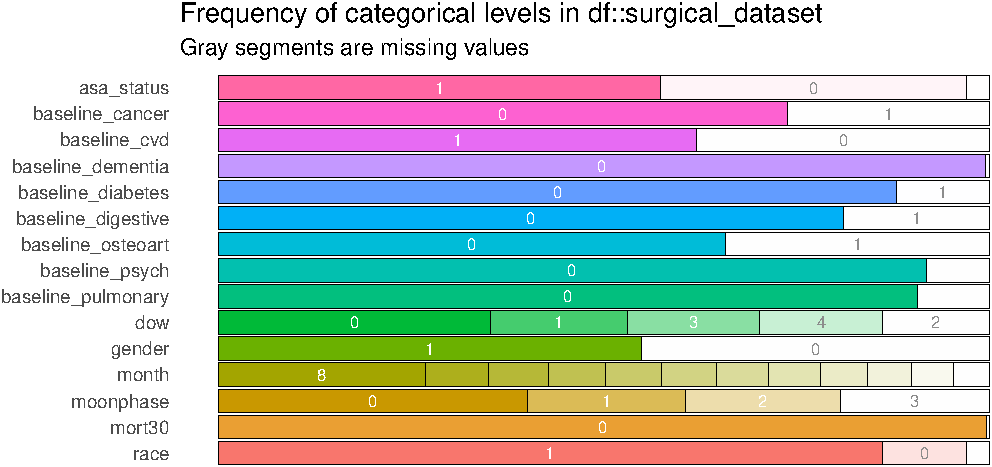
\includegraphics{memoria_files/figure-latex/unnamed-chunk-7-1}

A simple vista, prácticamente todas las categorías presentan una alta
frecuencia de aparición, \textbf{salvo por \emph{baseline\_dementia} y
\emph{mort30}}, donde el número de observaciones a 1 es de 71 y 58,
respectivamente.

\begin{Shaded}
\begin{Highlighting}[]
\NormalTok{surgical\_dataset[, }\KeywordTok{c}\NormalTok{(}\StringTok{"baseline\_dementia"}\NormalTok{, }\StringTok{"mort30"}\NormalTok{)] }\OperatorTok{\%>\%}\StringTok{ }\KeywordTok{map}\NormalTok{(table)}
\end{Highlighting}
\end{Shaded}

\begin{verbatim}
## $baseline_dementia     $mort30
##
##     0     1                0       1
## 14564    71            14577      58
\end{verbatim}

Es decir, se tratan de variables con pocas observaciones con valor 1. De
hecho, si analizamos el valor de información haciendo uso del paquete
\emph{scorecard}, la cual nos permite estudiar el ``poder predictivo de
una variable'', observamos que el valor de información es cero,
\textbf{dada la poca representatividad de los valores a 1}, de forma que
el paquete \emph{scorecard} acaba uniendo ambas categorías, lo que se
traduce en un escaso poder de predicción:

\begin{figure}[h!]

{\centering 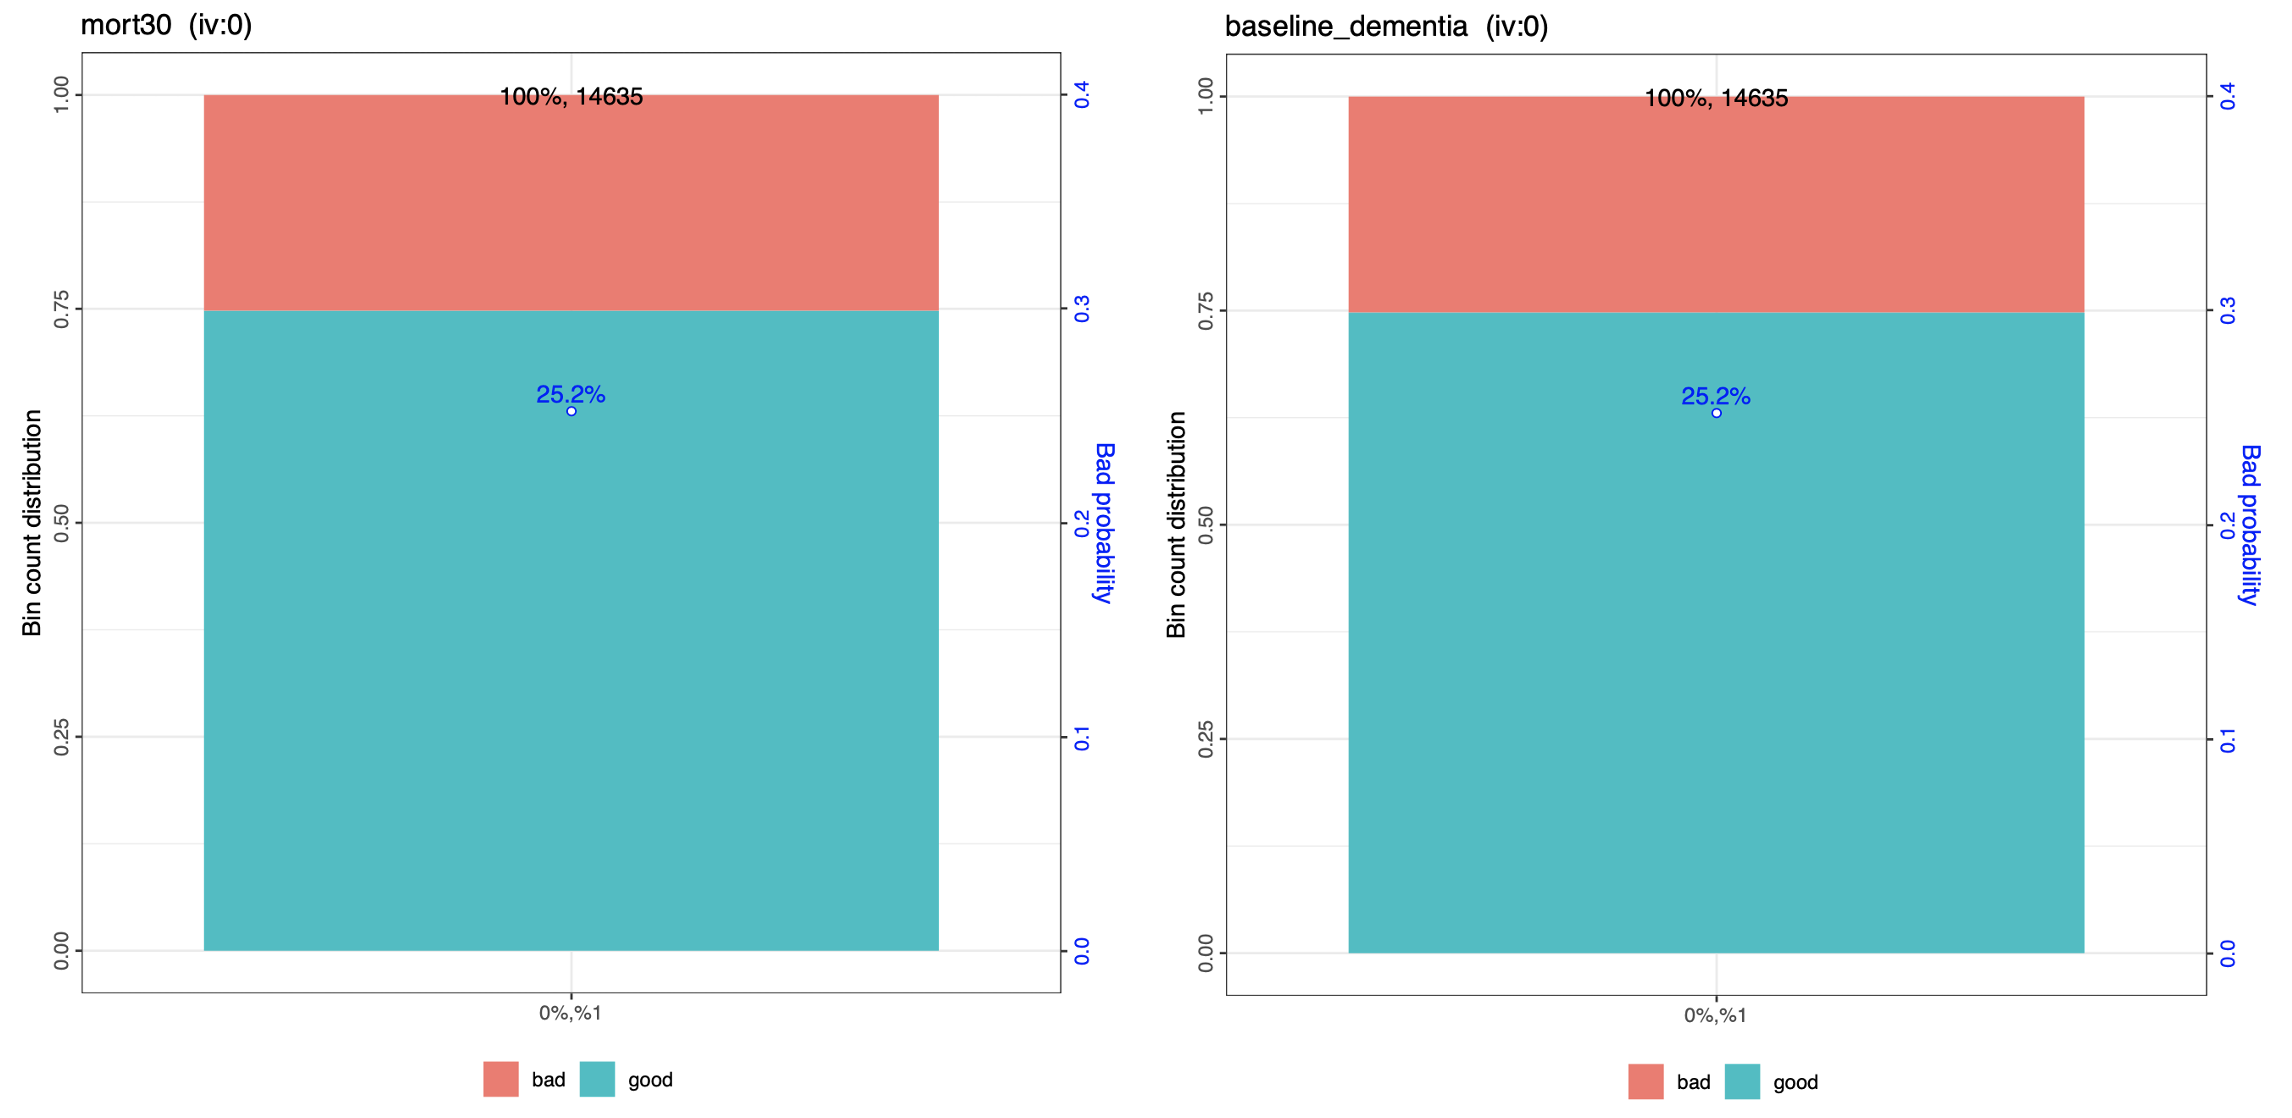
\includegraphics[width=0.99\linewidth,height=0.99\textheight,]{./capturas/Depuracion/woebin_mort30_dementia} 

}

\caption{Mort 30 y Baseline dementia (IV)}\label{fig:unnamed-chunk-9}
\end{figure}

Por otro lado, si analizamos la proporción de aparición de la variable
objetivo sobre cada categoría:

\begin{Shaded}
\begin{Highlighting}[]
\CommentTok{\#{-}{-} baseline\_dementia}
\NormalTok{surgical\_dataset }\OperatorTok{\%>\%}
\StringTok{    }\KeywordTok{count}\NormalTok{(baseline\_dementia, complication) }\OperatorTok{\%>\%}
\StringTok{    }\KeywordTok{group\_by}\NormalTok{(complication)}
\end{Highlighting}
\end{Shaded}

\begin{verbatim}
## # A tibble: 4 x 3
## # Groups:   complication [2]
##   baseline_dementia complication     n
##   <fct>             <fct>        <int>
## 1 0                 0            10913
## 2 0                 1             3651
## 3 1                 0               32
## 4 1                 1               39
\end{verbatim}

\begin{Shaded}
\begin{Highlighting}[]
\CommentTok{\#{-}{-} mort30}
\NormalTok{surgical\_dataset }\OperatorTok{\%>\%}
\StringTok{    }\KeywordTok{count}\NormalTok{(mort30, complication) }\OperatorTok{\%>\%}
\StringTok{    }\KeywordTok{group\_by}\NormalTok{(complication)}
\end{Highlighting}
\end{Shaded}

\begin{verbatim}
## # A tibble: 4 x 3
## # Groups:   complication [2]
##   mort30 complication     n
##   <fct>  <fct>        <int>
## 1 0      0            10924
## 2 0      1             3653
## 3 1      0               21
## 4 1      1               37
\end{verbatim}

A simple vista, en ambas variables \textbf{no existe una clara
separación sobre la variable objetivo}. Por tanto, se ha tomado la
decisión de descartar ambas columnas del conjunto de datos.

\begin{Shaded}
\begin{Highlighting}[]
\NormalTok{surgical\_dataset}\OperatorTok{$}\NormalTok{baseline\_dementia <{-}}\StringTok{ }\OtherTok{NULL}\NormalTok{; surgical\_dataset}\OperatorTok{$}\NormalTok{mort30 <{-}}\StringTok{ }\OtherTok{NULL} 

\CommentTok{\# Actualizamos el vector con las variables categoricas}
\NormalTok{cat\_columns <{-}}\StringTok{ }\KeywordTok{setdiff}\NormalTok{(cat\_columns, }\KeywordTok{c}\NormalTok{(}\StringTok{"baseline\_dementia"}\NormalTok{, }\StringTok{"mort30"}\NormalTok{))}
\end{Highlighting}
\end{Shaded}

\hypertarget{agrupaciuxf3n-de-variables-categuxf3ricas}{%
\subsubsection{3.3.1 Agrupación de variables
categóricas}\label{agrupaciuxf3n-de-variables-categuxf3ricas}}

Por otro lado, nos encontramos con dos variables cuyas categorías pueden
ser agrupadas, según la información proporcionada por el paquete
\emph{scorecard}:

\textbf{DÍA DE LA SEMANA} (dow):

Sobre dicha variable, \textbf{observamos una relación ``lineal'' en la
distribución de la variable objetivo a lo largo de los diferentes días
de la semana}, comenzando por el Lunes (0), con el menor porcentaje de
complicaciones hospitalarias (alrededor del 14 \%), seguido de los
Martes-Miércoles-Jueves, donde el porcentaje aumenta hasta el 30.4 \%, y
finalizando con los viernes, donde se alcanza el mayor porcentaje de
complicaciones hospitalarias: 34.5 \%:

\begin{figure}[h!]

{\centering 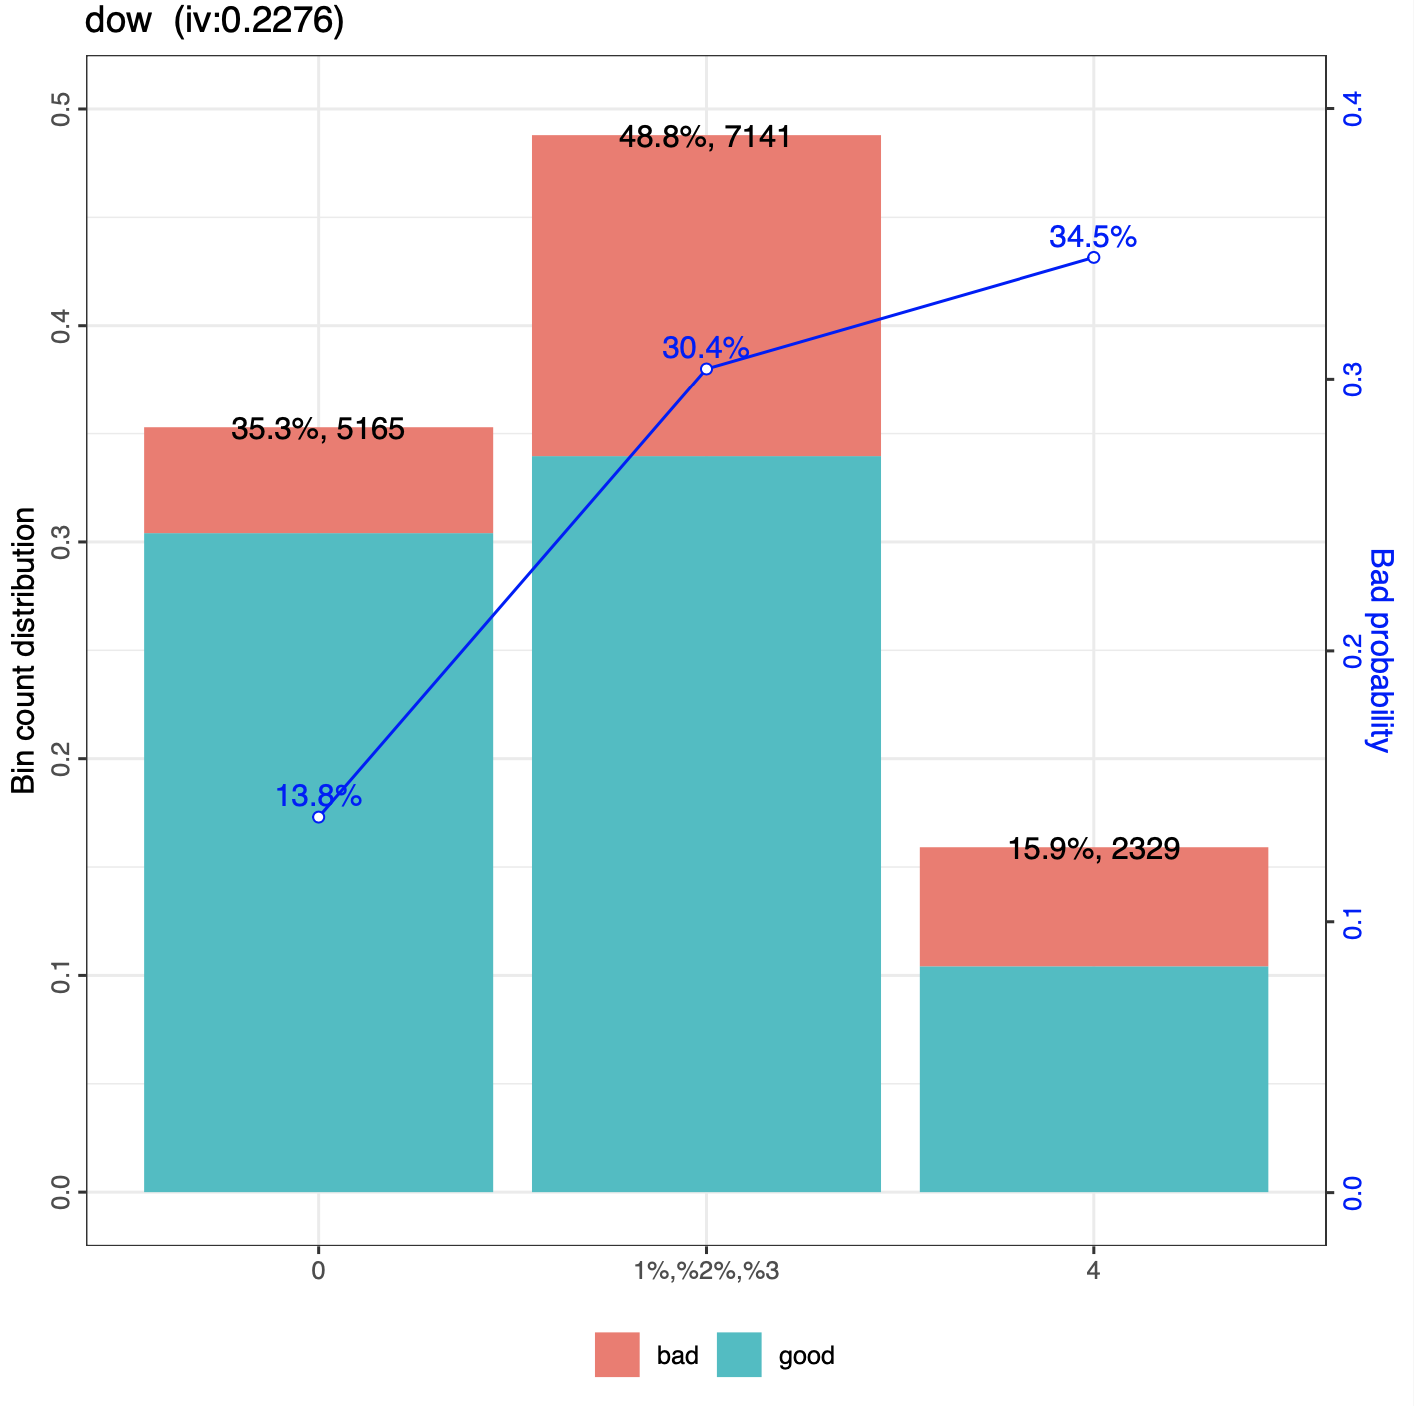
\includegraphics[width=0.65\linewidth,height=0.65\textheight,]{./capturas/Depuracion/dow} 

}

\caption{Dia de la semana o dow (IV)}\label{fig:unnamed-chunk-12}
\end{figure}

Por otro lado, si analizamos detenidamente el gráfico de distribución:

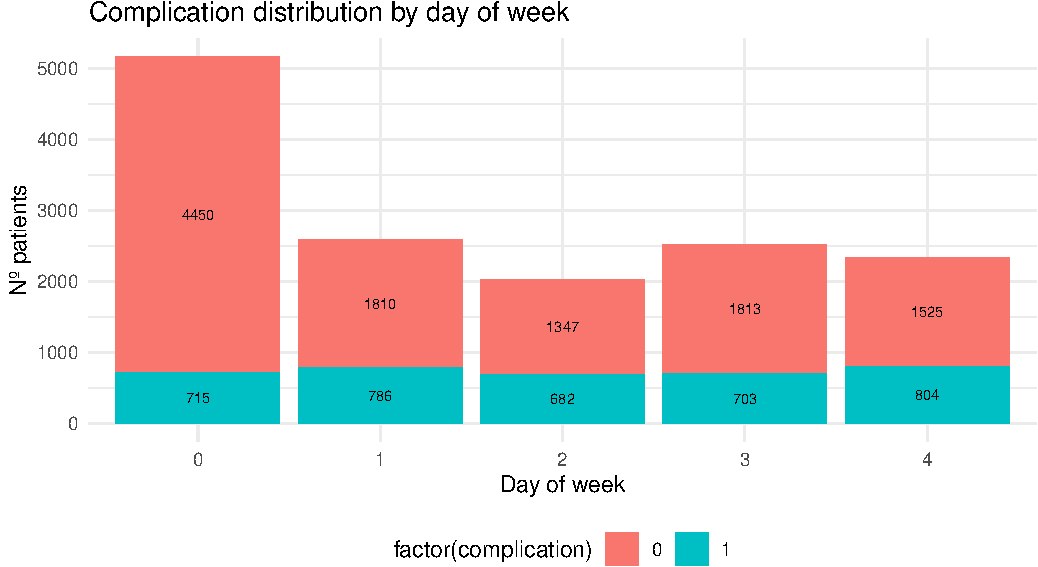
\includegraphics{memoria_files/figure-latex/unnamed-chunk-13-1}

Observamos que la proporción de aparición de pacientes con
complicaciones es muy similar entre los martes, miércoles y jueves:

\begin{verbatim}
##                   dow sin.comp con.comp total prop.complicacion
## 1                   1     4450      715  2596              30.3
## 2                   2     1810      786  2029              33.6
## 3                   3     1347      682  2516              27.9
## 4 En conjunto (1-2-3)     1813      703  7141              30.4
## 5                   4     1525      804  2329              34.5
\end{verbatim}

En conjunto, acumulan alrededor del 30.4 \% de pacientes con
complicaciones, mientras que con tan solo el viernes aumenta hasta
alcanzar el 34 \%. Por tanto, dado que los martes, miércoles y jueves
presentan una proporción de aparición similar, \textbf{las agrupamos en
torno a una misma categoría}:

\begin{enumerate}
\def\labelenumi{\arabic{enumi}.}
\tightlist
\item
  \textbf{Lunes (0)}
\item
  \textbf{Martes-Miercoles-Jueves (1-3)}
\item
  \textbf{Viernes (4)}
\end{enumerate}

\textbf{MES} (month):

\begin{figure}[h!]

{\centering 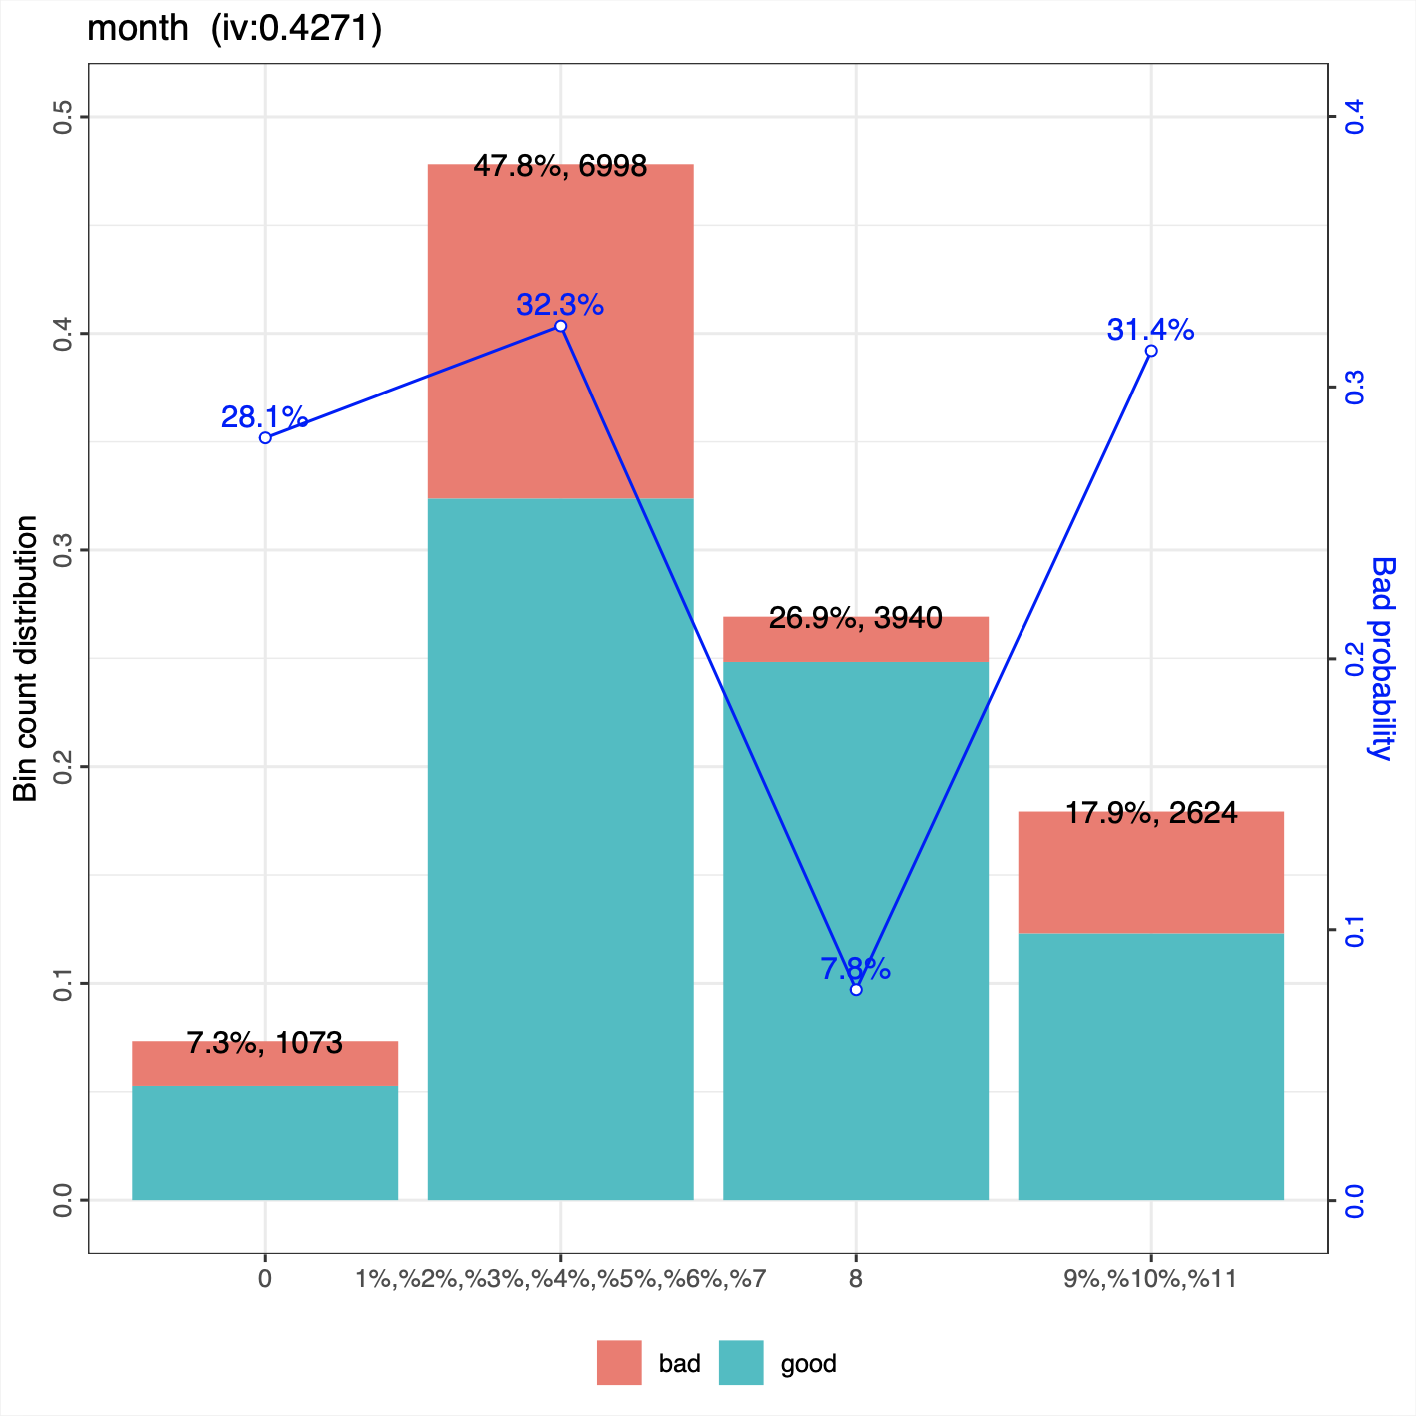
\includegraphics[width=0.75\linewidth,height=0.75\textheight,]{./capturas/Depuracion/month} 

}

\caption{Month (IV)}\label{fig:unnamed-chunk-15}
\end{figure}

En este caso, llaman la atención tres principales grupos: en primer
lugar el mes de enero (0), con un 28.1 \% de las complicaciones
hospitalarias, \textbf{seguido de los meses de febrero (1) hasta agosto
(7) con un total acumulado del 32.3 \% de los pacientes con
complicaciones}, es decir, el mes de enero tiene un porcentaje similar
de pacientes con complicaciones que los siguientes 7 meses en conjunto.
Por el contrario, \textbf{durante el mes de septiembre (8) el porcentaje
se desploma hasta el 7.8 \%}, porcentaje que vuelve a aumentar en los
tres meses siguientes (octubre, noviembre y diciembre), hasta el 31.4
\%.

Por otro lado, si analizamos el gráfico de distribución:

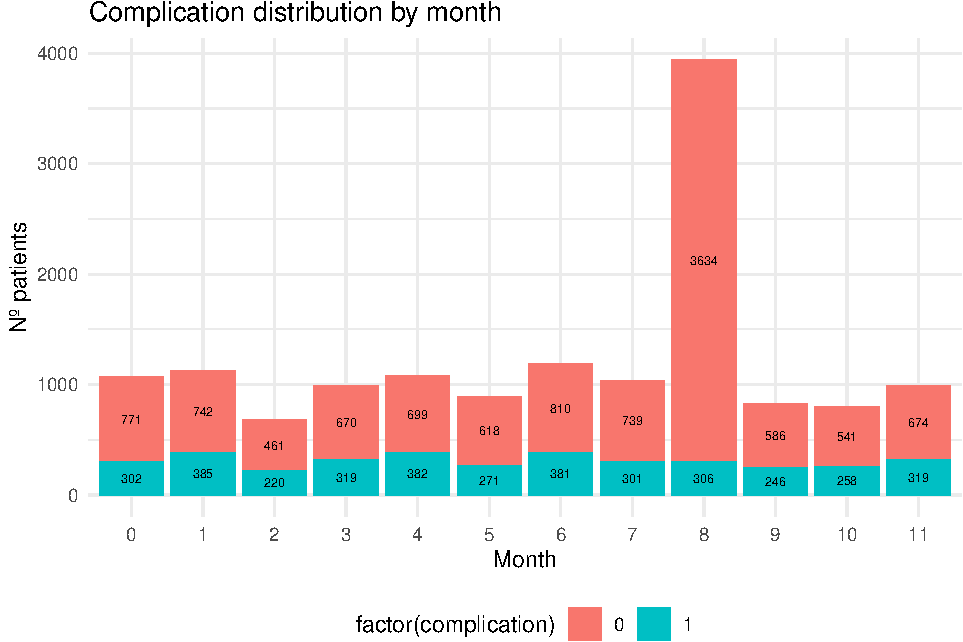
\includegraphics{memoria_files/figure-latex/unnamed-chunk-16-1}

Sucede un comportamiento similar al de la variable \emph{dow}: salvo el
mes de septiembre, \textbf{la distribución de la variable objetivo sobre
cada mes es muy similar, de forma que podemos agrupar varios de los
meses en una misma categoría, tal y como hemos comprobado
anteriormente}. A modo de ejemplo, analicemos la proporción en el número
de complicaciones hospitalarias de cada mes por separado y en conjunto:

\begin{verbatim}
##             dow sin.comp con.comp total prop.complicacion
## 1             0      771      302  1073              28.1
## 2             1      742      385  1127              34.2
## 3             2      461      220   681              32.3
## 4             3      670      319   989              32.3
## 5             4      699      382  1081              35.3
## 6             5      618      271   889              30.5
## 7             6      810      381  1191              32.0
## 8             7      739      301  1040              28.9
## 9   Uniendo 1-7     4739     2259  6998              32.3
## 10            8     3634      306  3940               7.8
## 11            9      586      246   832              29.6
## 12           10      541      258   799              32.3
## 13           11      674      319   993              32.1
## 14 Uniendo 9-11     1801      823  2624              31.4
\end{verbatim}

Como podemos comprobar, \textbf{la proporción de pacientes con
complicaciones hospitalarias, entre los meses de febrero (1) y agosto
(7), se sitúa en torno al 32 \% si agrupamos dichas categorías}. Del
mismo modo, \textbf{los meses de octubre, noviembre y diciembre (9, 10 y
11) se sitúan en torno al 31 \%}. Como consecuencia, y dado que dichas
categorías presentan una proporción similar en cuanto a pacientes con
complicaciones se refiere, las agrupamos:

\begin{enumerate}
\def\labelenumi{\arabic{enumi}.}
\tightlist
\item
  \textbf{Enero (0)}
\item
  \textbf{Febrero a Agosto (1-7)}
\item
  \textbf{Septiembre (8)}
\item
  \textbf{Octubre, Noviembre y Diciembre (9-10-11)}
\end{enumerate}

En relación con el resto de variables categóricas, si analizamos su
valor de información:

\begin{verbatim}
##              variable     iv
## 1   baseline_osteoart 0.5246
## 2               month 0.4271
## 3                 dow 0.2276
## 4           moonphase 0.2119
## 5     baseline_cancer 0.1358
## 6        baseline_cvd 0.0429
## 7              gender 0.0221
## 8  baseline_digestive 0.0134
## 9          asa_status 0.0062
## 10 baseline_pulmonary 0.0053
## 11  baseline_diabetes 0.0013
## 12               race 0.0002
## 13     baseline_psych 0.0001
\end{verbatim}

Por lo general, la mayoría de las variables categóricas presentan, como
primera impresión, un buen poder predicitivo, con ciertas excepciones
como \emph{asa\_status}, \emph{baseline\_pulmonary},
\emph{baseline\_diabetes}, \emph{race} o \emph{baseline\_pysch}, cuyo IV
no alcanza el 0.01 (como normal general, un valor de información
inferior a 0.1-0.02 se traduce en un poder predictivo muy bajo o
prácticamente nulo)\footnote{\url{https://docs.tibco.com/pub/sfire-dsc/6.5.0/doc/html/TIB_sfire-dsc_user-guide/GUID-07A78308-525A-406F-8221-9281F4E9D7CF.html}}.
De este modo, de cara a la selección de variables, \textbf{en caso de
ser necesario descartar alguna variable categórica, utilizaremos esta
tabla como referencia}.

\hypertarget{variables-continuas}{%
\subsection{3.4 Variables continuas}\label{variables-continuas}}

En relación con las variables continuas, nos encontramos con algunas
variables con un número de valores únicos muy reducidos:

\begin{Shaded}
\begin{Highlighting}[]
\CommentTok{\#{-}{-} Nº Valores unicos (continuas)}
\KeywordTok{apply}\NormalTok{(surgical\_dataset[, num\_columns], }\DecValTok{2}\NormalTok{, }\ControlFlowTok{function}\NormalTok{(x) \{}\KeywordTok{length}\NormalTok{(}\KeywordTok{unique}\NormalTok{(x))\})}
\end{Highlighting}
\end{Shaded}

\begin{verbatim}
##               bmi               Age baseline_charlson          ahrq_ccs 
##              3095               672                14                22 
##     ccsMort30Rate              hour     mortality_rsi 
##                20               725               633
\end{verbatim}

A modo de ejemplo, variables como \emph{baseline\_charlson},
\emph{ahrq\_ccs} o \emph{ccsMort30Rate} presentan 14, 22 o 20 valores
únicos, respectivamente. No obstante, se tomó la decisión de mantener
dichas variables como continuas, principalmente para facilitar la
selección de variables, evitando con ello crear nuevas variables
\emph{dummy} (una por cada categoría), utilizando con ello menos
parámetros para describir el conjunto de datos.

Por otro lado, en un primer análisis exploratorio se observó que en las
variables continuas, por lo general, \textbf{no existe una clara
separación entre ambas variables objetivo}. A modo de ejemplo,
observemos las dos siguientes variables: \emph{age} y \emph{bmi}:

\textbf{AGE}:

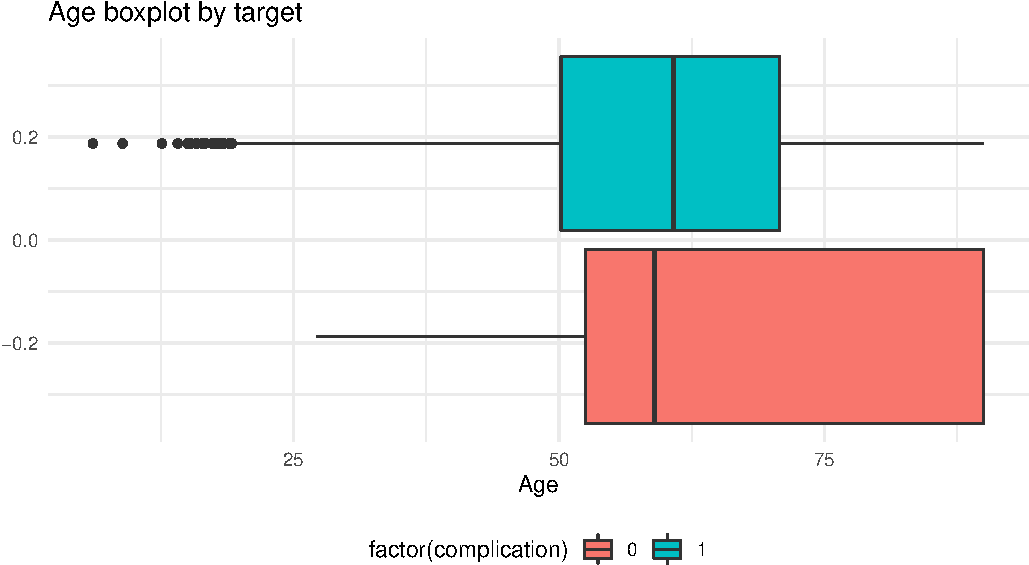
\includegraphics{memoria_files/figure-latex/unnamed-chunk-21-1}

En este caso, \textbf{bien es cierto que los pacientes que no sufren
complicaciones oscilan entre los 25 y los 90 años, aproximadamente,
mientras que existe un número de pacientes (menores a 25 años), donde
padecen alguna complicación hospitalaria}. Pese a ello, la separación no
es tan clara.

\textbf{BMI}:

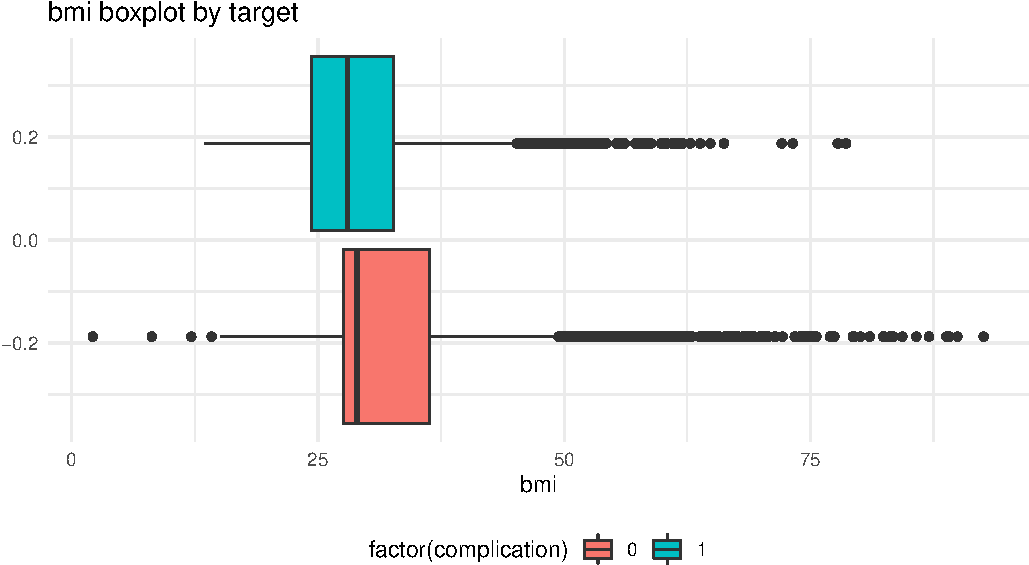
\includegraphics{memoria_files/figure-latex/unnamed-chunk-22-1}

Incluso con el índice de masa de corporal, \textbf{a simple vista no
existe una clara separación que diferencie a ambas variables objetivo en
función de dicho índice}.

\hypertarget{estandarizaciuxf3n-de-variables-continuas}{%
\subsection{3.5 Estandarización de variables
continuas}\label{estandarizaciuxf3n-de-variables-continuas}}

Una vez realizado el primer análisis, \textbf{procedemos a la
estandarización de las variables continuas}:

\begin{Shaded}
\begin{Highlighting}[]
\CommentTok{\# {-}{-}{-} Estandarizacion de variables}
\NormalTok{surgical\_dataset\_stnd <{-}}\StringTok{ }\NormalTok{surgical\_dataset}

\CommentTok{\# media}
\NormalTok{media       <{-}}\StringTok{ }\KeywordTok{sapply}\NormalTok{(surgical\_dataset\_stnd[, num\_columns], mean)}

\CommentTok{\# sd}
\NormalTok{desv.tipica <{-}}\StringTok{ }\KeywordTok{sapply}\NormalTok{(surgical\_dataset\_stnd[, num\_columns], sd)}

\NormalTok{surgical\_dataset\_stnd[, num\_columns] <{-}}\StringTok{ }\KeywordTok{scale}\NormalTok{(surgical\_dataset\_stnd[, num\_columns], }
                                              \DataTypeTok{center =}\NormalTok{ media, }
                                              \DataTypeTok{scale =}\NormalTok{ desv.tipica)}
\end{Highlighting}
\end{Shaded}

\hypertarget{creacion-de-variables-dummy}{%
\subsection{3.6 Creacion de variables
dummy}\label{creacion-de-variables-dummy}}

A continuación, convertimos las variables categóricas (con más de una
categoría) en variables \emph{dummy}, mediante la función
\emph{dummy.data.frame}, conviritiendo de este modo todas las variables
a formato numérico:

\begin{Shaded}
\begin{Highlighting}[]
\NormalTok{columnas\_dummy <{-}}\StringTok{ }\KeywordTok{c}\NormalTok{(}\StringTok{"asa\_status"}\NormalTok{, }\StringTok{"dow"}\NormalTok{, }\StringTok{"month"}\NormalTok{, }\StringTok{"moonphase"}\NormalTok{, }\StringTok{"race"}\NormalTok{)}
\NormalTok{surgical\_dataset\_stnd\_dummy <{-}}\StringTok{ }\KeywordTok{dummy.data.frame}\NormalTok{(surgical\_dataset\_stnd[, columnas\_dummy], }
                                                            \DataTypeTok{sep =} \StringTok{"."}\NormalTok{)}
\end{Highlighting}
\end{Shaded}

Una vez codificadas las variables, \textbf{comprobamos si existen
variables \emph{dummy} con una frecuencia de aparición menor a 100}:

\begin{Shaded}
\begin{Highlighting}[]
\KeywordTok{names}\NormalTok{(surgical\_dataset\_stnd\_dummy[, }\KeywordTok{colSums}\NormalTok{(surgical\_dataset\_stnd\_dummy }\OperatorTok{==}\StringTok{ }\DecValTok{0}\NormalTok{) }\OperatorTok{<}\StringTok{ }\DecValTok{100}\NormalTok{, }
                                  \DataTypeTok{drop =} \OtherTok{FALSE}\NormalTok{])}
\end{Highlighting}
\end{Shaded}

\begin{verbatim}
## character(0)
\end{verbatim}

Como podemos comprobar, todas las variables \emph{dummy} codificadas
presentan una frecuencia superior. A continuación, \textbf{unimos en un
único \emph{data.table} tanto las variables numéricas, las variables
categóricas (binarias), las variables \emph{dummy}, así como la variable
objetivo}:

\begin{Shaded}
\begin{Highlighting}[]
\NormalTok{surgical\_dataset\_final <{-}}\StringTok{ }\KeywordTok{cbind}\NormalTok{(}
\NormalTok{                                surgical\_dataset\_stnd[, num\_columns],}
\NormalTok{                                surgical\_dataset\_stnd[, cat\_columns[}\OperatorTok{!}\NormalTok{cat\_columns }\OperatorTok{\%in\%}\StringTok{ }\NormalTok{columnas\_dummy]],}
\NormalTok{                                surgical\_dataset\_stnd\_dummy,}
\NormalTok{                                surgical\_dataset\_stnd[, target]}
\NormalTok{                              )}
\end{Highlighting}
\end{Shaded}

Finalmente, de cara a la elaboración de los modelos \textbf{codificamos
la variable objetivo como ``Yes'' / ``No''}, renombrando la variable
como \emph{target}:

\begin{Shaded}
\begin{Highlighting}[]
\CommentTok{\#{-}{-} Renombramos la variable objetivo como "target"}
\KeywordTok{names}\NormalTok{(surgical\_dataset\_final)[}\DecValTok{33}\NormalTok{] <{-}}\StringTok{ "target"}

\CommentTok{\# Renombramos las columnas para adecuarlas a formulas}
\KeywordTok{names}\NormalTok{(surgical\_dataset\_final) <{-}}\StringTok{ }\KeywordTok{make.names}\NormalTok{(}\KeywordTok{names}\NormalTok{(surgical\_dataset\_final))}

\CommentTok{\# 1 {-} "Yes" ; 0 {-} "No"}
\NormalTok{surgical\_dataset\_final}\OperatorTok{$}\NormalTok{target <{-}}\StringTok{ }\KeywordTok{ifelse}\NormalTok{(}
\NormalTok{  surgical\_dataset\_final}\OperatorTok{$}\NormalTok{target }\OperatorTok{==}\StringTok{ }\DecValTok{1}\NormalTok{,}
  \StringTok{"Yes"}\NormalTok{,}
  \StringTok{"No"}
\NormalTok{)}

\NormalTok{surgical\_dataset\_final}\OperatorTok{$}\NormalTok{target <{-}}\StringTok{ }\KeywordTok{as.factor}\NormalTok{(surgical\_dataset\_final}\OperatorTok{$}\NormalTok{target)}
\end{Highlighting}
\end{Shaded}

\begin{verbatim}
## Numero de variables finales (dummies incluidas):  32
\end{verbatim}

\hypertarget{selecciuxf3n-de-variables-bajo-loguxedstica}{%
\section{4. Selección de variables bajo
logística}\label{selecciuxf3n-de-variables-bajo-loguxedstica}}

\hypertarget{selecciuxf3n-de-una-submuestra}{%
\subsection{4.1 Selección de una
submuestra}\label{selecciuxf3n-de-una-submuestra}}

Durante la selección de variables, e incluso con determinados modelos
como redes neuronales o SVM, el tiempo de cómputo que requiere era
demasiado elevado. Como consecuencia, se planteó utilizar, en lugar del
\emph{dataset} completo con 14.000 observaciones, \textbf{un subconjunto
de menor tamaño}. Dado que la variable objetivo se encuentra
desbalanceada, como pudimos comprobar en el apartado de Depuración,
recurrimos al \textbf{muestreo estratificado}, el cual nos asegura la
proporción de la variable objetivo. Para ello, \emph{caret} dispone de
la función \emph{createDataPartition}, con el que obtener una submuestra
estratificada. Concretamente, para el desarrollo del proyecto empleamos
un subconjunto con el \textbf{40 \% de las observaciones}:

\begin{Shaded}
\begin{Highlighting}[]
\CommentTok{\#{-}{-} Muestreo estratificado}
\KeywordTok{set.seed}\NormalTok{(}\DecValTok{1234}\NormalTok{)}
\NormalTok{partitions <{-}}\StringTok{ }\KeywordTok{createDataPartition}\NormalTok{(surgical\_dataset\_final}\OperatorTok{$}\NormalTok{target, }\DataTypeTok{p =} \FloatTok{0.40}\NormalTok{, }\DataTypeTok{list =} \OtherTok{FALSE}\NormalTok{)}

\NormalTok{surgical\_dataset\_final\_est <{-}}\StringTok{ }\NormalTok{surgical\_dataset\_final[partitions, ]}

\CommentTok{\# Mantenemos la misma proporcion en la variable objetivo}
\KeywordTok{table}\NormalTok{(surgical\_dataset\_final\_est}\OperatorTok{$}\NormalTok{target)}
\end{Highlighting}
\end{Shaded}

\begin{verbatim}
## 
##   No  Yes 
## 4378 1476
\end{verbatim}

No obstante, con un 40 \% de los datos ¿Es suficiente? Más importante
aún ¿Se obtienen los mismos resultados o similares? Es decir, si nos
fijamos en la depuración final, nos encontramos con 14.635 / 32
\textasciitilde{} 457 observaciones por variable, aproximadamente. Sin
embargo, con tan solo el 40 \%, obtendríamos (14.635 * 0.4) / 32
\textasciitilde{} 183 observaciones por variable. Es decir, con una
menor proporción de observaciones por variable, es posible que los
modelos no sean exactamente iguales con ambos conjuntos.

Por ello, durante la selección de variables \textbf{aplicaremos las
mismas técnicas sobre ambos conjuntos}:

\begin{enumerate}
\def\labelenumi{\arabic{enumi}.}
\tightlist
\item
  \emph{stepwise AIC}
\item
  \emph{stepwise BIC}
\item
  \emph{RFE o \emph{Recursive Feature Elimination} (sobre logística)}
\item
  \emph{RFE (sobre \emph{Random Forest})}
\end{enumerate}

A continuación, y en caso de obtener una selección de variables similar,
aplicamos un modelo logístico en ambos casos, comprobando de este modo
si los resultados son similares, incluso con tan solo el 40 \% de las
observaciones. De ser así, de cara al resto de modelos trabajaremos con
el subconjunto.

\hypertarget{stepwise-aic}{%
\subsection{4.2 Stepwise AIC}\label{stepwise-aic}}

Comenzamos con la selección de variables bajo \emph{stepwise AIC}:

\begin{Shaded}
\begin{Highlighting}[]
\CommentTok{\#{-}{-} Stepwise AIC (100 repeticiones)}
\NormalTok{lista.variables.aic <{-}}\StringTok{ }\KeywordTok{steprepetidobinaria}\NormalTok{(}\DataTypeTok{data=}\NormalTok{surgical\_dataset,}
                                           \DataTypeTok{vardep=}\NormalTok{target,}\DataTypeTok{listconti=}\NormalTok{vars,}
                                           \DataTypeTok{sinicio=}\DecValTok{1234}\NormalTok{,}\DataTypeTok{sfinal=}\DecValTok{1334}\NormalTok{,}
                                           \DataTypeTok{porcen=}\FloatTok{0.8}\NormalTok{,}\DataTypeTok{criterio=}\StringTok{"AIC"}\NormalTok{)}
\NormalTok{tabla.aic <{-}}\StringTok{ }\NormalTok{lista.variables.aic[[}\DecValTok{1}\NormalTok{]]}
\end{Highlighting}
\end{Shaded}

\begin{verbatim}
##     n varible_dataset_original   variable_subset
## 1   1            mortality_rsi     mortality_rsi
## 2   2            ccsMort30Rate     ccsMort30Rate
## 3   3                      bmi               bmi
## 4   4                  month.8           month.8
## 5   5             baseline_cvd      baseline_cvd
## 6   6                    dow.0             dow.0
## 7   7                      Age               Age
## 8   8              moonphase.0       moonphase.0
## 9   9                  month.0           month.0
## 10 10             asa_status.0      asa_status.0
## 11 11        baseline_osteoart baseline_osteoart
## 12 12        baseline_charlson baseline_charlson
## 13 13                 ahrq_ccs          ahrq_ccs
## 14 14        baseline_diabetes baseline_diabetes
## 15 15          baseline_cancer                 -
## 16 16           baseline_psych                 -
## 17 17             asa_status.1                 -
\end{verbatim}

Como podemos observar, \textbf{la diferencia entre el \emph{dataset}
original y la submuestra es de tan solo 3 variables:
\emph{baseline\_cancer}, \emph{baseline\_psych} y \emph{asa\_status.1}}.

\hypertarget{stepwise-bic}{%
\subsection{4.3 Stepwise BIC}\label{stepwise-bic}}

Por otro lado, analicemos la selección de variables bajo \emph{stepwise
BIC}:

\begin{Shaded}
\begin{Highlighting}[]
\CommentTok{\#{-}{-} Stepwise BIC (100 repeticiones)}
\NormalTok{lista.variables.bic <{-}}\StringTok{ }\KeywordTok{steprepetidobinaria}\NormalTok{(}\DataTypeTok{data=}\NormalTok{surgical\_dataset,}
                                           \DataTypeTok{vardep=}\NormalTok{target,}\DataTypeTok{listconti=}\NormalTok{vars,}
                                           \DataTypeTok{sinicio=}\DecValTok{1234}\NormalTok{,}\DataTypeTok{sfinal=}\DecValTok{1334}\NormalTok{,}
                                           \DataTypeTok{porcen=}\FloatTok{0.8}\NormalTok{,}\DataTypeTok{criterio=}\StringTok{"BIC"}\NormalTok{)}
\NormalTok{tabla.bic <{-}}\StringTok{ }\NormalTok{lista.variables.bic[[}\DecValTok{1}\NormalTok{]]}
\end{Highlighting}
\end{Shaded}

\begin{verbatim}
##     n varible_dataset_original   variable_subset
## 1   1            mortality_rsi     mortality_rsi
## 2   2            ccsMort30Rate     ccsMort30Rate
## 3   3                      bmi               bmi
## 4   4                  month.8           month.8
## 5   5                    dow.0             dow.0
## 6   6                      Age               Age
## 7   7              moonphase.0       moonphase.0
## 8   8        baseline_osteoart baseline_osteoart
## 9   9             asa_status.0      asa_status.0
## 10 10          baseline_cancer                 -
\end{verbatim}

En este caso, la diferencia en ambas seleciones es de tan solo una única
variable: \emph{baseline\_cancer}.

\hypertarget{recursive-feature-elimination-bajo-loguxedstica}{%
\subsection{4.4 Recursive Feature Elimination (bajo
logística)}\label{recursive-feature-elimination-bajo-loguxedstica}}

No obstante, en ambas seleccio fnes de variables el número de parámetros
es bastante elevado, en especial con \emph{stepwise AIC}. Como
consecuencia, a los métodos anteriores añadimos una selección de
variables mediante \emph{Recursive Feature Elimination}, tanto bajo
logística como con \emph{Random Forest}:

\begin{figure}[h!]

{\centering 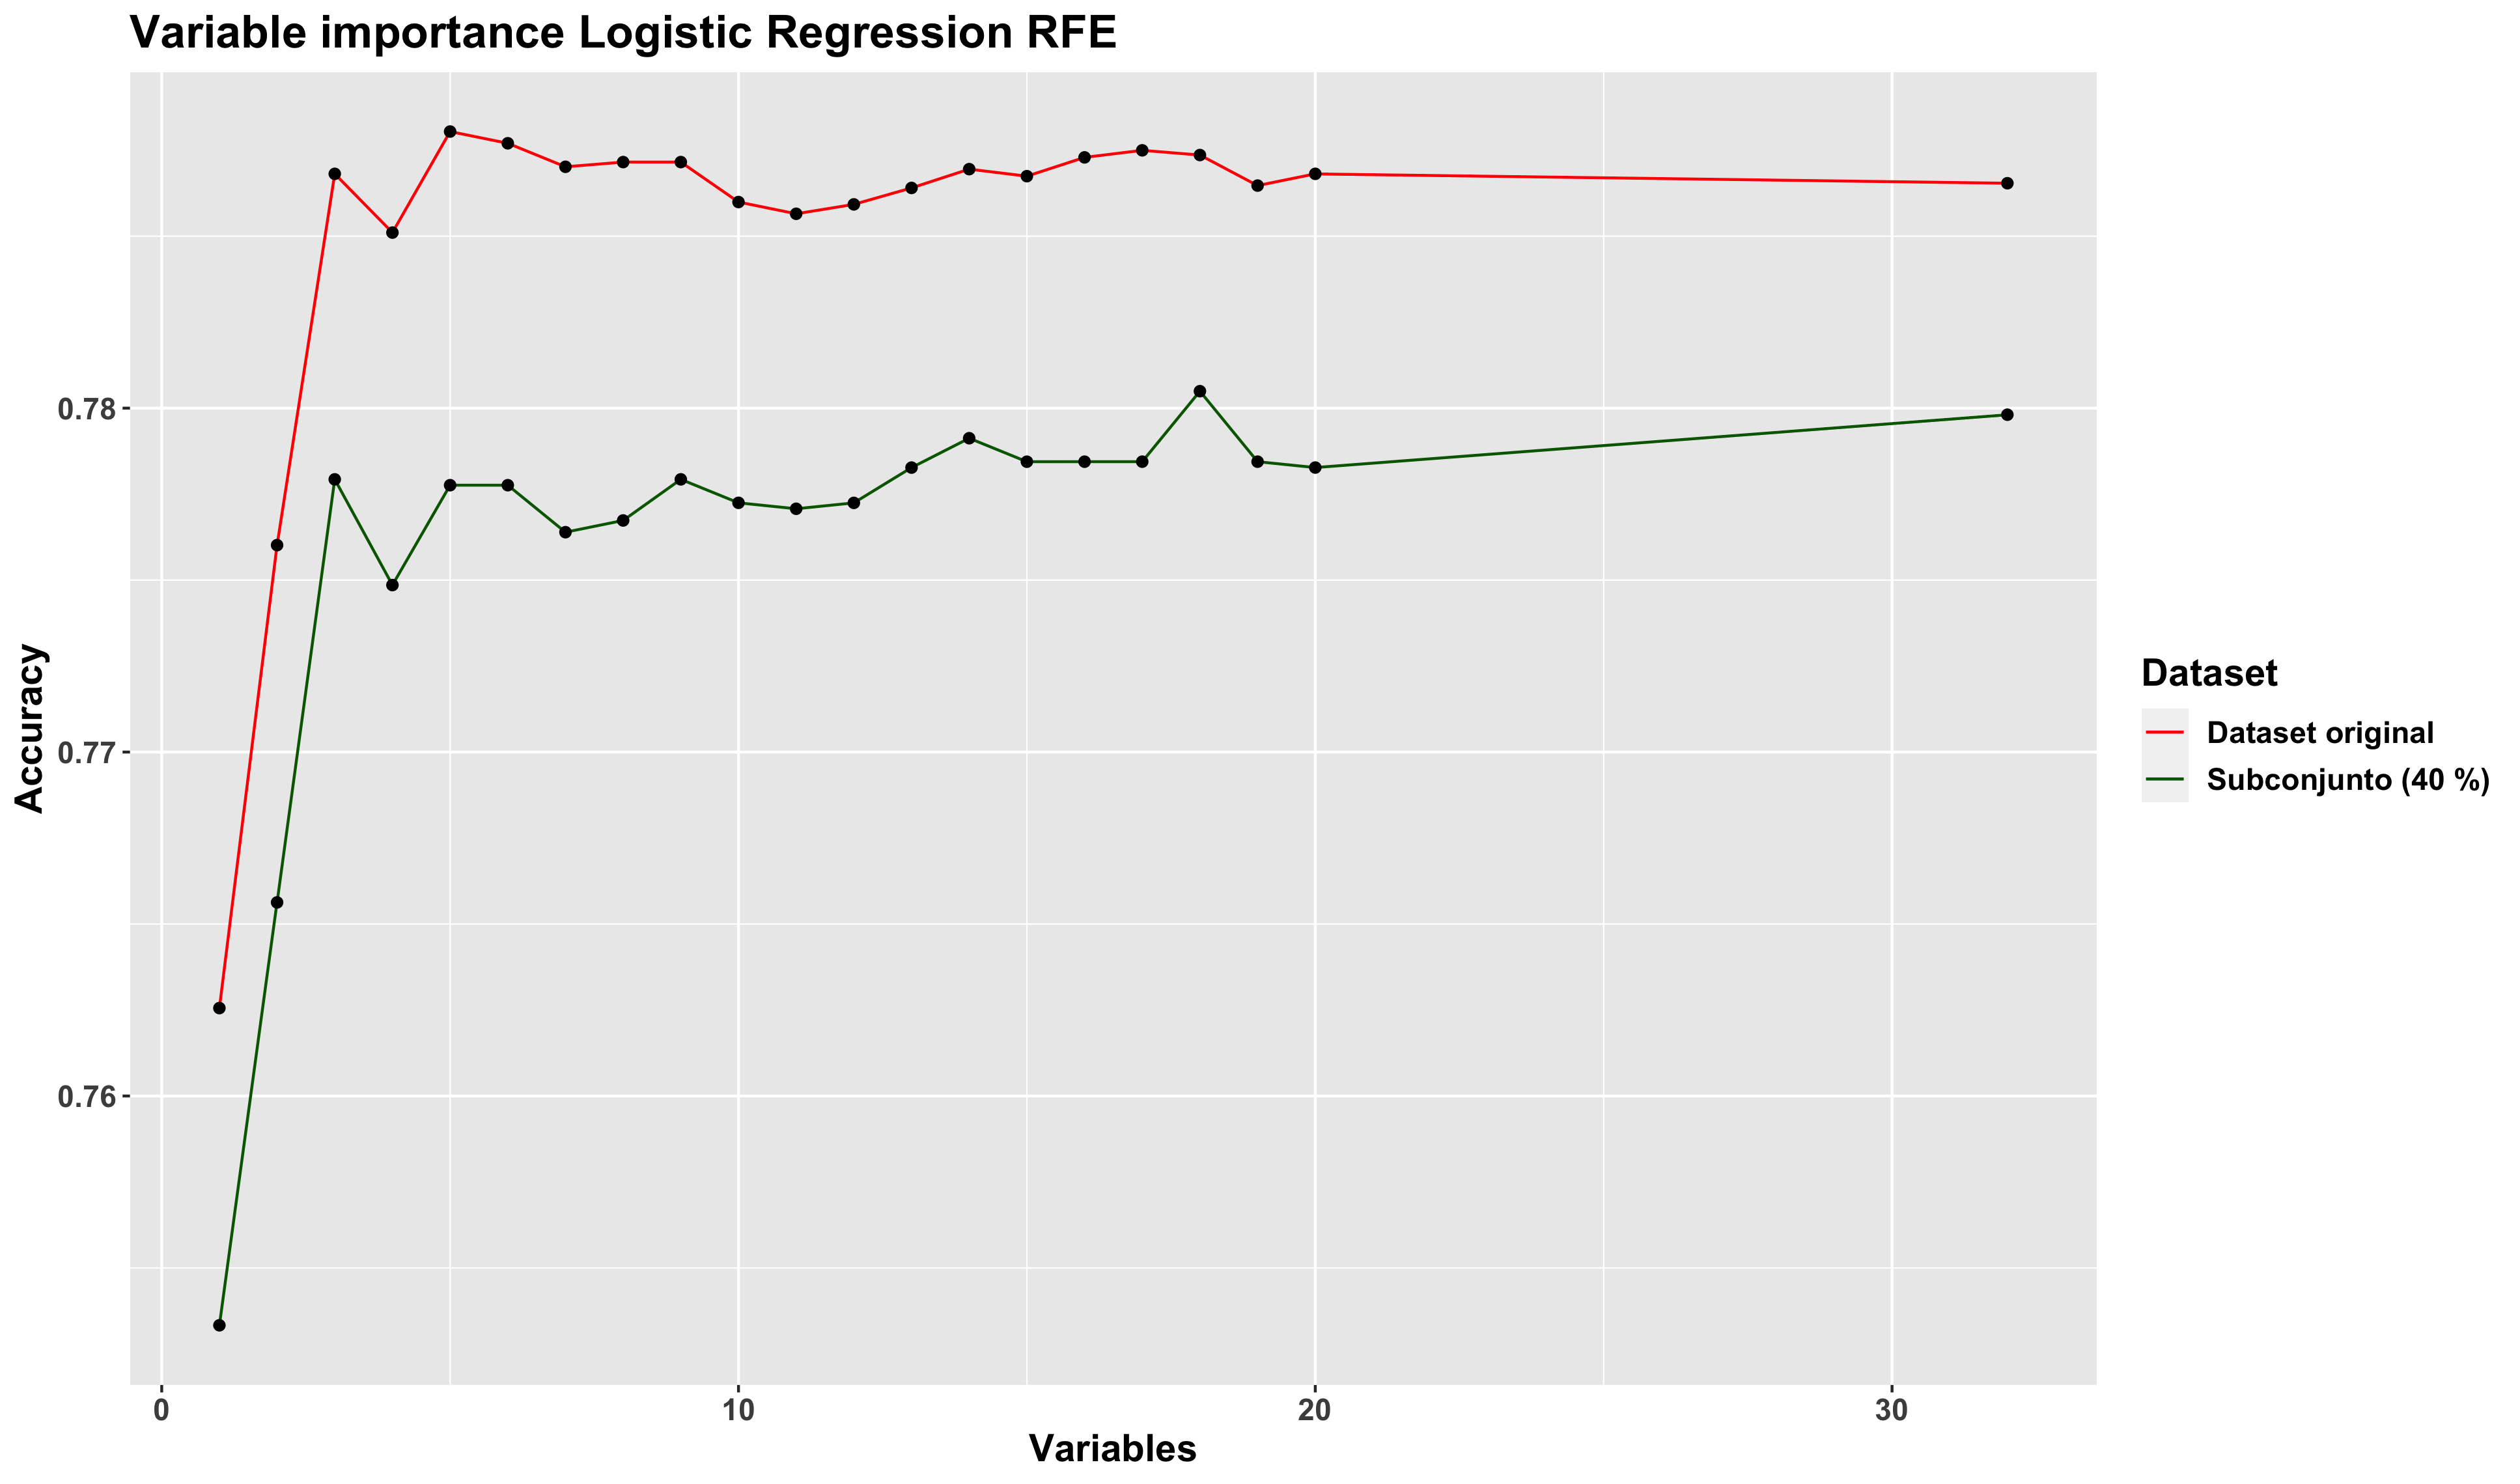
\includegraphics[width=0.99\linewidth,height=0.99\textheight,]{./charts/01_feature_selection_RFE_LR_whole_dataset} 

}

\caption{RFE Logistic Regression}\label{fig:unnamed-chunk-34}
\end{figure}

Analizando el gráfico resultante, observamos que la diferencia de
\emph{Accuracy} en ambos \emph{datasets} no es muy significativa:
\textbf{mientras que con el \emph{dataset} completo se alcanza un valor
en torno a 0.78, con el subconjunto la precisión se reduce a tan solo
0.77}. De hecho, en ambos casos se obtienen muy buenos resultados con
tan solo tres variables, y en ambos casos coinciden:

\begin{verbatim}
## Top 3 variables:

## [1] ccsMort30Rate
## [2] mortality_rsi
## [3] bmi
\end{verbatim}

\hypertarget{recursive-feature-elimination-bajo-random-forest}{%
\subsection{4.5 Recursive Feature Elimination (bajo Random
Forest)}\label{recursive-feature-elimination-bajo-random-forest}}

En el caso de \emph{Random Forest}, \textbf{con 4-5 parámetros se
obtienen resultados muy similares}: en el caso el \emph{dataset}
original en torno a 0.90 y 0.88 el caso del subconjunto. De hecho, en el
punto de máximo \emph{accuracy}, ambos modelos comparten las mismas
variables, a excepción de \emph{ahrq\_ccs}:

\begin{verbatim}
##   n varible_dataset_original variable_subset
## 1 1                      Age             Age
## 2 2            ccsMort30Rate   ccsMort30Rate
## 3 3            mortality_rsi   mortality_rsi
## 4 4                      bmi             bmi
## 5 5                        -        ahrq_ccs
\end{verbatim}

\newpage
\begin{figure}[h!]

{\centering 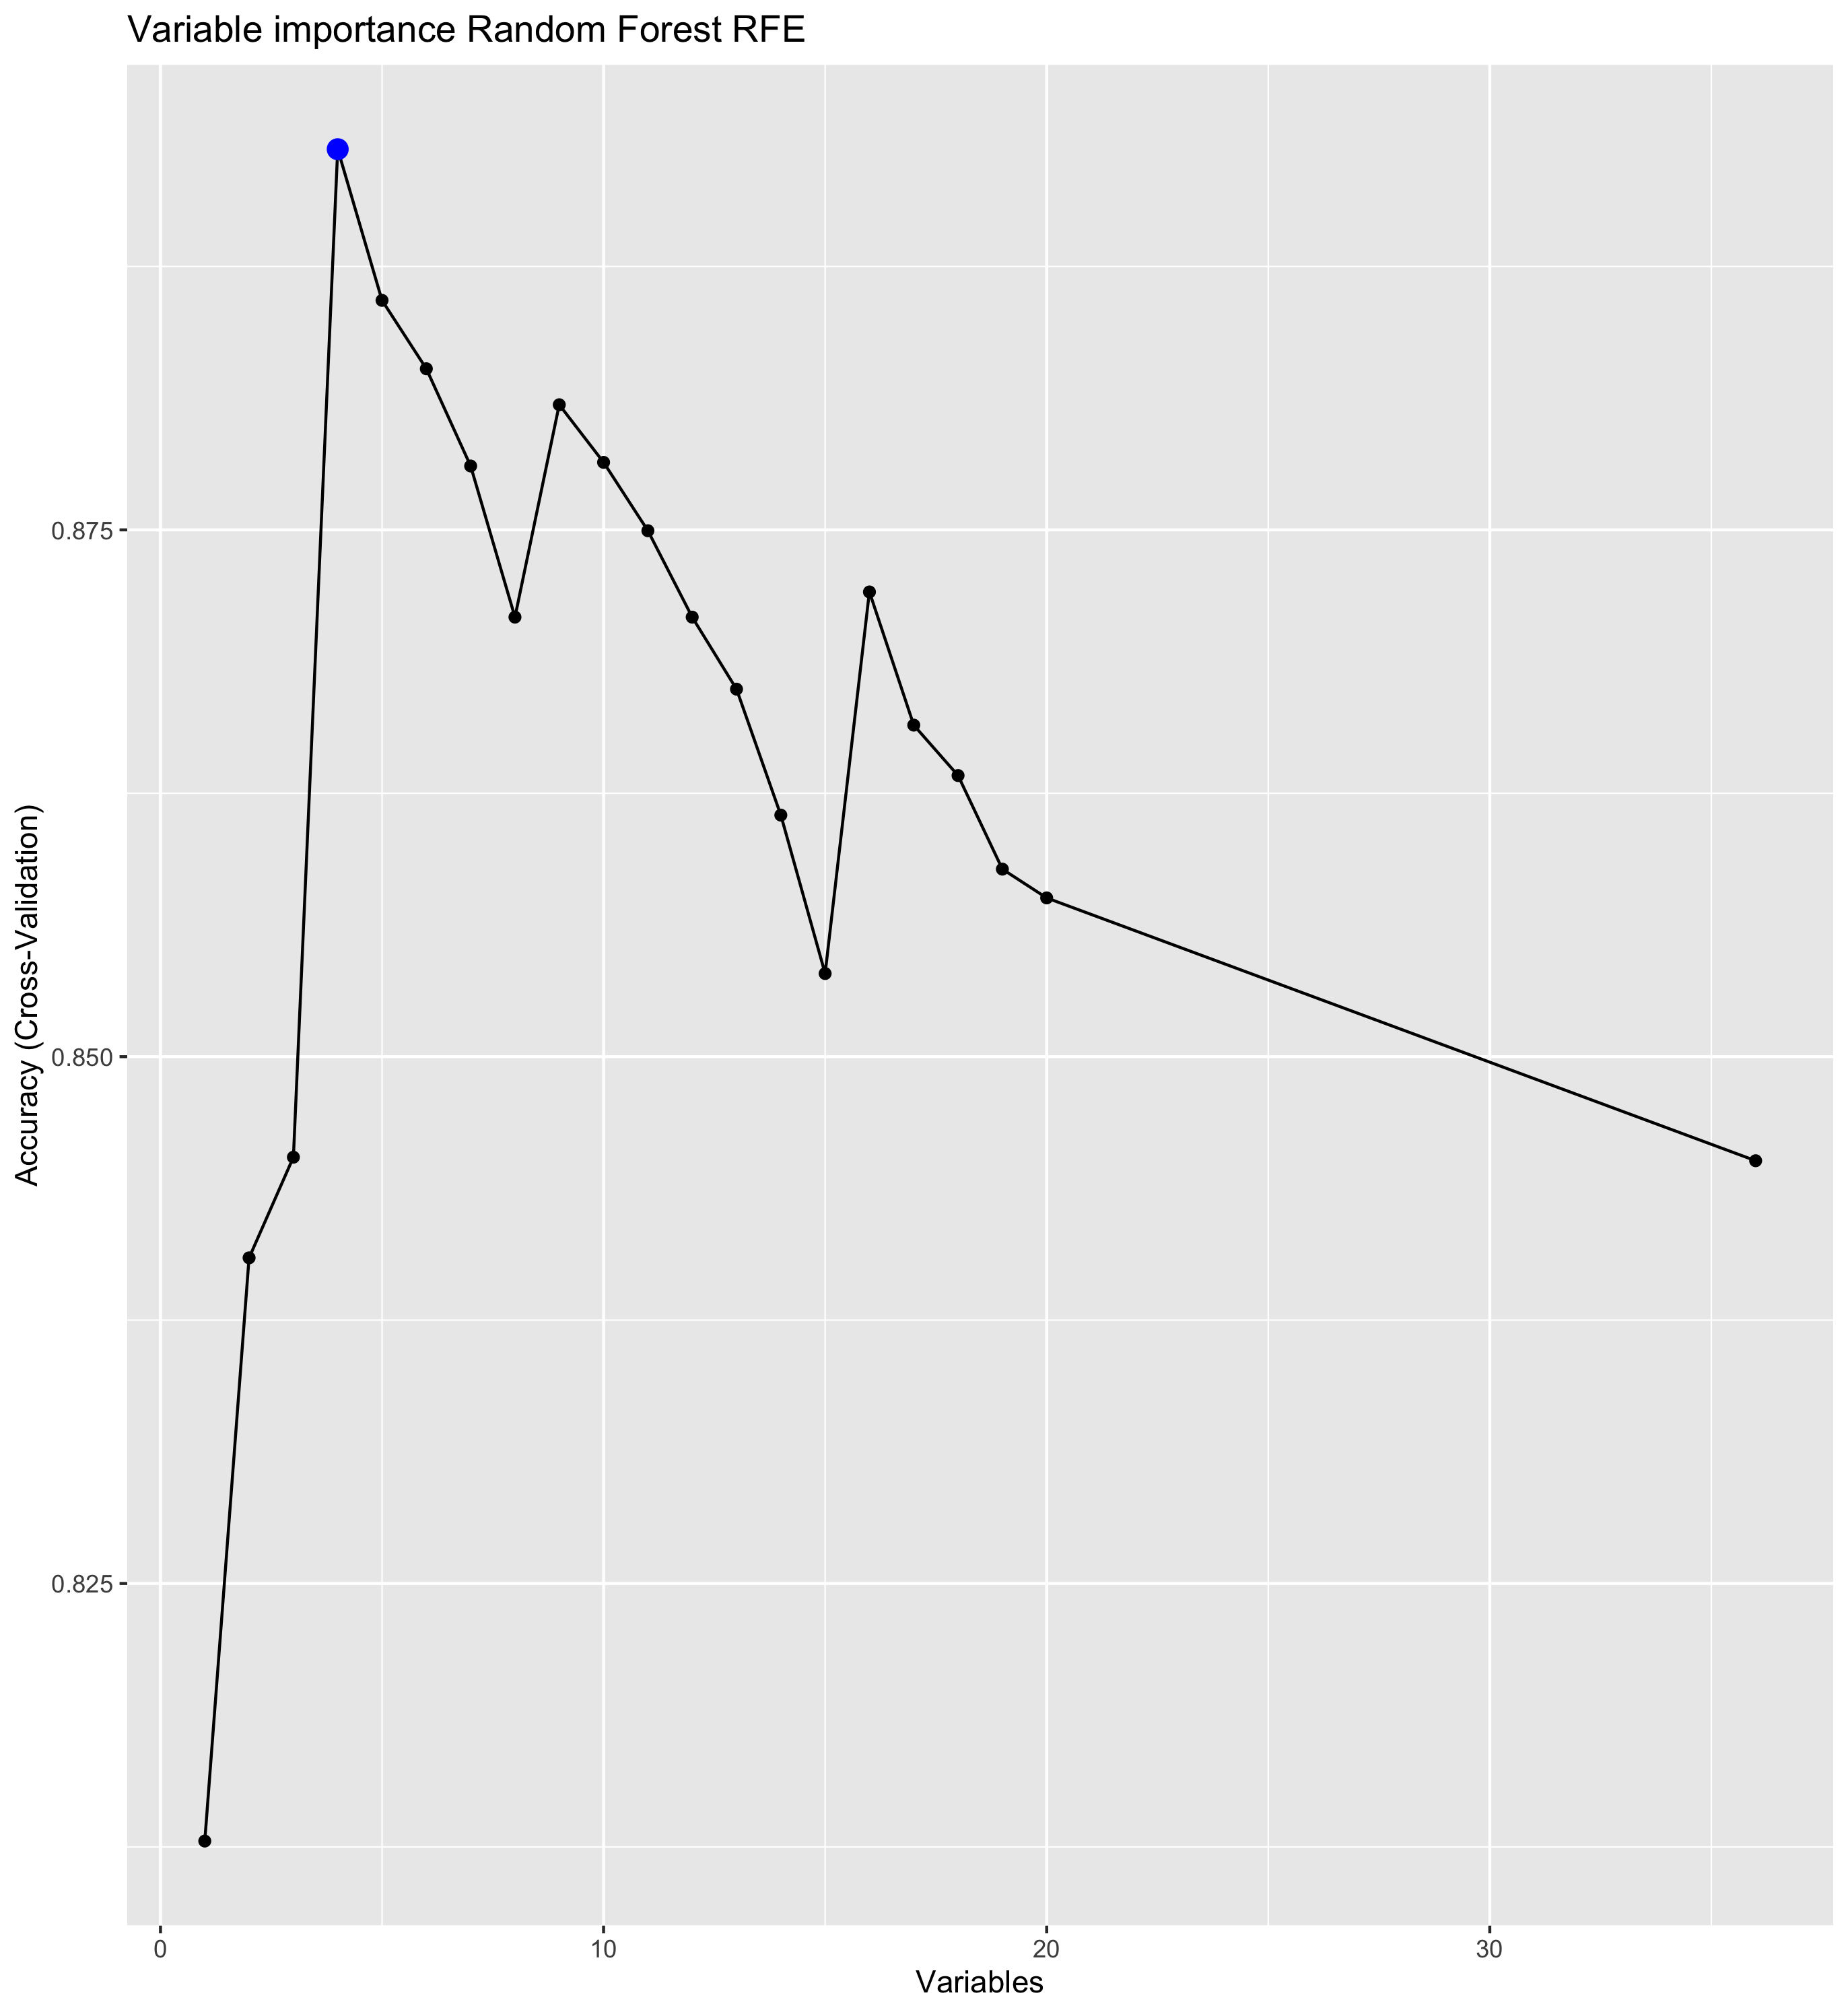
\includegraphics[width=0.99\linewidth,height=0.99\textheight,]{./charts/01_feature_selection_RFE_RF_whole_dataset} 

}

\caption{RFE Random Forest}\label{fig:unnamed-chunk-36}
\end{figure}

\hypertarget{selecciuxf3n-bajo-loguxedstica}{%
\subsection{4.6 Selección bajo
logística}\label{selecciuxf3n-bajo-loguxedstica}}

\hypertarget{comparaciuxf3n-datasets}{%
\subsubsection{4.6.1 Comparación
datasets}\label{comparaciuxf3n-datasets}}

A continuación, y una vez realizada la selección de variables tanto por
AIC/BIC como por RFE, \textbf{realizamos una primera comparación, bajo
logística, de la selección de variables obtenidas en los métodos
anteriores, tanto con el \emph{dataset} original como con el
subconjunto}:

\begin{figure}[h!]

{\centering 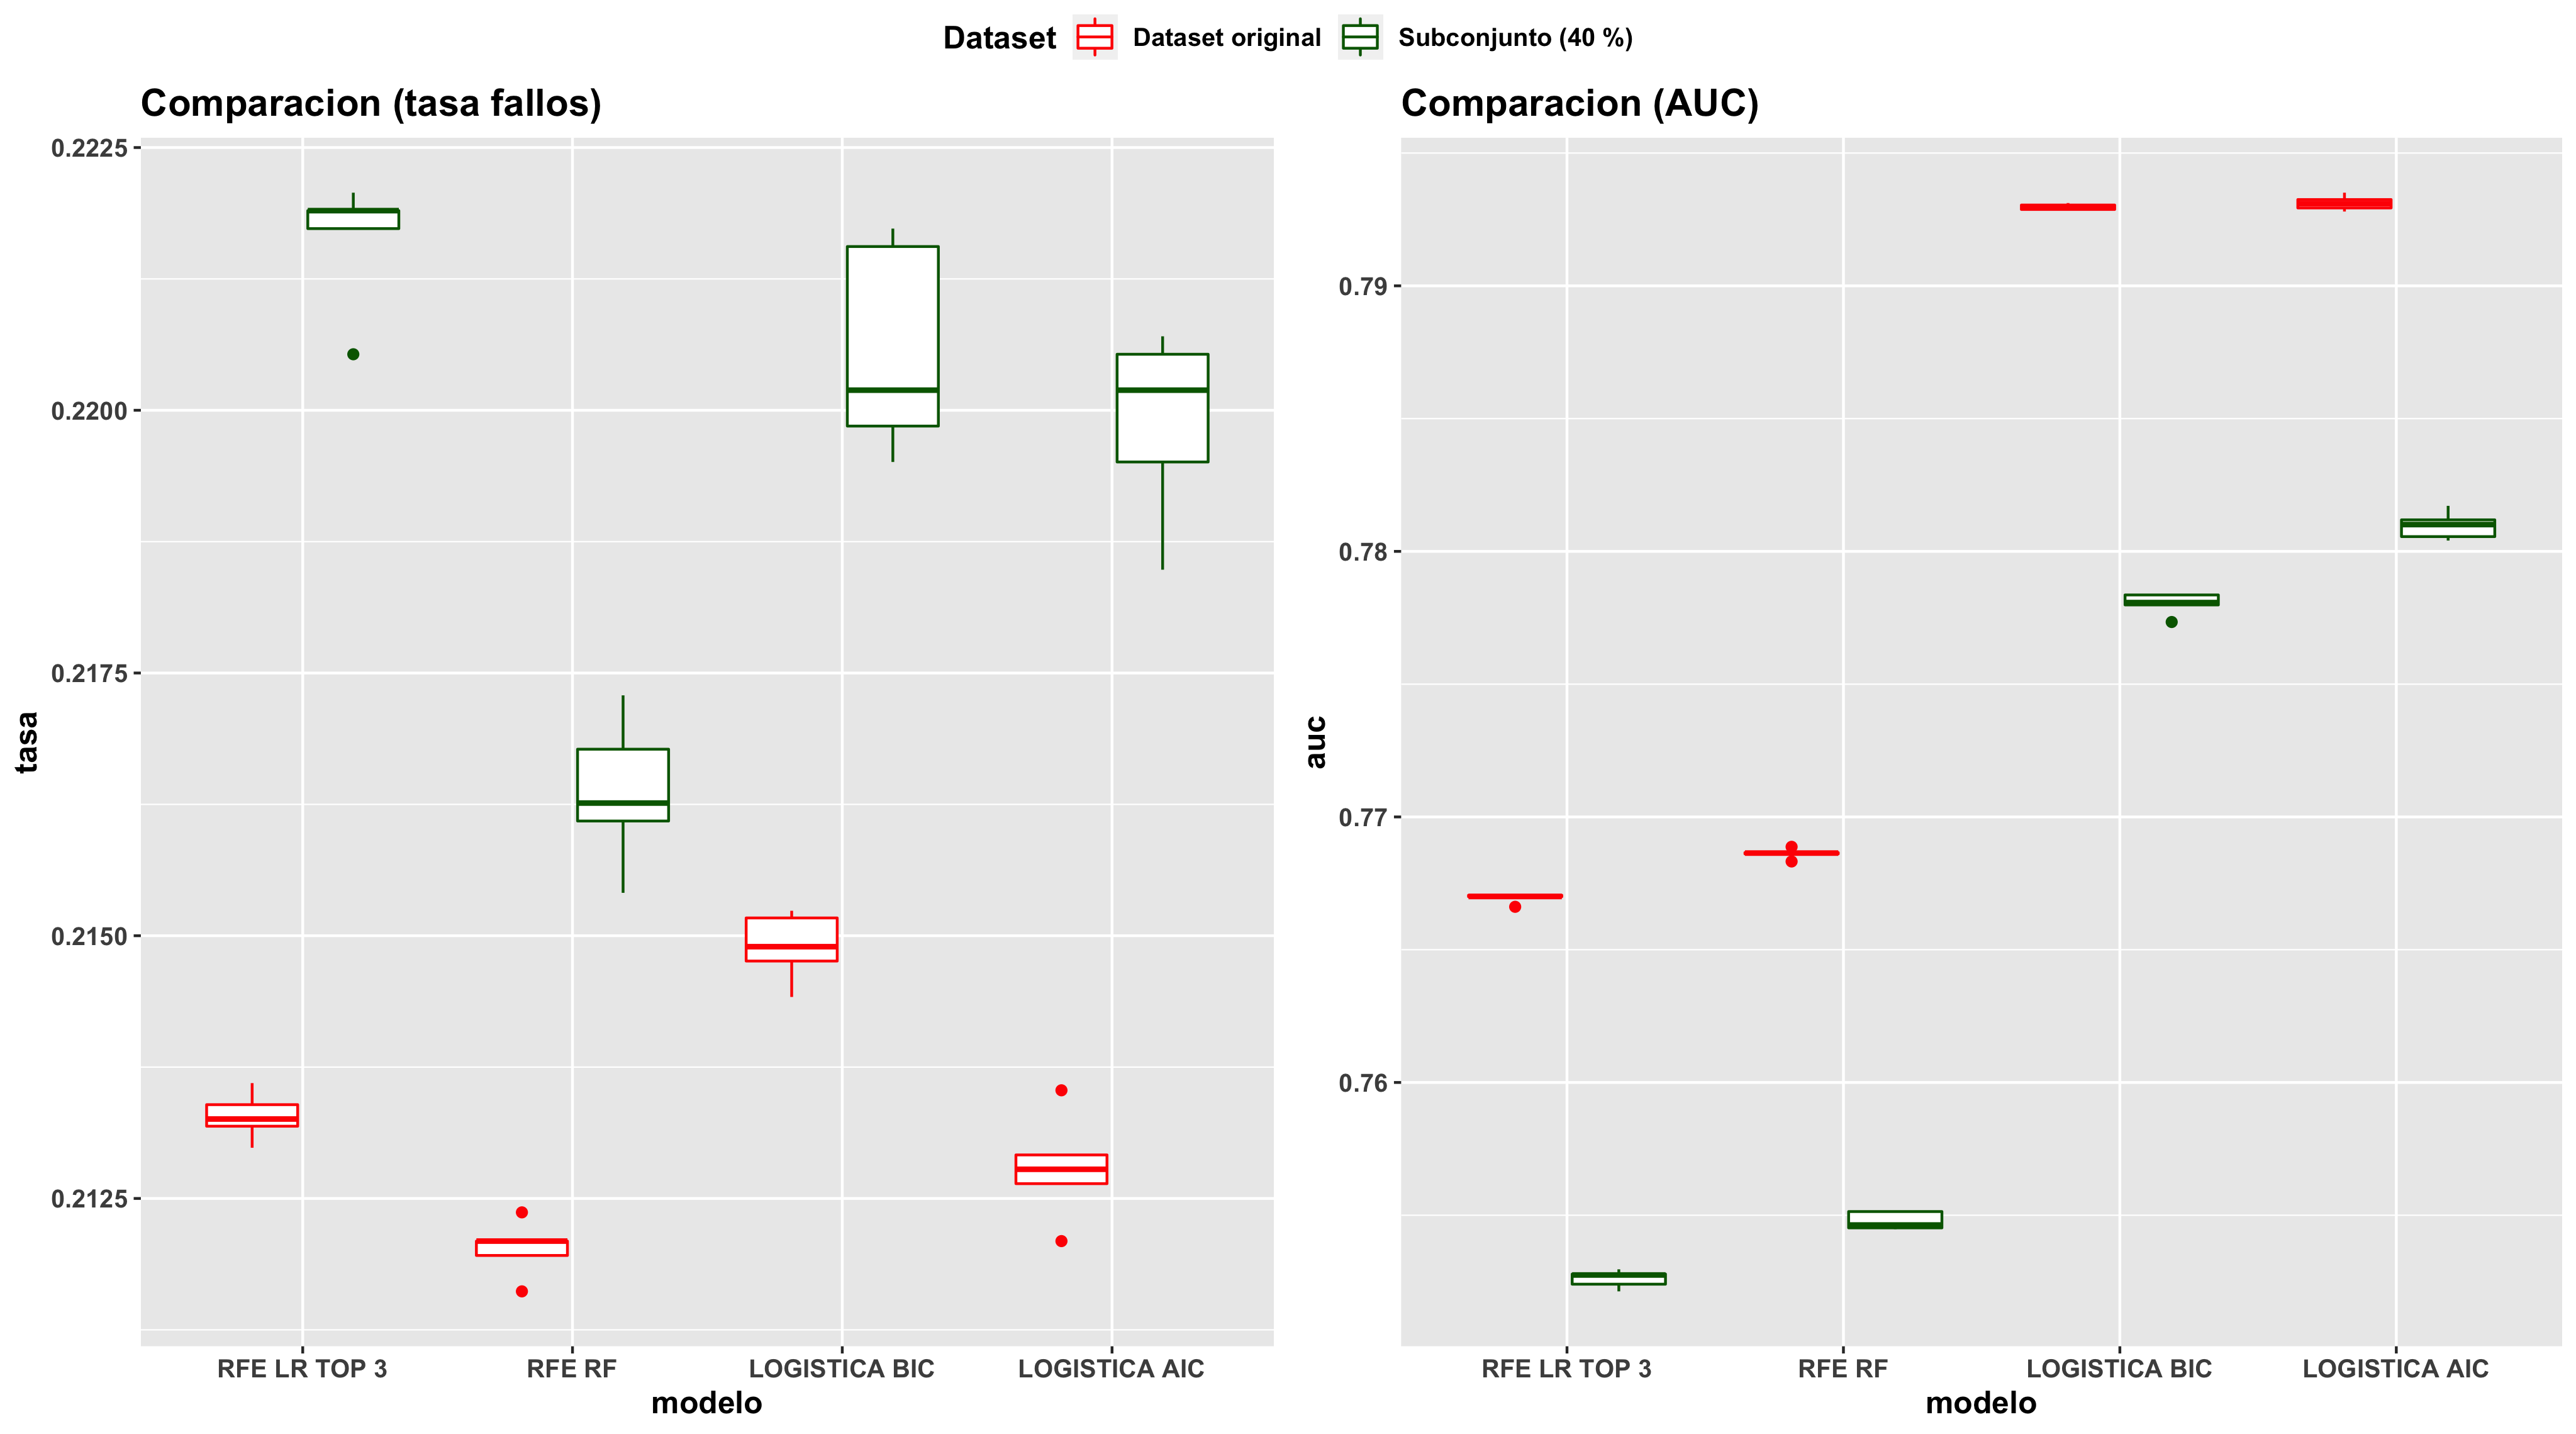
\includegraphics[width=0.99\linewidth,height=0.99\textheight,]{./charts/01_feature_selection_primera_comparacion} 

}

\caption{Comparacion bajo logística (I)}\label{fig:unnamed-chunk-37}
\end{figure}

Como primera impresión, y dada la escala del eje Y, la diferencia en
cuanto a tasa de fallos y AUC se refiere es muy pequeña, concretamente
de 0.01, aproximadamente (0.21 en tasa de fallos y 0.79 en AUC frente a
0.22 y 0.78).

Por tanto, dado que la diferencia entre ambos \emph{datasets} es
pequeña, \textbf{de cara al resto de la práctica se trabajó con el
subconjunto del 40 \%}. No obstante, en los últimos apartados (y una vez
tuneados los modelos), se realiza una última comparación con el fichero
original, comprobando de este modo si el orden de los algoritmos se
conserva. Además, de cara a la evaluación de los modelos se ha tomado la
decisión de utilizar el resto de observaciones del \emph{dataset}
original como conjunto \emph{test} \textbf{con el que evaluar (como
primera impresión) la precisión del modelo}.

\hypertarget{selecciuxf3n-de-los-mejores-sets-de-variables}{%
\subsubsection{4.6.2 Selección de los mejores sets de
variables}\label{selecciuxf3n-de-los-mejores-sets-de-variables}}

Una vez realizada la comparación con el \emph{dataset} original, nos
centramos en la selección de variables obtenida por el subconjunto,
tanto por \emph{stepwise AIC/BIC} como por RFE. En primer lugar, y
remontándonos al daigrama de cajas anterior, debemos recordar la
diferencia en el número de variables entre \emph{stepwise AIC} y
\emph{BIC}: con 14 y 9 variables, respectivamente, \textbf{la tasa de
fallos es prácticamente idéntica, y en relación al valor AUC, la
diferencia es de tan solo unas milésimas, pues ambos modelos se sitúan
en torno a 0.78}. Por tanto, el hecho de incluir demasiadas variables
\textbf{no afecta en gran medida al modelo, lo cual puede traducirse en
un sobreajuste en el resto de algoritmos}.

En consecuencia, en ambas selecciones \textbf{probamos a eliminar las
variables categóricas menos relevantes, concretamente aquellas con un
menor poder predictivo}, tal y como pudimos observar en el apartado de
depuración, gracias al \textbf{Valor de Información}:

\begin{enumerate}
\def\labelenumi{\arabic{enumi}.}
\item
  En el caso de \emph{stepwise AIC}, eliminamos los campos
  \emph{baseline\_cvd}, \emph{asa\_status.0} y \emph{baseline\_diabetes}
  (iv: 0.04, 0.0062 y 0.0013, respectivamente).
\item
  En el caso de \emph{stepwise BIC}, eliminamos el campo
  \emph{asa\_status.0} (iv: 0.0062).
\end{enumerate}

\begin{verbatim}
##     n      setpwise_aic      stepwise_bic
## 1   1     mortality_rsi     mortality_rsi
## 2   2     ccsMort30Rate     ccsMort30Rate
## 3   3               bmi               bmi
## 4   4           month.8           month.8
## 5   5             dow.0             dow.0
## 6   6               Age               Age
## 7   7       moonphase.0       moonphase.0
## 8   8           month.0 baseline_osteoart
## 9   9 baseline_osteoart                 -
## 10 10 baseline_charlson                 -
## 11 11          ahrq_ccs                 -
\end{verbatim}

Analicemos tanto la tasa de fallos como el valor AUC:

\begin{figure}[h!]

{\centering 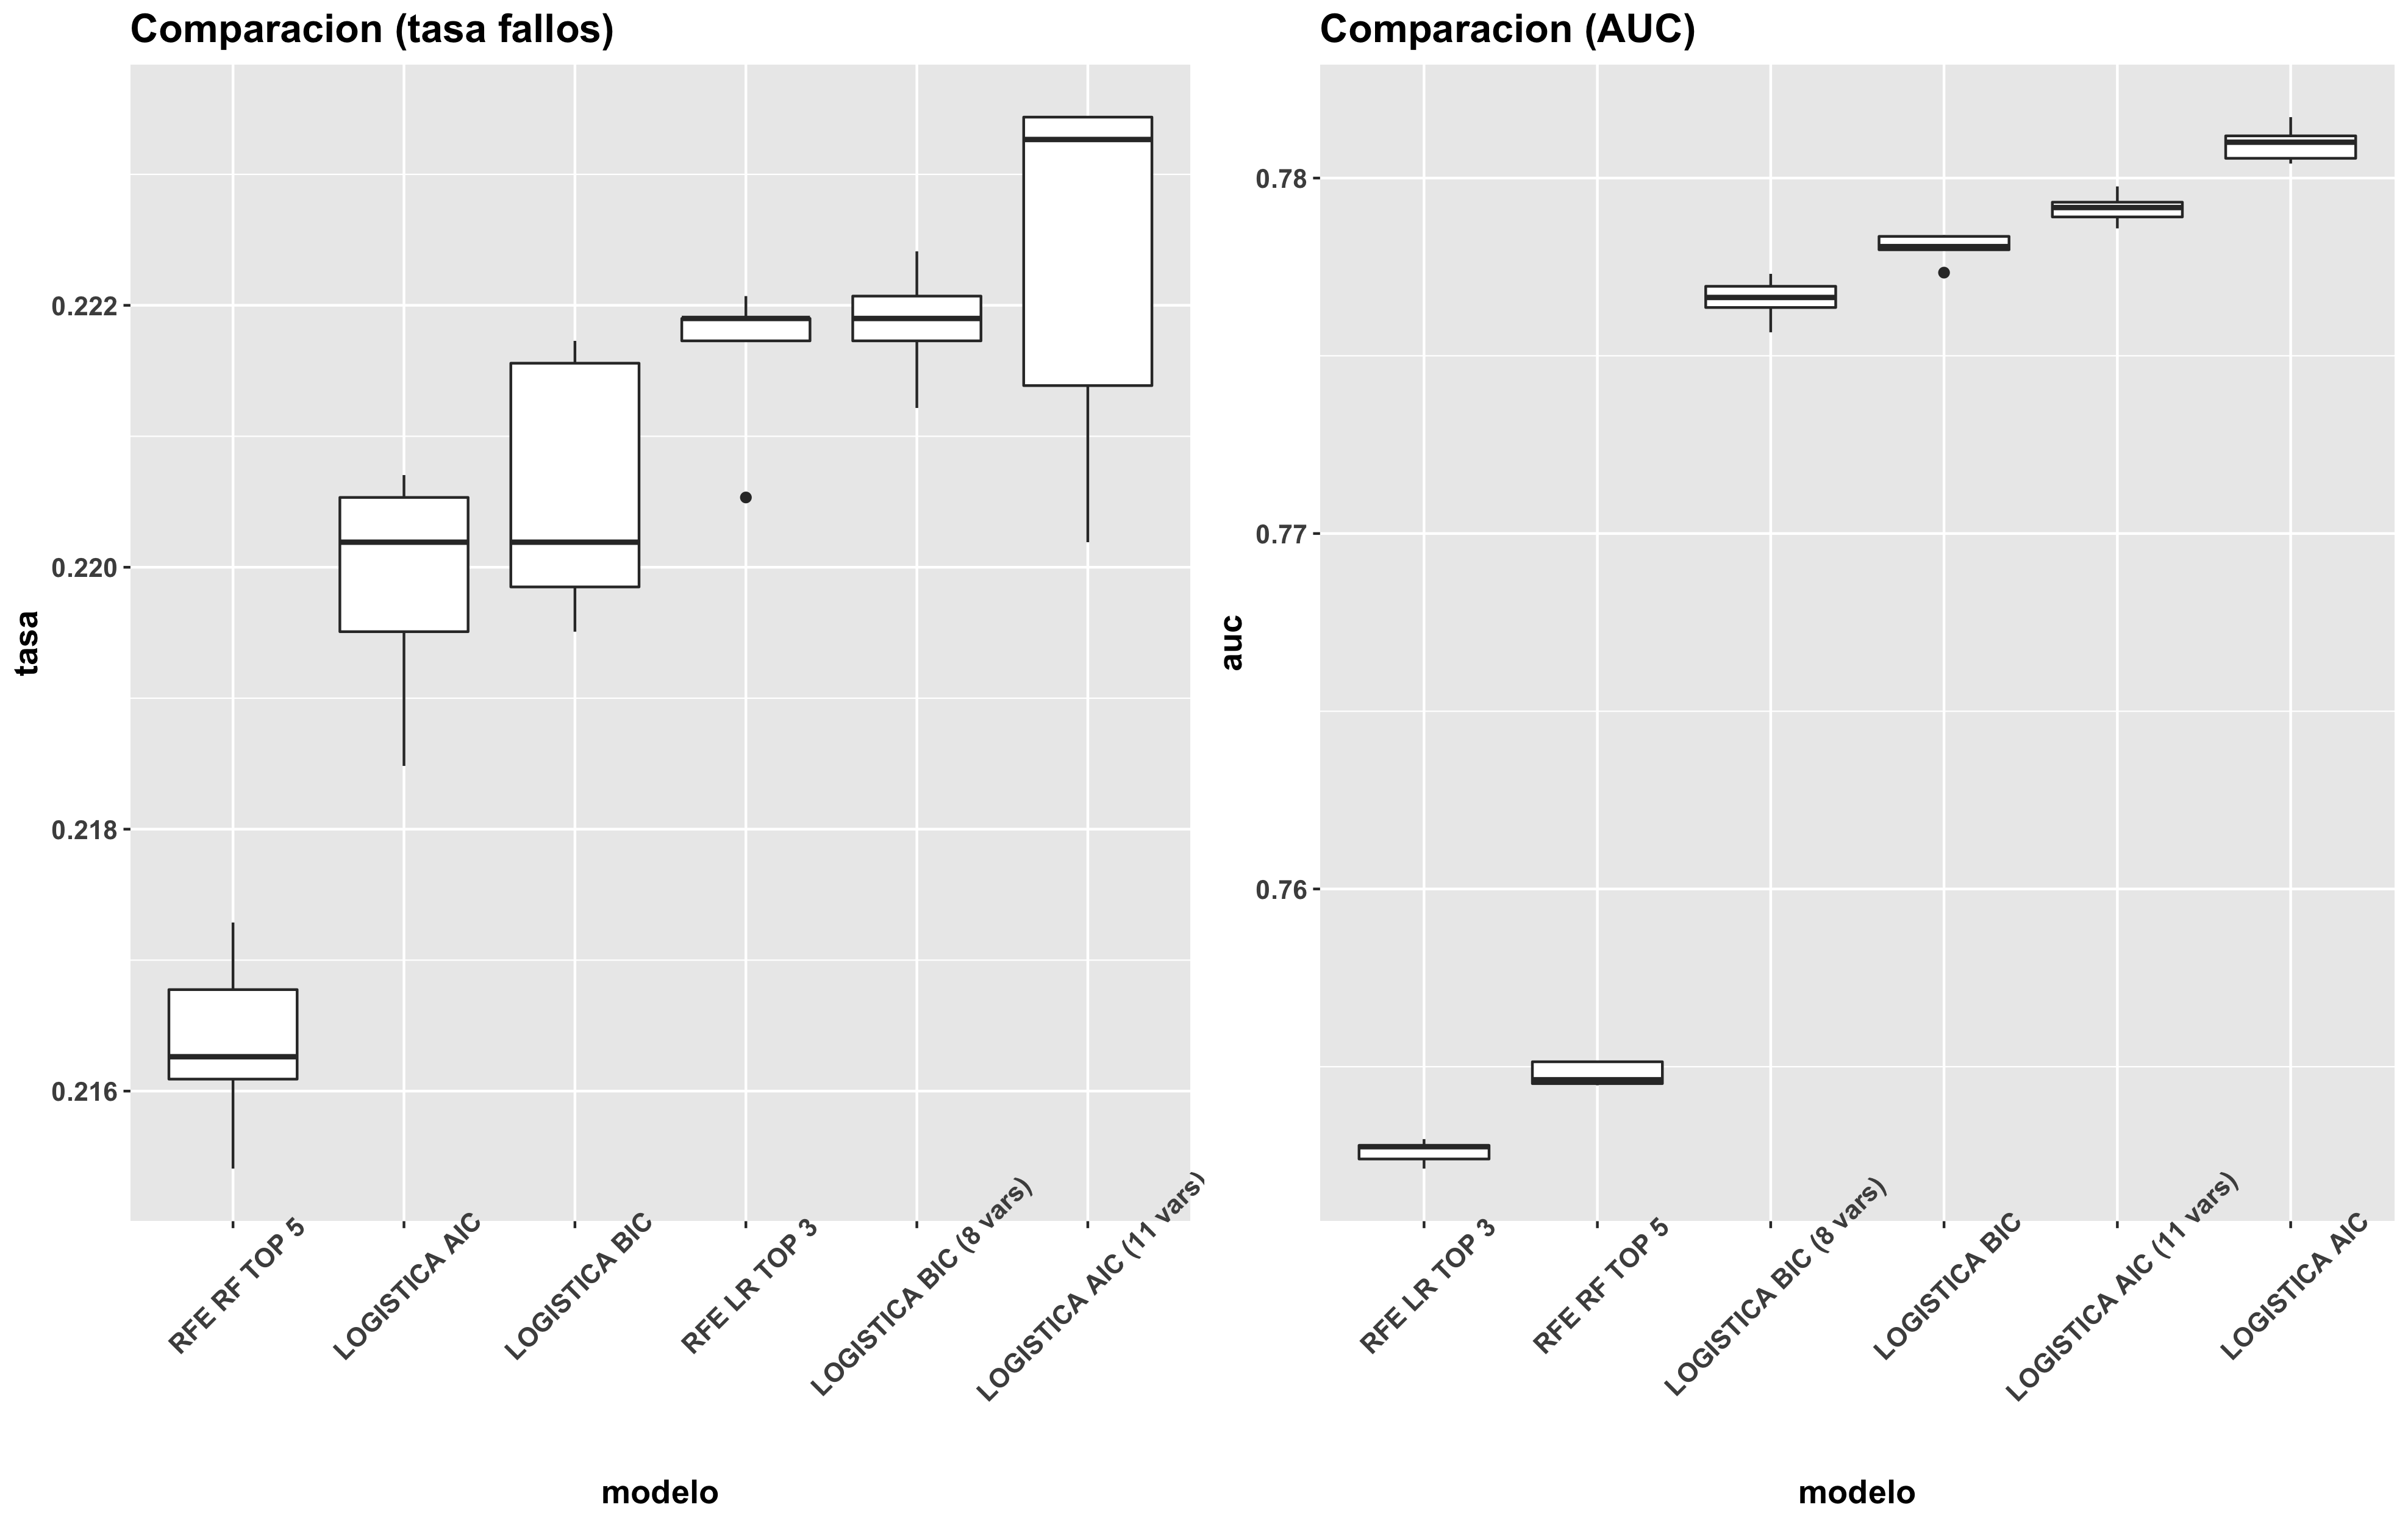
\includegraphics[width=0.97\linewidth,height=0.97\textheight,]{./charts/01_feature_selection_segunda_comparacion} 

}

\caption{Comparacion bajo logística (II)}\label{fig:unnamed-chunk-39}
\end{figure}

Incluso reduciendo el número de variables en ambos casos, aunque la tasa
de fallos aumente o el valor auc disiminuya ligeramente, la diferencia
no es muy significativa.

No obstante, uno de los aspectos que más ha llamada la atención ha sido
la selección de variables RFE con Random Forest, donde con tan solo 5
variables la accuracy aumentaba hasta cerca del 90 \%, mucho más alto
que un modelo logístico. Por tanto, ¿Y si entrenamos un pequeño modelo
random forest para observar la importancia de las variables tanto en
\emph{stepwise AIC} como en \emph{BIC}?

\begin{Shaded}
\begin{Highlighting}[]
\CommentTok{\#{-}{-} mtry (sqrt(numero de variables), por defecto)}
\NormalTok{rf\_modelo\_bic <{-}}\StringTok{ }\KeywordTok{train\_rf\_model}\NormalTok{(surgical\_dataset, formula.candidato.bic}\FloatTok{.2}\NormalTok{, }\DataTypeTok{ntree =} \DecValTok{1000}\NormalTok{, }
                                \DataTypeTok{grupos =} \DecValTok{5}\NormalTok{, }\DataTypeTok{repe =} \DecValTok{5}\NormalTok{, }\DataTypeTok{nodesize =} \DecValTok{10}\NormalTok{, }\DataTypeTok{seed =} \DecValTok{1234}\NormalTok{)}
\end{Highlighting}
\end{Shaded}

\begin{figure}[h!]

{\centering 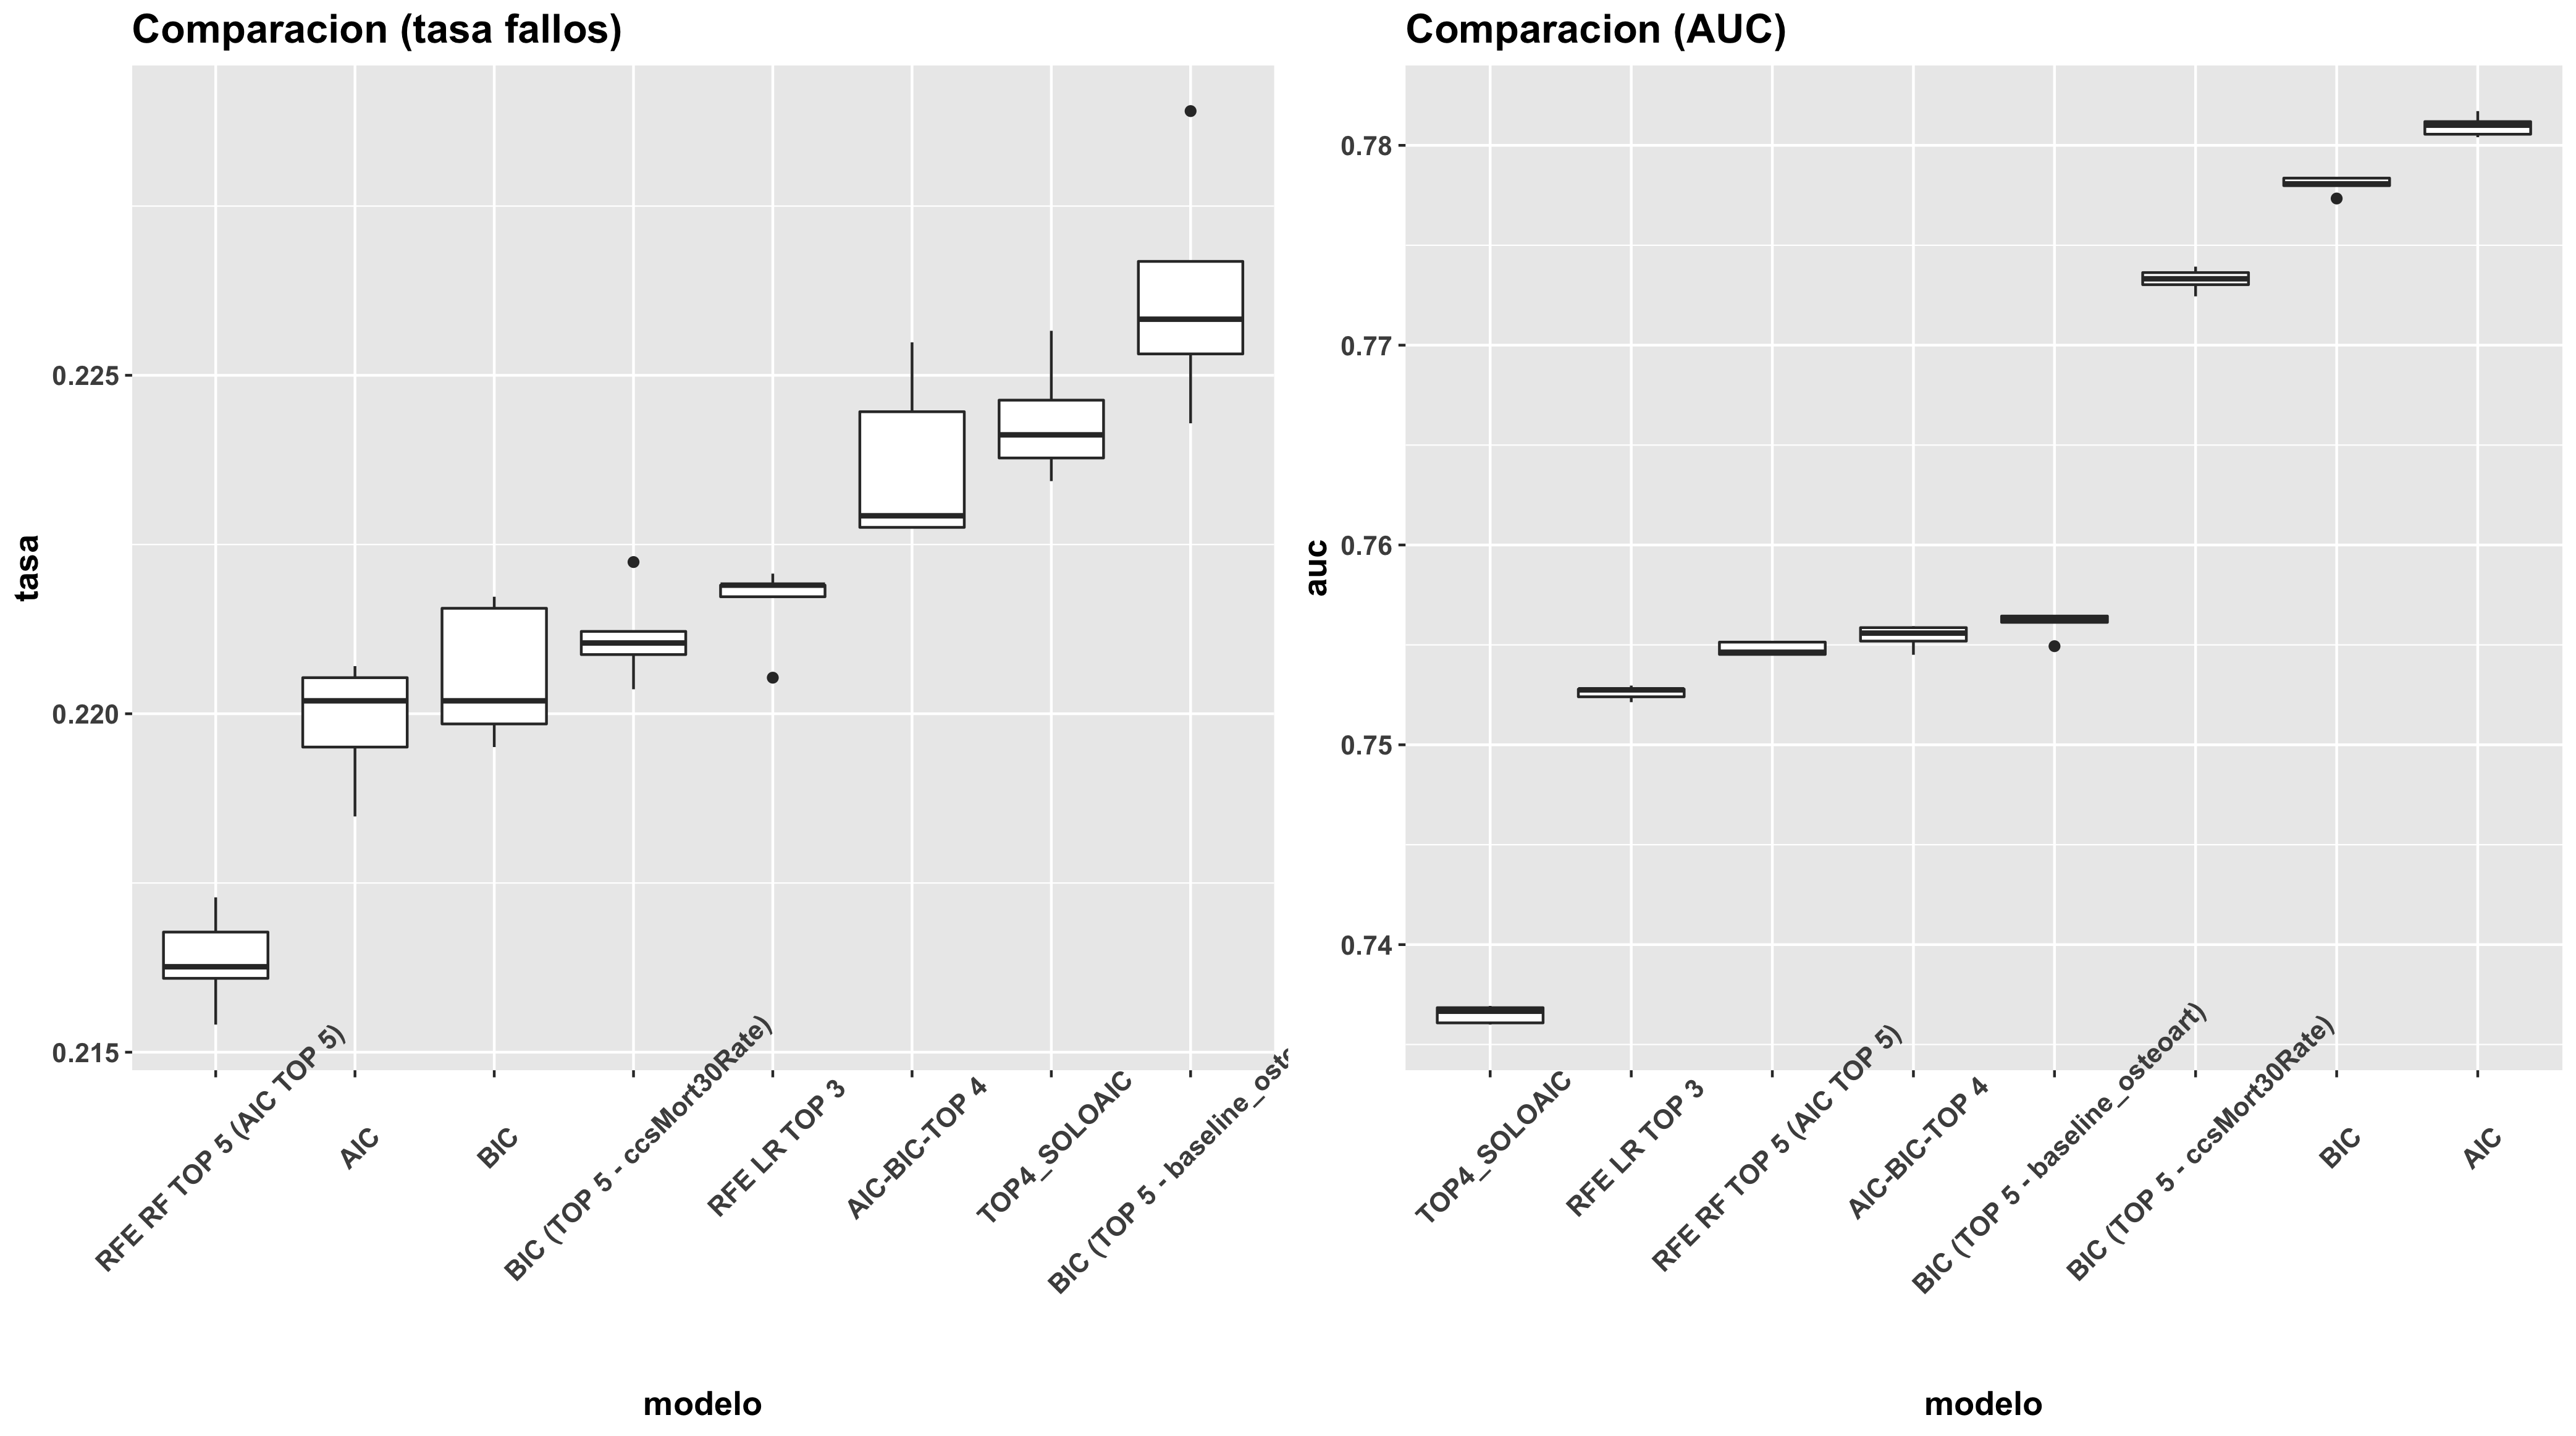
\includegraphics[width=0.99\linewidth,height=0.99\textheight,]{./charts/01_feature_selection_comparacion_random_forest} 

}

\caption{Importancia variables Random Forest (AIC y BIC)}\label{fig:unnamed-chunk-41}
\end{figure}

Analizando el gráfico de importancia, caben destacar cuatro principales
variables, \textbf{las cuales coinciden en ambos modelos, tanto en
\emph{stepwise AIC} como \emph{BIC}}: \emph{Age}, \emph{mortality\_rsi},
\emph{bmi} y \emph{ccsMort30Rate}. Por otro lado, en el modelo
\emph{AIC} cabe destacar, además, la variable \emph{ahrq\_ccs}. En
relación con el modelo \emph{BIC}, el contraste entre las cuatro
primeras variables y el resto de \emph{features} es más significativo,
de las cuales caben destacar \emph{baseline\_osteoart} y \emph{month.8},
con un nivel de importancia similar en el \emph{Random Forest}.

Por tanto, vista la importancia que presentan las variables en el modelo
\emph{Random Forest}, cabría preguntarse si realmente es necesario un
modelo con 11 u 8 variables, como es el caso de \emph{stepwise AIC} o
\emph{BIC}, respectivamente. Es decir, ¿Y si reducimos el modelo a las
4-5 variables más relevantes? Por ejemplo, una última comparación bajo
logística consistiría en (y en base al gráfico de importancia anterior)
analizar un modelo con las cuatro variables más importantes:

\begin{enumerate}
\def\labelenumi{\arabic{enumi}.}
\tightlist
\item
  \emph{Age}, \emph{mortality\_rsi}, \emph{bmi} y \emph{ccsMort30Rate}.
\end{enumerate}

Otro modelo logístico con las cinco variables más relevantes del
\emph{set} de variables \emph{BIC}:

\begin{enumerate}
\def\labelenumi{\arabic{enumi}.}
\setcounter{enumi}{1}
\tightlist
\item
  \emph{Age}, \emph{mortality\_rsi}, \emph{bmi}, \emph{ccsMort30Rate} y
  \emph{ahrq\_css} (coincide con con el modelo obtenido en \emph{RFE}
  con \emph{Random Forest}, por lo que lo denotamos como \emph{RFE RF
  TOP 5 (AIC TOP 5)}).
\end{enumerate}

Además de otros dos modelos con las cinco variables más relevantes en el
\emph{set} de variables \emph{AIC} (dado que \emph{baseline\_osteoart} y
\emph{month.8} son muy similares en cuanto a importancia se refiere,
realizamos la prueba con ambos \emph{sets}):

\begin{enumerate}
\def\labelenumi{\arabic{enumi}.}
\setcounter{enumi}{2}
\tightlist
\item
  \emph{Age}, \emph{mortality\_rsi}, \emph{bmi}, \emph{ccsMort30Rate} y
  \emph{baseline\_osteoart}.
\item
  \emph{Age}, \emph{mortality\_rsi}, \emph{bmi}, \emph{ccsMort30Rate} y
  \emph{month.8}.
\end{enumerate}

\begin{figure}[h!]

{\centering 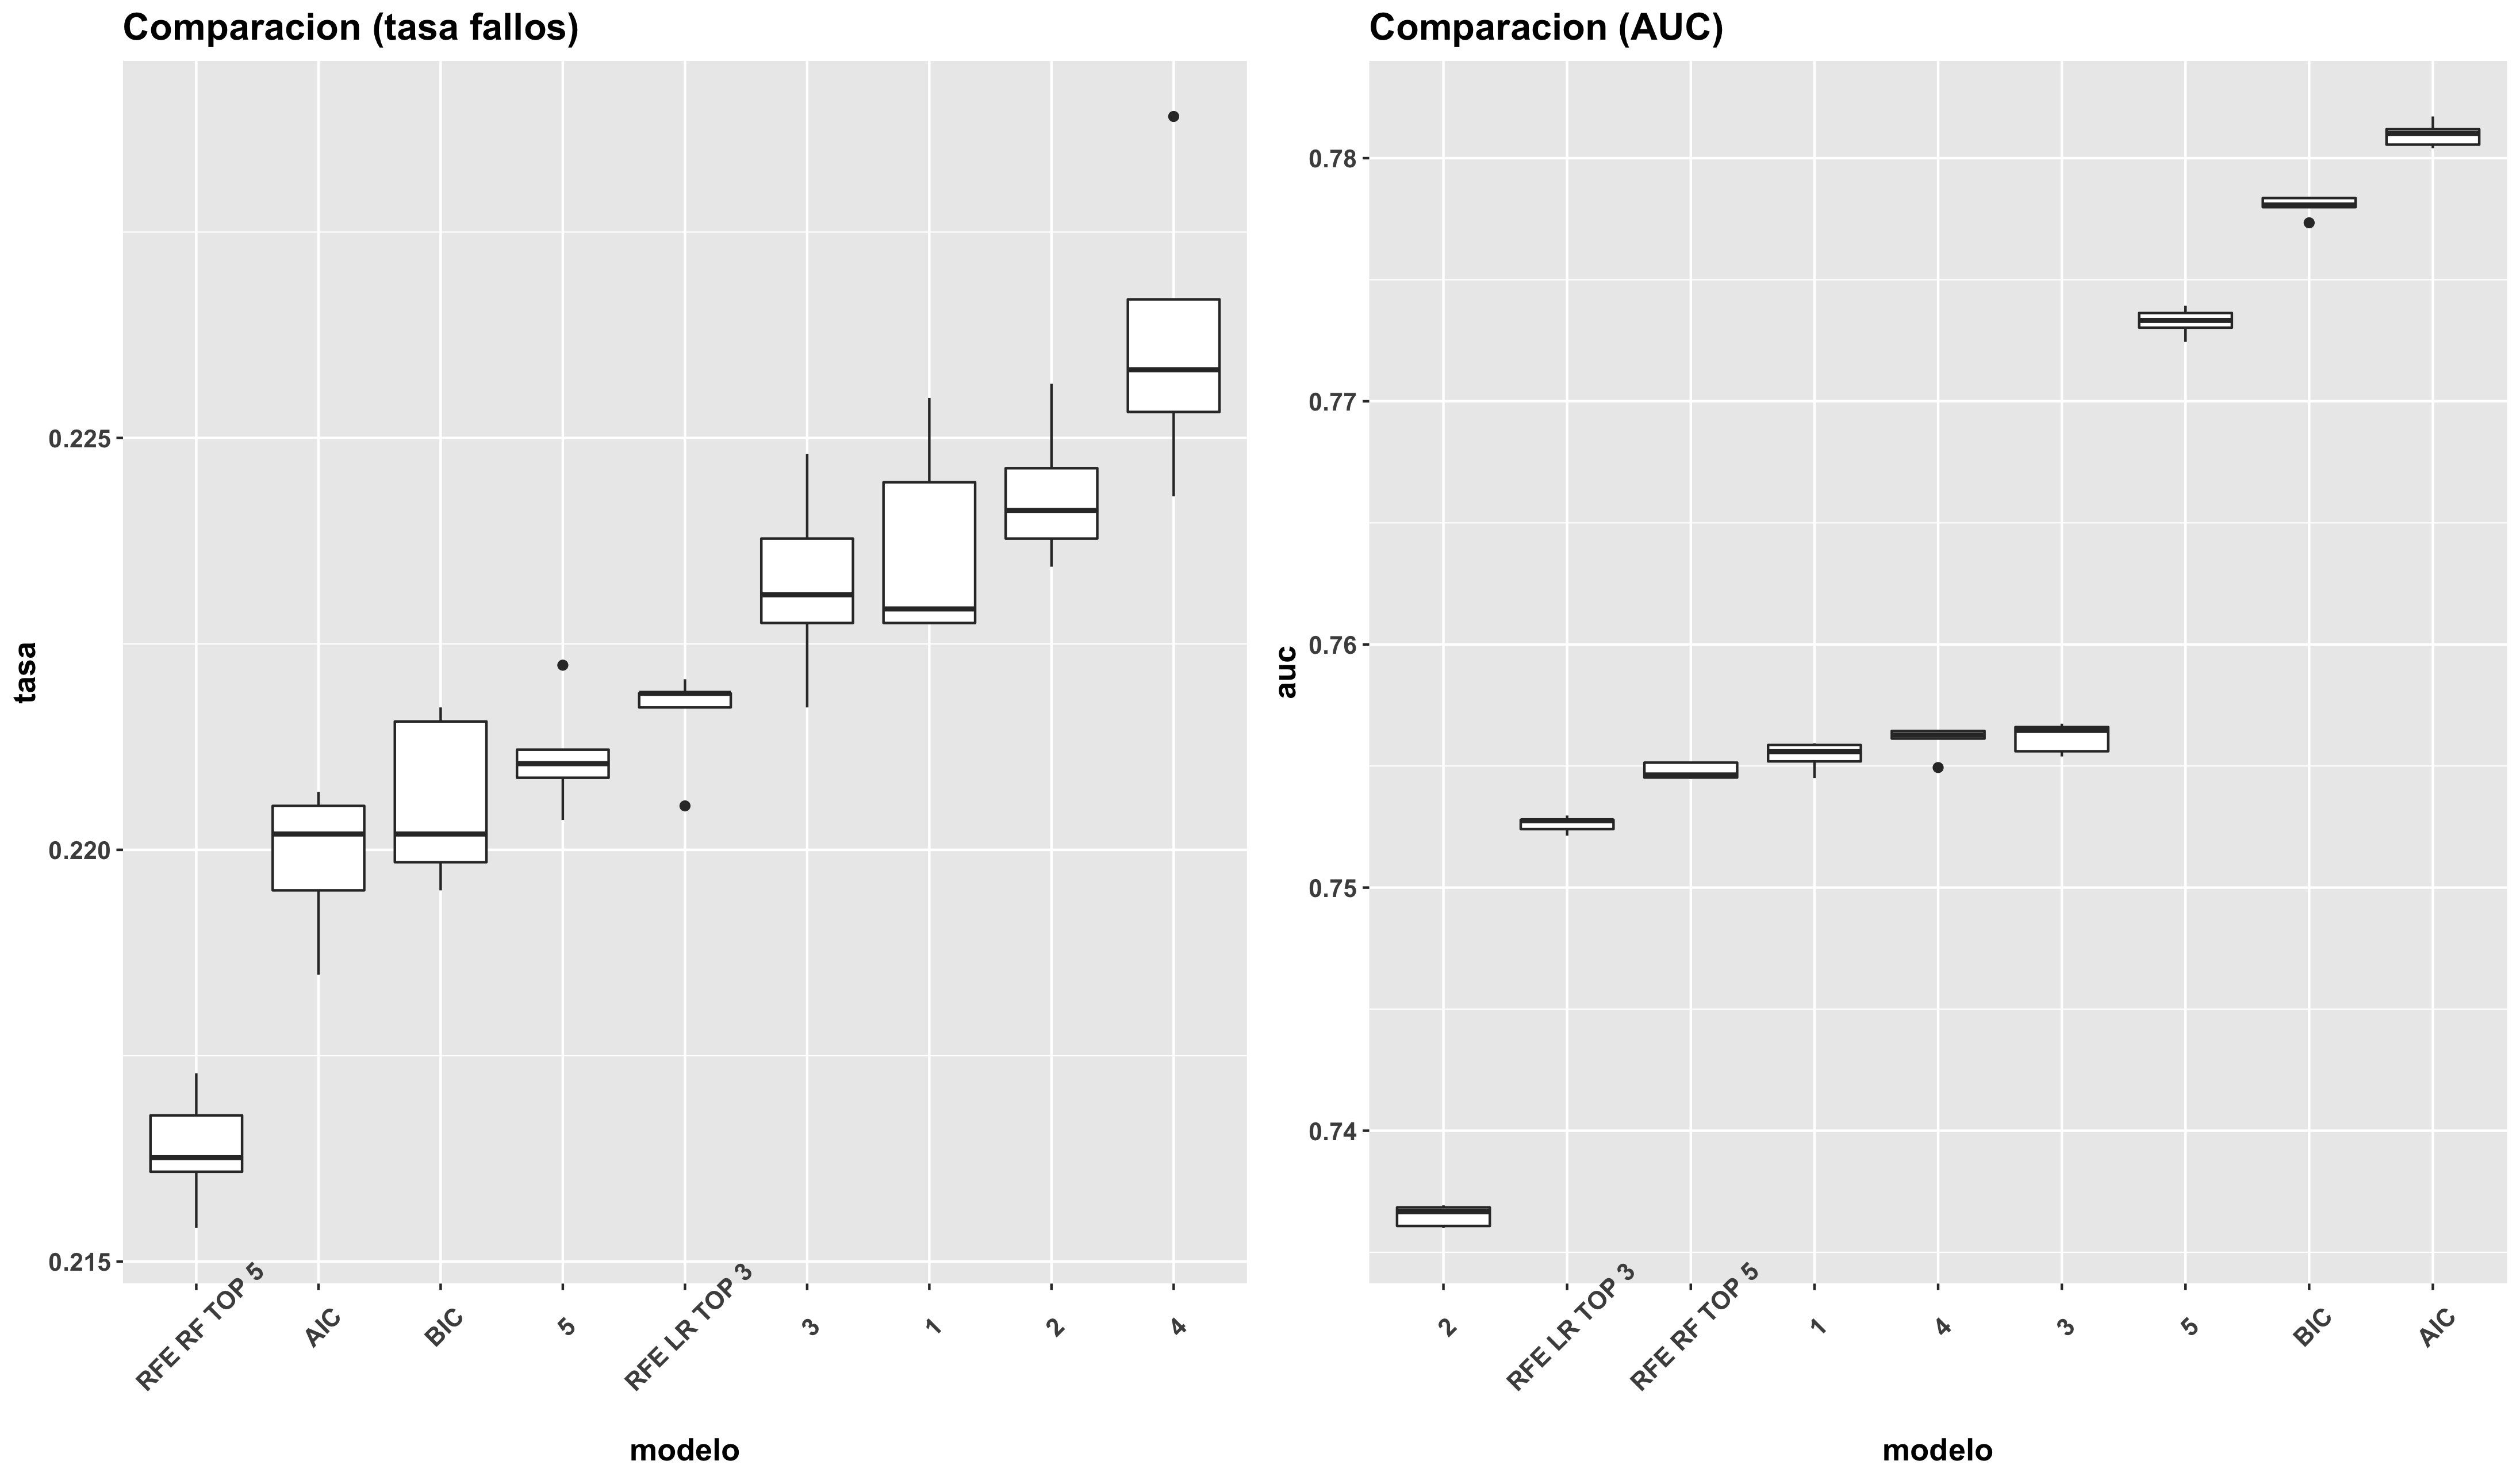
\includegraphics[width=0.99\linewidth,height=0.99\textheight,]{./charts/01_feature_selection_comparacion_final} 

}

\caption{Comparacion bajo logística (III)}\label{fig:unnamed-chunk-42}
\end{figure}

Como podemos comprobar, aunque la tasa de fallos sea similar tanto con
\emph{basline\_osteoart} como con \emph{month.8}, el valor AUC es
ligeramente superior, incluso cercano a los valores obtenidos por la
selección \emph{AIC}, \emph{BIC} original. Por otro lado, con tan solo
cuatro variables, aunque el valor AUC sea ligeramente inferior con
respecto al resto de \emph{sets}, la diferencia no es tan significativa
(0.755 a 0.775, aproximadamente).

Por tanto, de cara al resto de modelos \textbf{emplamos dos modelos
candidatos}:

\begin{verbatim}
##   n       modelo1       modelo2
## 1 1           Age           Age
## 2 2 mortality_rsi mortality_rsi
## 3 3           bmi           bmi
## 4 4 ccsMort30Rate ccsMort30Rate
## 5 5       month.8             -
\end{verbatim}

\begin{Shaded}
\begin{Highlighting}[]
\CommentTok{\#{-}{-}{-} Variables de los modelos candidatos}
\CommentTok{\#{-}{-}  Modelo 1}
\NormalTok{var\_modelo1 <{-}}\StringTok{ }\KeywordTok{c}\NormalTok{(}\StringTok{"mortality\_rsi"}\NormalTok{, }\StringTok{"ccsMort30Rate"}\NormalTok{, }\StringTok{"bmi"}\NormalTok{, }\StringTok{"month.8"}\NormalTok{, }\StringTok{"Age"}\NormalTok{)}

\CommentTok{\#{-}{-} Modelo 2}
\NormalTok{var\_modelo2 <{-}}\StringTok{ }\KeywordTok{c}\NormalTok{(}\StringTok{"mortality\_rsi"}\NormalTok{, }\StringTok{"bmi"}\NormalTok{, }\StringTok{"month.8"}\NormalTok{, }\StringTok{"Age"}\NormalTok{)}
\end{Highlighting}
\end{Shaded}

\hypertarget{tuneo-y-comparaciuxf3n-final}{%
\subsection{4.7 Tuneo y comparación
final}\label{tuneo-y-comparaciuxf3n-final}}

Finalmente, realizamos una última comparación de ambos modelos
candidatos, \textbf{aumentando la validación cruzada de 5 a 10
repeticiones}:

\begin{figure}[h!]

{\centering 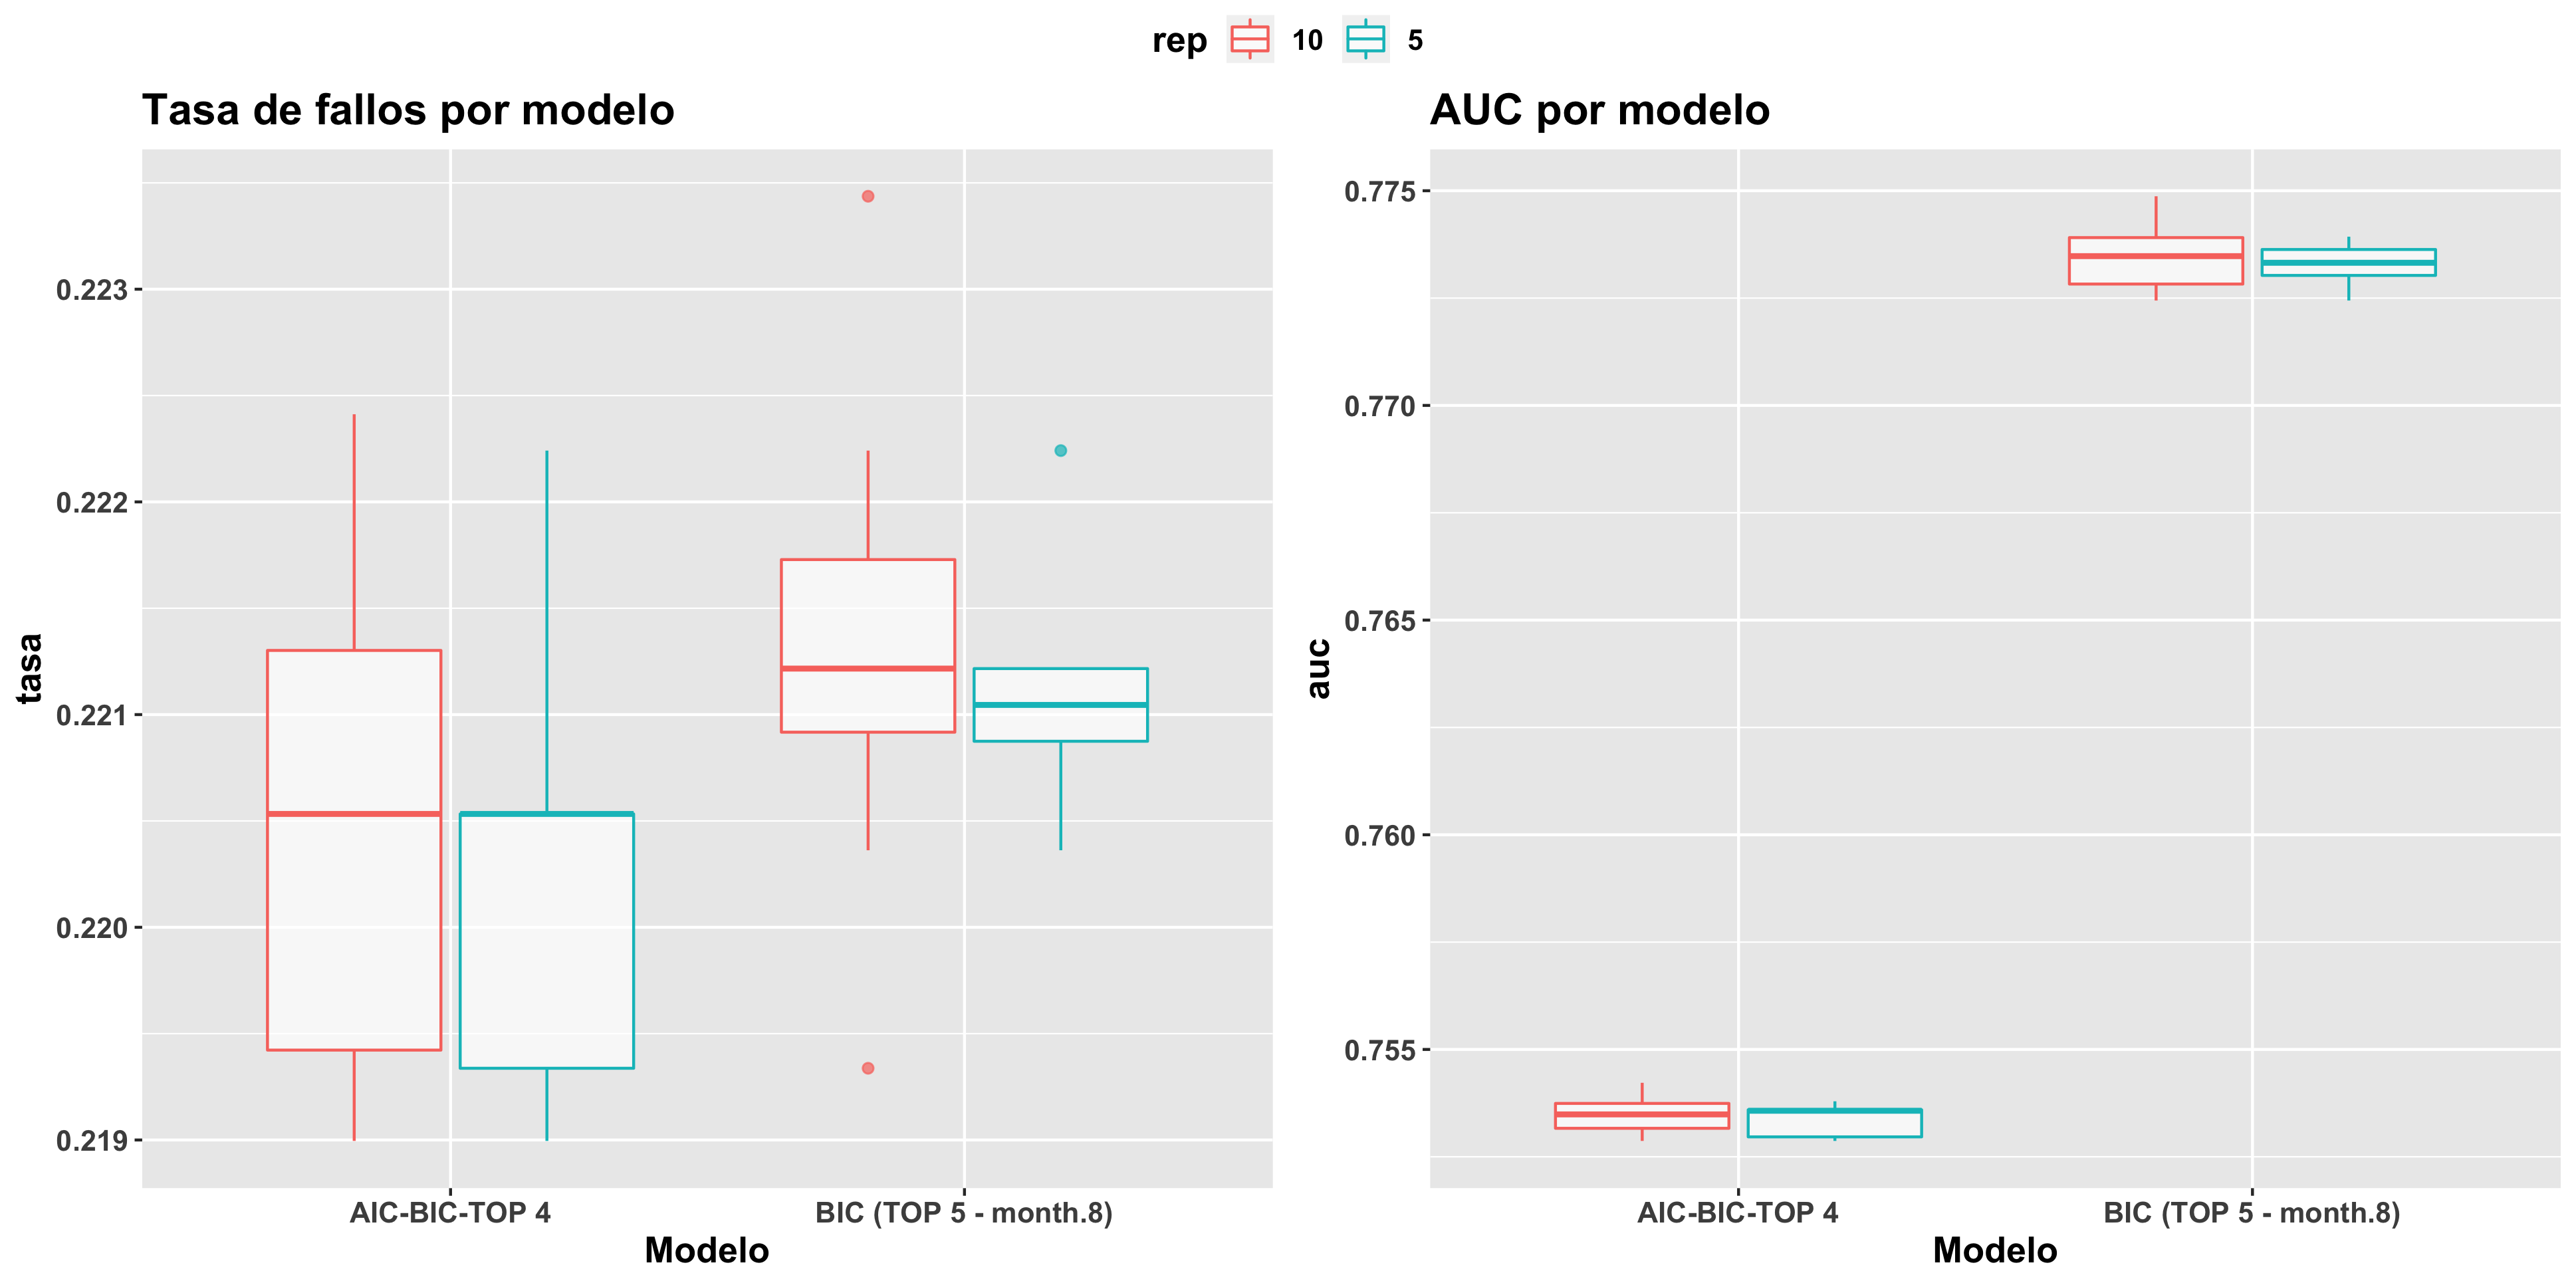
\includegraphics[width=0.99\linewidth,height=0.99\textheight,]{./charts/01_feature_selection_comparacion_5_10_rep} 

}

\caption{Comparacion final logística (5-10 rep.)}\label{fig:unnamed-chunk-45}
\end{figure}

A primera vista, al aumentar el número de repeticiones, la varianza en
ambos modelos es muy similar, con una ventaja en el segundo modelo en
cuanto a AUC se refiere (0.775 frente a 0.755, aproximadamente). Por
otro lado, si nos fijamos en las estadísticas obtenidas a partir de los
datos \emph{test}:

\begin{verbatim}
##                 modelo precision sensibilidad especificidad valor_pred_pos
## 1 Modelo 1 (BIC TOP 5)    0.7940      0.67730       0.81011        0.33013
## 2     Modelo 2 (top 4)    0.7824      0.66707       0.79434        0.25194
##   valor_pred_neg
## 1        0.94783
## 2        0.95830
\end{verbatim}

Observamos que la sensibilidad de ambos modelos ronda el 66-67 \%,
mientras que la especificidad aumenta hasta el 80 \%, aproximadamente.
Es decir, con un modelo lineal como es el caso de la regresión logística
conseguimos clasificar la mayoría de los pacientes a 0 (sin
complicaciones). Sin embargo, tanto el valor predictivo positivo como la
sensibilidad nos indican justo con lo contrario en relación a los
pacientes con complicaciones:

\begin{enumerate}
\def\labelenumi{\arabic{enumi}.}
\item
  \textbf{Valor predictivo positivo} (en torno al 25-33 \% en ambos
  modelos), lo que se traduce en un alto número de falsos positivos.
\item
  \textbf{Sensbilidad} (en torno al 66-67 \% en ambos modelos), lo que
  se traduce en un alto número de falsos negativos.
\end{enumerate}

\hypertarget{modelos-iniciales-con-h2o}{%
\section{5. Modelos iniciales con H2O}\label{modelos-iniciales-con-h2o}}

Una realizada la selección de variables y decantarnos por dos posibles
\emph{sets} de variables, antes de comenzar con el tuneo de
hiperparámetros, \textbf{realizamos un modelo \emph{autoML} por cada
\emph{set} de variables}. De este modo, podremos comprobar, de forma
orientativa:

\begin{enumerate}
\def\labelenumi{\arabic{enumi}.}
\tightlist
\item
  Qué modelo o modelos son los más adecuados, tanto a nivel AUC como en
  tasa de fallos.
\item
  Del mejor o mejores modelos, qué parámetros se ha empleado.
\end{enumerate}

\hypertarget{modelo-1-bic-top-5}{%
\subsection{5.1 Modelo 1 (BIC TOP 5)}\label{modelo-1-bic-top-5}}

\begin{Shaded}
\begin{Highlighting}[]
\CommentTok{\#   Modelo 1}
\NormalTok{aml\_}\DecValTok{1}\NormalTok{ <{-}}\StringTok{ }\KeywordTok{h2o.automl}\NormalTok{(}\DataTypeTok{x =}\NormalTok{ var\_modelo1, }\DataTypeTok{y =}\NormalTok{ target, }
                    \DataTypeTok{training\_frame =}\NormalTok{ surgical\_dataset\_h, }\DataTypeTok{nfolds =} \DecValTok{5}\NormalTok{, }\DataTypeTok{seed =} \DecValTok{1234}\NormalTok{,}
                    \DataTypeTok{balance\_classes =} \OtherTok{TRUE}\NormalTok{, }\DataTypeTok{keep\_cross\_validation\_predictions =} \OtherTok{TRUE}\NormalTok{,}
                    \DataTypeTok{max\_models =} \DecValTok{10}\NormalTok{)}
\end{Highlighting}
\end{Shaded}

\begin{verbatim}
                                              model_id       auc   logloss mean_per_class_error
1                         GBM_5_AutoML_20210422_174850 0.9211350 0.2591059            0.1608837
2  StackedEnsemble_BestOfFamily_AutoML_20210422_174850 0.9208431 0.2647496            0.1603029
3                         GBM_1_AutoML_20210422_174850 0.9200581 0.2690935            0.1659645
4     StackedEnsemble_AllModels_AutoML_20210422_174850 0.9200033 0.2647962            0.1676764
5                         GBM_2_AutoML_20210422_174850 0.9190857 0.2695043            0.1648937
6                     XGBoost_3_AutoML_20210422_174850 0.9189663 0.2613378            0.1651901
7       XGBoost_grid__1_AutoML_20210422_174850_model_1 0.9189402 0.2629065            0.1675371
8           GBM_grid__1_AutoML_20210422_174850_model_1 0.9187735 0.2763313            0.1689585
9                         GBM_3_AutoML_20210422_174850 0.9175951 0.2725404            0.1757392
10                    XGBoost_2_AutoML_20210422_174850 0.9169047 0.2717032            0.1707306
\end{verbatim}

En un primer análisis, de todos los modelos \emph{autoML} creados,
\textbf{los modelos \emph{gradient boosting}, \emph{ensemble} y
\emph{xgboost} obtienen los mejores resultados}, con un AUC en torno a
0.92, así como un error medio por cada clase de 0.16-0.17,
aproximadamente. Por otro lado, si analizamos los parámetros del mejor
modelo, concretamente \emph{gradient boosting}:

\begin{verbatim}
##                 modelo ntrees max_depth sample_rate col_sample_rate
## 1 Modelo 1 (BIC TOP 5)     82        15         0.8             0.8
##   col_sample_rate_per_tree
## 1                      0.8
\end{verbatim}

Analizando los parámetros, por lo general \emph{h2o} \textbf{opta por un
modelo \emph{gbm} sencillo, con un número bajo de árboles (inferior a
100), un profundidad moderada en cada árbol (15), además de sortear no
solo observaciones, sino además variables (en torno al 80 \%)}.

\hypertarget{modelo-2-aic-bic-top-4}{%
\subsection{5.2 Modelo 2 (AIC-BIC top 4)}\label{modelo-2-aic-bic-top-4}}

\begin{verbatim}
                                              model_id       auc   logloss  mean_per_class_error
1                         GBM_5_AutoML_20210422_182719 0.9096419 0.2700148            0.1646700
2  StackedEnsemble_BestOfFamily_AutoML_20210422_182719 0.9088350 0.2712222            0.1666722
3     StackedEnsemble_AllModels_AutoML_20210422_182719 0.9083655 0.2708531            0.1683963
4                     XGBoost_3_AutoML_20210422_182719 0.9083145 0.2683037            0.1735557
5                         GBM_1_AutoML_20210422_182719 0.9075638 0.2769396            0.1730899
6                         GBM_2_AutoML_20210422_182719 0.9072236 0.2767946            0.1770094
7       XGBoost_grid__1_AutoML_20210422_182719_model_1 0.9065834 0.2696259            0.1678335
8                     XGBoost_2_AutoML_20210422_182719 0.9064648 0.2756899            0.1671682
9                     XGBoost_1_AutoML_20210422_182719 0.9047755 0.2746863            0.1725274
10          GBM_grid__1_AutoML_20210422_182719_model_1 0.9044822 0.3115999            0.1720491
\end{verbatim}

Nuevamente, con el segundo \emph{set} de variables continua optando por
un modelo \emph{grandient boosting}, con un AUC muy similar al primer
\emph{set} de variables (0.90 frente a 0.92). Además, si analizamos los
parámetros del mejor modelo:

\begin{verbatim}
##                    modelo ntrees max_depth sample_rate col_sample_rate
## 1    Modelo 1 (BIC TOP 5)     82        15         0.8             0.8
## 2 Modelo 2 (AIC-BIC-top4)     72        15         0.8             0.8
##   col_sample_rate_per_tree
## 1                      0.8
## 2                      0.8
\end{verbatim}

Salvo el número de árboles, el resto de parámetros coinciden. Por tanto,
de cara a la elaboración de los modelos, \textbf{comprobaremos si el
mejor modelo en ambos \emph{sets} es, efectivamente, un modelo
\emph{gbm}, o si al menos está entre los mejores}.

\hypertarget{redes-neuronales}{%
\section{6. Redes neuronales}\label{redes-neuronales}}

\hypertarget{modelo-1-bic-top-5-1}{%
\subsection{6.1 Modelo 1 (BIC TOP 5)}\label{modelo-1-bic-top-5-1}}

A continuación, procedemos con el tuneado del primer modelo
\emph{Machine Learning}: la red neuronal, comenzando con el primer
\emph{set} (5 variables input). En primera instancia, analicemos el
número de nodos necesario para obtener entre 20 y 30 observaciones por
parámetro, teniendo 5 variables \emph{input}:

\begin{enumerate}
\def\labelenumi{\arabic{enumi}.}
\item
  Con 20 observaciones por parámetro: \[
  h * (k + 1) + h + 1 = 5854 / 20 = 292 \text{ parámetros}
  \] \[
  \text{Con } k = 5 \text{ variables input, entonces: } 7 * h + 1 = 292. \text{ Es decir}, 41-42 \text{ nodos}
  \]
\item
  Con 30 observaciones por parámetro: \[
  h * (k + 1) + h + 1 = 5854 / 30 = 195 \text{ parámetros}
  \] \[
  \text{Con } k = 5 \text{ variables input, entonces: } 7 * h + 1 = 195 \text{. Es decir}, 27-28 \text{ nodos}
  \]
\end{enumerate}

En primera instancia, dado que dispone de tan solo cinco variables ,
probablemente no serán necesarios tantos nodos. No obstante, realizamos
un primer tuneo con varios tamaños (desde 5 hasta 40):

\begin{Shaded}
\begin{Highlighting}[]
\NormalTok{size.candidato}\FloatTok{.1}\NormalTok{ <{-}}\StringTok{ }\KeywordTok{c}\NormalTok{(}\DecValTok{5}\NormalTok{, }\DecValTok{10}\NormalTok{, }\DecValTok{15}\NormalTok{, }\DecValTok{20}\NormalTok{, }\DecValTok{25}\NormalTok{, }\DecValTok{30}\NormalTok{, }\DecValTok{35}\NormalTok{, }\DecValTok{40}\NormalTok{)}
\NormalTok{decay.candidato}\FloatTok{.1}\NormalTok{ <{-}}\StringTok{ }\KeywordTok{c}\NormalTok{(}\FloatTok{0.1}\NormalTok{, }\FloatTok{0.01}\NormalTok{, }\FloatTok{0.001}\NormalTok{)}

\NormalTok{cvnnet.candidato}\FloatTok{.1}\NormalTok{ <{-}}\StringTok{ }\KeywordTok{cruzadaavnnetbin}\NormalTok{(}\DataTypeTok{data=}\NormalTok{surgical\_dataset,}\DataTypeTok{vardep=}\NormalTok{target,}
                                       \DataTypeTok{listconti=}\NormalTok{var\_modelo1, }\DataTypeTok{listclass=}\KeywordTok{c}\NormalTok{(}\StringTok{""}\NormalTok{),}
                                       \DataTypeTok{grupos=}\DecValTok{5}\NormalTok{,}\DataTypeTok{sinicio=}\DecValTok{1234}\NormalTok{,}\DataTypeTok{repe=}\DecValTok{5}\NormalTok{, }\DataTypeTok{size=}\NormalTok{size.candidato}\FloatTok{.1}\NormalTok{,}
                                       \DataTypeTok{decay=}\NormalTok{decay.candidato}\FloatTok{.1}\NormalTok{,}\DataTypeTok{repeticiones=}\DecValTok{5}\NormalTok{,}\DataTypeTok{itera=}\DecValTok{200}\NormalTok{)}
\end{Highlighting}
\end{Shaded}

\begin{verbatim}
##    id size decay  Accuracy
## 1   1   25 0.010 0.8950798
## 2   2   30 0.010 0.8947370
## 3   3   20 0.010 0.8945332
## 4   4   35 0.010 0.8939514
## 5   5   30 0.001 0.8934057
## 6   6   40 0.010 0.8921747
## 7   7   25 0.001 0.8919025
## 8   8   35 0.001 0.8914928
## 9   9   15 0.010 0.8905699
## 10 10   20 0.001 0.8899210
## 11 11   40 0.001 0.8892375
## 12 12   25 0.100 0.8862640
## 13 13   35 0.100 0.8855127
## 14 14   30 0.100 0.8847618
## 15 15   20 0.100 0.8841129
## 16 16   40 0.100 0.8837363
## 17 17   15 0.100 0.8829166
## 18 18   15 0.001 0.8794649
## 19 19   10 0.010 0.8793648
## 20 20   10 0.100 0.8653218
## 21 21   10 0.001 0.8557885
## 22 22    5 0.010 0.8237056
## 23 23    5 0.100 0.8129454
## 24 24    5 0.001 0.8113744
\end{verbatim}

Analizando la tabla anterior, empleando un \emph{decay} o
\emph{learning\_rate} de 0.01, \textbf{el modelo obtiene muy buenos
resultados, mejores incluso que la regresión logística, un indicativo de
la no linealidad de las variables}. Por otro lado, y en relación con el
número de nodos ¿Merece aumentar hasta 20, 30 o incluso 40 nodos? En
vista a los resultados, no lo parece. A modo de ejemplo, con tan solo 15
nodos y un \emph{decay} de 0.01, el valor de \emph{accuracy} alcanza un
89 \%, mientras que con 20, 30 o 40 nodos, la diferencia es de tan solo
unas milésimas (no estamos ganando lo suficiente como para decantarnos
por un modelo más complejo). Por tanto, una buena alternativa sería
emplear 15 nodos (10 tampoco sería una mala opción, aunque comienza a
decaer hasta el 87 \%).

No obstante, con un \emph{decay} de 0.01, analicemos tanto el sesgo como
la varianza en base al número de nodos:

\begin{figure}[h!]

{\centering 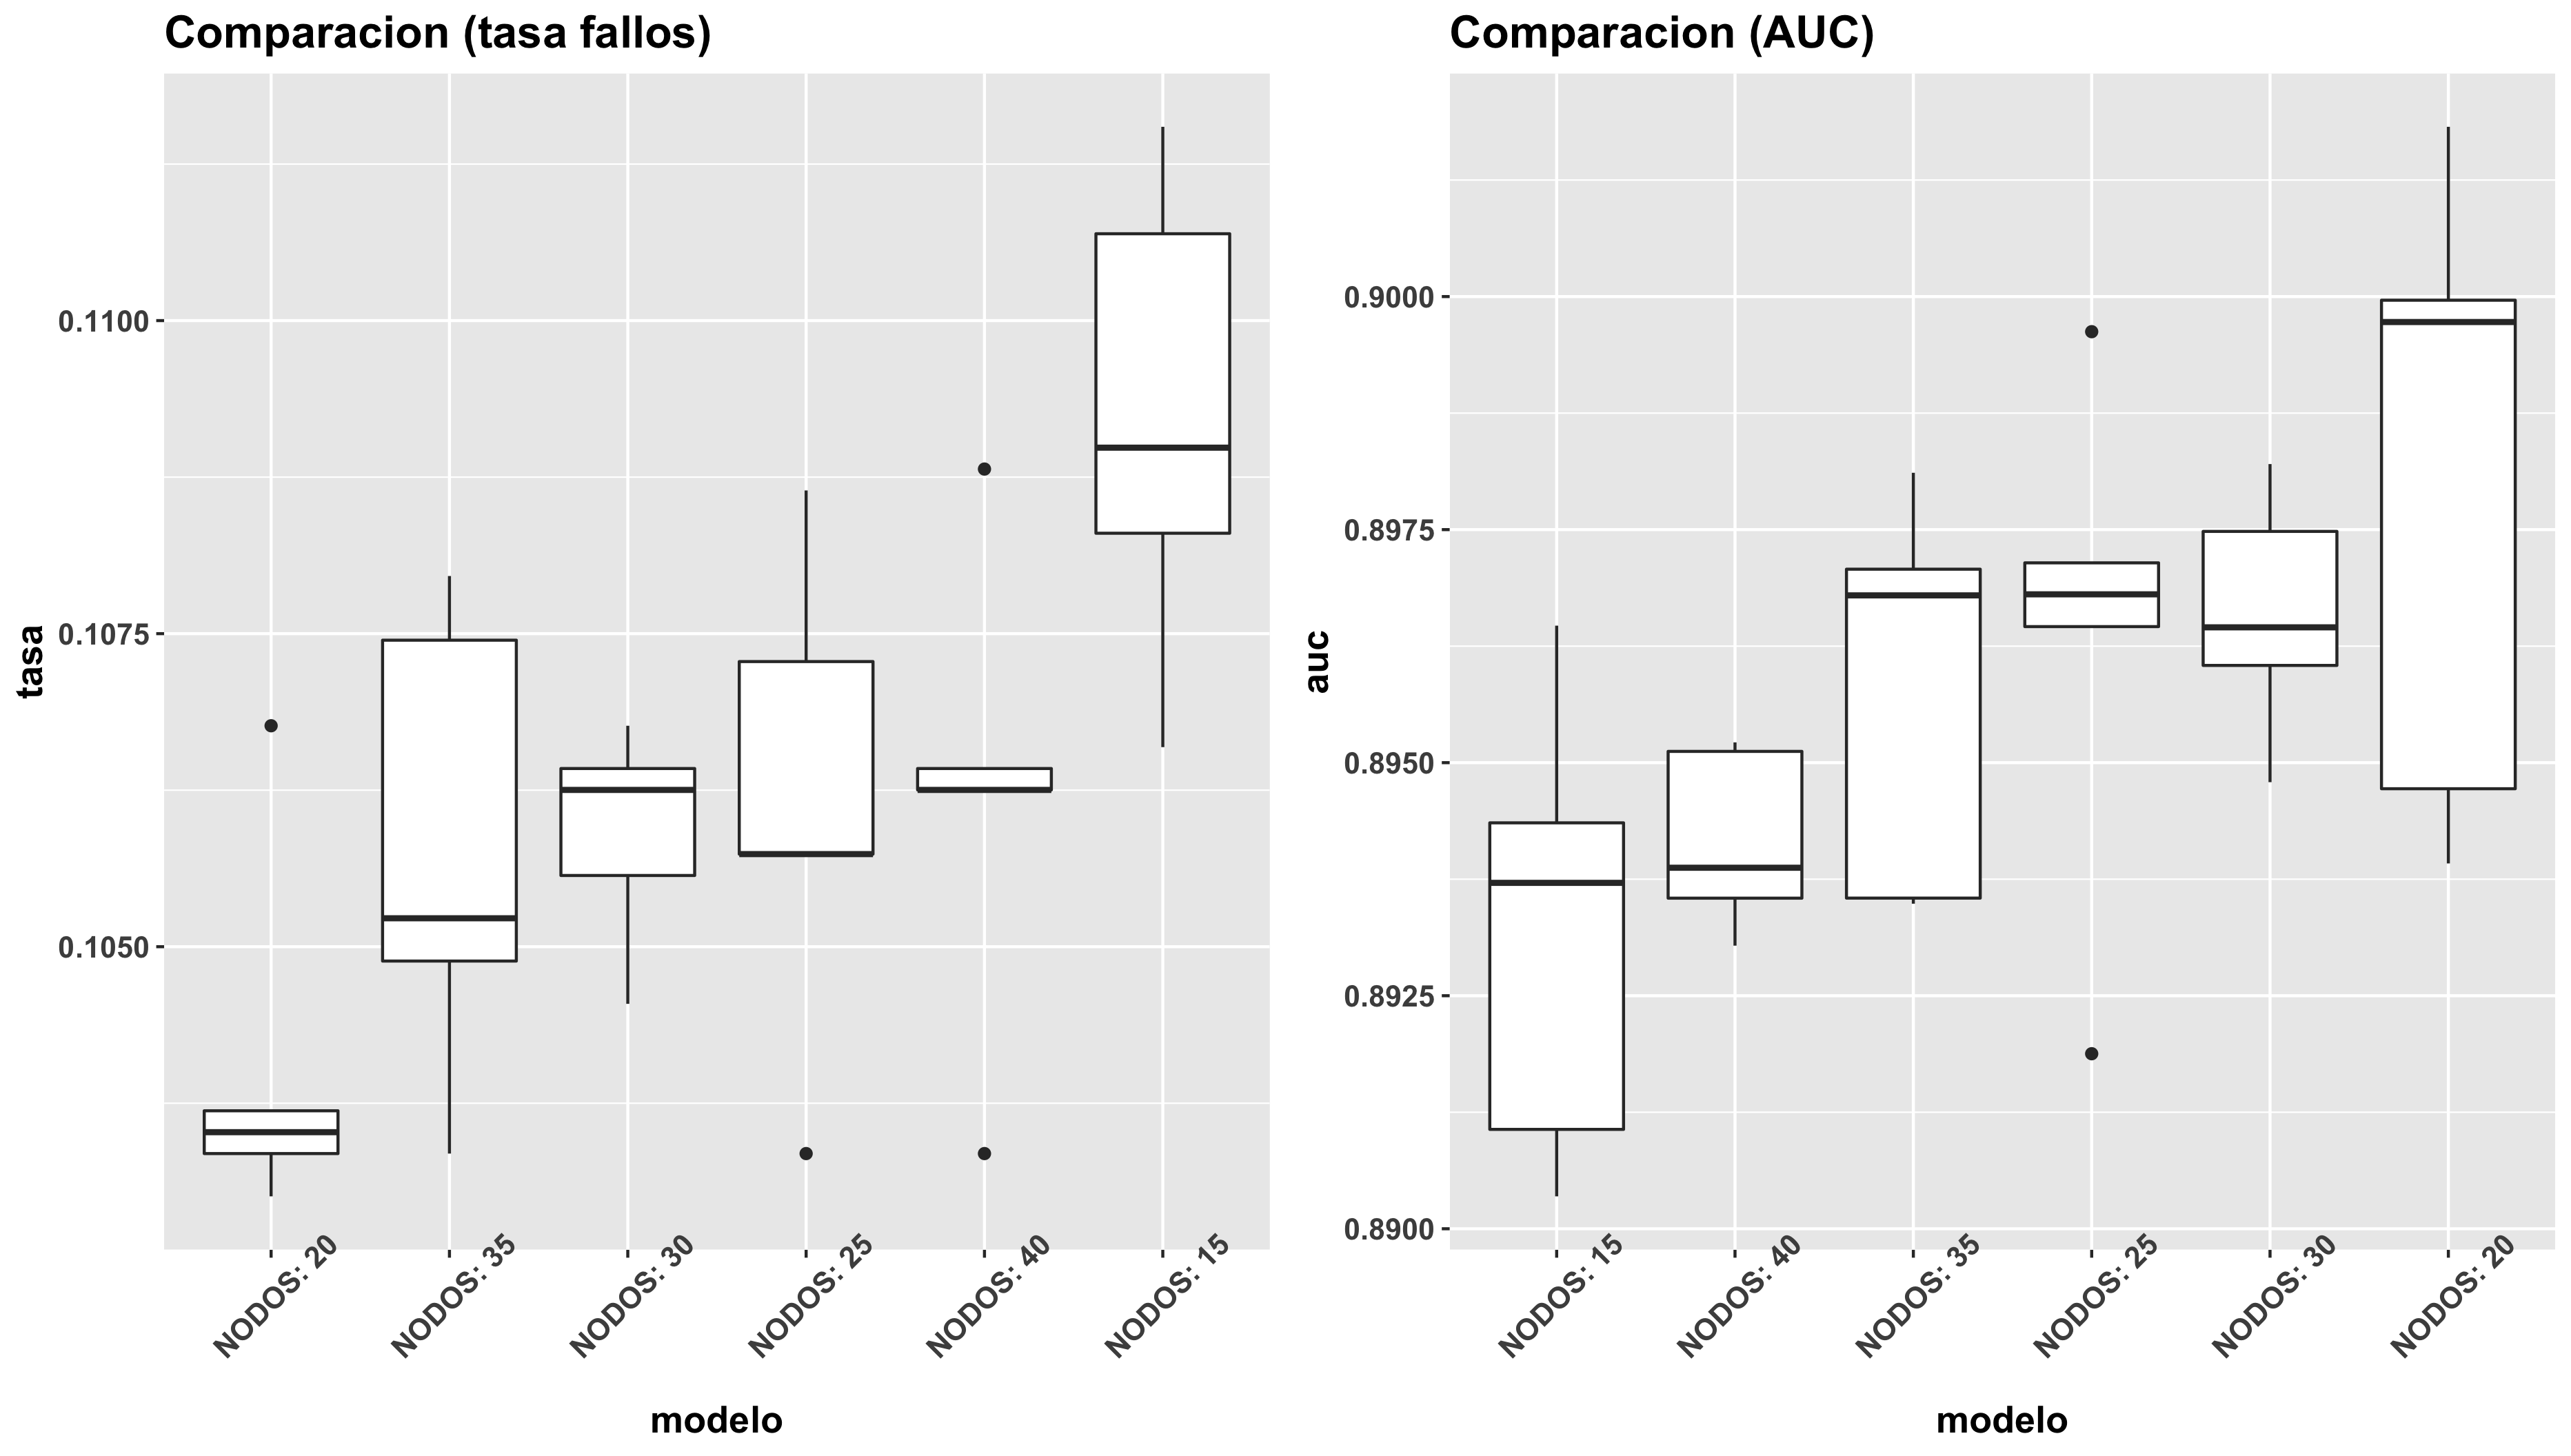
\includegraphics[width=0.99\linewidth,height=0.99\textheight,]{./charts/02_comparacion_tasa_auc_modelo1} 

}

\caption{Comparacion avnnet modelo 1}\label{fig:unnamed-chunk-52}
\end{figure}

Como primera impresión, y en base al mejor AUC, un modelo con 20, 25 o
30 nodos sería una buena alternativa, de no ser por un aspecto clave:
\textbf{la escala de los ejes}. En relación con la tasa de fallos, la
diferencia de error entre un modelo con 15 nodos y un modelo con 20 es
muy pequeña (de 0.11 a 0.105), además de que la varianza del modelo con
15 nodos (elevada desde un punto de vista gráfico), la escala del eje
puede llevar a engaño, dado que sus valores de error oscilan entre
0.1075 y 0.11. Por otro lado, la diferencia del AUC entre un modelo con
15 nodos y un modelo con 20 es muy pequeña (en torno 0.8925-0.895 en el
caso de 15 nodos y 0.895-0.90 en el caso de 20 nodos).

De hecho, si aumentamos el número de repeticiones a 10:

\begin{figure}[h!]

{\centering 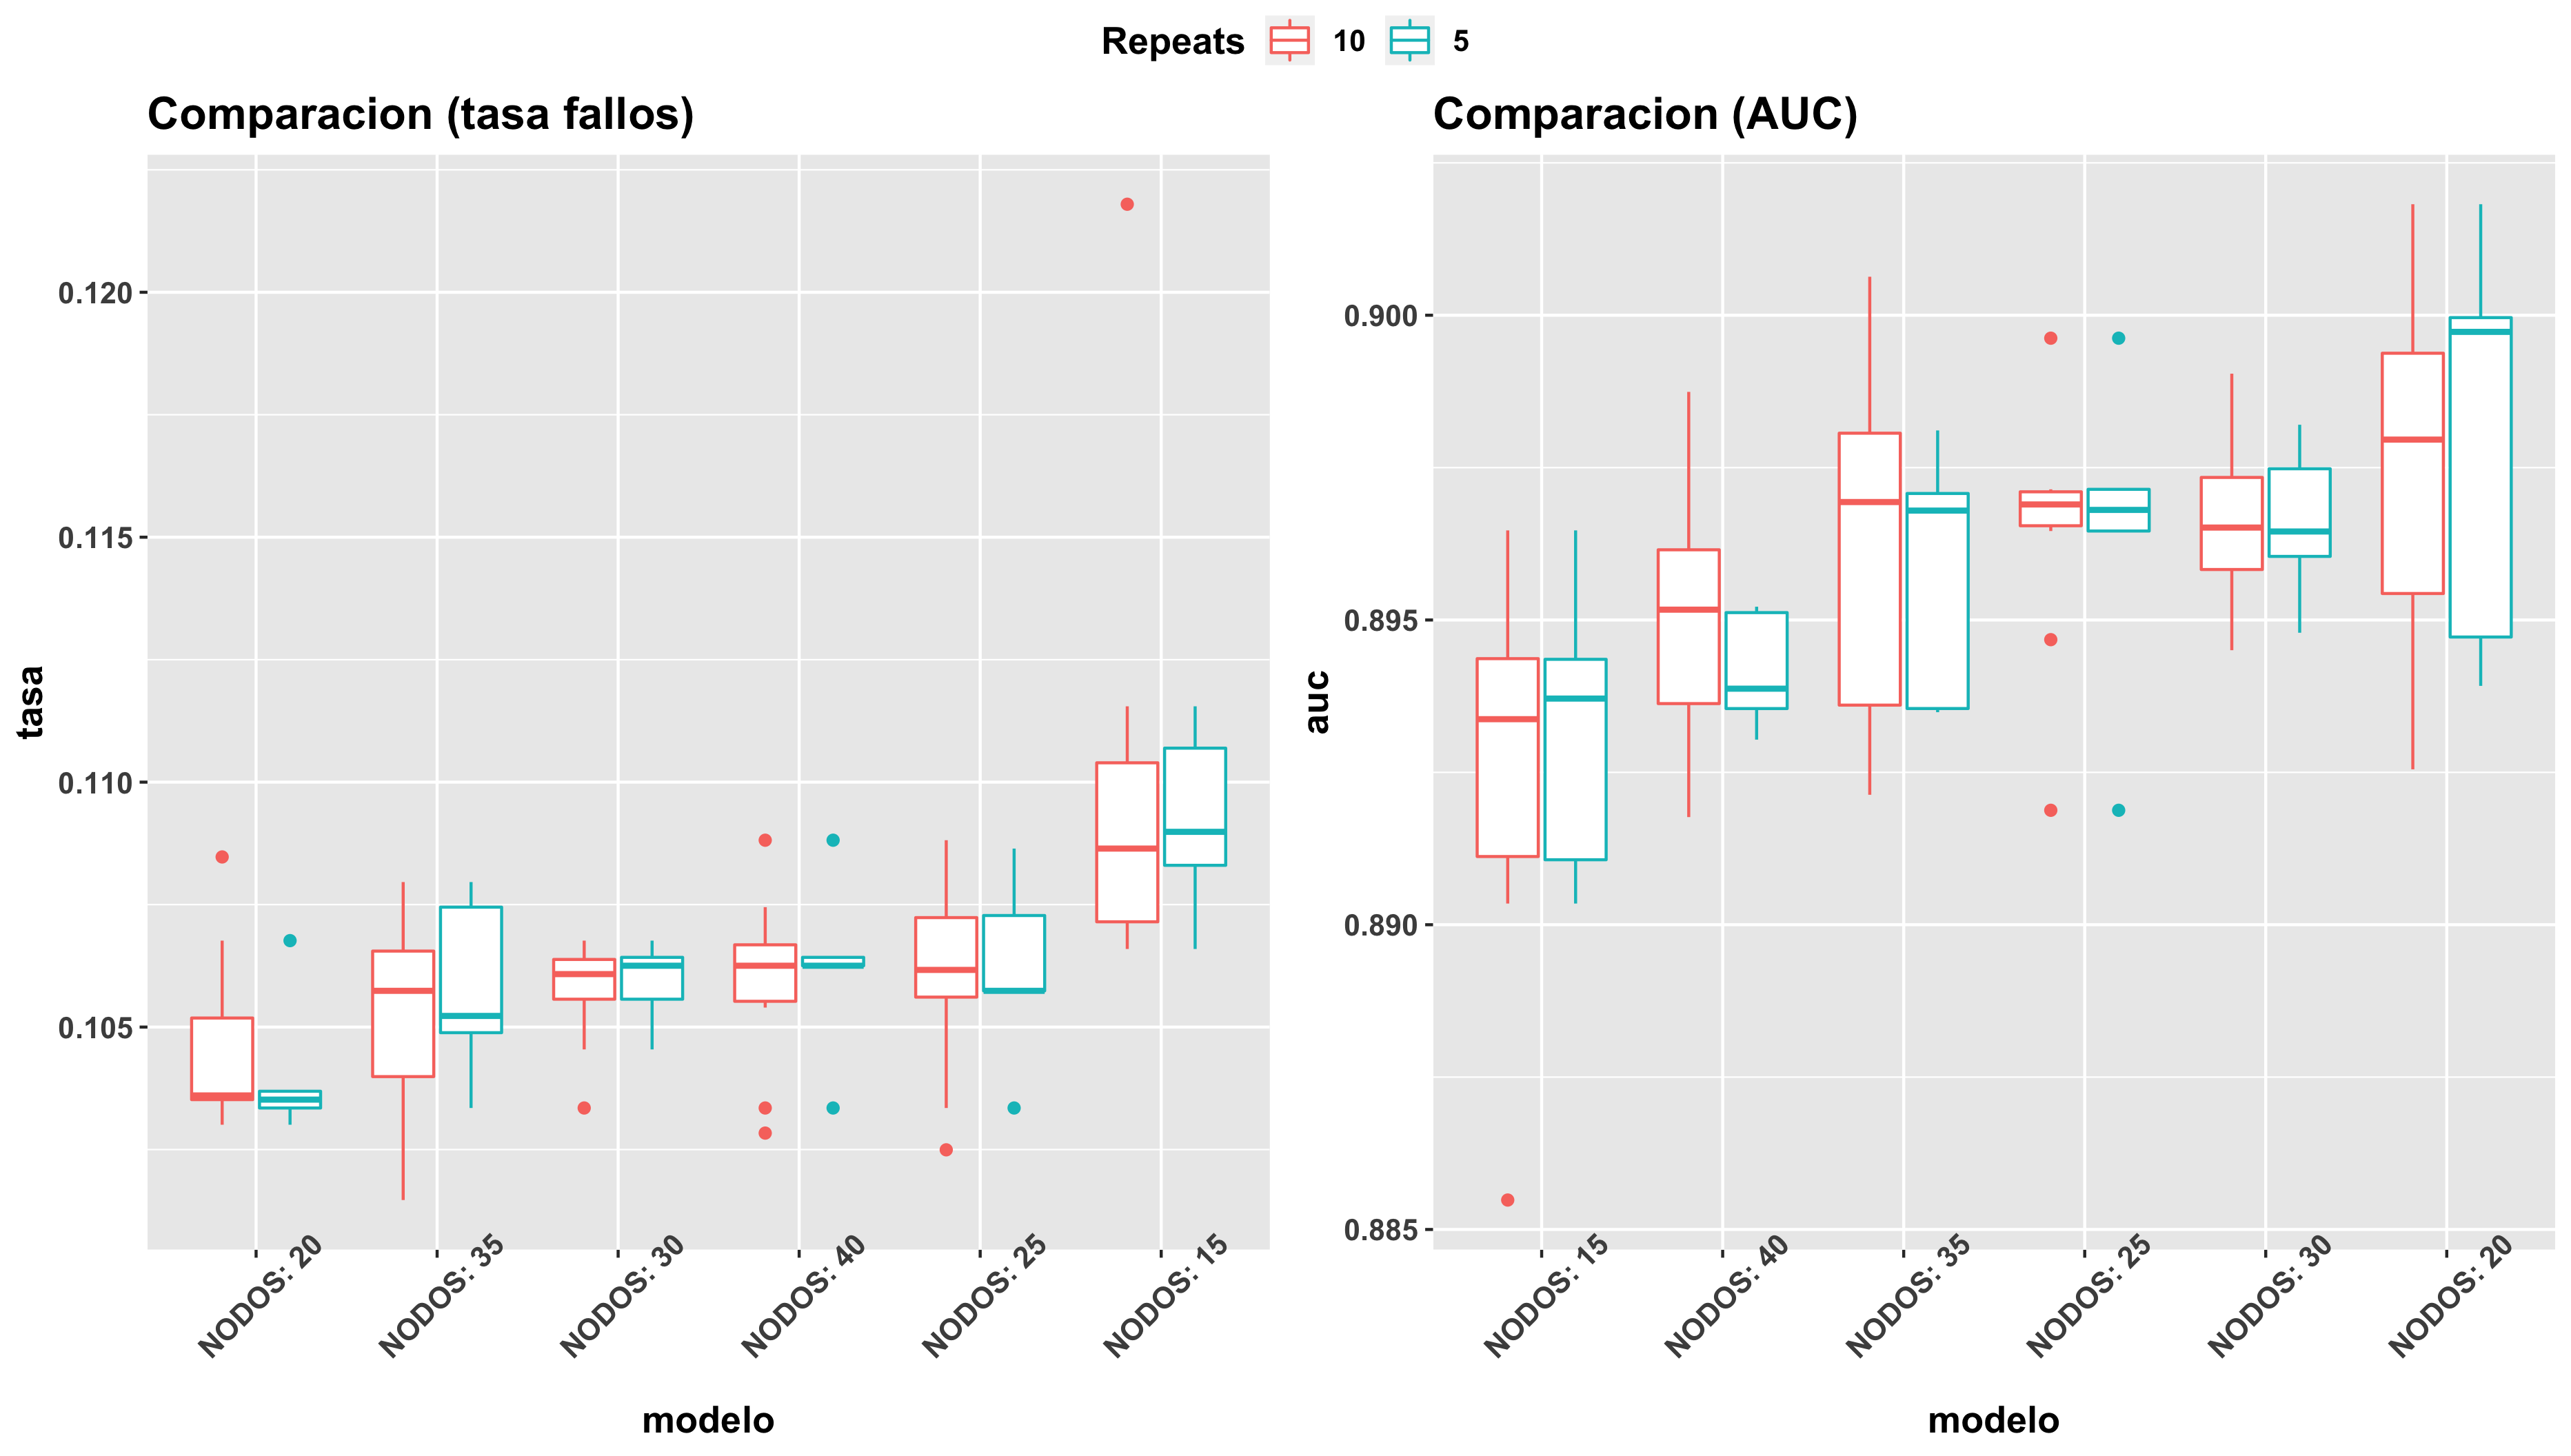
\includegraphics[width=0.99\linewidth,height=0.99\textheight,]{./charts/02_comparacion_tasa_auc_modelo1_10rep} 

}

\caption{Comparacion avnnet modelo 1 (10 rep.)}\label{fig:unnamed-chunk-53}
\end{figure}

Comprobamos que tanto el orden de los diferentes modelos como su
varianza se mantienen prácticamente constante. En conclusión, con el
primer \emph{set} de variables \textbf{nos decantamos por un modelo de
red con 15 nodos}, dado que la ganancia que supone al aumentar el número
de nodos, tanto en AUC como en tasa de fallos, es muy pequeña.

A continuación, y aumentando a 10 el número de repeticiones, tuneamos el
número de iteraciones:

\begin{figure}[h!]

{\centering 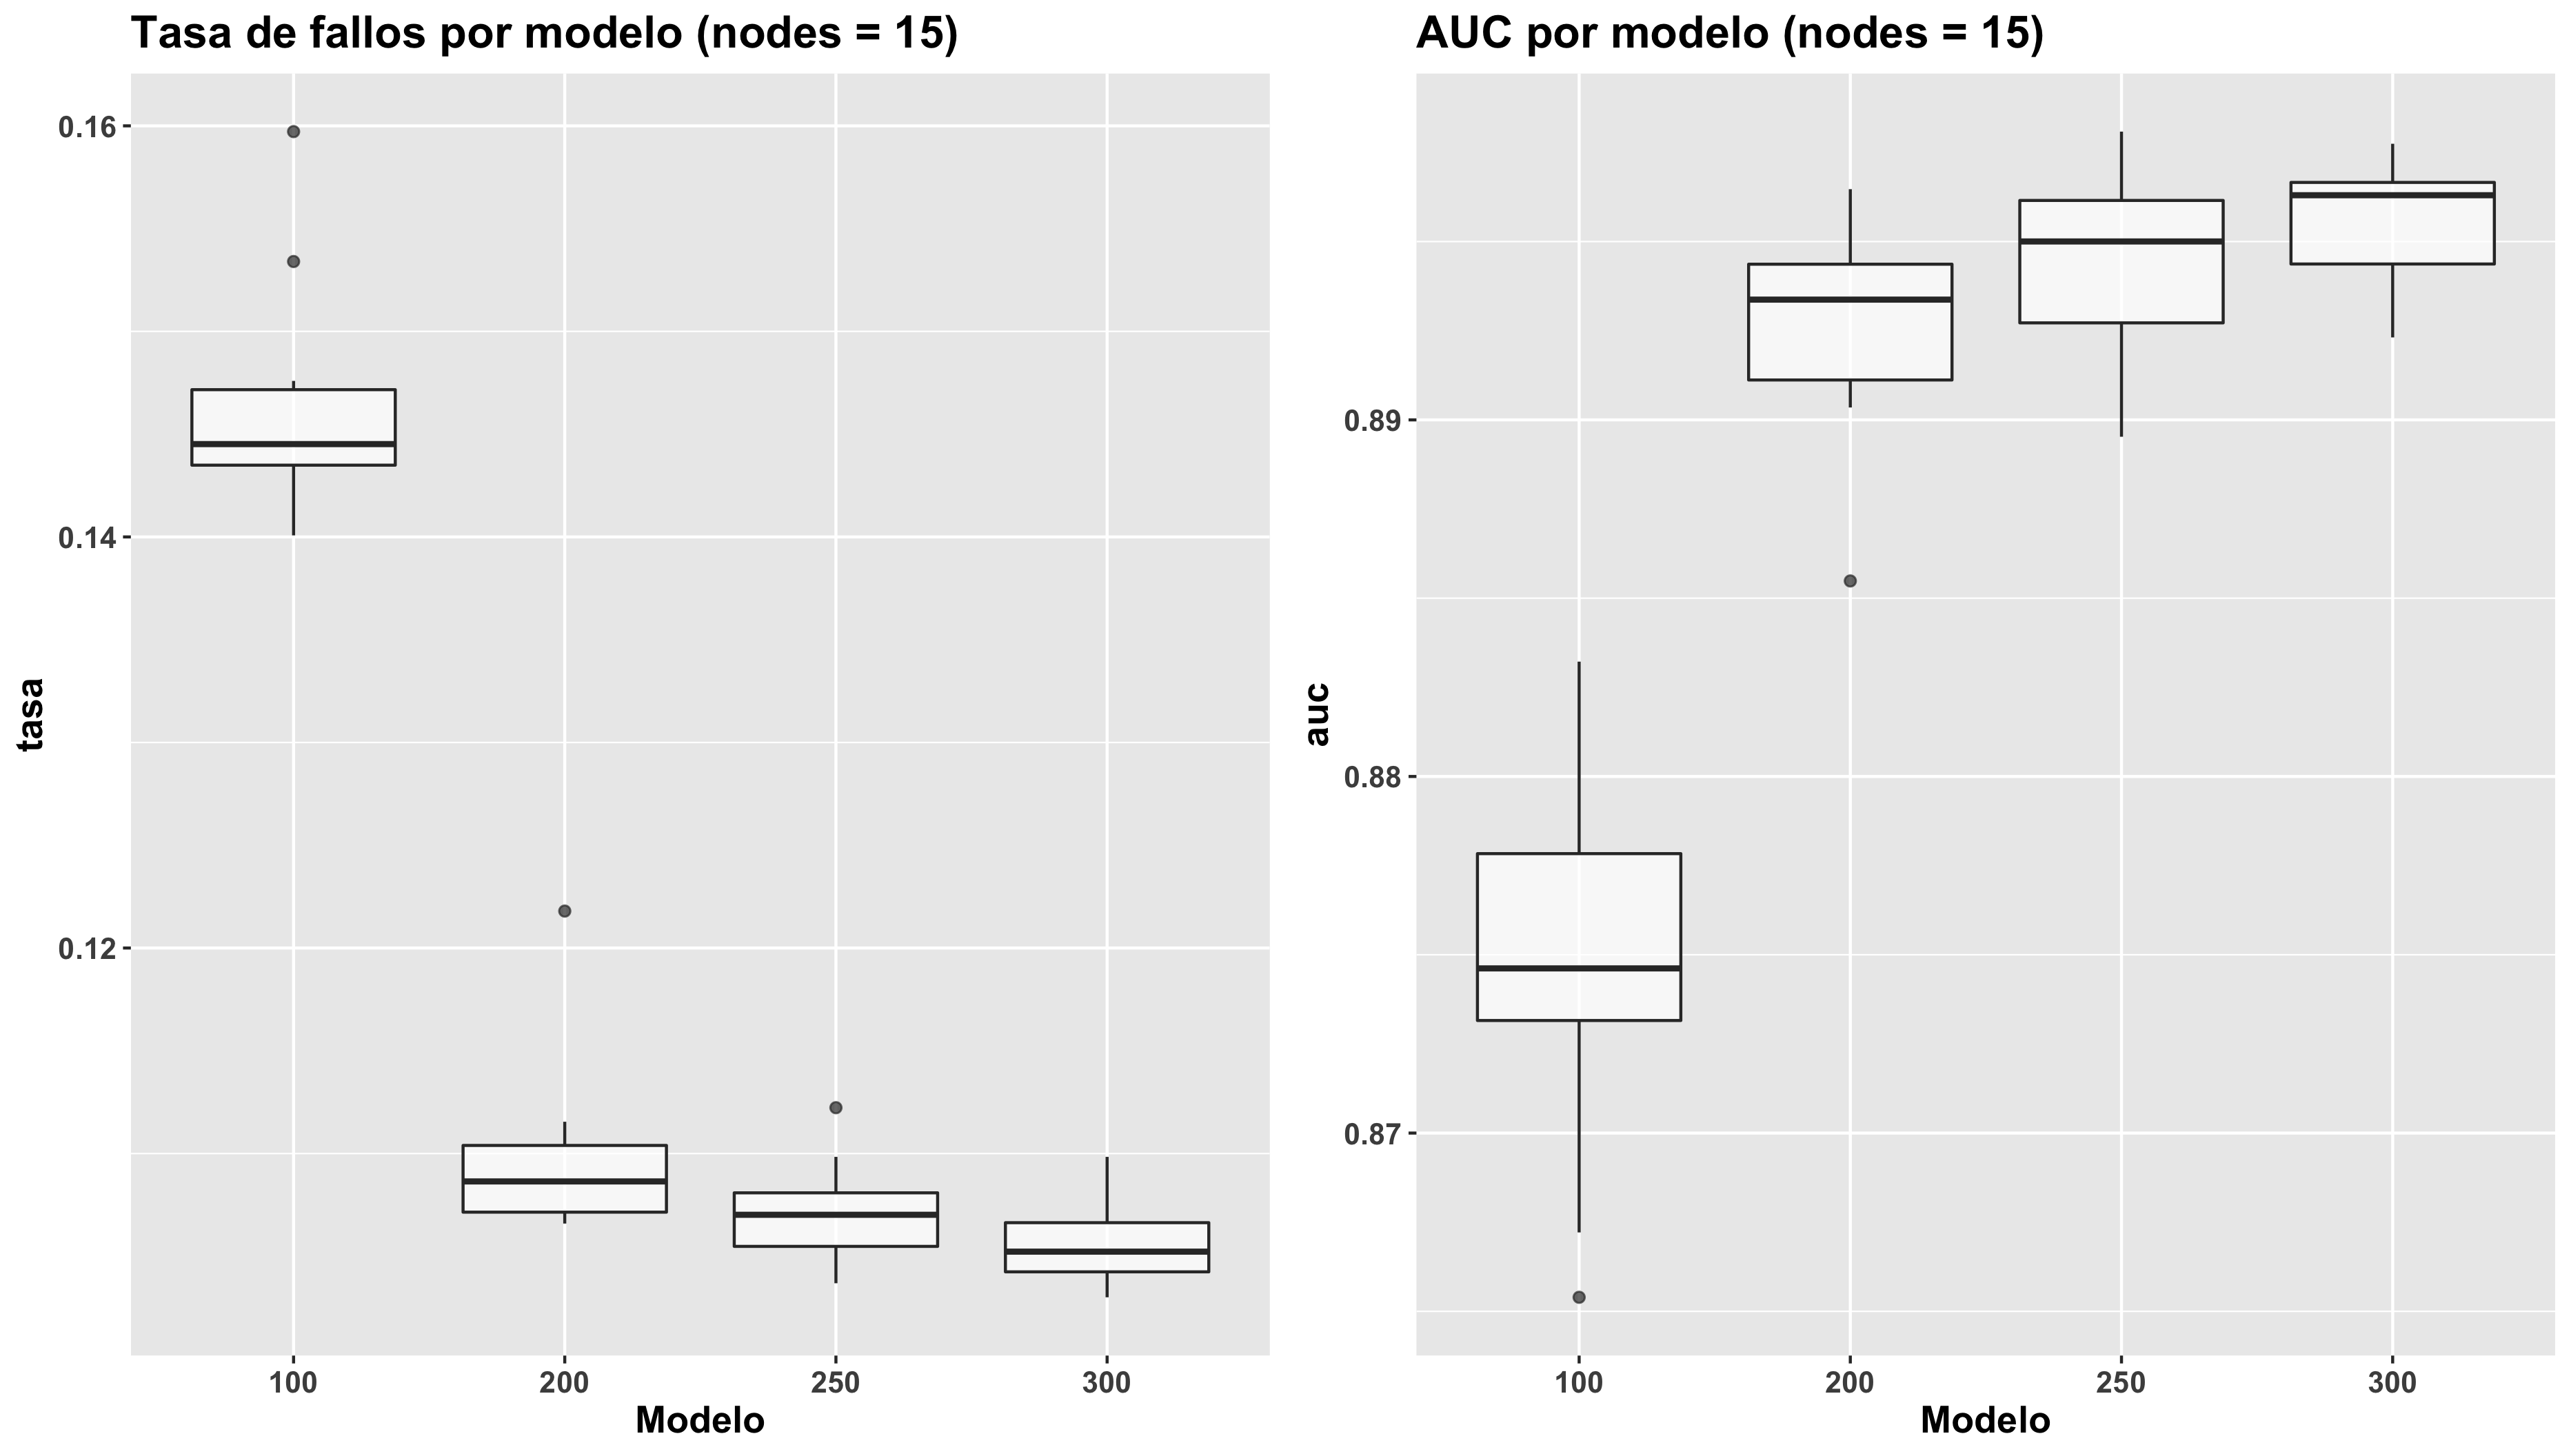
\includegraphics[width=0.99\linewidth,height=0.99\textheight,]{./charts/02_comparacion_tasa_auc_modelo1_10rep_iters} 

}

\caption{Comparacion avnnet modelo 1 (iteraciones)}\label{fig:unnamed-chunk-54}
\end{figure}

Analizando los resultados, \textbf{bien es cierto que conforme aumenta
el número de iteraciones, tanto la tasa de fallos como el AUC comienzan
a estabilizarse}. No obstante, la ganancia que supone aumentar el número
de iteraciones es muy pequeña. A modo de ejemplo, de 200 a 300
iteraciones, la tasa de fallos mejora de 0.11 a 0.105, aproximadamente,
mientras que el valor AUC apenas se ve afectado. Por tanto,
\textbf{mantenemos el número de iteraciones a 200}.

\hypertarget{modelo-2-aic-bic-top-4-1}{%
\subsection{6.2 Modelo 2 (AIC-BIC TOP
4)}\label{modelo-2-aic-bic-top-4-1}}

A continuación, realizamos los mismos pasos con el segundo \emph{set} de
variables candidato. En primer lugar, y dado que disponemos de 4
variables \emph{input}, para obtener 20 o 30 observaciones por
parámetros necesitamos:

\begin{enumerate}
\def\labelenumi{\arabic{enumi}.}
\tightlist
\item
  Con 20 observaciones por parámetro:
\end{enumerate}

\[
\text{Con } k = 4 \text{ variables input, entonces: } 6 * h + 1 = 292. \text{ Es decir}, 48-49 \text{ nodos}
\]

\begin{enumerate}
\def\labelenumi{\arabic{enumi}.}
\setcounter{enumi}{1}
\tightlist
\item
  Con 30 observaciones por parámetro: \[
  \text{Con } k = 4 \text{ variables input, entonces: } 6 * h + 1 = 195 \text{. Es decir}, 27-28 \text{ nodos}
  \]
\end{enumerate}

Con un primer cálculo, necesitaríamos un elevado número de nodos para
obtener, al menos, 20 o 30 observaciones por parámetro. Sin embargo, si
nos fijamos en lo empírico:

\begin{Shaded}
\begin{Highlighting}[]
\NormalTok{size.candidato}\FloatTok{.2}\NormalTok{ <{-}}\StringTok{ }\KeywordTok{c}\NormalTok{(}\DecValTok{5}\NormalTok{, }\DecValTok{10}\NormalTok{, }\DecValTok{15}\NormalTok{, }\DecValTok{20}\NormalTok{, }\DecValTok{25}\NormalTok{, }\DecValTok{30}\NormalTok{, }\DecValTok{35}\NormalTok{, }\DecValTok{40}\NormalTok{, }\DecValTok{45}\NormalTok{)}
\NormalTok{decay.candidato}\FloatTok{.2}\NormalTok{ <{-}}\StringTok{ }\KeywordTok{c}\NormalTok{(}\FloatTok{0.1}\NormalTok{, }\FloatTok{0.01}\NormalTok{, }\FloatTok{0.001}\NormalTok{)}

\NormalTok{cvnnet.candidato}\FloatTok{.1}\NormalTok{ <{-}}\StringTok{ }\KeywordTok{cruzadaavnnetbin}\NormalTok{(}\DataTypeTok{data=}\NormalTok{surgical\_dataset,}\DataTypeTok{vardep=}\NormalTok{target,}
                                       \DataTypeTok{listconti=}\NormalTok{var\_modelo2, }\DataTypeTok{listclass=}\KeywordTok{c}\NormalTok{(}\StringTok{""}\NormalTok{),}
                                       \DataTypeTok{grupos=}\DecValTok{5}\NormalTok{,}\DataTypeTok{sinicio=}\DecValTok{1234}\NormalTok{,}\DataTypeTok{repe=}\DecValTok{5}\NormalTok{, }\DataTypeTok{size=}\NormalTok{size.candidato}\FloatTok{.1}\NormalTok{,}
                                       \DataTypeTok{decay=}\NormalTok{decay.candidato}\FloatTok{.1}\NormalTok{,}\DataTypeTok{repeticiones=}\DecValTok{5}\NormalTok{,}\DataTypeTok{itera=}\DecValTok{200}\NormalTok{)}
\end{Highlighting}
\end{Shaded}

\begin{verbatim}
##    id size decay  Accuracy
## 1   1   20 0.001 0.9026305
## 2   2   35 0.001 0.9021868
## 3   3   25 0.001 0.9020152
## 4   4   30 0.001 0.9017081
## 5   5   25 0.010 0.9007853
## 6   6   30 0.010 0.8998632
## 7   7   15 0.001 0.8997609
## 8   8   45 0.001 0.8995550
## 9   9   20 0.010 0.8994869
## 10 10   45 0.010 0.8994521
## 11 11   40 0.001 0.8994190
## 12 12   15 0.010 0.8992479
## 13 13   35 0.010 0.8989061
## 14 14   40 0.010 0.8986332
## 15 15   10 0.010 0.8946358
## 16 16   10 0.001 0.8906726
## 17 17   25 0.100 0.8897164
## 18 18   40 0.100 0.8896133
## 19 19   20 0.100 0.8895444
## 20 20   35 0.100 0.8894082
## 21 21   30 0.100 0.8888957
## 22 22   45 0.100 0.8888273
## 23 23   15 0.100 0.8884856
## 24 24   10 0.100 0.8855818
## 25 25    5 0.010 0.8447890
## 26 26    5 0.001 0.8358688
## 27 27    5 0.100 0.8303017
\end{verbatim}

En un primer resultado, \textbf{con un parámetro de regularización
pequeño obtenemos buenos resultados}. A modo de ejemplo, llama la
atención modelos de red con 20, 25 o 30 nodos que alcanzan un
\emph{Accuracy} de 0.90. Sin embargo, conforme descendemos en la tabla
(y con ello, el número de nodos) comprobamos que la diferencia no es muy
significativa: con tan solo 15 o 10 nodos y un \emph{decay} de 0.01, el
valor de \emph{Accuracy} tan solo empeora en 0.89. Es decir, a simple
vista el hecho de aumentar el número de nodos \textbf{no compensa la
ganancia de \emph{Accuracy}}.

No obstante, analicemos tanto el sesgo como la varianza con los mejores
modelos:

\begin{Shaded}
\begin{Highlighting}[]
\CommentTok{\# Probamos con 15{-}20{-}25{-}30 nodos y decay 0.001; 10{-}15 nodos y decay 0.01}
\NormalTok{size.candidato}\FloatTok{.2}\NormalTok{  <{-}}\StringTok{ }\KeywordTok{c}\NormalTok{(}\DecValTok{10}\NormalTok{, }\DecValTok{15}\NormalTok{, }\DecValTok{15}\NormalTok{, }\DecValTok{20}\NormalTok{, }\DecValTok{25}\NormalTok{, }\DecValTok{30}\NormalTok{)}
\NormalTok{decay.candidato}\FloatTok{.2}\NormalTok{ <{-}}\StringTok{ }\KeywordTok{c}\NormalTok{(}\FloatTok{0.01}\NormalTok{, }\FloatTok{0.01}\NormalTok{, }\FloatTok{0.001}\NormalTok{, }\FloatTok{0.001}\NormalTok{, }\FloatTok{0.001}\NormalTok{, }\FloatTok{0.001}\NormalTok{)}
\end{Highlighting}
\end{Shaded}

\begin{figure}[h!]

{\centering 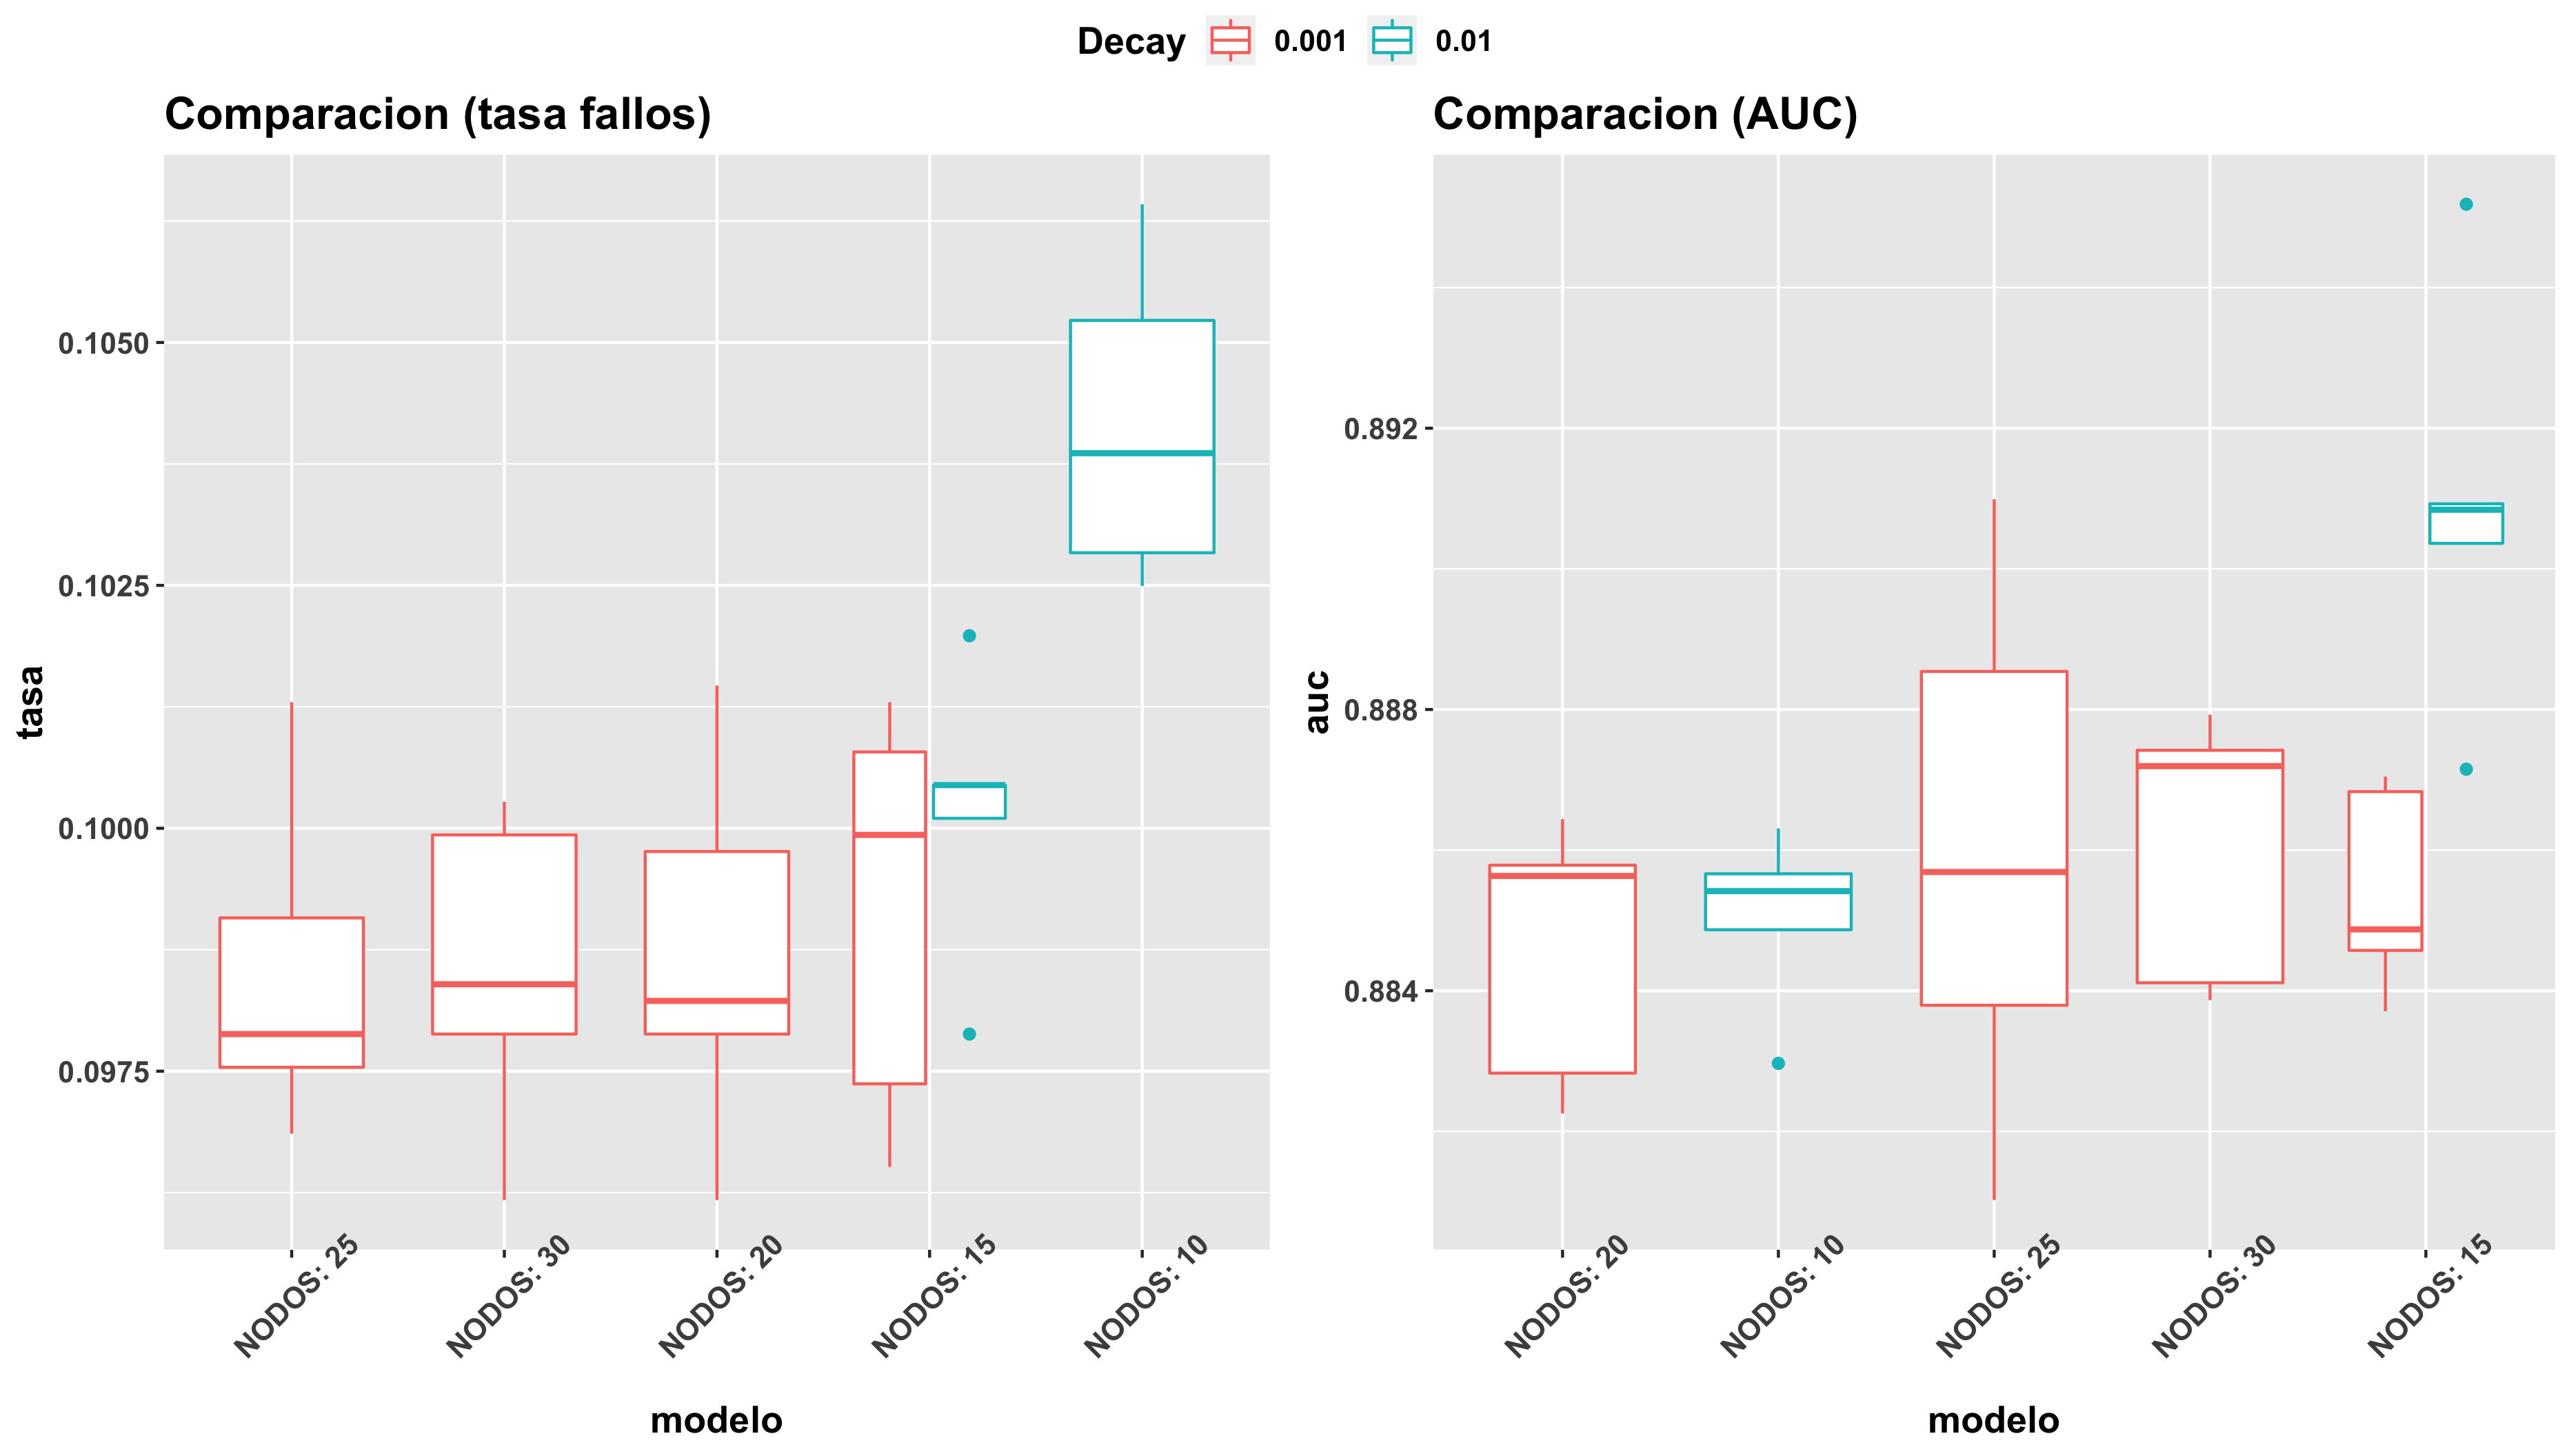
\includegraphics[width=0.99\linewidth,height=0.99\textheight,]{./charts/02_comparacion_tasa_auc_modelo2_5rep} 

}

\caption{Comparacion avnnet modelo 2}\label{fig:unnamed-chunk-58}
\end{figure}

En un primer resultado, \textbf{la ganancia de error que supone reducir
el número de nodos a 10 (y con un \emph{decay} de 0.01), es muy pequeña:
de 0.09 con 25 nodos a 0.105 con tan solo 10 nodos}. Del mismo modo
sucede con el área bajo la curva, donde la mejora con 15 o 30 nodos es
de tan solo unas milésimas de diferencia, lo cual puede depender de
condiciones azarosas como la semilla de aleatoriedad. No obstante, con
10, 15 y 20 nodos, echemos un vistazo al modelo con 10 repeticiones:

\begin{figure}[h!]

{\centering 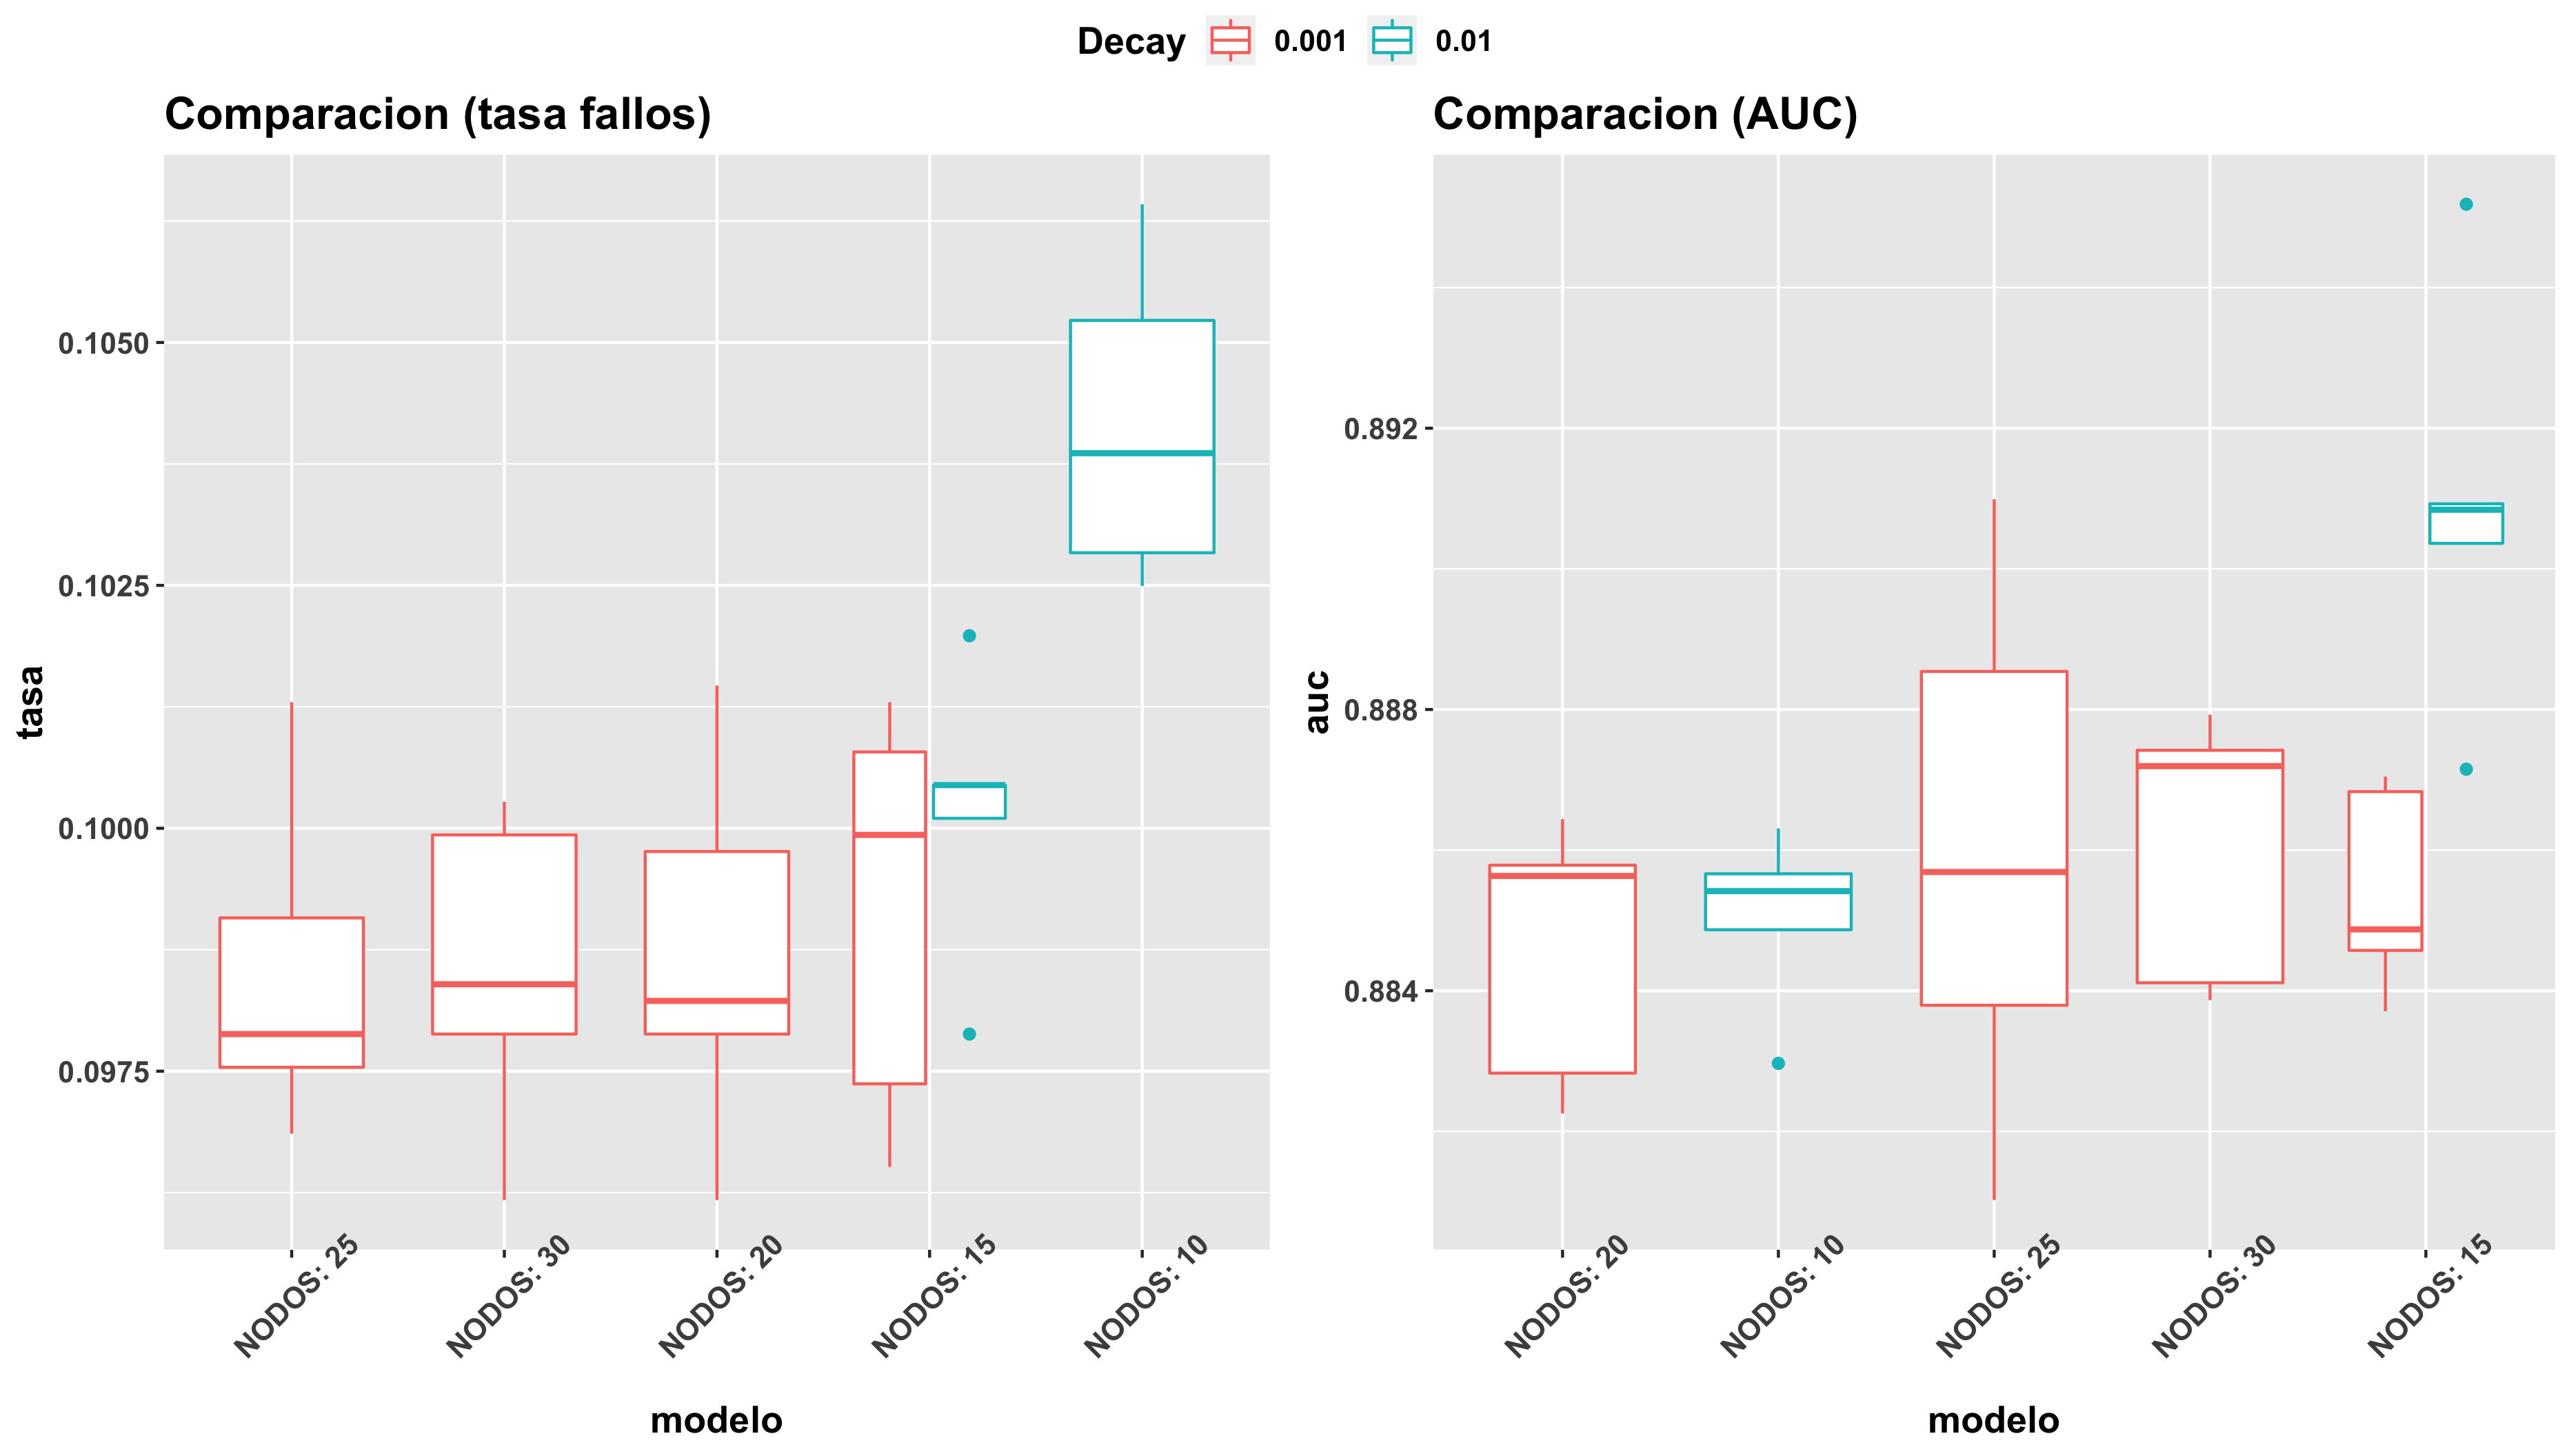
\includegraphics[width=0.99\linewidth,height=0.99\textheight,]{./charts/02_comparacion_tasa_auc_modelo2_5rep} 

}

\caption{Comparacion avnnet modelo 2 (10 rep.)}\label{fig:unnamed-chunk-59}
\end{figure}

Incluso aumentando a 10 repeticiones, el orden de los modelos no cambia.
Por tanto, dada su simplicidad y la poca ganancia de error que supone,
\textbf{elegimos el modelo con 10 nodos y \emph{decay} 0.01}.

Por último, tuneamos el número de iteraciones:

\begin{figure}[h!]

{\centering 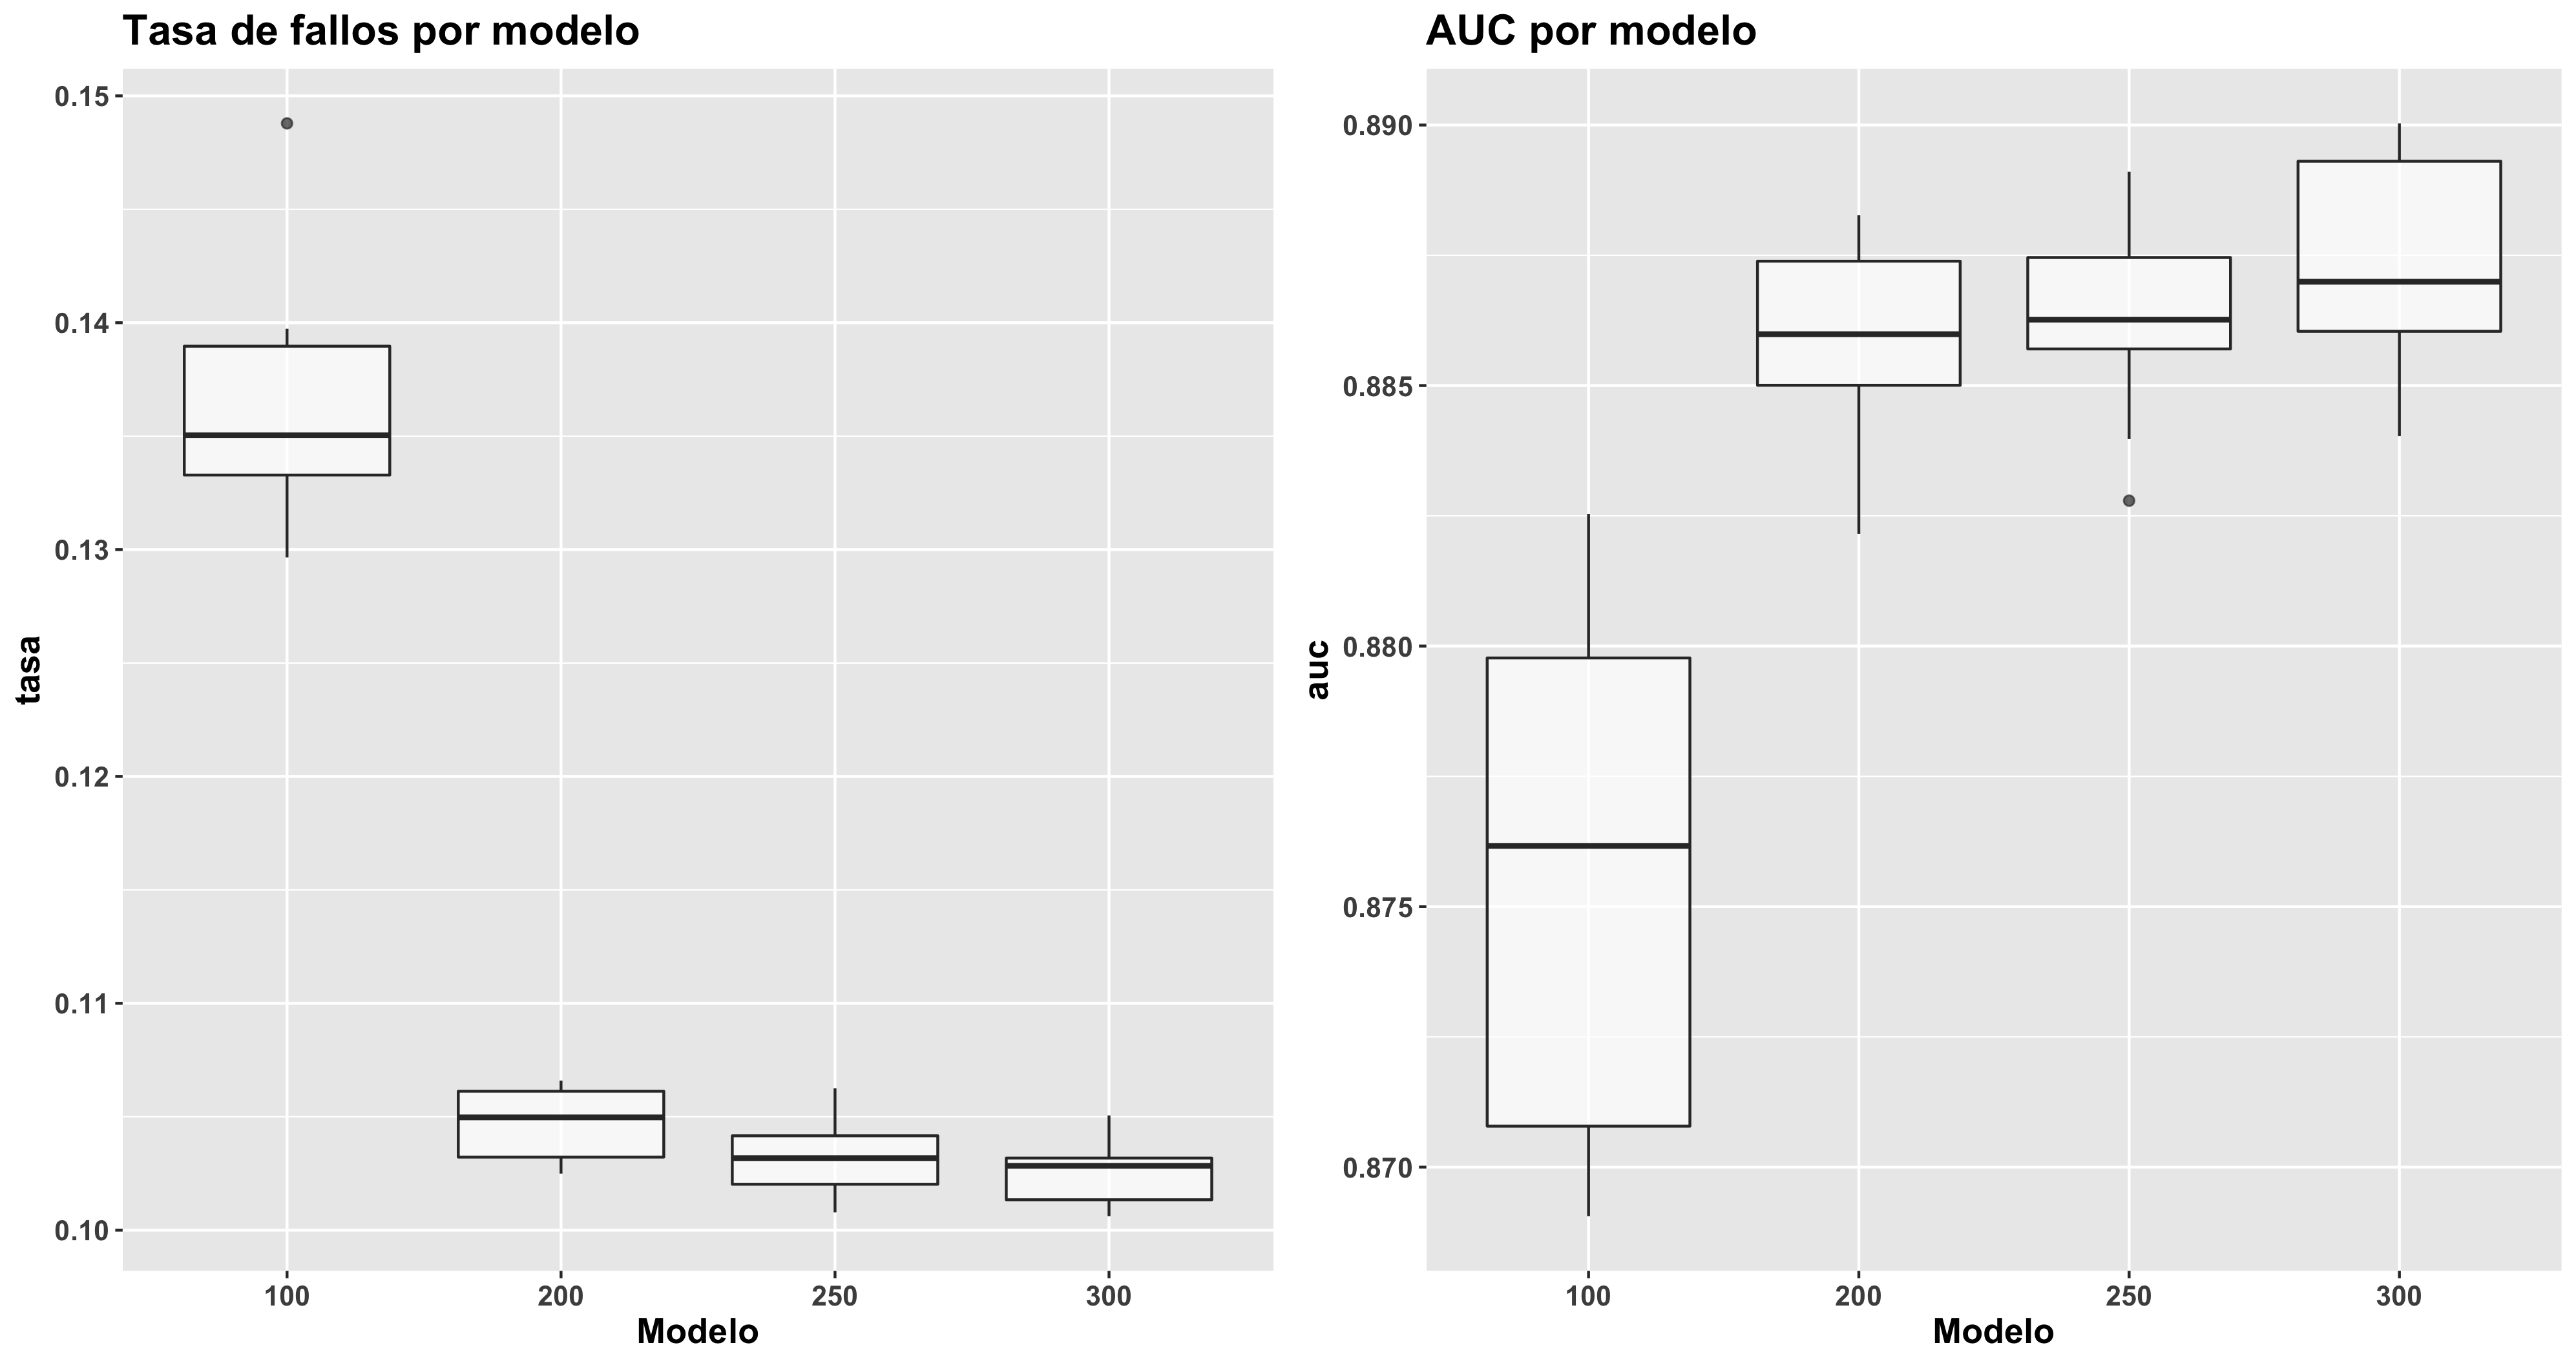
\includegraphics[width=0.99\linewidth,height=0.99\textheight,]{./charts/02_comparacion_tasa_auc_modelo2_10rep_iters} 

}

\caption{Comparacion avnnet modelo 2 (iteraciones)}\label{fig:unnamed-chunk-60}
\end{figure}

Del mismo modo que sucedía con el primer \emph{set} de variables,
\textbf{aumentar el número de iteraciones no supone una mejoría
significativa}, por lo que lo mantenemos a 200.

\hypertarget{comparaciuxf3n-final}{%
\subsection{6.3 Comparación final}\label{comparaciuxf3n-final}}

Una vez obtenidos ambos modelos, con los datos \emph{test} realizamos
las primeras predicciones:

\begin{verbatim}
##                 modelo precision sensibilidad especificidad valor_pred_pos
## 1 Modelo 1 (BIC TOP 5)    0.8992       0.9471        0.8897         0.6305
## 2     Modelo 2 (top 4)    0.9032       0.9639        0.8913         0.6351
##   valor_pred_neg
## 1         0.9883
## 2         0.9921
\end{verbatim}

En primera instancia, \textbf{con un modelo de red sencillo conseguimos
mejorar prácticamente en todos los aspectos}. No obstante, cabe destacar
el valor predictivo positivo, que pese a su mejoría (del 20-30 al 63
\%), \textbf{continua existiendo un alto porcentaje de falsos
positivos}.

En conclusión, a la vista de los resultados obtenidos, tanto en tasa de
fallos como en AUC, \textbf{los modelos de red mejoran
significativamente los resultados del modelo}, un claro indicio de la
\textbf{no linealidad con la variable objetivo}. En relación con ambos
\emph{set} de variables, el hecho de añadir una variable \emph{input}
adicional en el primer modelo \textbf{no hace mejorar significativamente
sus resultados}:

\begin{figure}[h!]

{\centering 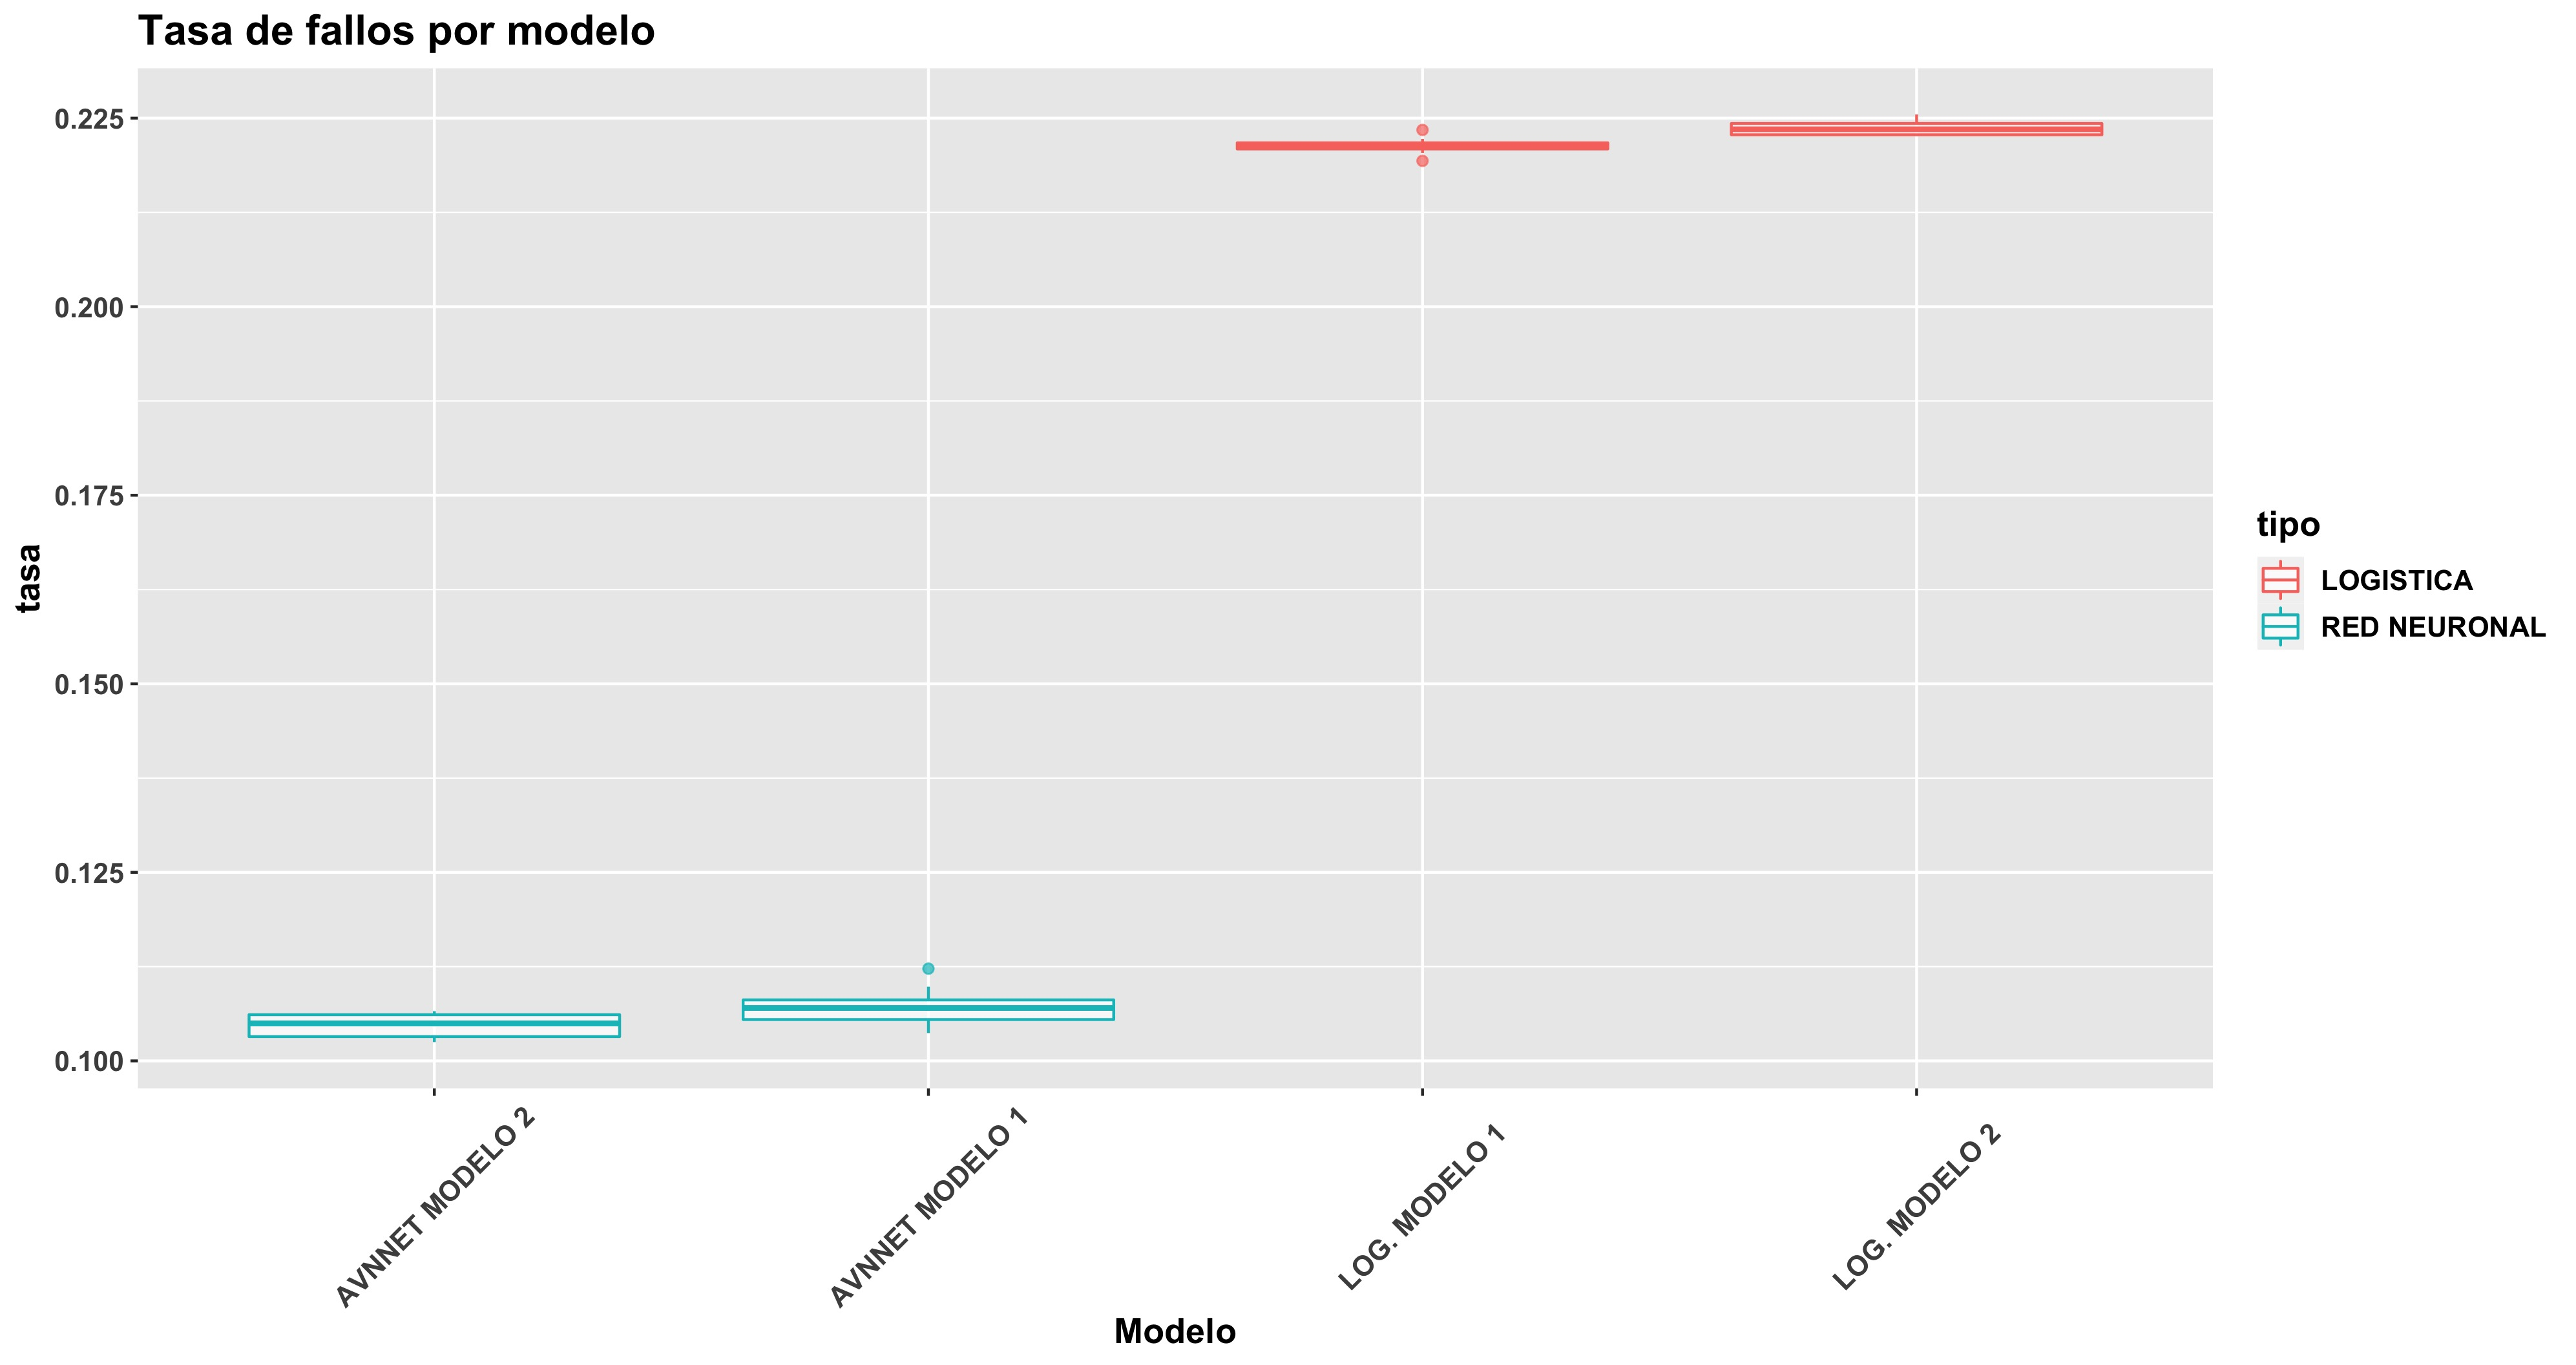
\includegraphics[width=0.99\linewidth,height=0.99\textheight,]{./charts/comparativas/02_log_avnnet_tasa} 

}

\caption{Comparacion tasa fallos log-avnnet}\label{fig:unnamed-chunk-62}
\end{figure}
\begin{figure}[h!]

{\centering 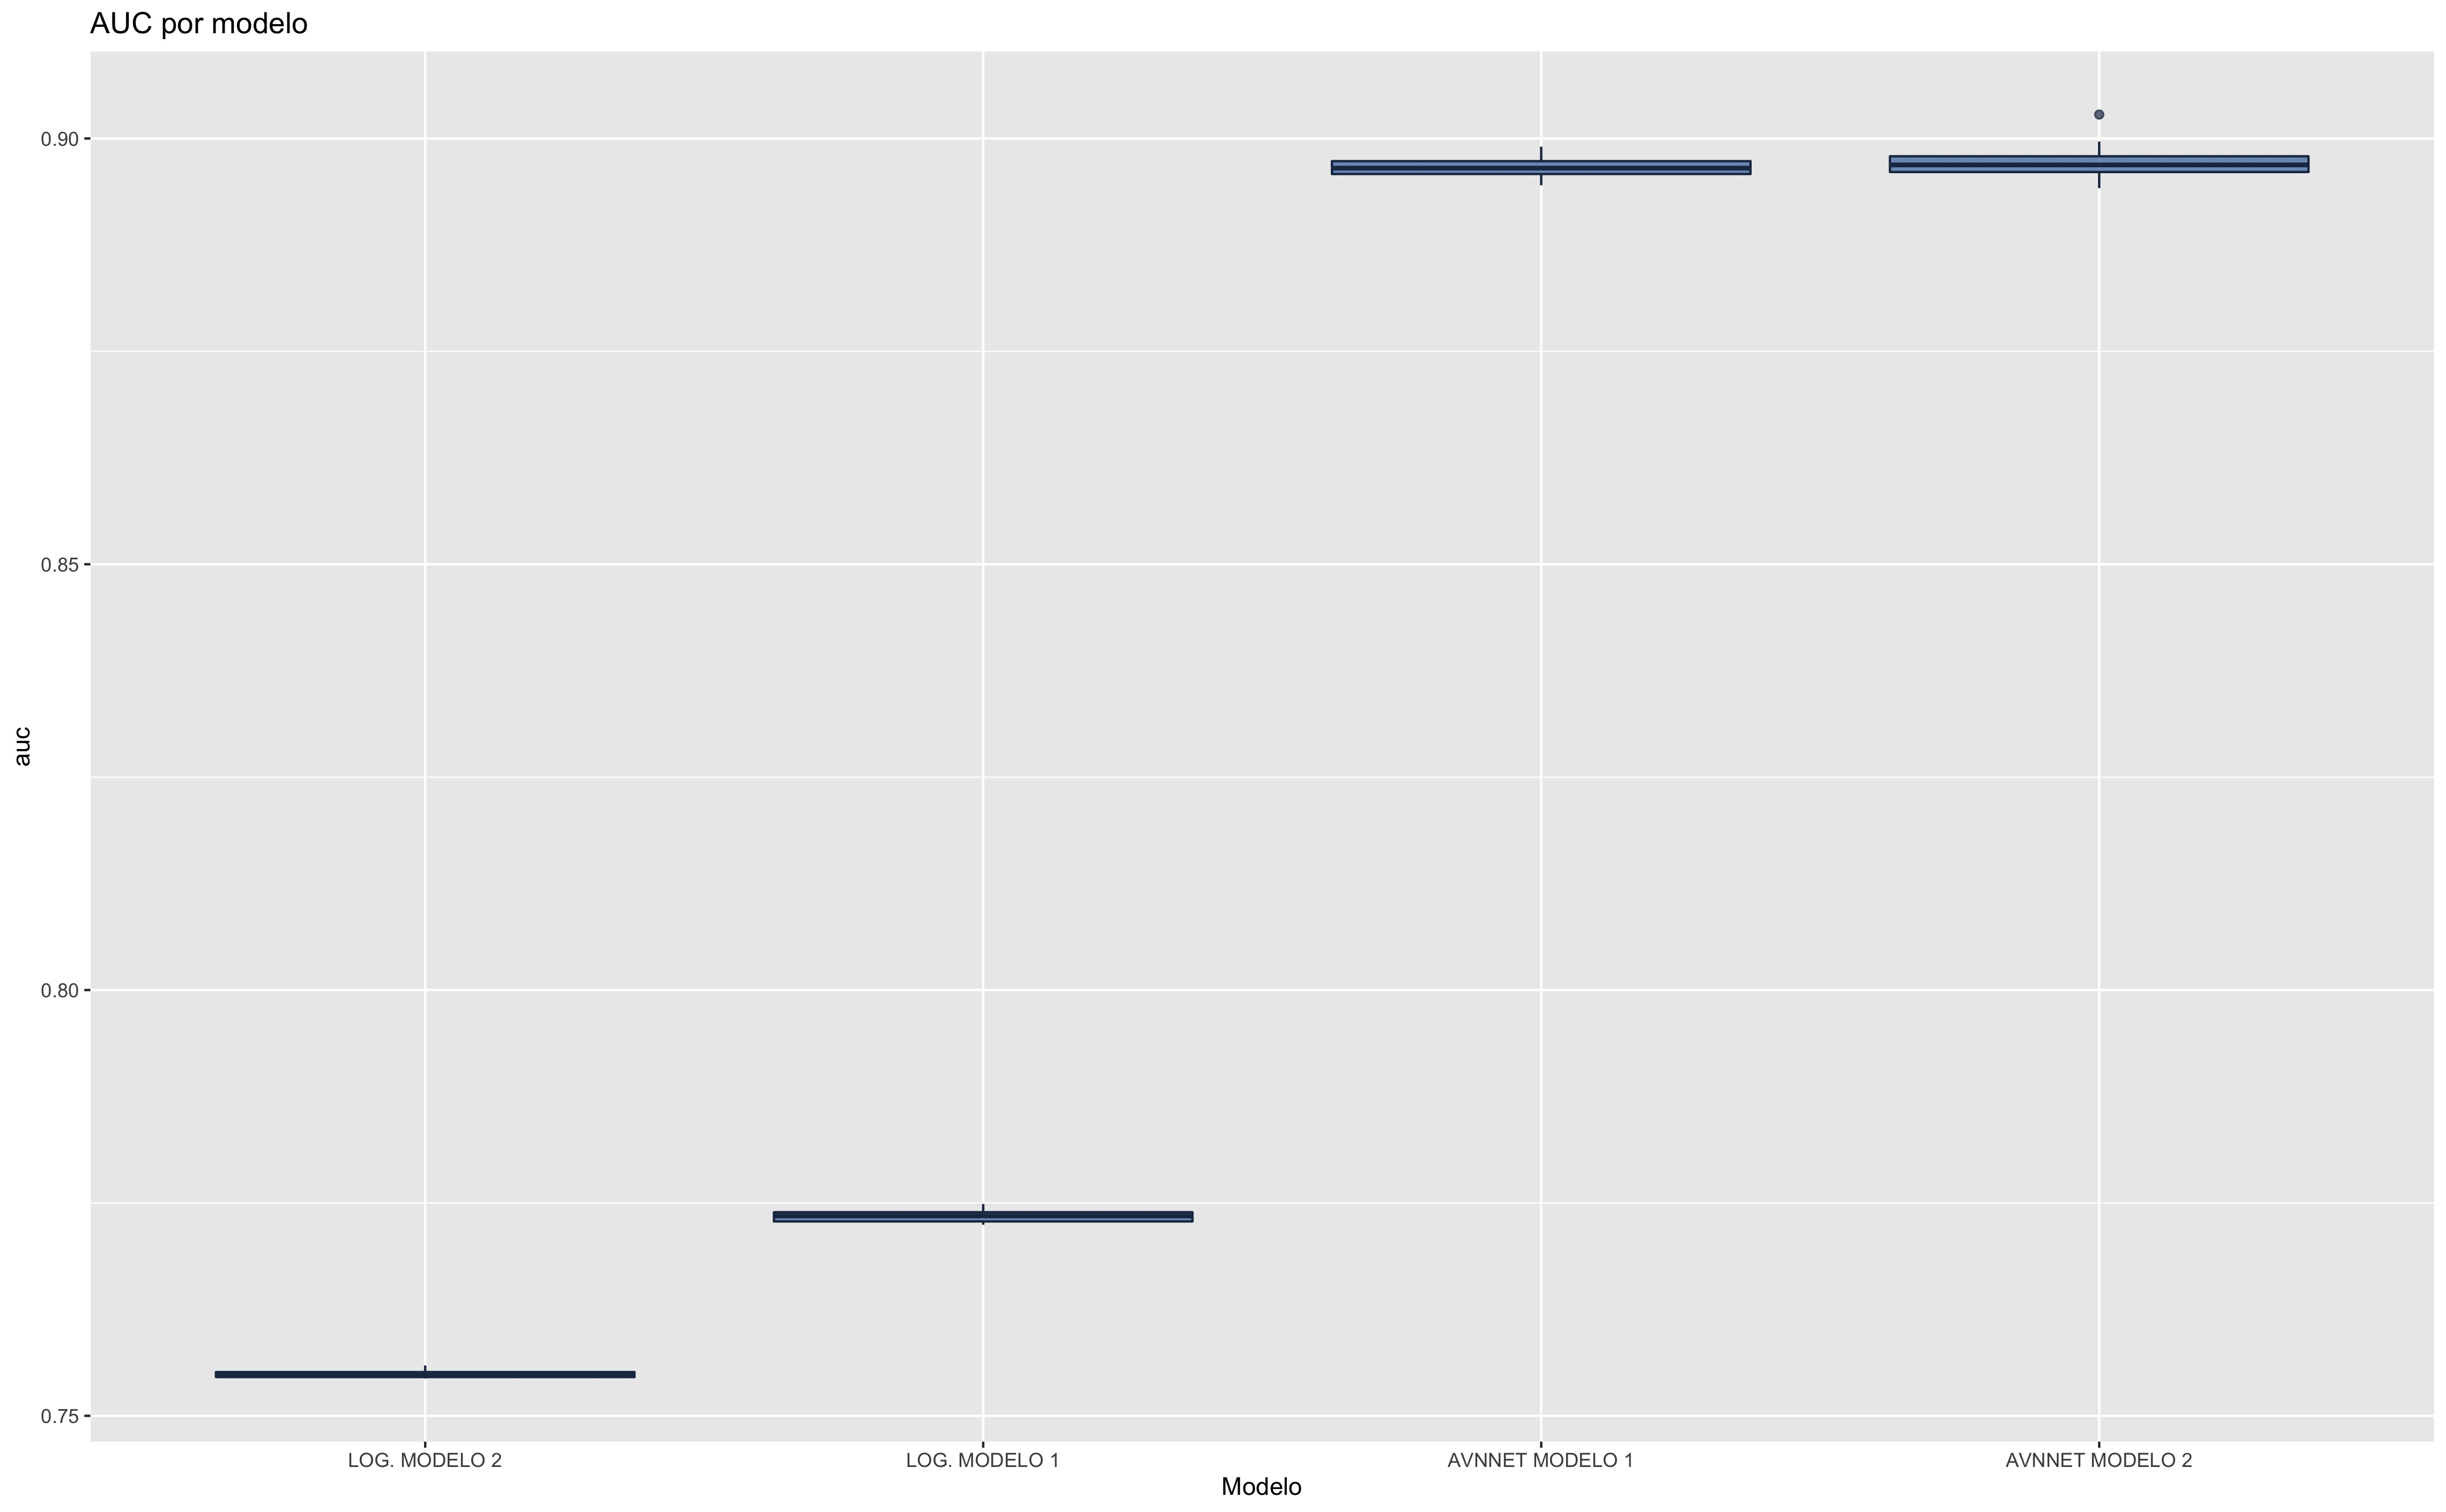
\includegraphics[width=0.99\linewidth,height=0.99\textheight,]{./charts/comparativas/02_log_avnnet_auc} 

}

\caption{Comparacion AUC log-avnnet}\label{fig:unnamed-chunk-63}
\end{figure}

\textbf{RESUMEN red neuronal}:

\begin{enumerate}
\def\labelenumi{\arabic{enumi}.}
\tightlist
\item
  modelo 1: \emph{size} = 15 y \emph{decay} = 0.01.
\item
  modelo 2: \emph{size} = 10 y \emph{decay} = 0.01.
\end{enumerate}

\hypertarget{bagging}{%
\section{7. Bagging}\label{bagging}}

\hypertarget{selecciuxf3n-del-nuxfamero-de-uxe1rboles}{%
\subsection{7.1 Selección del número de
árboles}\label{selecciuxf3n-del-nuxfamero-de-uxe1rboles}}

Continuando con el modelo \emph{bagging}, de forma previa al tuneo de
hipérparametros, debemos fijar un número de árboles (ntrees) para ambos
\emph{sets} de variables, un valor mínimo a partir del cual el error OOB
( \emph{Out of bag error} ) se estabiliza:

\begin{Shaded}
\begin{Highlighting}[]
\CommentTok{\#{-}{-} Seleccion del numero de arboles}
\KeywordTok{set.seed}\NormalTok{(}\DecValTok{1234}\NormalTok{)}
\CommentTok{\#{-}{-} Modelo 1}
\NormalTok{rfbis}\FloatTok{.1}\NormalTok{<{-}}\KeywordTok{randomForest}\NormalTok{(}\KeywordTok{factor}\NormalTok{(target)}\OperatorTok{\textasciitilde{}}\NormalTok{mortality\_rsi}\OperatorTok{+}\NormalTok{ccsMort30Rate}\OperatorTok{+}\NormalTok{bmi}\OperatorTok{+}\NormalTok{month}\FloatTok{.8}\OperatorTok{+}\NormalTok{Age,}
                      \DataTypeTok{data=}\NormalTok{surgical\_dataset,}
                      \DataTypeTok{mtry=}\NormalTok{mtry}\FloatTok{.1}\NormalTok{,}\DataTypeTok{ntree=}\DecValTok{5000}\NormalTok{,}\DataTypeTok{nodesize=}\DecValTok{10}\NormalTok{,}\DataTypeTok{replace=}\OtherTok{TRUE}\NormalTok{)}

\CommentTok{\#{-}{-} Modelo 2}
\NormalTok{rfbis}\FloatTok{.2}\NormalTok{<{-}}\KeywordTok{randomForest}\NormalTok{(}\KeywordTok{factor}\NormalTok{(target)}\OperatorTok{\textasciitilde{}}\NormalTok{Age}\OperatorTok{+}\NormalTok{mortality\_rsi}\OperatorTok{+}\NormalTok{bmi}\OperatorTok{+}\NormalTok{month}\FloatTok{.8}\NormalTok{,}
                      \DataTypeTok{data=}\NormalTok{surgical\_dataset,}
                      \DataTypeTok{mtry=}\NormalTok{mtry}\FloatTok{.2}\NormalTok{,}\DataTypeTok{ntree=}\DecValTok{5000}\NormalTok{,}\DataTypeTok{nodesize=}\DecValTok{10}\NormalTok{,}\DataTypeTok{replace=}\OtherTok{TRUE}\NormalTok{)}
\end{Highlighting}
\end{Shaded}

\begin{figure}[h!]

{\centering 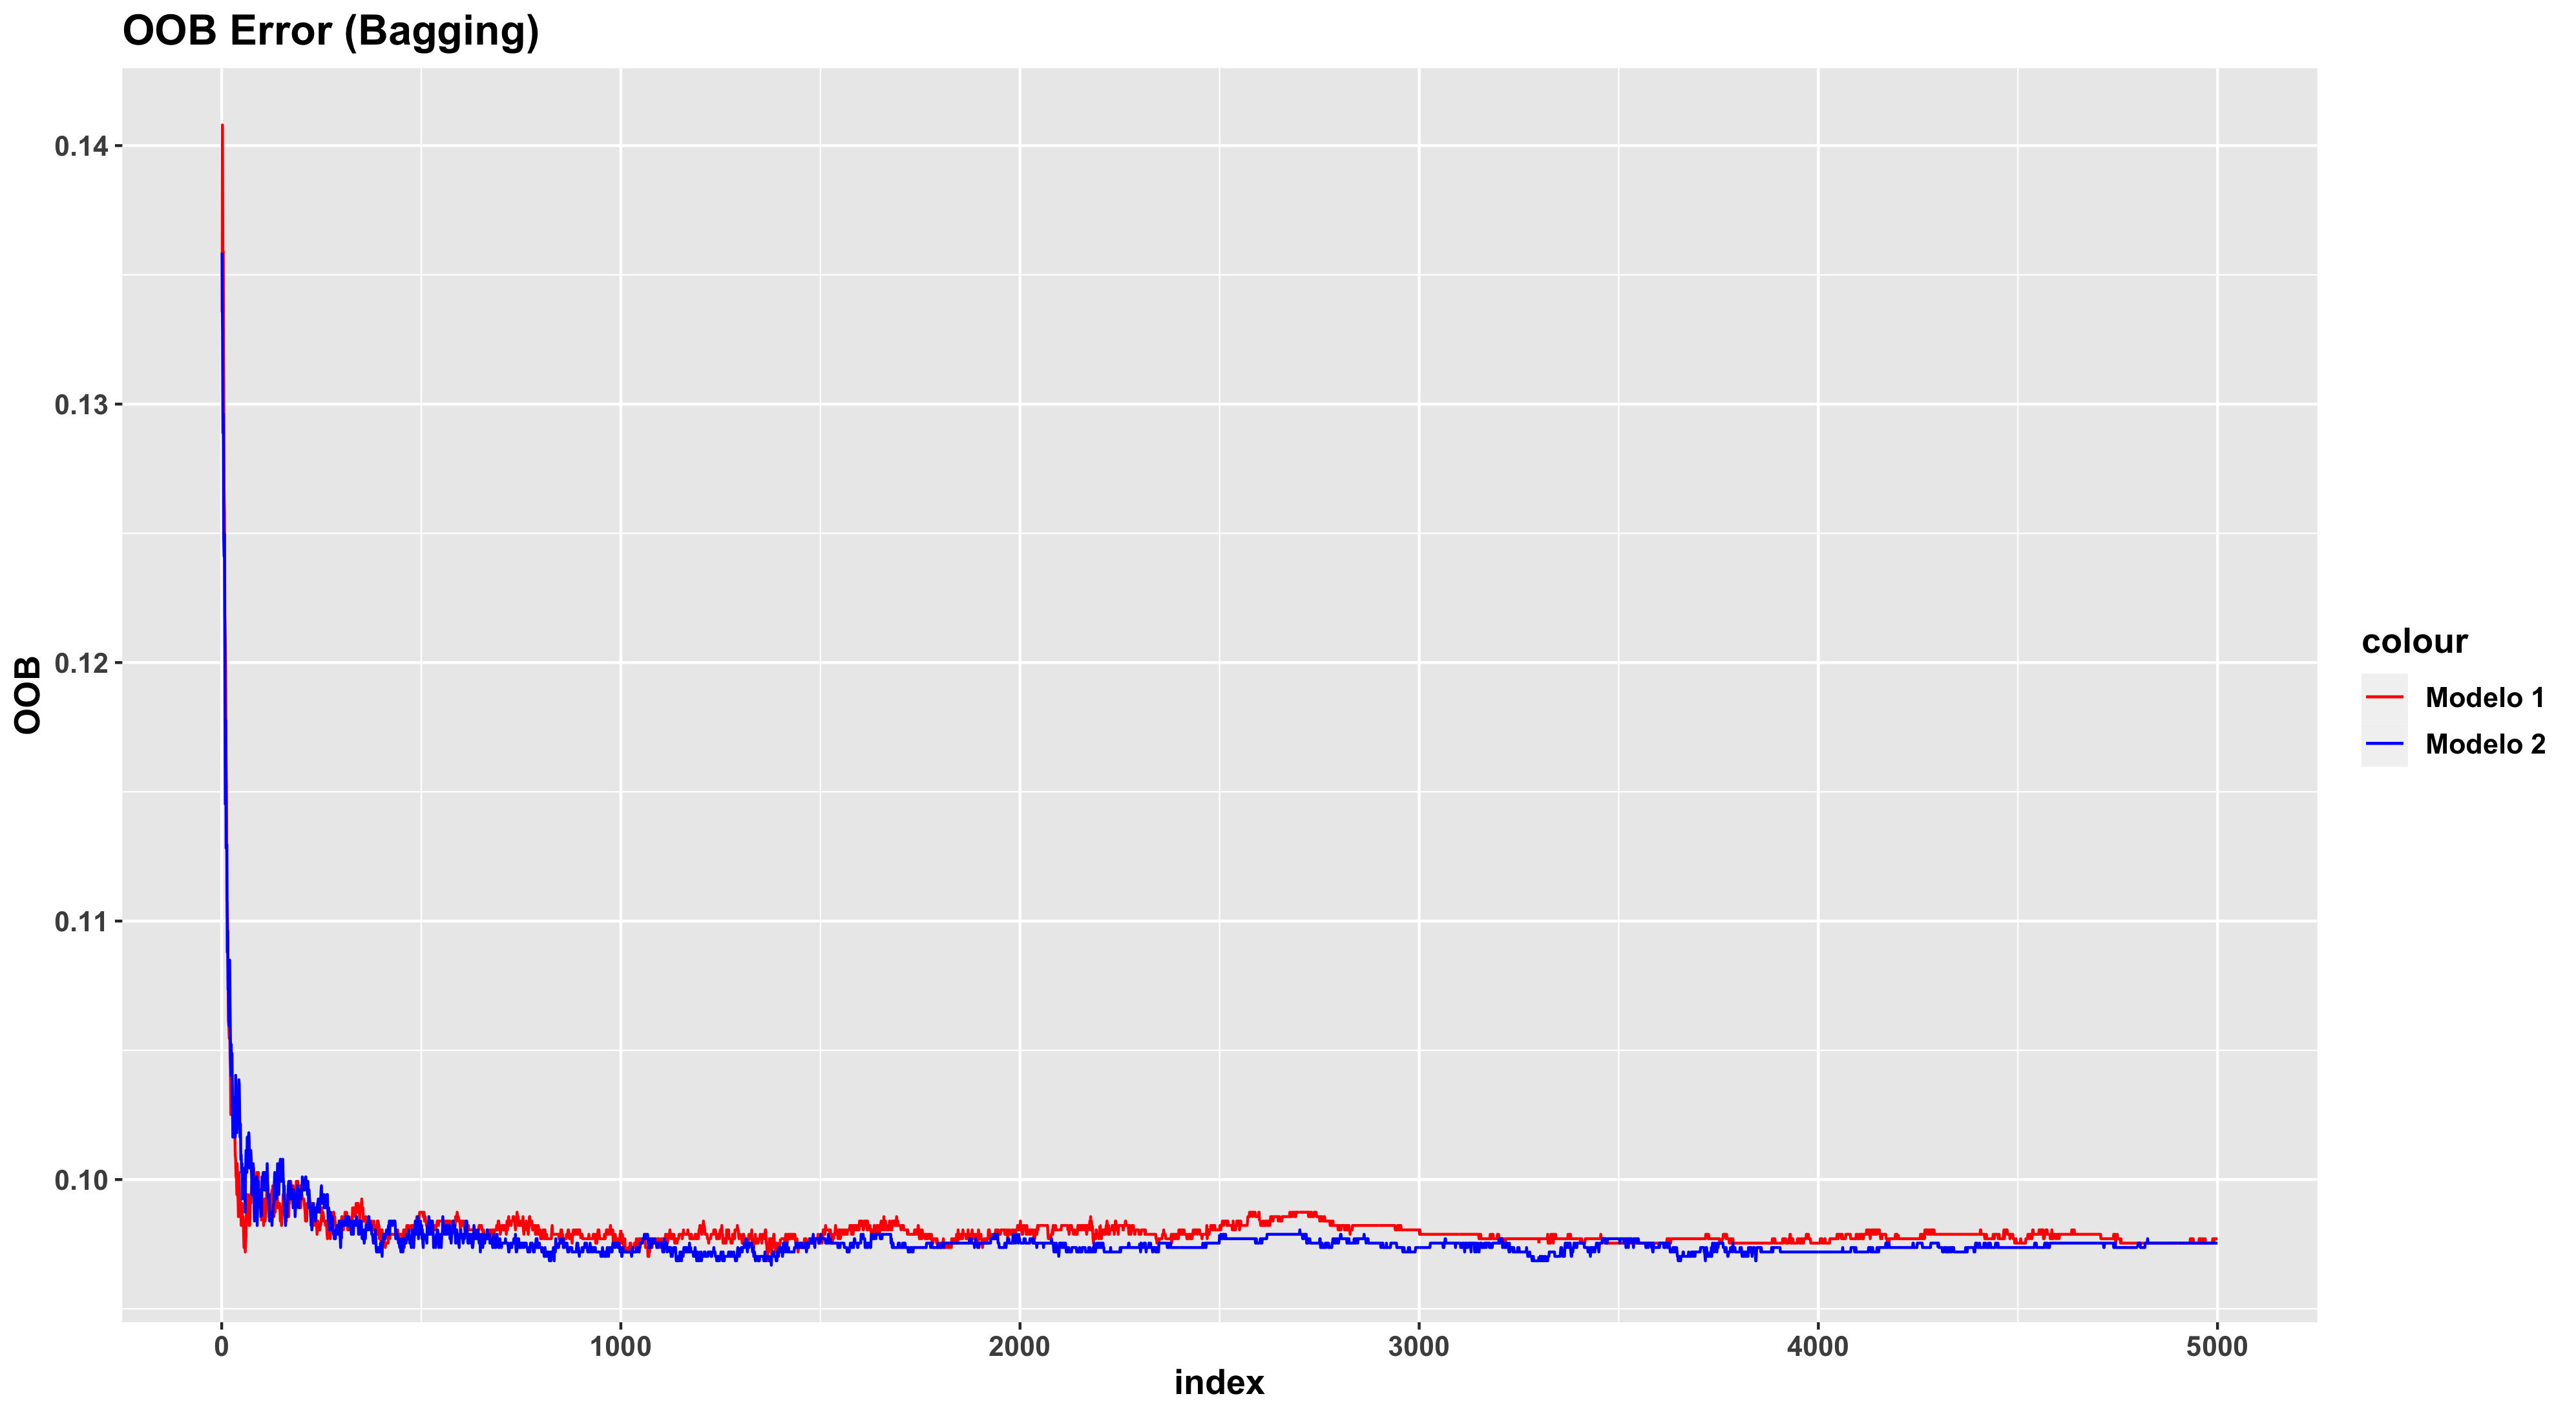
\includegraphics[width=0.99\linewidth,height=0.99\textheight,]{./charts/OOB_1} 

}

\caption{OOB Error (Modelos 1 y 2) (I)}\label{fig:unnamed-chunk-65}
\end{figure}

Analizando el error \emph{Out of bag}, \textbf{en ambos modelos el error
se estabiliza con aproximadamente 1000 árboles, obteniendo valores de
error inferiores a 0.1, similares a los obtenidos en los modelos de
red}. Si hacemos \emph{zoom} sobre el gráfico:

\begin{figure}[h!]

{\centering 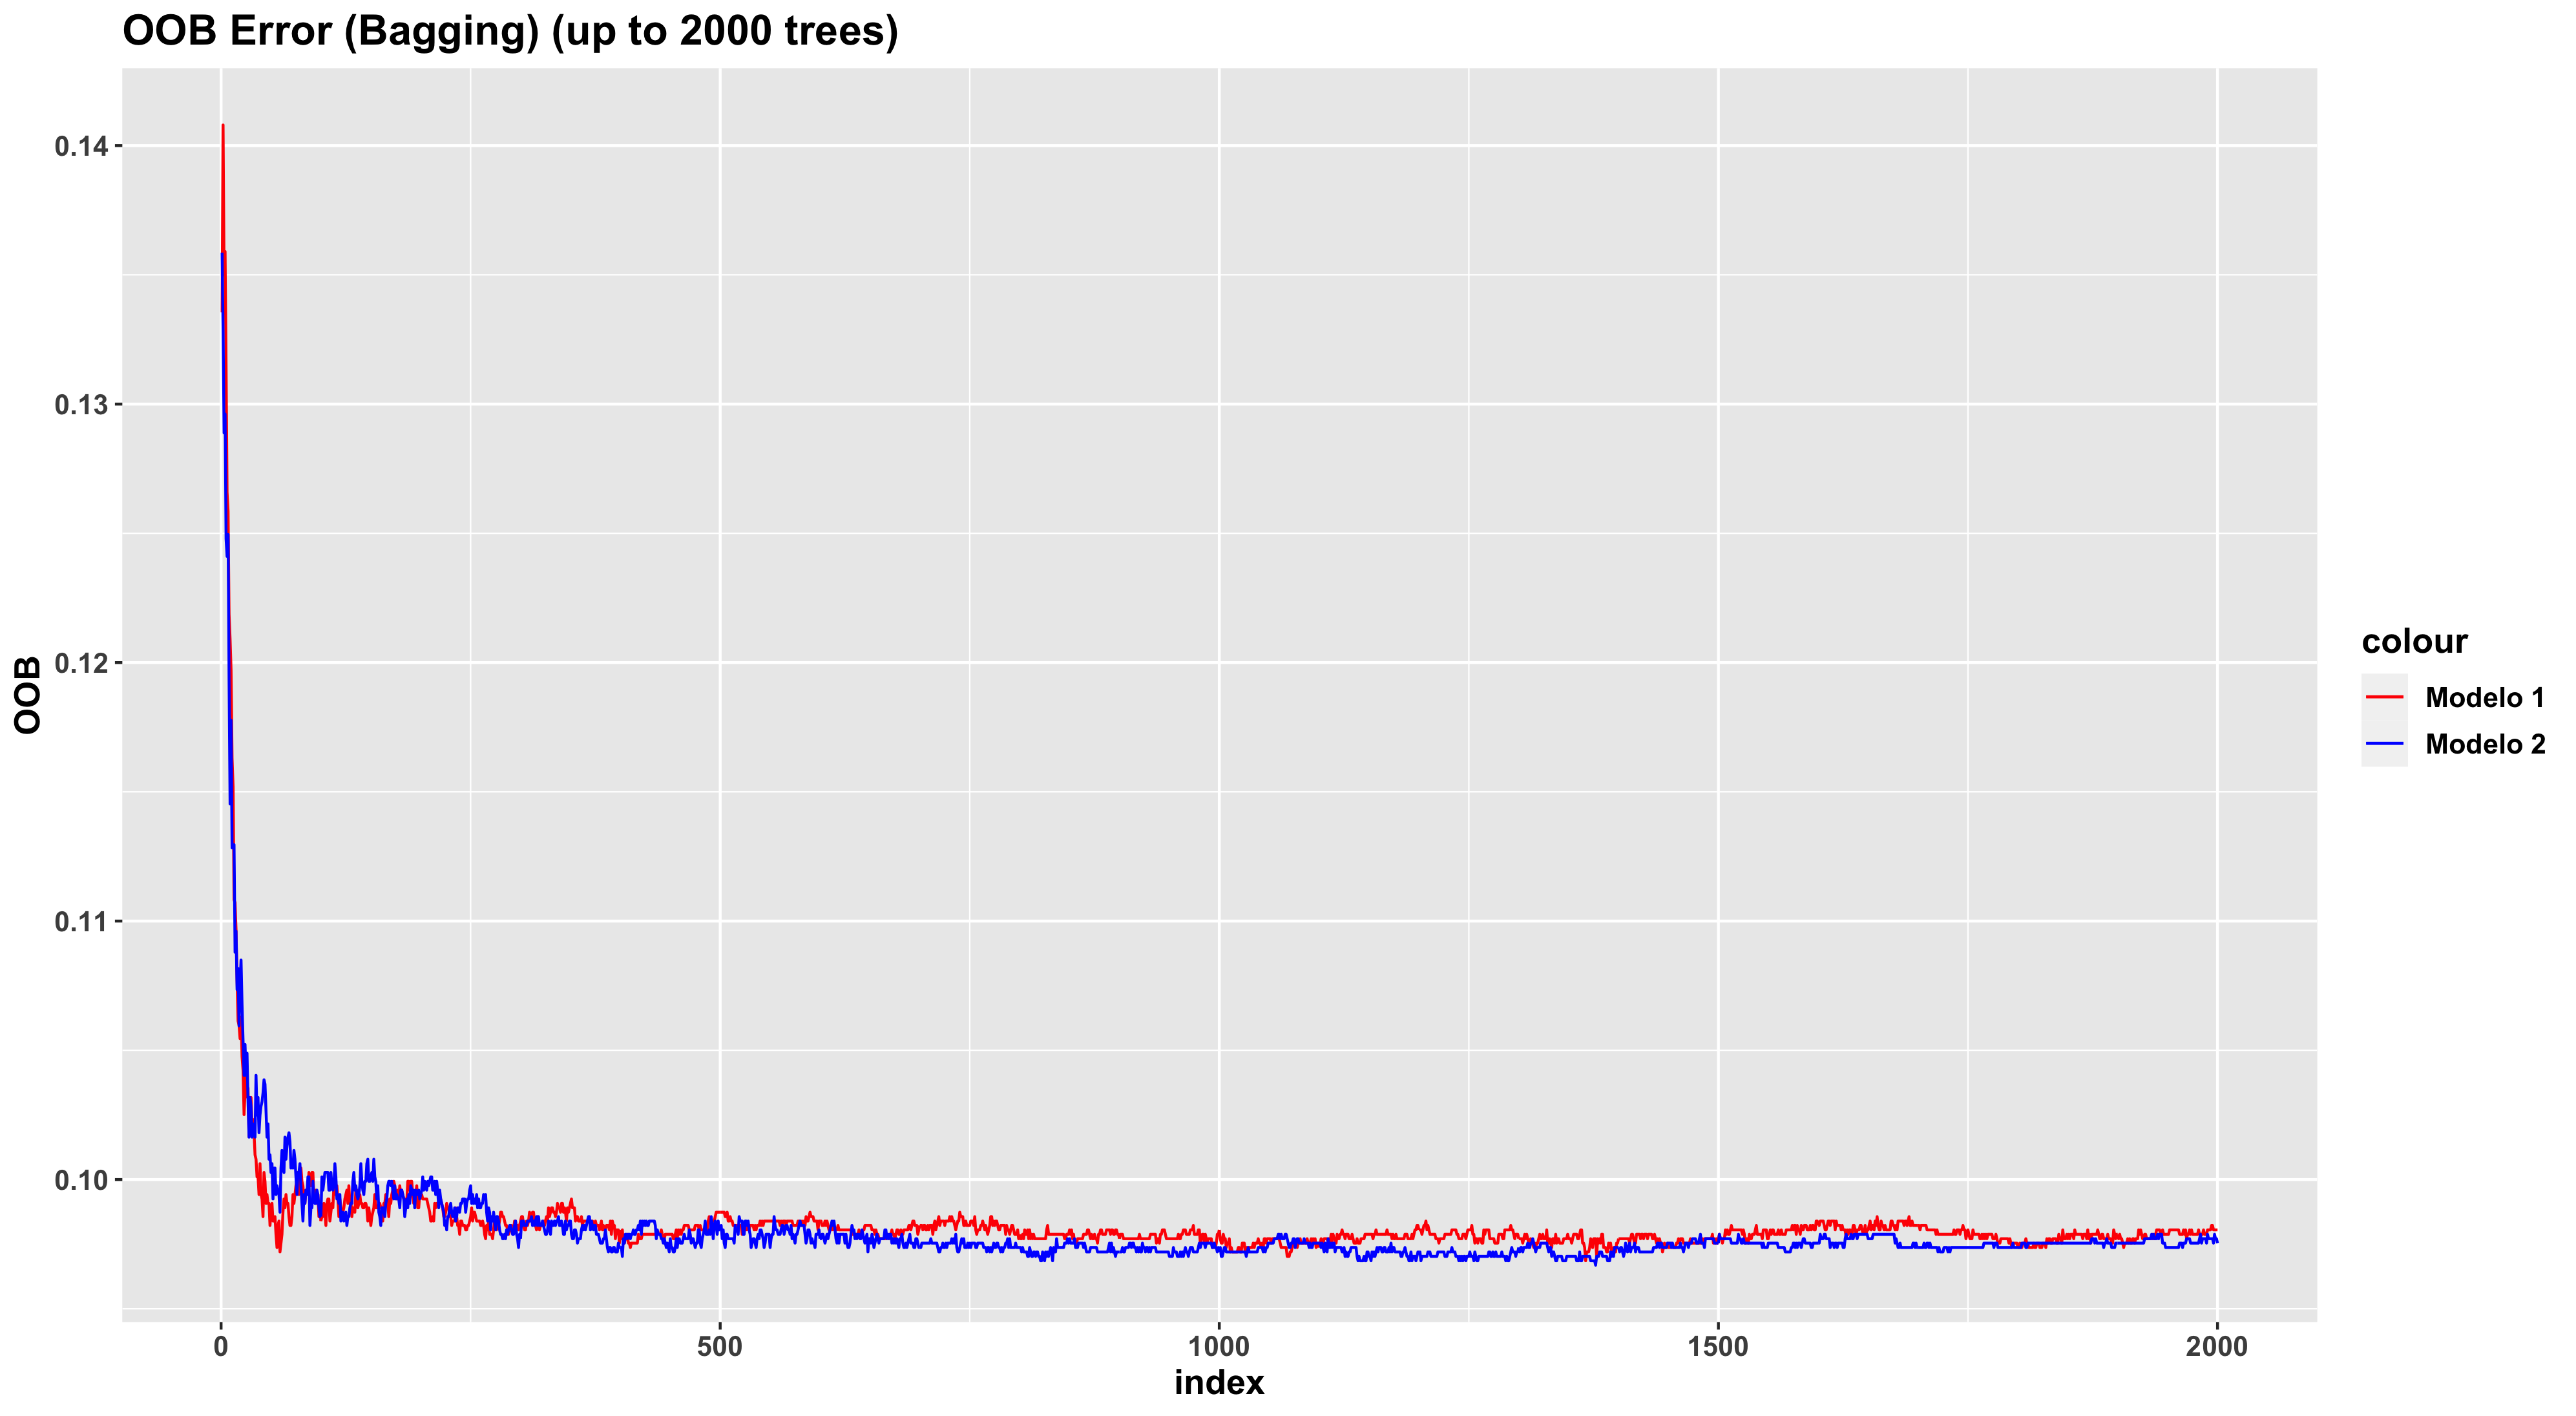
\includegraphics[width=0.99\linewidth,height=0.99\textheight,]{./charts/OOB_2} 

}

\caption{OOB Error (Modelos 1 y 2) (II)}\label{fig:unnamed-chunk-66}
\end{figure}

Observamos como a partir de 200-250 árboles, el error comienza a
situarse por debajo de 0.10. Sin embargo, \textbf{no es hasta los
900-1000 árboles cuando el error prácticamente se estabiliza, a partir
del cual se detectan ciertas fluctuaciones (subidas o bajadas en el
error), aunque de forma aleatoria}. Por tanto, \textbf{para ambos
modelos escogemos 900 como número de árboles}.

\begin{Shaded}
\begin{Highlighting}[]
\NormalTok{n.trees}\FloatTok{.1}\NormalTok{ <{-}}\StringTok{ }\DecValTok{900}\NormalTok{; n.trees}\FloatTok{.2}\NormalTok{ <{-}}\StringTok{ }\DecValTok{900}
\end{Highlighting}
\end{Shaded}

\hypertarget{modelo-1}{%
\subsection{7.2 Modelo 1}\label{modelo-1}}

En un primer comienzo, hagamos un repaso previo de los parámetros a
tunear en un modelo \emph{bagging}, junto con el número de árboles:

\emph{mtry}: número de variables sorteadas aleatoriamente en cada
división del árbol. Dado que se trata de un modelo \emph{bagging},
\textbf{establecemos en dicho parámetro el número total de variables
independientes del modelo}.

\emph{nodesize}: tamaño máximo de nodos finales.

\emph{sampsize}: número de observaciones seleccionadas aleatoriamente
(con o sin reemplazamiento) para la construcción del árbol.

\emph{replace}: si el sorteo anterior se realiza con o sin
reemplazamiento (por defecto, con reemplazamiento).

Dado que \emph{mtry} debe corresponder con el número de variables
\emph{input} y el número de árboles ya está definido, quedan por tunear
tanto \emph{nodesize} como \emph{sampsize} y \emph{replace}. Por tanto,
\textbf{comenzamos ajustando tanto el tamaño de la submuestra como el
tamaño máximo de nodos finales} (en el caso del parámetro
\emph{replace}, una vez obtenidos los modelos \emph{bagging} para ambos
\emph{sets}, con el mejor de ambos probaremos a seleccionar muestras sin
reemplazamiento).

Antes de tunear \emph{sampsize}, y dado que estamos trabajando con
validación cruzada, \textbf{dispondremos de menos observaciones para
construir el modelo, de forma que debemos establecer un tamaño máximo
sobre dicho parámetro}. Concretamente, dado que disponemos de 5854
observaciones y 5 grupos de validación cruzada, cada grupo tendrá
disponible 5854 * (4/5) \textasciitilde{} 4683 observaciones, siendo el
tamaño máximo de muestra que podemos probar:

\begin{Shaded}
\begin{Highlighting}[]
\NormalTok{mtry}\FloatTok{.1}\NormalTok{      <{-}}\StringTok{ }\DecValTok{5}
\CommentTok{\#{-}{-} Redondeamos 4683 a 4600}
\NormalTok{sampsizes}\FloatTok{.1}\NormalTok{ <{-}}\StringTok{ }\KeywordTok{list}\NormalTok{(}\DecValTok{1}\NormalTok{, }\DecValTok{100}\NormalTok{, }\DecValTok{500}\NormalTok{, }\DecValTok{1000}\NormalTok{, }\DecValTok{2000}\NormalTok{, }\DecValTok{3000}\NormalTok{, }\DecValTok{4600}\NormalTok{)}
\NormalTok{nodesizes}\FloatTok{.1}\NormalTok{ <{-}}\StringTok{ }\KeywordTok{list}\NormalTok{(}\DecValTok{5}\NormalTok{, }\DecValTok{10}\NormalTok{, }\DecValTok{20}\NormalTok{, }\DecValTok{30}\NormalTok{, }\DecValTok{40}\NormalTok{, }\DecValTok{50}\NormalTok{, }\DecValTok{100}\NormalTok{)}

\NormalTok{bagging\_modelo1 <{-}}\StringTok{ }\KeywordTok{tuneo\_bagging}\NormalTok{(surgical\_dataset, }\DataTypeTok{target =}\NormalTok{ target,}
                                 \DataTypeTok{lista.continua =}\NormalTok{ var\_modelo1,}
                                 \DataTypeTok{nodesizes =}\NormalTok{ nodesizes}\FloatTok{.1}\NormalTok{,}
                                 \DataTypeTok{sampsizes =}\NormalTok{ sampsizes}\FloatTok{.1}\NormalTok{, }\DataTypeTok{mtry =}\NormalTok{ mtry}\FloatTok{.1}\NormalTok{,}
                                 \DataTypeTok{ntree =}\NormalTok{ n.trees}\FloatTok{.1}\NormalTok{, }\DataTypeTok{grupos =} \DecValTok{5}\NormalTok{, }\DataTypeTok{repe =} \DecValTok{5}\NormalTok{)}
\end{Highlighting}
\end{Shaded}

A continuación, por cada combinación \emph{nodesize} - \emph{sampsize}
mostramos el promedio tanto de la tasa de fallos como de AUC:

\begin{figure}[h!]

{\centering 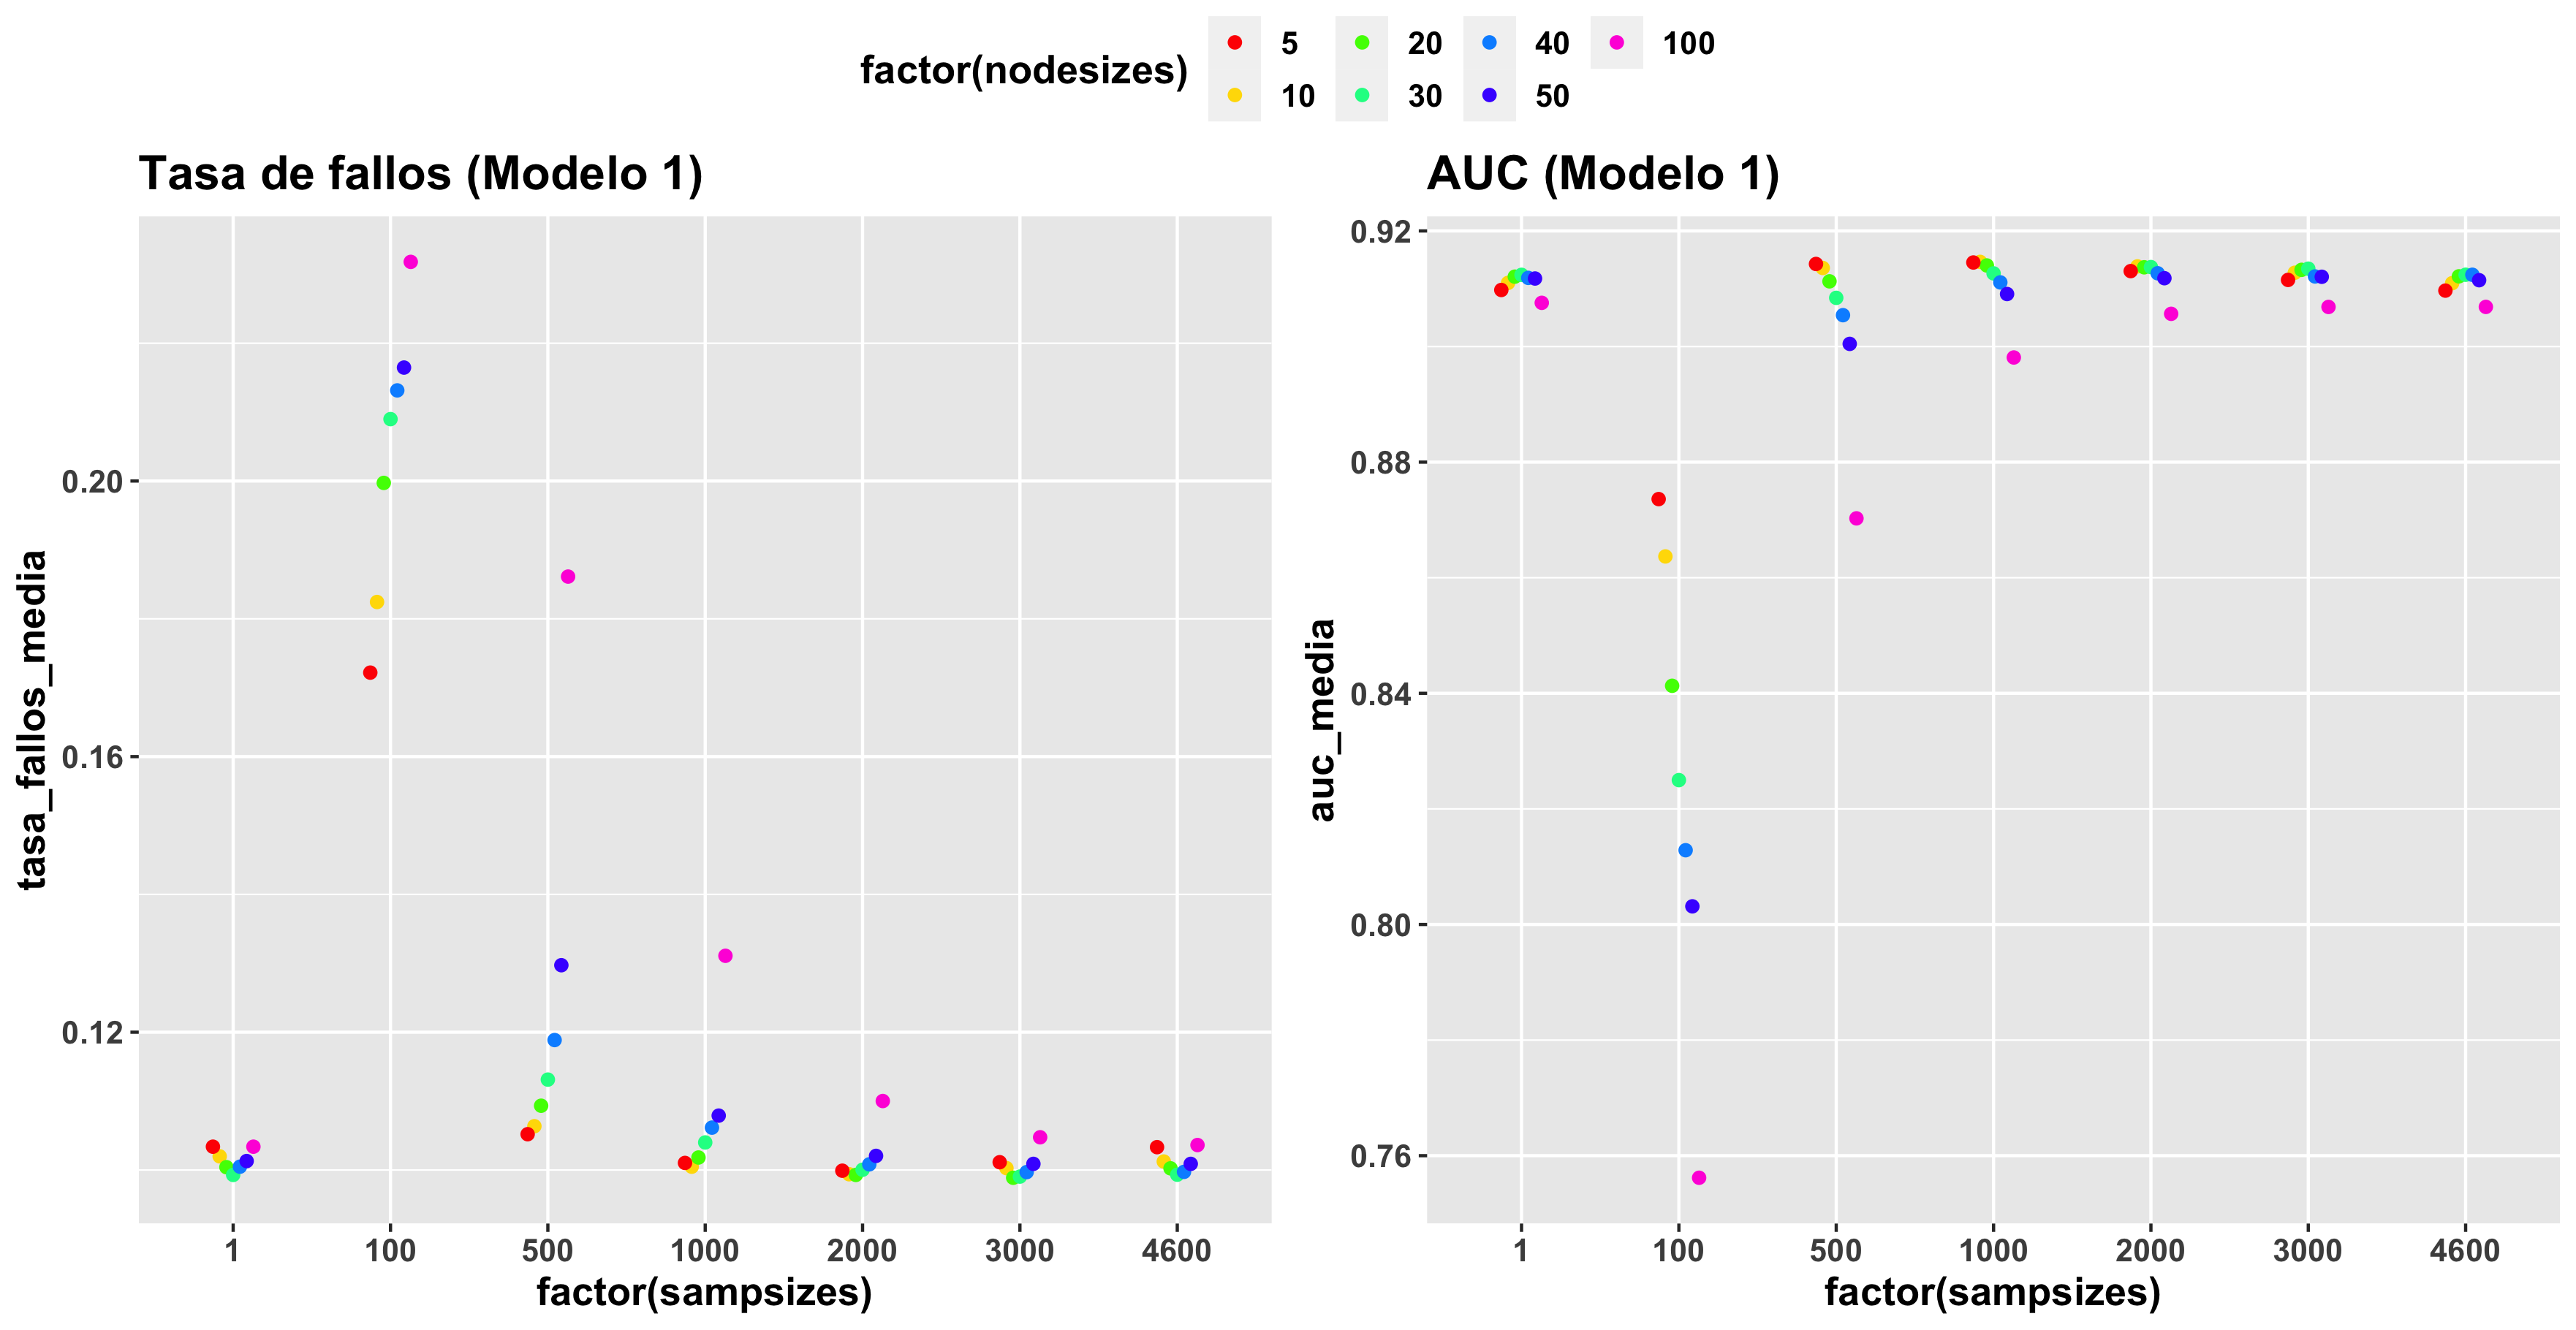
\includegraphics[width=0.99\linewidth,height=0.99\textheight,]{./charts/03_distribucion_auc_tasa_fallos_modelo1} 

}

\caption{Distribucion de la tasa de fallos y AUC por sampsize y nodesize (Modelo 1) (I)}\label{fig:unnamed-chunk-69}
\end{figure}

En un primer análisis, caben destacar fundamentalmente dos aspectos:

\begin{enumerate}
\def\labelenumi{\arabic{enumi}.}
\item
  En relación al \emph{nodesize}, tanto en tasa de fallos como en AUC,
  se obtienen buenos resultados en torno a un valor de 5-30,
  aproximadamente, pues a partir de 50-100 (árboles menos complejos), la
  precisión del modelo comienza a disminuir. Sin embargo, ¿Merece la
  pena aumentar la complejidad del árbol, disminuyendo el parámetro
  \emph{nodesize}? A simple vista, la diferencia entre un modelo de
  mayor complejidad ( \emph{nodesize} = 5 ), y un modelo de menor
  complejidad ( \emph{nodesize} = 20 ), es muy pequeña (punto rojo y
  verde). \textbf{Por tanto, una posibilidad sería decantarse por un
  \emph{nodesize} elevado, en torno a 20.}
\item
  Por otro lado, llama la atención el tuneo sobre el parámetro
  \emph{sampsize}. Bien es cierto que conforme aumenta el tamaño de la
  submuestra, mayor es la precisión. No obstante, ¿Qué diferencia existe
  entre un modelo en el que se utilizan todas las observaciones (
  \emph{sampsize} = 1 ) y un modelo con tan solo 500 o 1000 submuestras?
  No hay demasiada diferencia, en especial con un \emph{nodesize} en
  torno a 20, tal y como comentamos en el apartado anterior. De este
  modo, y gracias además al elevado número de árboles del que disponemos
  (900), \textbf{un valor \emph{sampsize} bajo permite no solo reducir
  el tiempo de cómputo para entrenar el modelo, sino además una mayor
  variedad en la construcción de cada uno de los árboles}.
\end{enumerate}

Es decir, para obtener un buen modelo \emph{bagging} \textbf{no es
necesario emplear todas las observaciones, ni tampoco árboles con
demasiada complejidad}, sino que con pocas muestras (en torno a 500), y
un \emph{nodesize} alto (en torno a 20), se obtienen muy buenos
resultados. Por tanto, una vez realizado el primer análisis, realizamos
una comparación (tanto del sesgo como de la varianza) sobre modelos
\emph{bagging} con un valor \emph{nodesize} pequeño (5), lo que se
traduce en árboles más complejos, frente a modelos con un valor alto (en
torno a 20). Del mismo modo, analizamos el sesgo y varianza con
diferentes valores de \emph{sampsize}, aumentando a 10 el número de
repeticiones para observar mejor su efecto:

\begin{Shaded}
\begin{Highlighting}[]
\NormalTok{nodesizes}\FloatTok{.1}\NormalTok{ <{-}}\StringTok{ }\KeywordTok{list}\NormalTok{(}\DecValTok{5}\NormalTok{, }\DecValTok{20}\NormalTok{)}
\CommentTok{\#{-}{-} Probamos con un sampsize entre 500 y 2000 observaciones (1 = todas las observaciones)}
\NormalTok{sampsizes}\FloatTok{.1}\NormalTok{ <{-}}\StringTok{ }\KeywordTok{list}\NormalTok{(}\DecValTok{1}\NormalTok{, }\DecValTok{500}\NormalTok{, }\DecValTok{1000}\NormalTok{, }\DecValTok{1500}\NormalTok{, }\DecValTok{2000}\NormalTok{)}
\NormalTok{bagging\_modelo1\_v2 <{-}}\StringTok{ }\KeywordTok{tuneo\_bagging}\NormalTok{(surgical\_dataset, }\DataTypeTok{target =}\NormalTok{ target,}
                                    \DataTypeTok{lista.continua =}\NormalTok{ var\_modelo1,}
                                    \DataTypeTok{nodesizes =}\NormalTok{ nodesizes}\FloatTok{.1}\NormalTok{,}
                                    \DataTypeTok{sampsizes =}\NormalTok{ sampsizes}\FloatTok{.1}\NormalTok{, }\DataTypeTok{mtry =}\NormalTok{ mtry}\FloatTok{.1}\NormalTok{,}
                                    \DataTypeTok{ntree =}\NormalTok{ n.trees}\FloatTok{.1}\NormalTok{, }\DataTypeTok{grupos =} \DecValTok{5}\NormalTok{, }\DataTypeTok{repe =} \DecValTok{10}\NormalTok{,}
                                    \DataTypeTok{show\_nrnodes =} \StringTok{"yes"}\NormalTok{)}
\end{Highlighting}
\end{Shaded}

\begin{figure}[h!]

{\centering 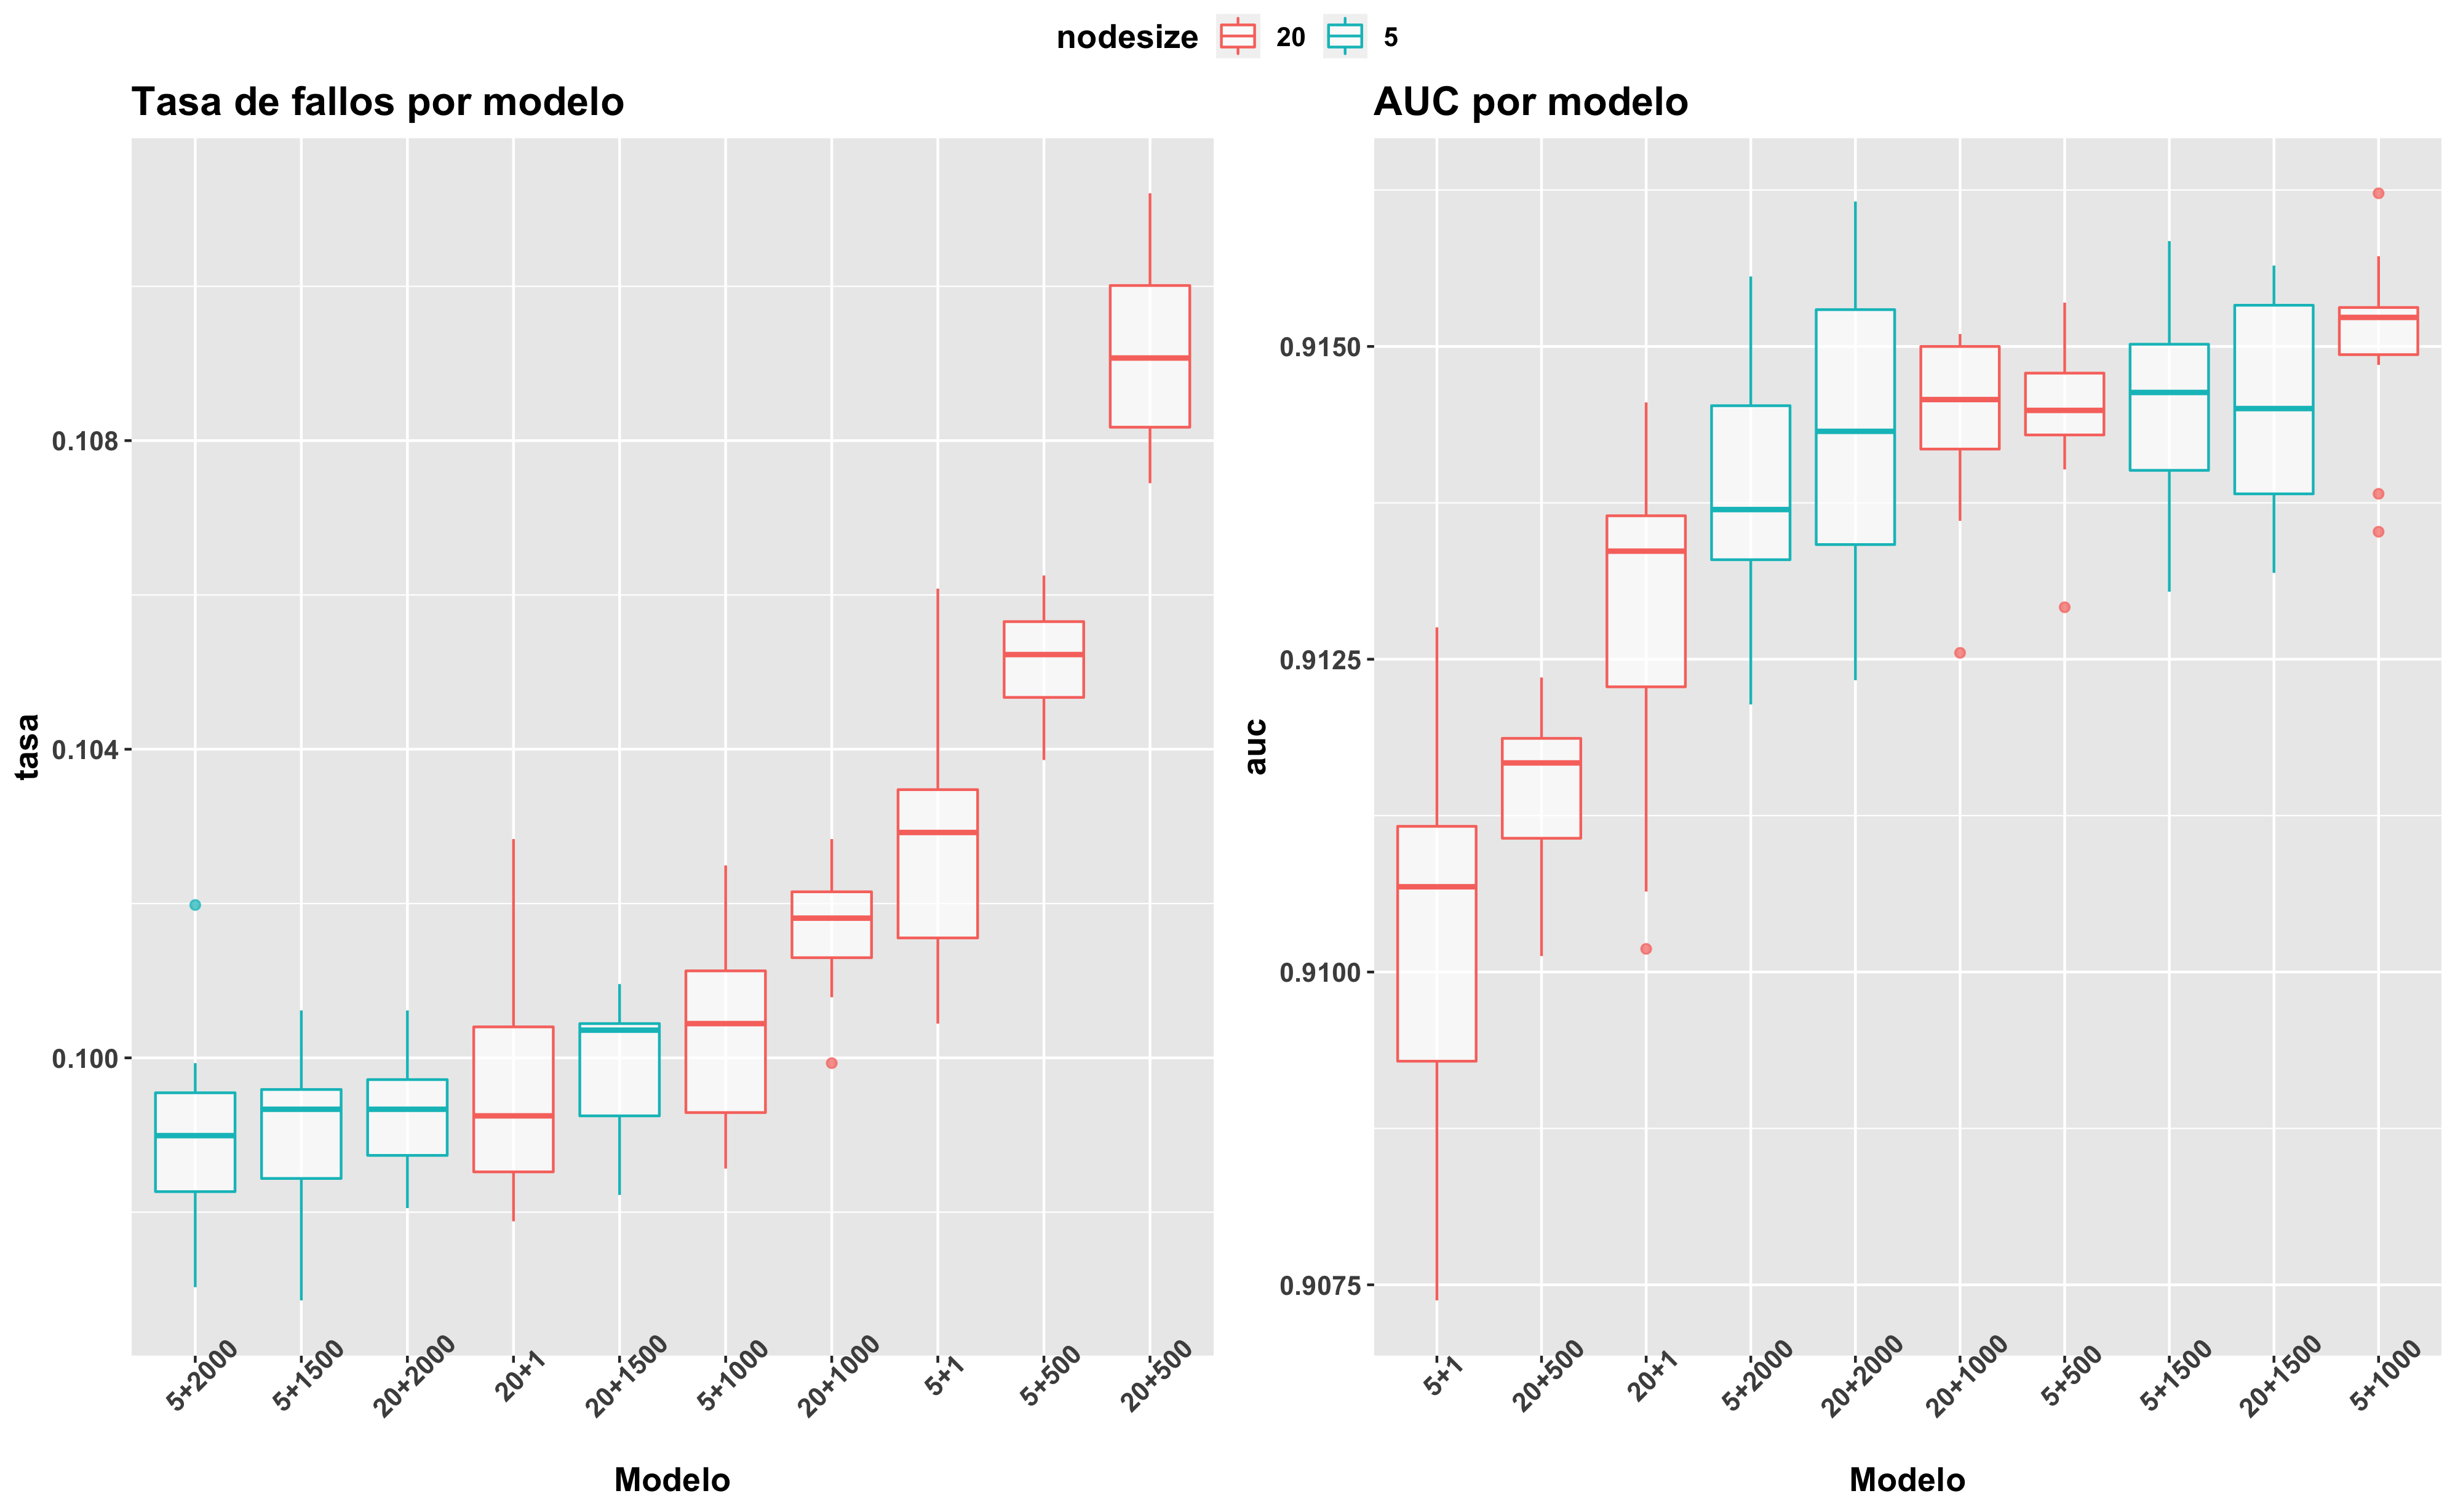
\includegraphics[width=0.99\linewidth,height=0.99\textheight,]{./charts/03_distribucion_auc_tasa_fallos_modelo1_comp} 

}

\caption{Distribucion de la tasa de fallos y AUC por sampsize y nodesize (Modelo 1) (II)}\label{fig:unnamed-chunk-71}
\end{figure}

Nuevamente, sin fijarnos en la escala del eje, una posible opción a
decantarse sería elegir un modelo con \emph{nodesize} 5 y
\emph{sampsize} 1000, pues presenta el mayor valor AUC y una tasa de
fallos baja. No obstante, los valores del eje pueden llevarnos a engaño.
Por ejemplo, la diferencia entre este modelo y uno mucho más sencillo
como es el caso de \emph{nodesize} 20 y \emph{sampsize} en torno a
500-1000 (20 + 500 o 20 + 1000) es muy pequeña (hablamos de una tasa de
fallos en torno a 0.10 y un AUC de 0.91, por lo que la diferencia es del
órden de milésimas), incluso con un menor número de muestras la varianza
de los modelos se ve reducida en comparación con usar todas las
observaciones, aunque la diferencia (por las escalas del eje) sea menor.

Sin embargo, ¿Y si aumentamos \emph{nodesize} a 50?

\begin{figure}[h!]

{\centering 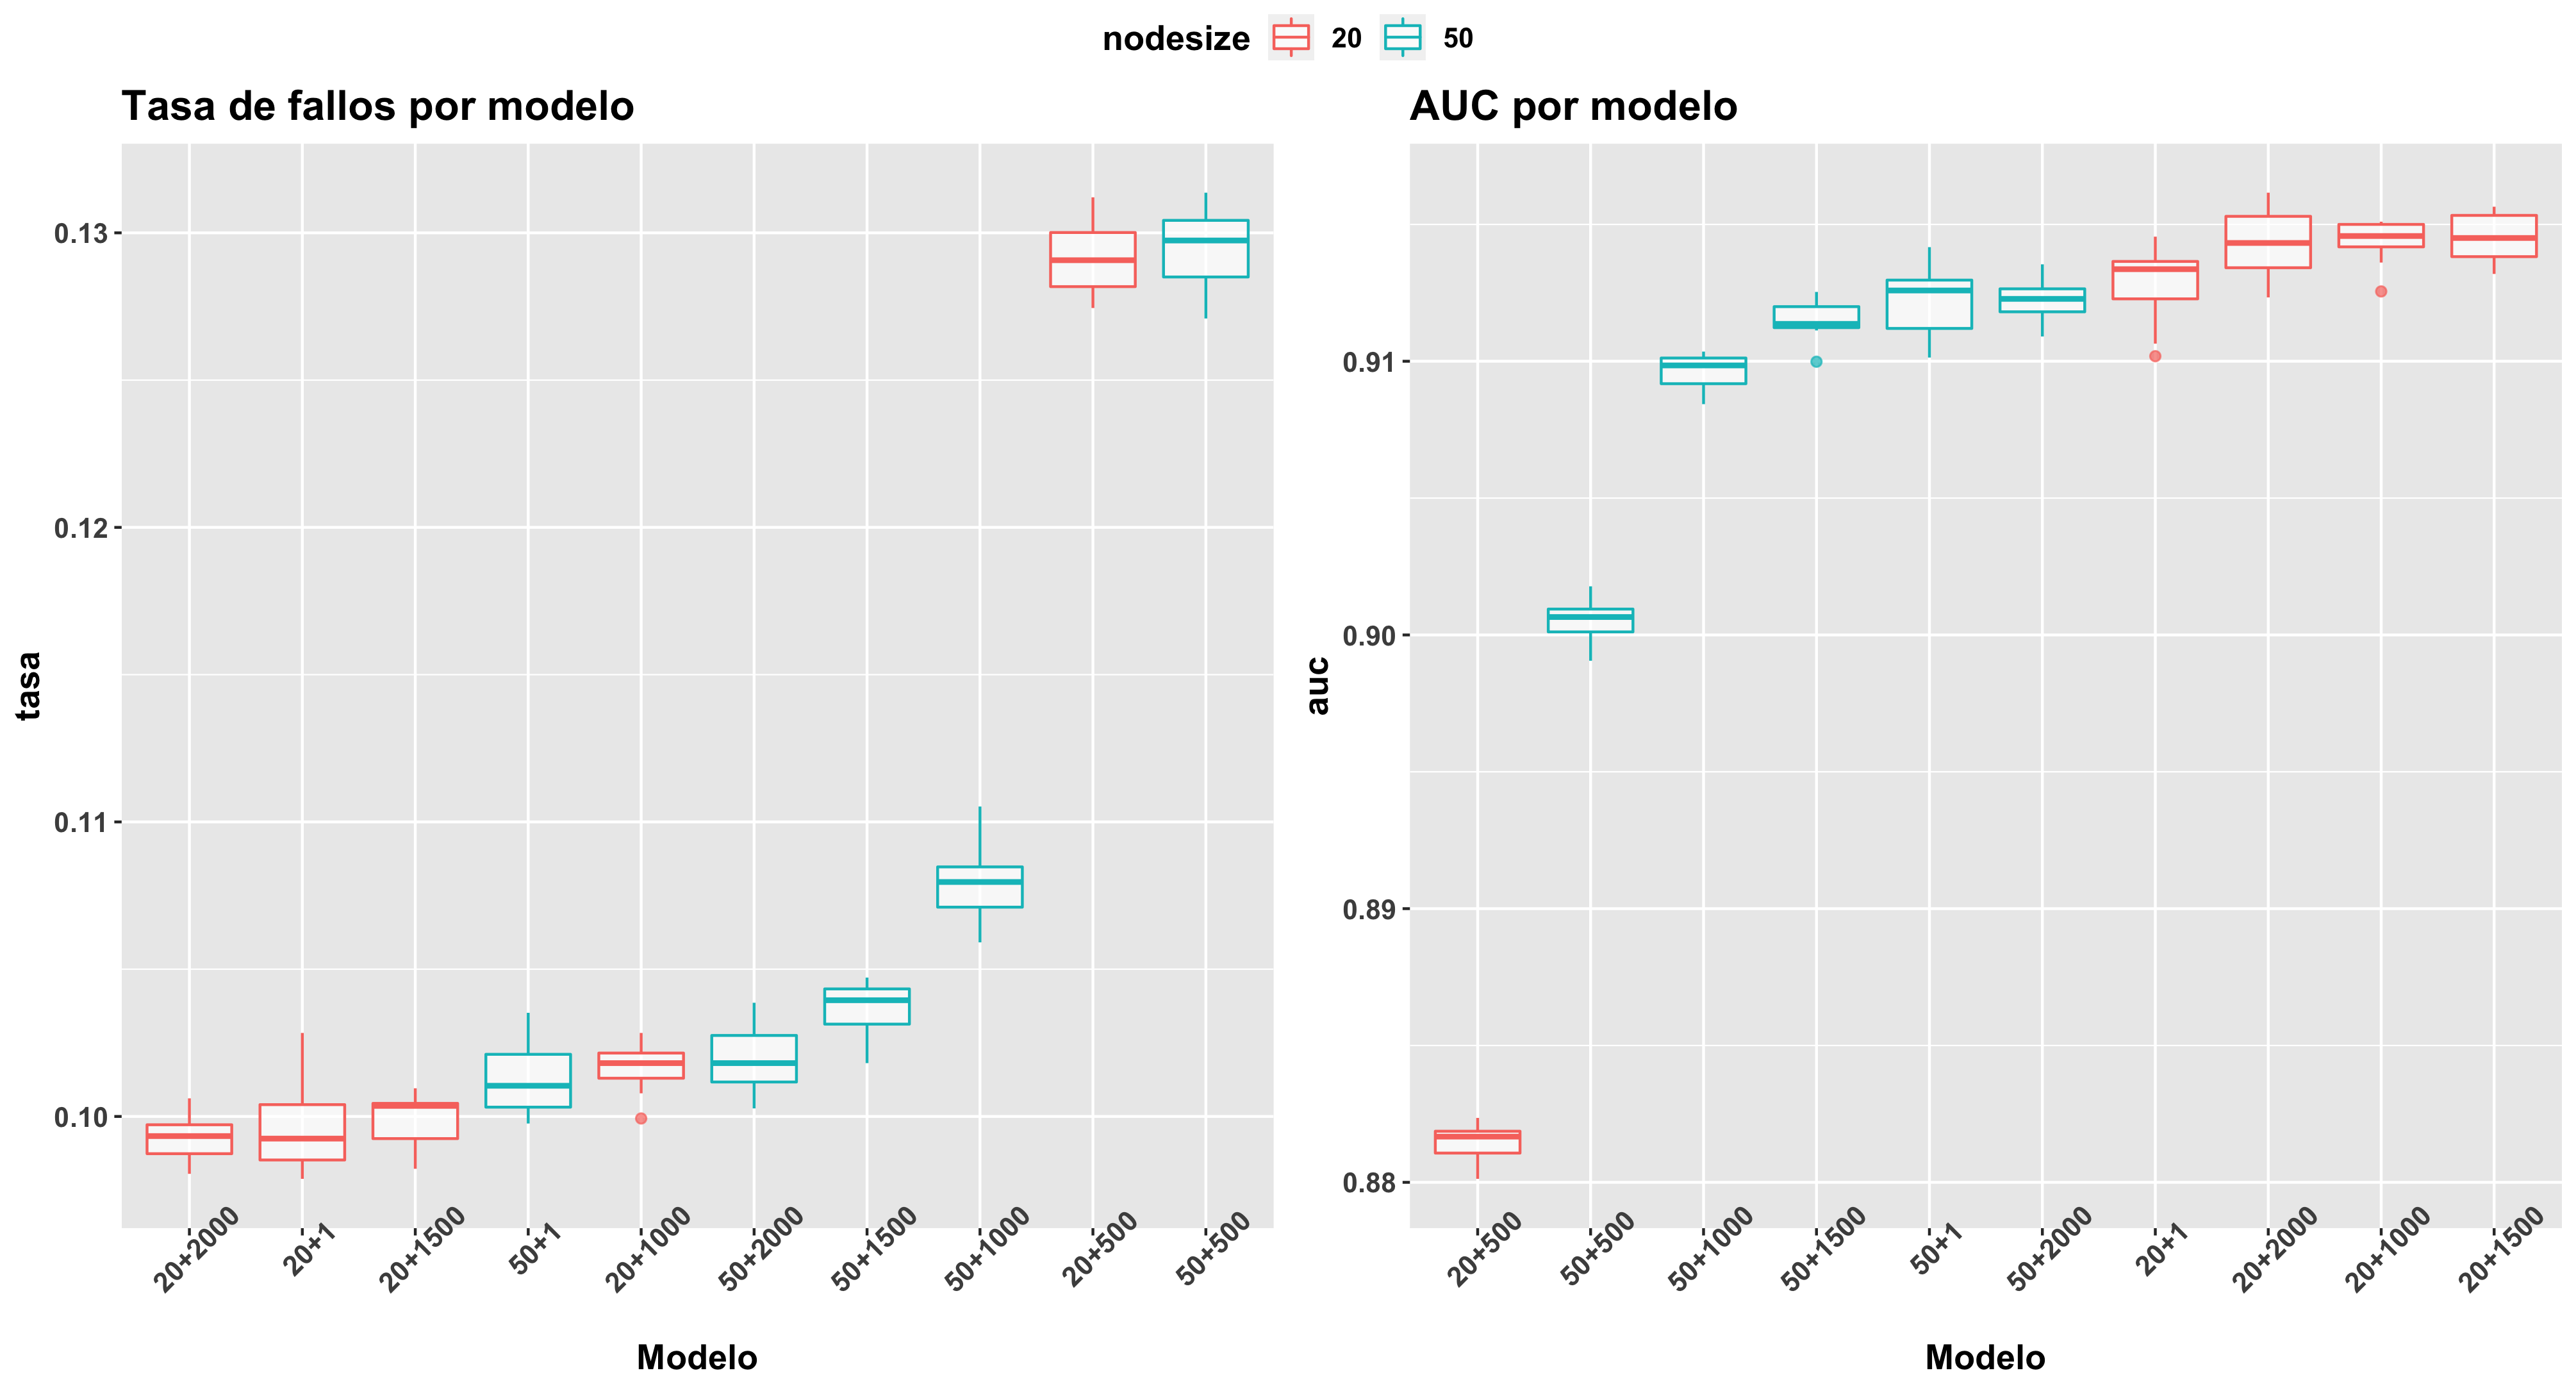
\includegraphics[width=0.99\linewidth,height=0.99\textheight,]{./charts/03_distribucion_auc_tasa_fallos_modelo1_comp_50rep} 

}

\caption{Distribucion de la tasa de fallos y AUC por sampsize y nodesize (Modelo 1) (III)}\label{fig:unnamed-chunk-72}
\end{figure}

A simple vista, \textbf{los resultados obtenidos son muy similares en
ambos casos}, especialmente en \emph{AUC}, donde la diferencia entre el
mejor modelo (20 + 1500) y el peor (50 + 500) es de tan solo 0.01. Sin
embargo, y en relación con la tasa de fallos, para alcanzar un valor en
torno al 10 \% con un \emph{nodesize} = 50, se requiere por lo general
un mayor tamaño de submuestra, dado que la complejidad del árbol es
menor. Sin embargo, con un valor \emph{nodesize} menor (20), se
requieren menos observaciones.

Por tanto, dada la poca ganancia que presentan los modelos complejos,
\textbf{nos decantamos por un modelo \emph{bagging} con \emph{nodesize}
= 20 y un tamaño de muestra en torno a 500 y 1000}. Sobre ambos
candidatos, para controlar mejor el tamaño óptimo de la muestra,
probamos con una validación cruzada de 10 grupos y 20 repeticiones:

\begin{figure}[h!]

{\centering 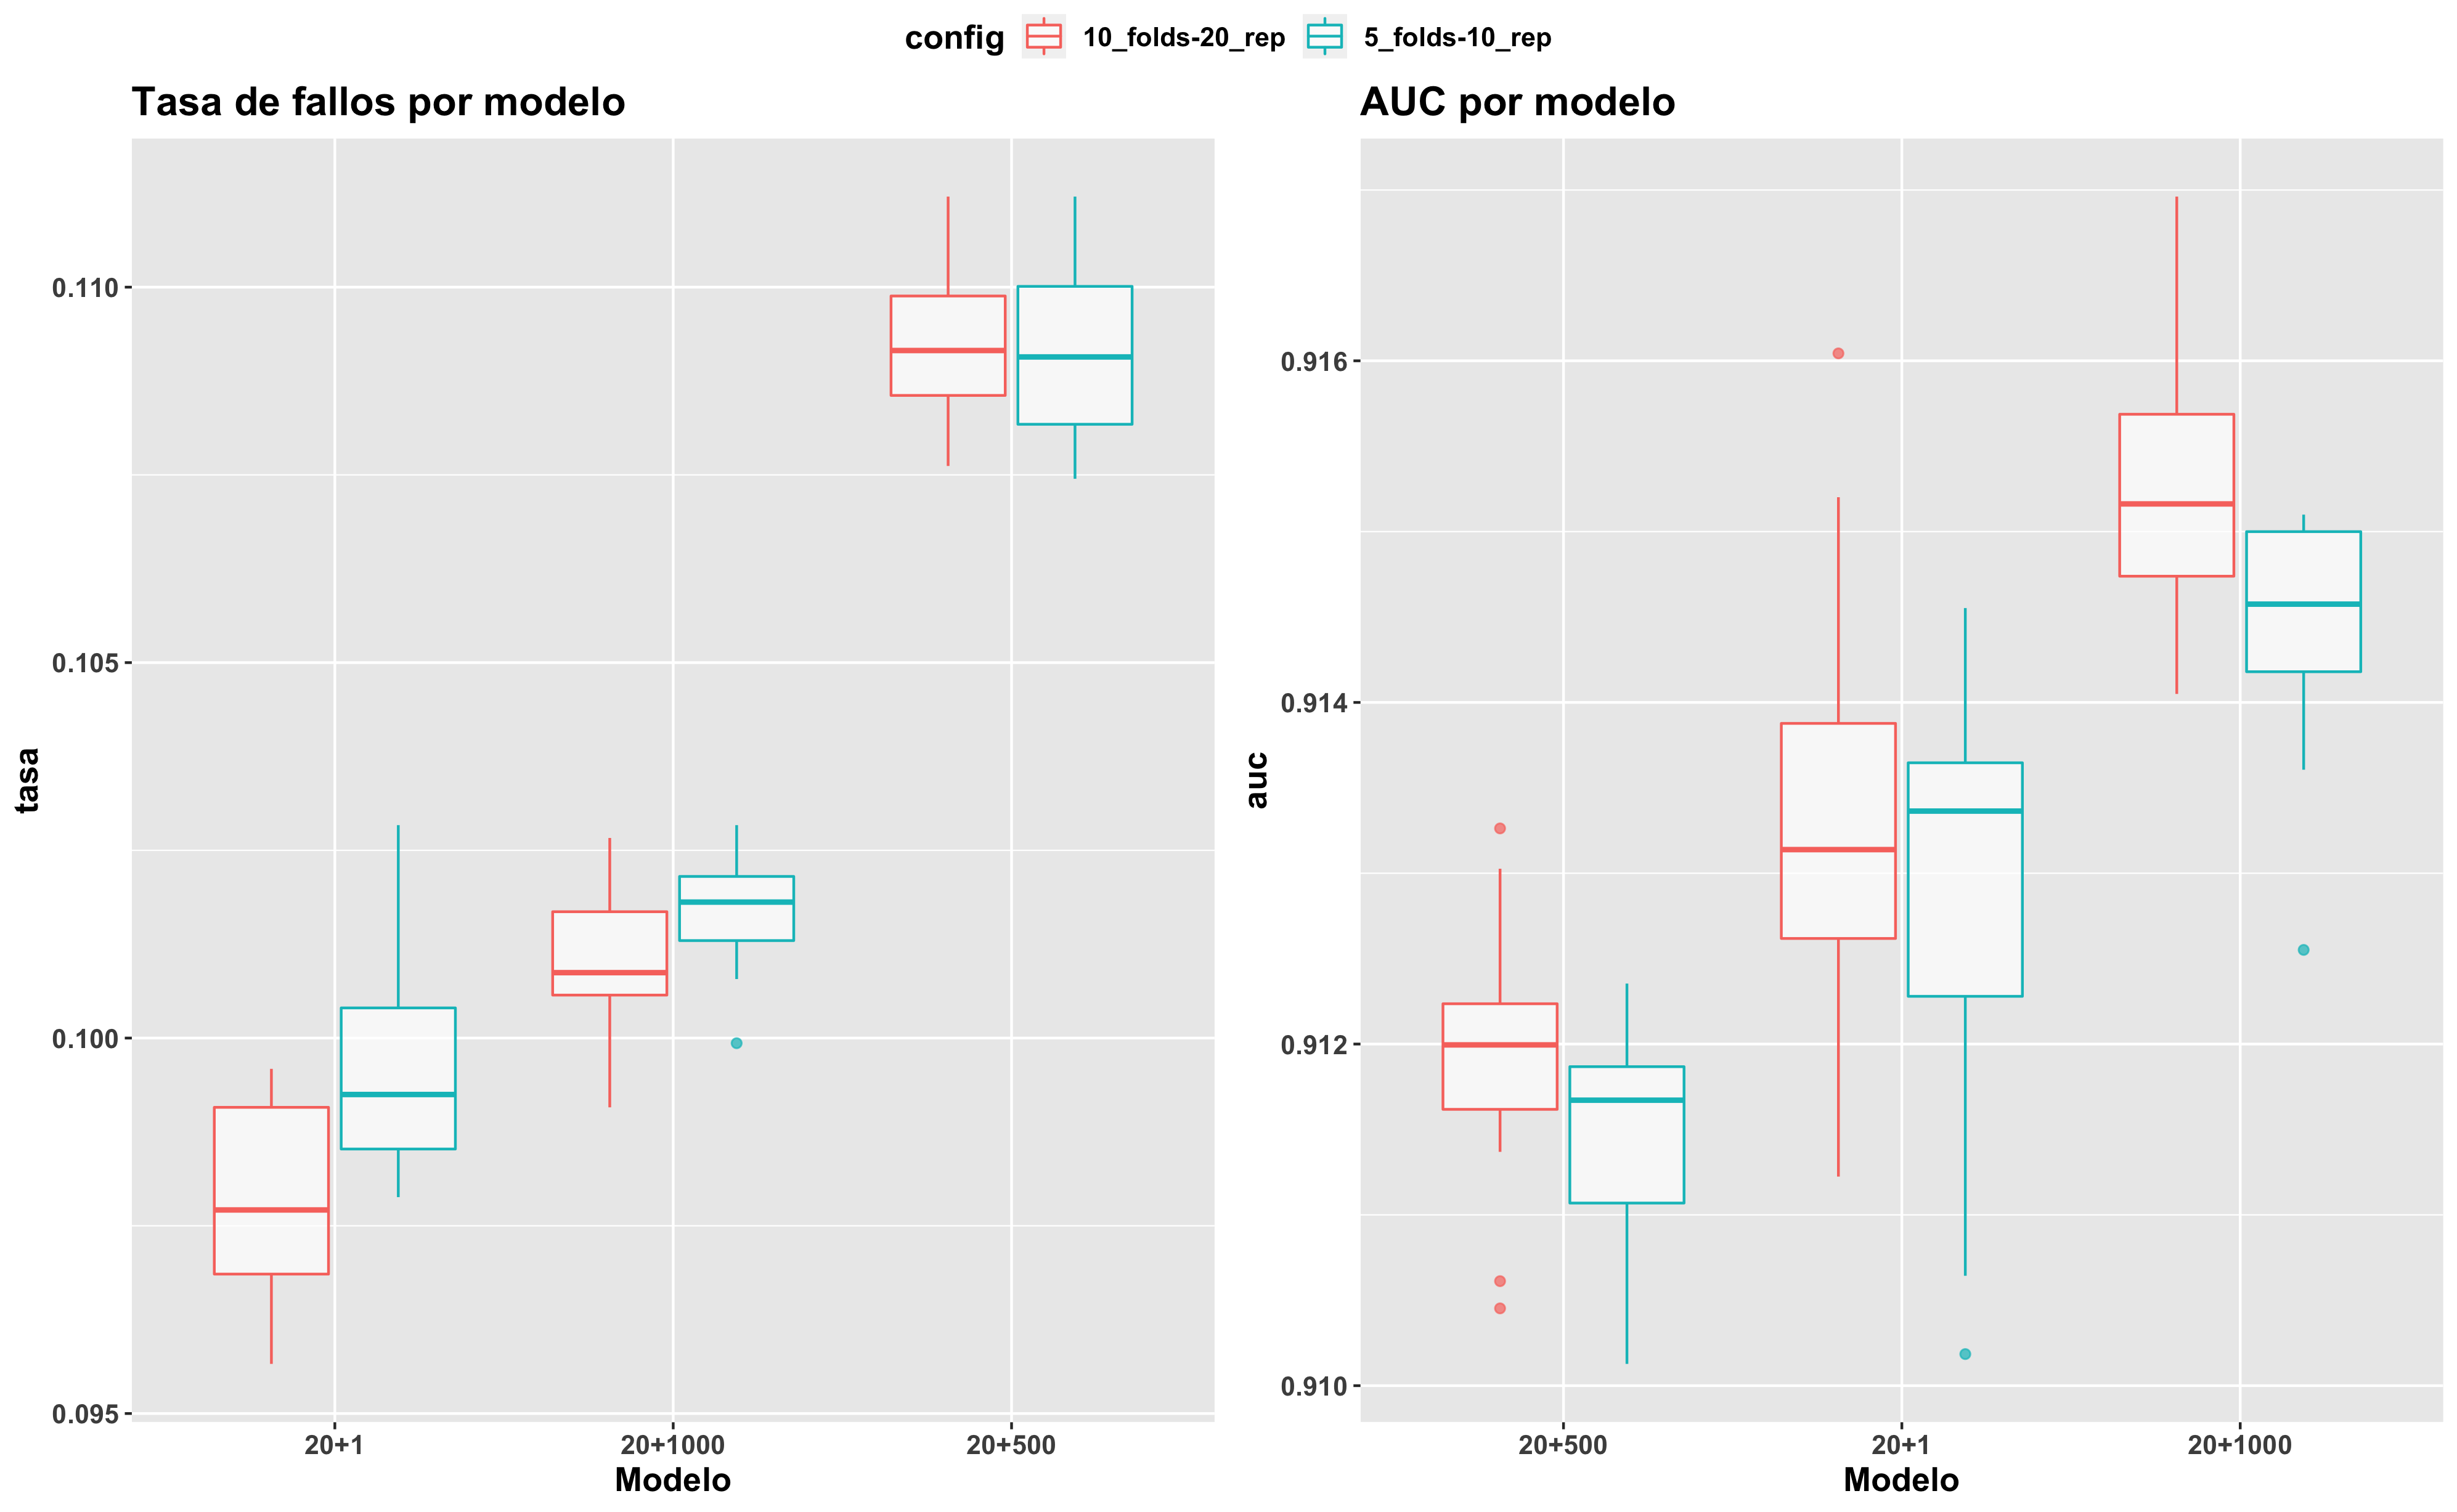
\includegraphics[width=0.99\linewidth,height=0.99\textheight,]{./charts/bagging/bis_03_comparacion_final_modelo1_5_10_folds} 

}

\caption{Distribucion de la tasa de fallos y AUC (Modelo 1) aumentando grupos y repeticiones}\label{fig:unnamed-chunk-73}
\end{figure}

Por lo general, incluso aumentando el número de grupos y repeticiones,
el orden de los modelos se mantiene idéntico, tanto en tasa de fallos
como en AUC. Por tanto, de los dos posibles modelos candidatos (con
\emph{sampsize} 500 o 1000), aunque la diferencia entre ambos, así como
el sesgo y varianza no sean muy significativas (dada la escala de los
ejes), \textbf{nos decantamos por un modelo con un tamaño de 1000
submuestras}, es decir, con tan solo el 1000 / 5854 \textasciitilde{} 17
\% de las observaciones.

\hypertarget{modelo-2}{%
\subsection{7.3 Modelo 2}\label{modelo-2}}

Del mismo modo, realizamos los mismos pasos con el segundo \emph{set} de
cuatro variables, comenzando con el tuneo tanto de \emph{nodesize} como
de \emph{sampsize}, obteniendo el promedio en tasa de fallos y AUC con 5
repeticiones:

\begin{Shaded}
\begin{Highlighting}[]
\NormalTok{mtry}\FloatTok{.2}\NormalTok{      <{-}}\StringTok{ }\DecValTok{4}
\NormalTok{sampsizes}\FloatTok{.2}\NormalTok{ <{-}}\StringTok{ }\KeywordTok{list}\NormalTok{(}\DecValTok{1}\NormalTok{, }\DecValTok{100}\NormalTok{, }\DecValTok{500}\NormalTok{, }\DecValTok{1000}\NormalTok{, }\DecValTok{2000}\NormalTok{, }\DecValTok{3000}\NormalTok{, }\DecValTok{4600}\NormalTok{)}
\NormalTok{nodesizes}\FloatTok{.2}\NormalTok{ <{-}}\StringTok{ }\KeywordTok{list}\NormalTok{(}\DecValTok{5}\NormalTok{, }\DecValTok{10}\NormalTok{, }\DecValTok{20}\NormalTok{, }\DecValTok{30}\NormalTok{, }\DecValTok{40}\NormalTok{, }\DecValTok{50}\NormalTok{, }\DecValTok{100}\NormalTok{)}

\NormalTok{bagging\_modelo1 <{-}}\StringTok{ }\KeywordTok{tuneo\_bagging}\NormalTok{(surgical\_dataset, }\DataTypeTok{target =}\NormalTok{ target,}
                                 \DataTypeTok{lista.continua =}\NormalTok{ var\_modelo2,}
                                 \DataTypeTok{nodesizes =}\NormalTok{ nodesizes}\FloatTok{.2}\NormalTok{,}
                                 \DataTypeTok{sampsizes =}\NormalTok{ sampsizes}\FloatTok{.2}\NormalTok{, }\DataTypeTok{mtry =}\NormalTok{ mtry}\FloatTok{.2}\NormalTok{,}
                                 \DataTypeTok{ntree =}\NormalTok{ n.trees}\FloatTok{.2}\NormalTok{, }\DataTypeTok{grupos =} \DecValTok{5}\NormalTok{, }\DataTypeTok{repe =} \DecValTok{5}\NormalTok{)}
\end{Highlighting}
\end{Shaded}

\begin{figure}[h!]

{\centering 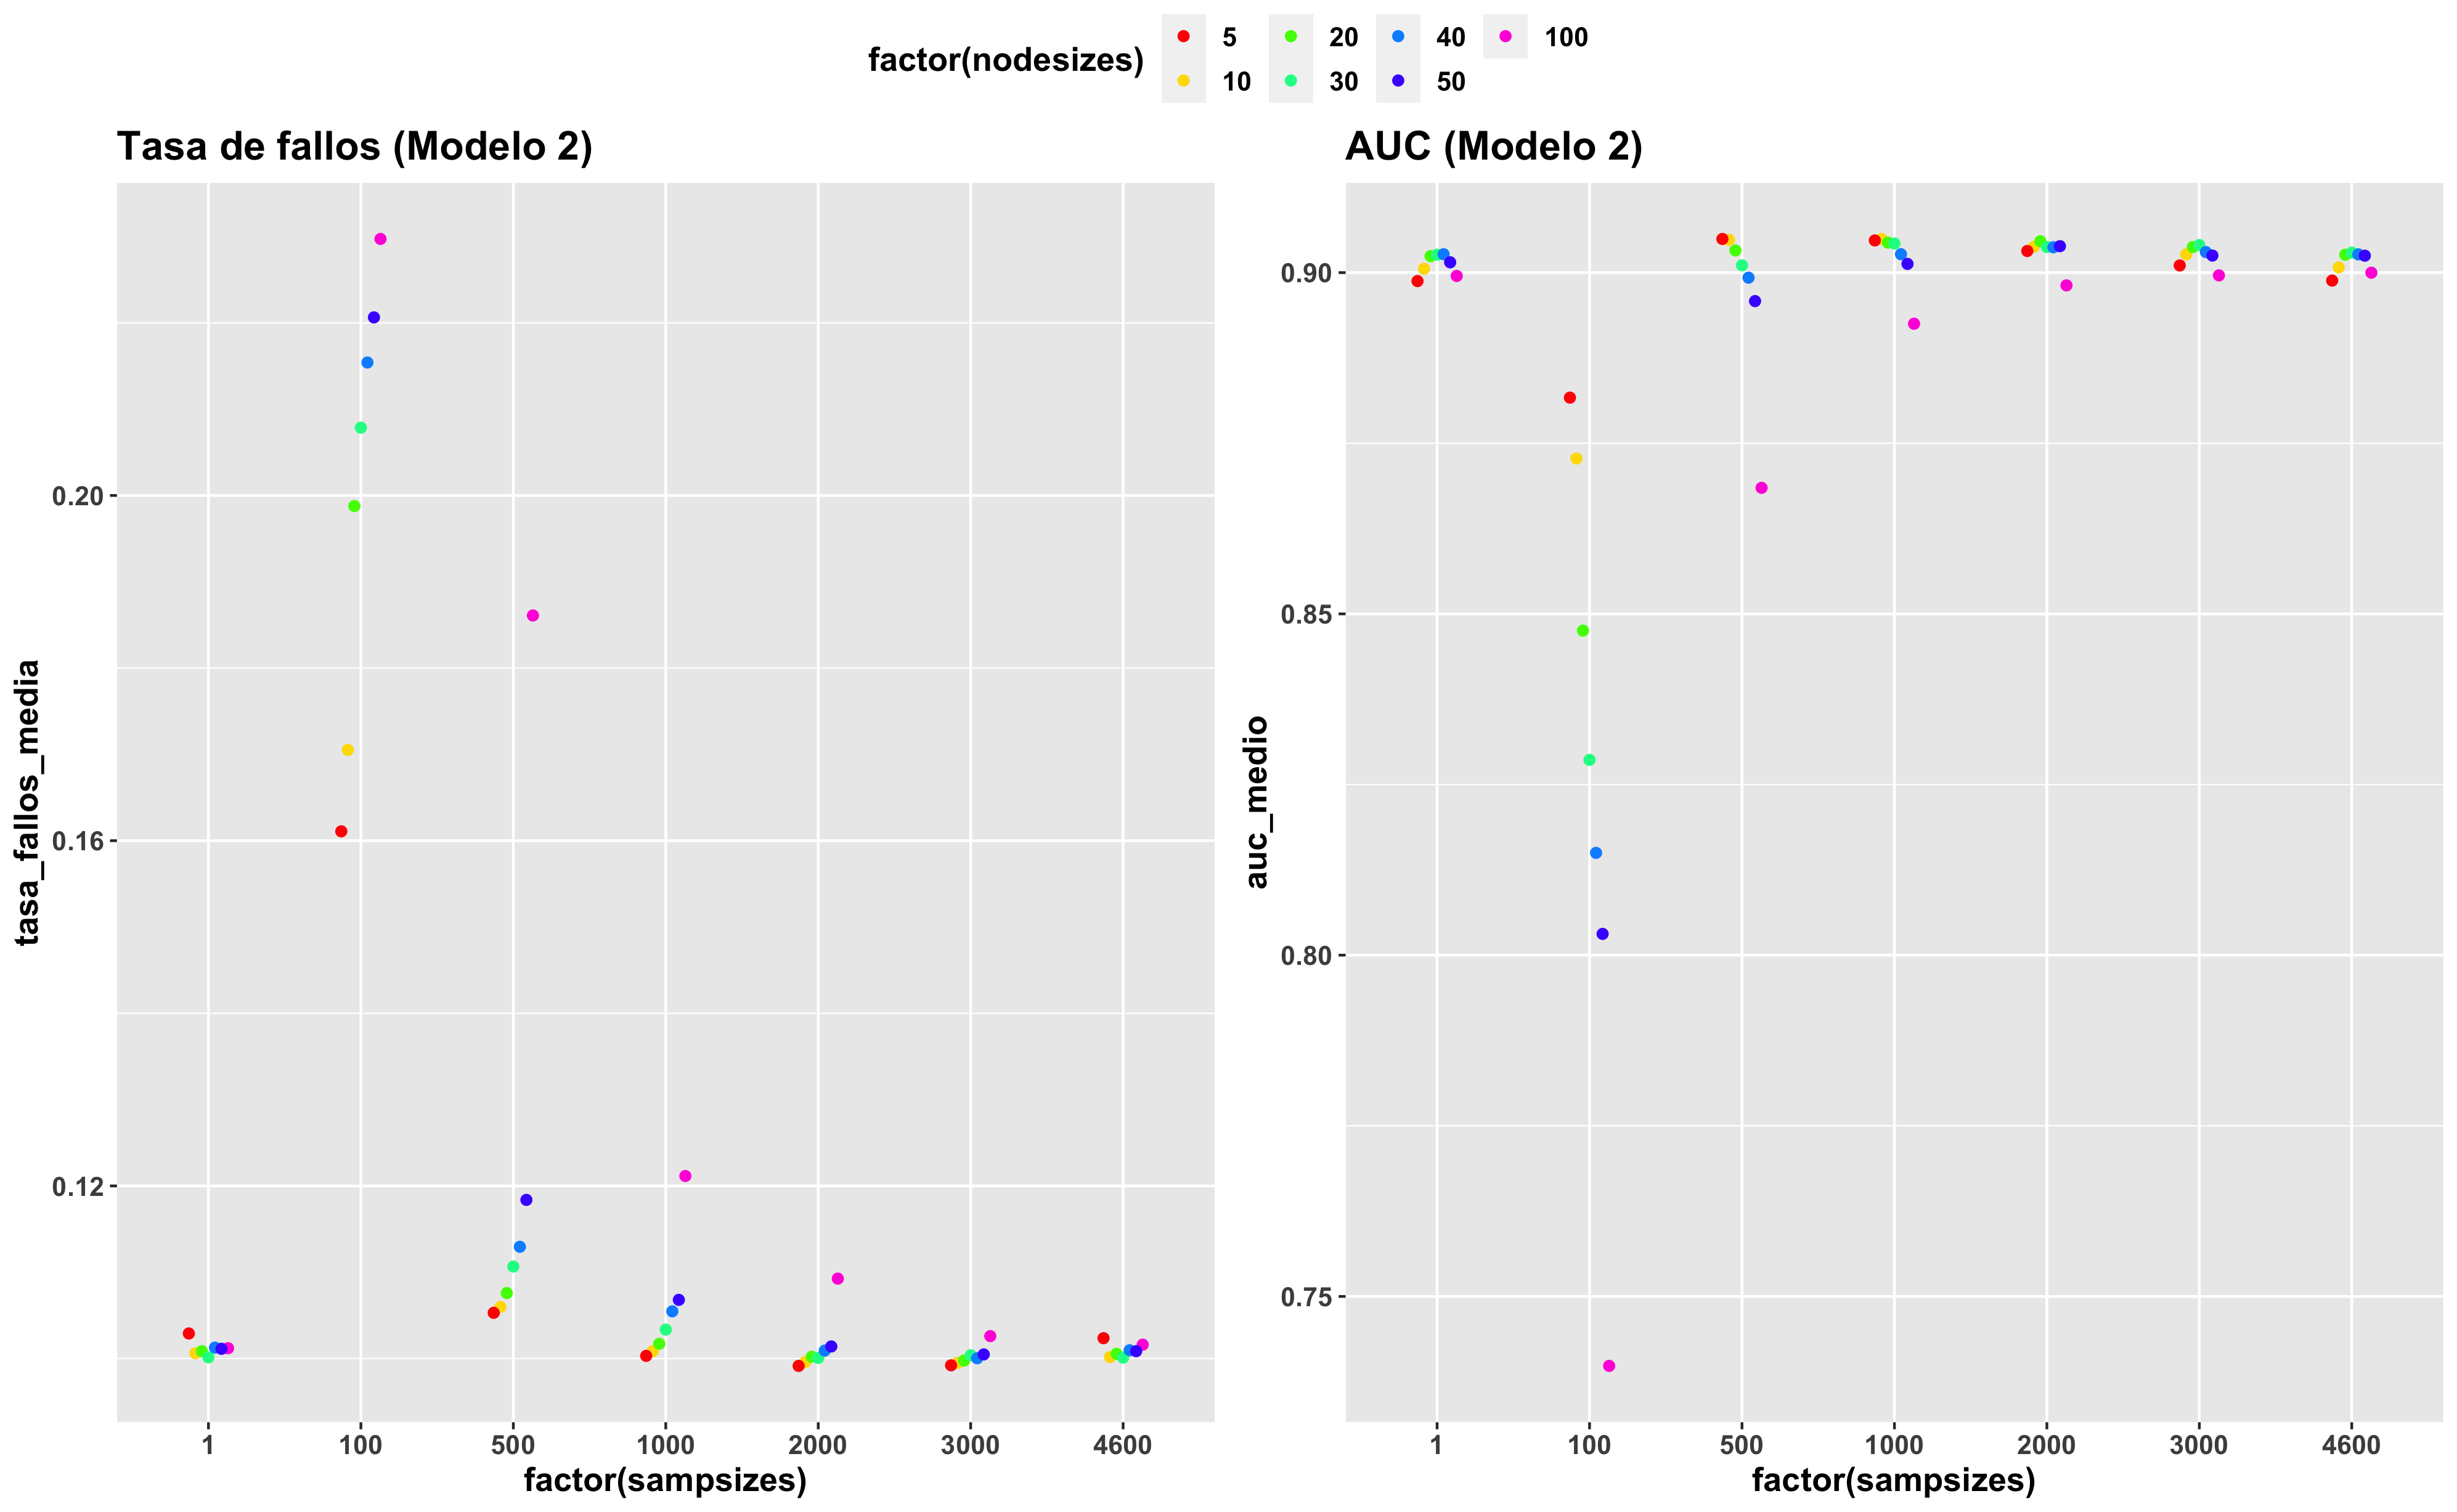
\includegraphics[width=0.99\linewidth,height=0.99\textheight,]{./charts/03_distribucion_auc_tasa_fallos_modelo2} 

}

\caption{Distribucion de la tasa de fallos y AUC por sampsize y nodesize (Modelo 2) (I)}\label{fig:unnamed-chunk-75}
\end{figure}

Nuevamente, nos encontramos con un comportamiento similar al obtenido
con el primer modelo: por un lado, con un valor \emph{nodesize}
moderado/alto (en torno a 20), obtienen buenos resultados, por lo que no
es necesario utilizar árboles demasiado complejos, pues la ganancia
tanto en tasa de fallos como en AUC es ínfima. Por otro lado, y en
relación con \emph{sampsize}, \textbf{no es necesario emplear todas las
observaciones}, sino que con tan solo 500 o 1000 muestras, el modelo
obtiene buenos resultados.

Por tanto, y del mismo modo que en el primer \emph{set} de variables,
\_\_comparamos la diferencia entre un modelo de mayor complejidad (
\emph{nodesize} = 5 ) y de menor complejidad ( \emph{nodesize} = 20 ),
utilizando diferentes tamaños de \emph{sampsize}:

\begin{Shaded}
\begin{Highlighting}[]
\NormalTok{nodesizes}\FloatTok{.2}\NormalTok{ <{-}}\StringTok{ }\KeywordTok{list}\NormalTok{(}\DecValTok{5}\NormalTok{, }\DecValTok{20}\NormalTok{)}
\CommentTok{\#{-}{-} Probamos con un sampsize entre 500 y 2000 observaciones (1 = todas las observaciones)}
\NormalTok{sampsizes}\FloatTok{.2}\NormalTok{ <{-}}\StringTok{ }\KeywordTok{list}\NormalTok{(}\DecValTok{1}\NormalTok{, }\DecValTok{500}\NormalTok{, }\DecValTok{1000}\NormalTok{, }\DecValTok{1500}\NormalTok{, }\DecValTok{2000}\NormalTok{)}
\NormalTok{bagging\_modelo1\_v2 <{-}}\StringTok{ }\KeywordTok{tuneo\_bagging}\NormalTok{(surgical\_dataset, }\DataTypeTok{target =}\NormalTok{ target,}
                                    \DataTypeTok{lista.continua =}\NormalTok{ var\_modelo2,}
                                    \DataTypeTok{nodesizes =}\NormalTok{ nodesizes}\FloatTok{.2}\NormalTok{,}
                                    \DataTypeTok{sampsizes =}\NormalTok{ sampsizes}\FloatTok{.2}\NormalTok{, }\DataTypeTok{mtry =}\NormalTok{ mtry}\FloatTok{.2}\NormalTok{,}
                                    \DataTypeTok{ntree =}\NormalTok{ n.trees}\FloatTok{.2}\NormalTok{, }\DataTypeTok{grupos =} \DecValTok{5}\NormalTok{, }\DataTypeTok{repe =} \DecValTok{10}\NormalTok{,}
                                    \DataTypeTok{show\_nrnodes =} \StringTok{"yes"}\NormalTok{)}
\end{Highlighting}
\end{Shaded}

\begin{figure}[h!]

{\centering 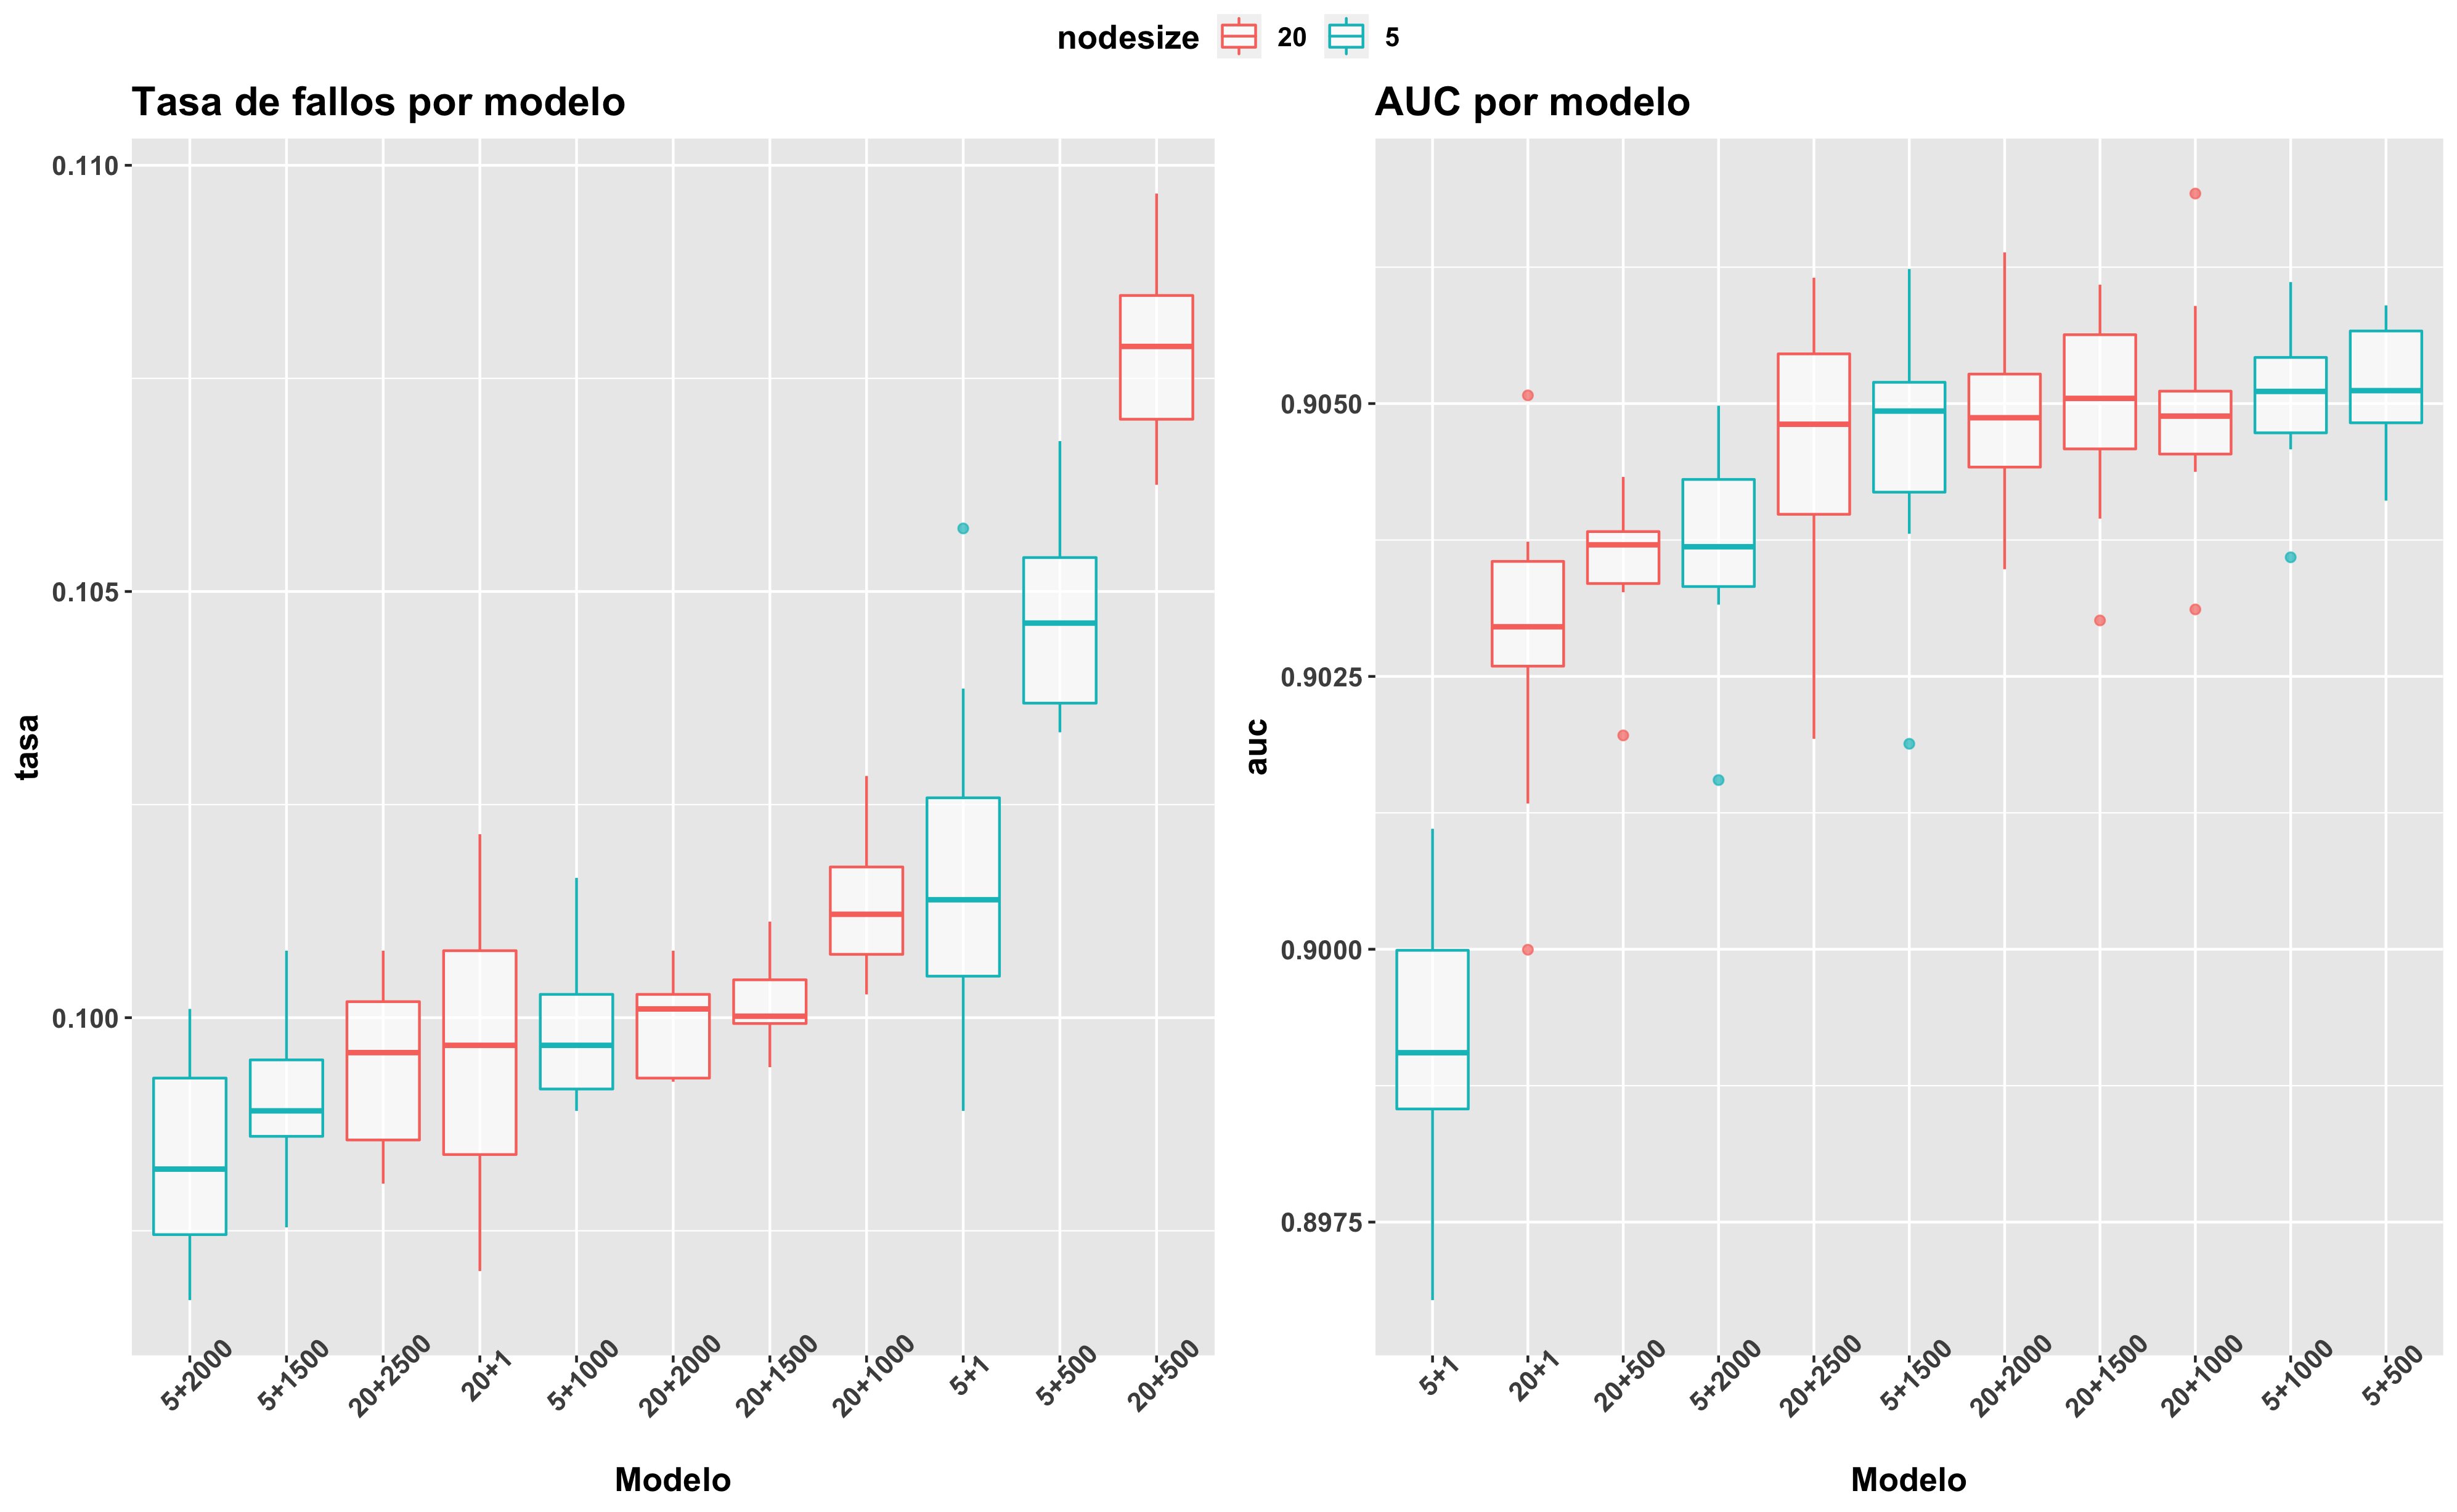
\includegraphics[width=0.99\linewidth,height=0.99\textheight,]{./charts/03_distribucion_auc_tasa_fallos_modelo2_comp} 

}

\caption{Distribucion de la tasa de fallos y AUC por sampsize y nodesize (Modelo 2) (II)}\label{fig:unnamed-chunk-77}
\end{figure}

De nuevo, el hecho de aumentar la complejidad de los árboles (reduciendo
el valor de \emph{nodesize}), no supone una mejoría relevante al modelo.
A modo de ejemplo, la diferencia en la tasa de fallos entre un modelo
con \emph{nodesize} 5 (5 + 2000) y un modelo con \emph{nodesize} 20 (20
+ 2500), es de apenas unas milésimas de diferencia (del mismo modo
sucede con AUC) ¿Y si aumentamos el valor a 50?

\begin{figure}[h!]

{\centering 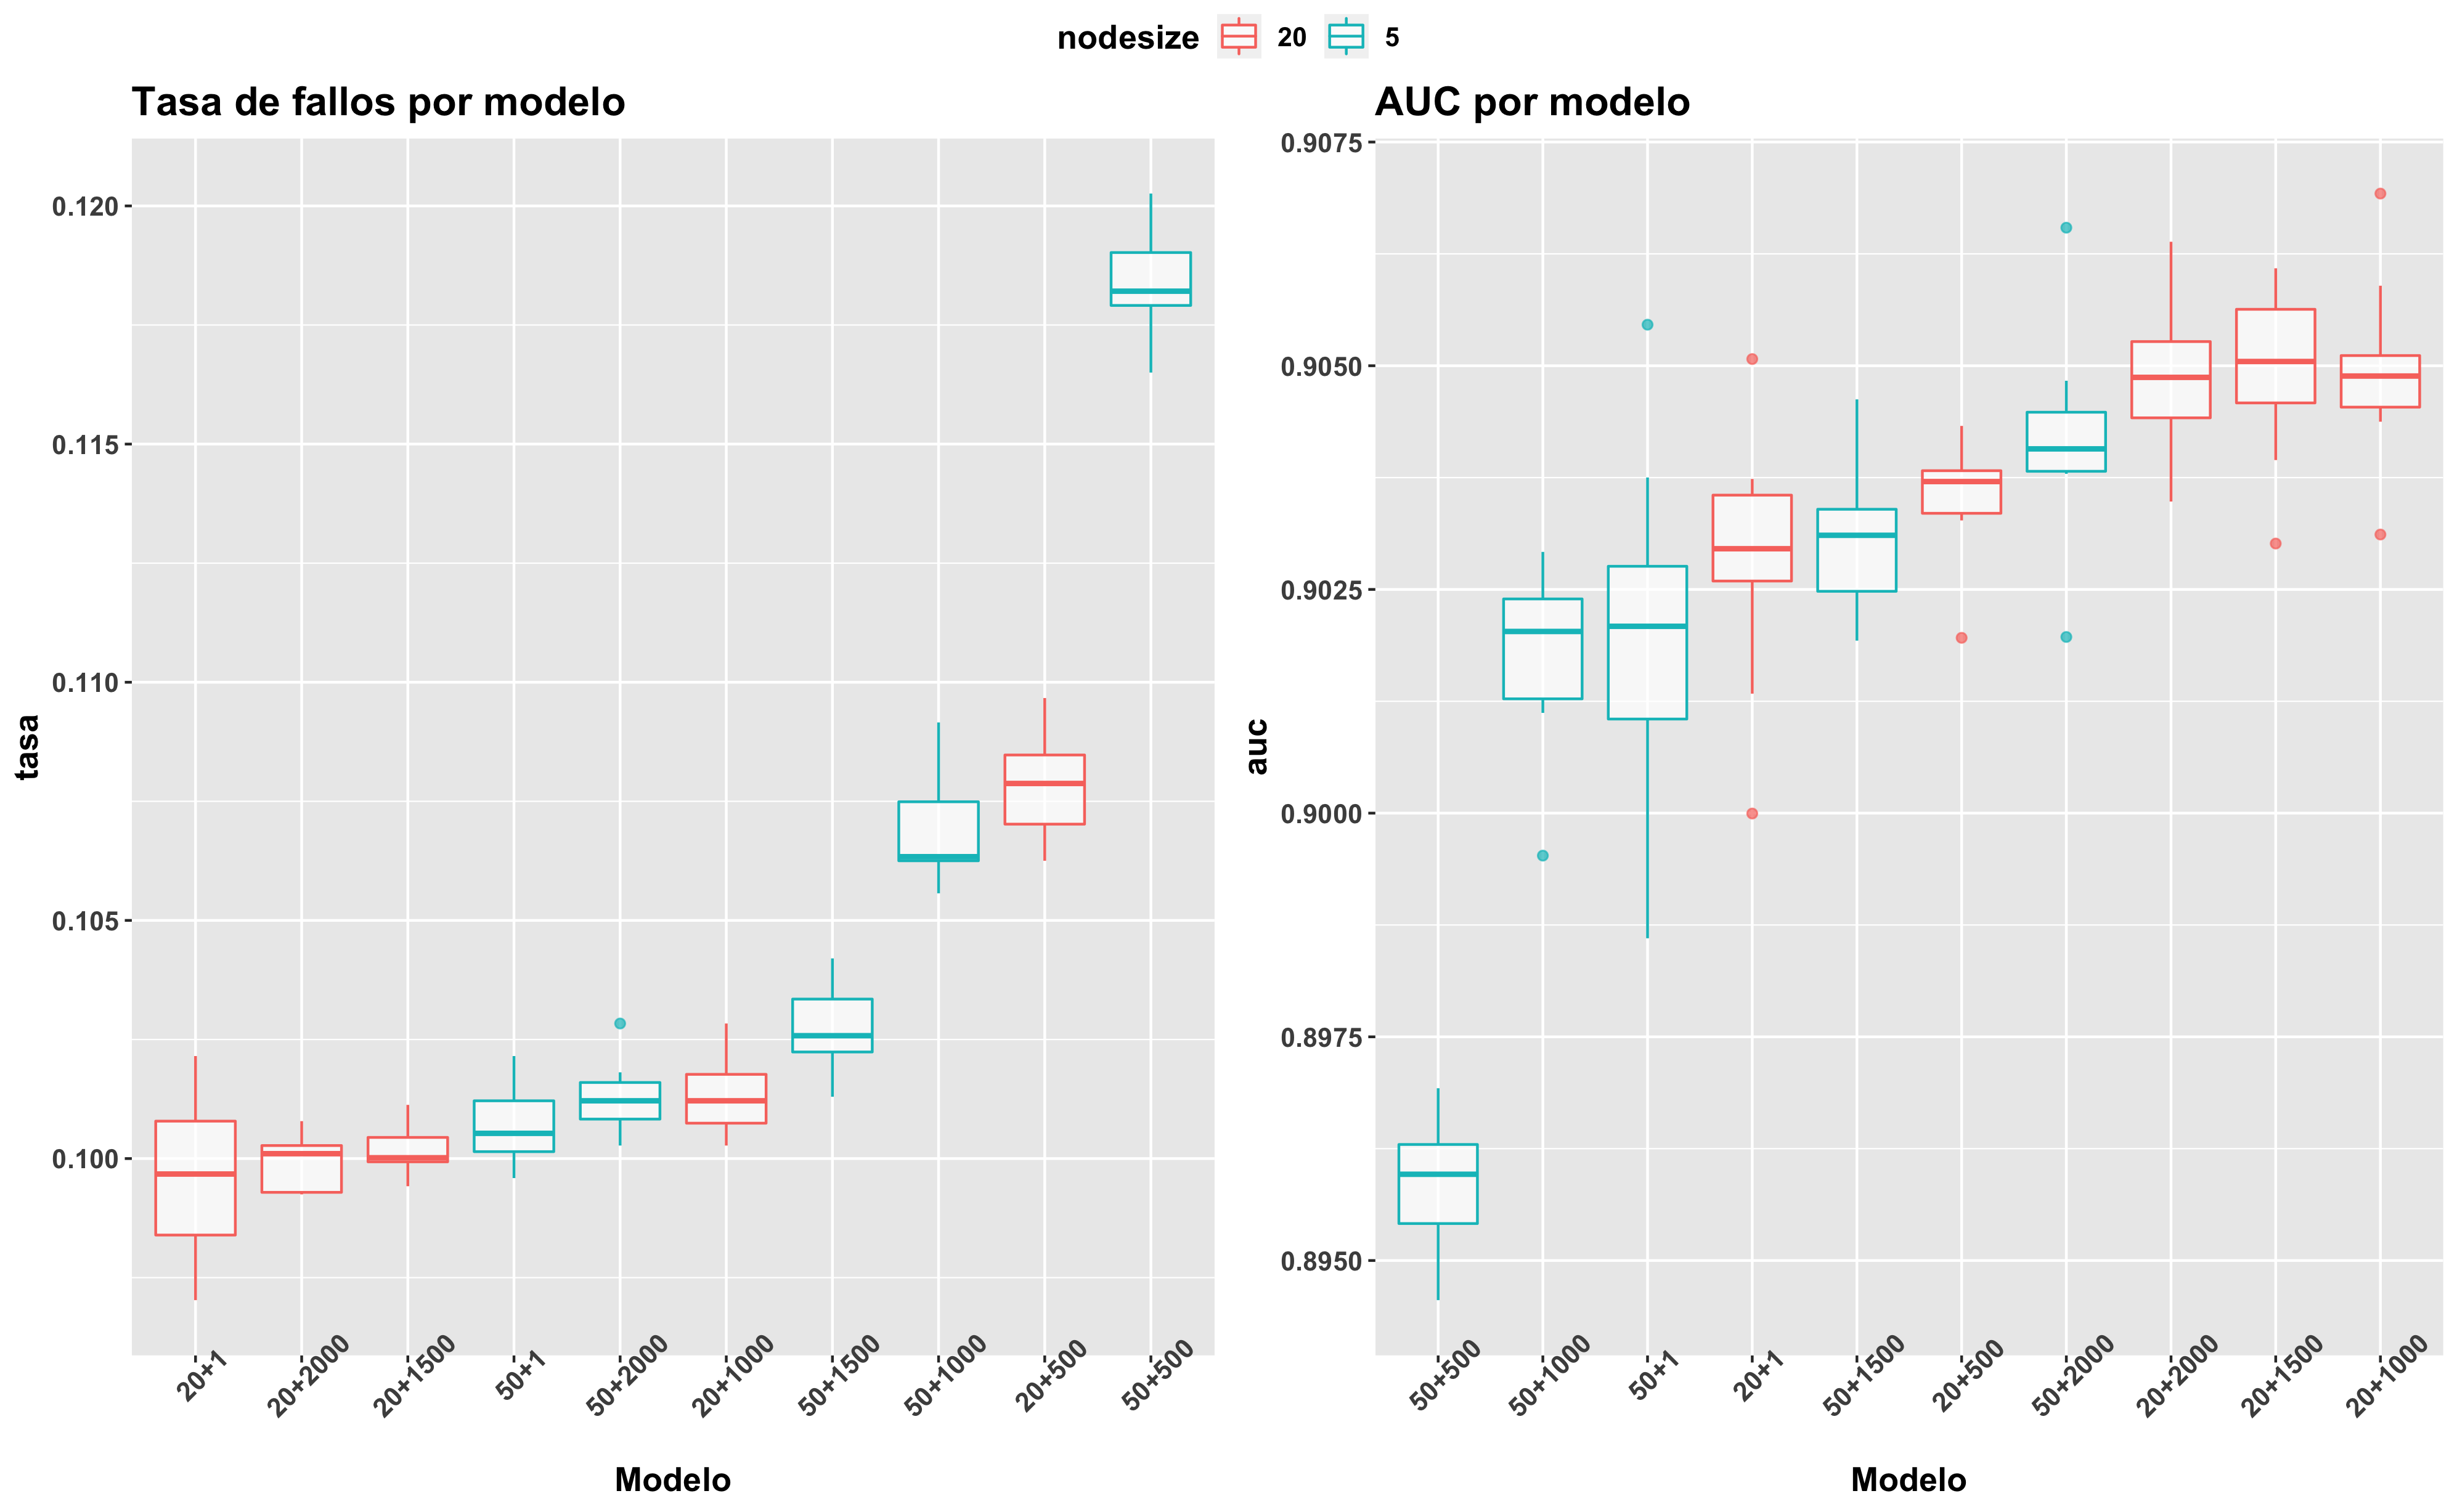
\includegraphics[width=0.99\linewidth,height=0.99\textheight,]{./charts/03_distribucion_auc_tasa_fallos_modelo2_comp_50rep} 

}

\caption{Distribucion de la tasa de fallos y AUC por sampsize y nodesize (Modelo 2) (III)}\label{fig:unnamed-chunk-78}
\end{figure}

En base a la escala de los ejes, la diferencia no es muy significativa.
Sin embargo y por lo general, con un \emph{nodesize} = 50 se requiere un
mayor número de observaciones, al ser árboles de menor complejidad,
mientras que con un \emph{nodesize} menor, en torno a 20, con tan solo
500 o 1000 observaciones se obtienen prácticamente los mismos
resultados.

Por tanto, y del mismo modo que en el primer \emph{set} de variables,
nos decantamos por un \emph{nodesize} de 20 y un tamaño de muestra en
torno a 500-1000 observaciones. Sobre ambos candidatos, probamos de
nuevo con una validación cruzada de 10 grupos y 20 repeticiones:

\begin{figure}[h!]

{\centering 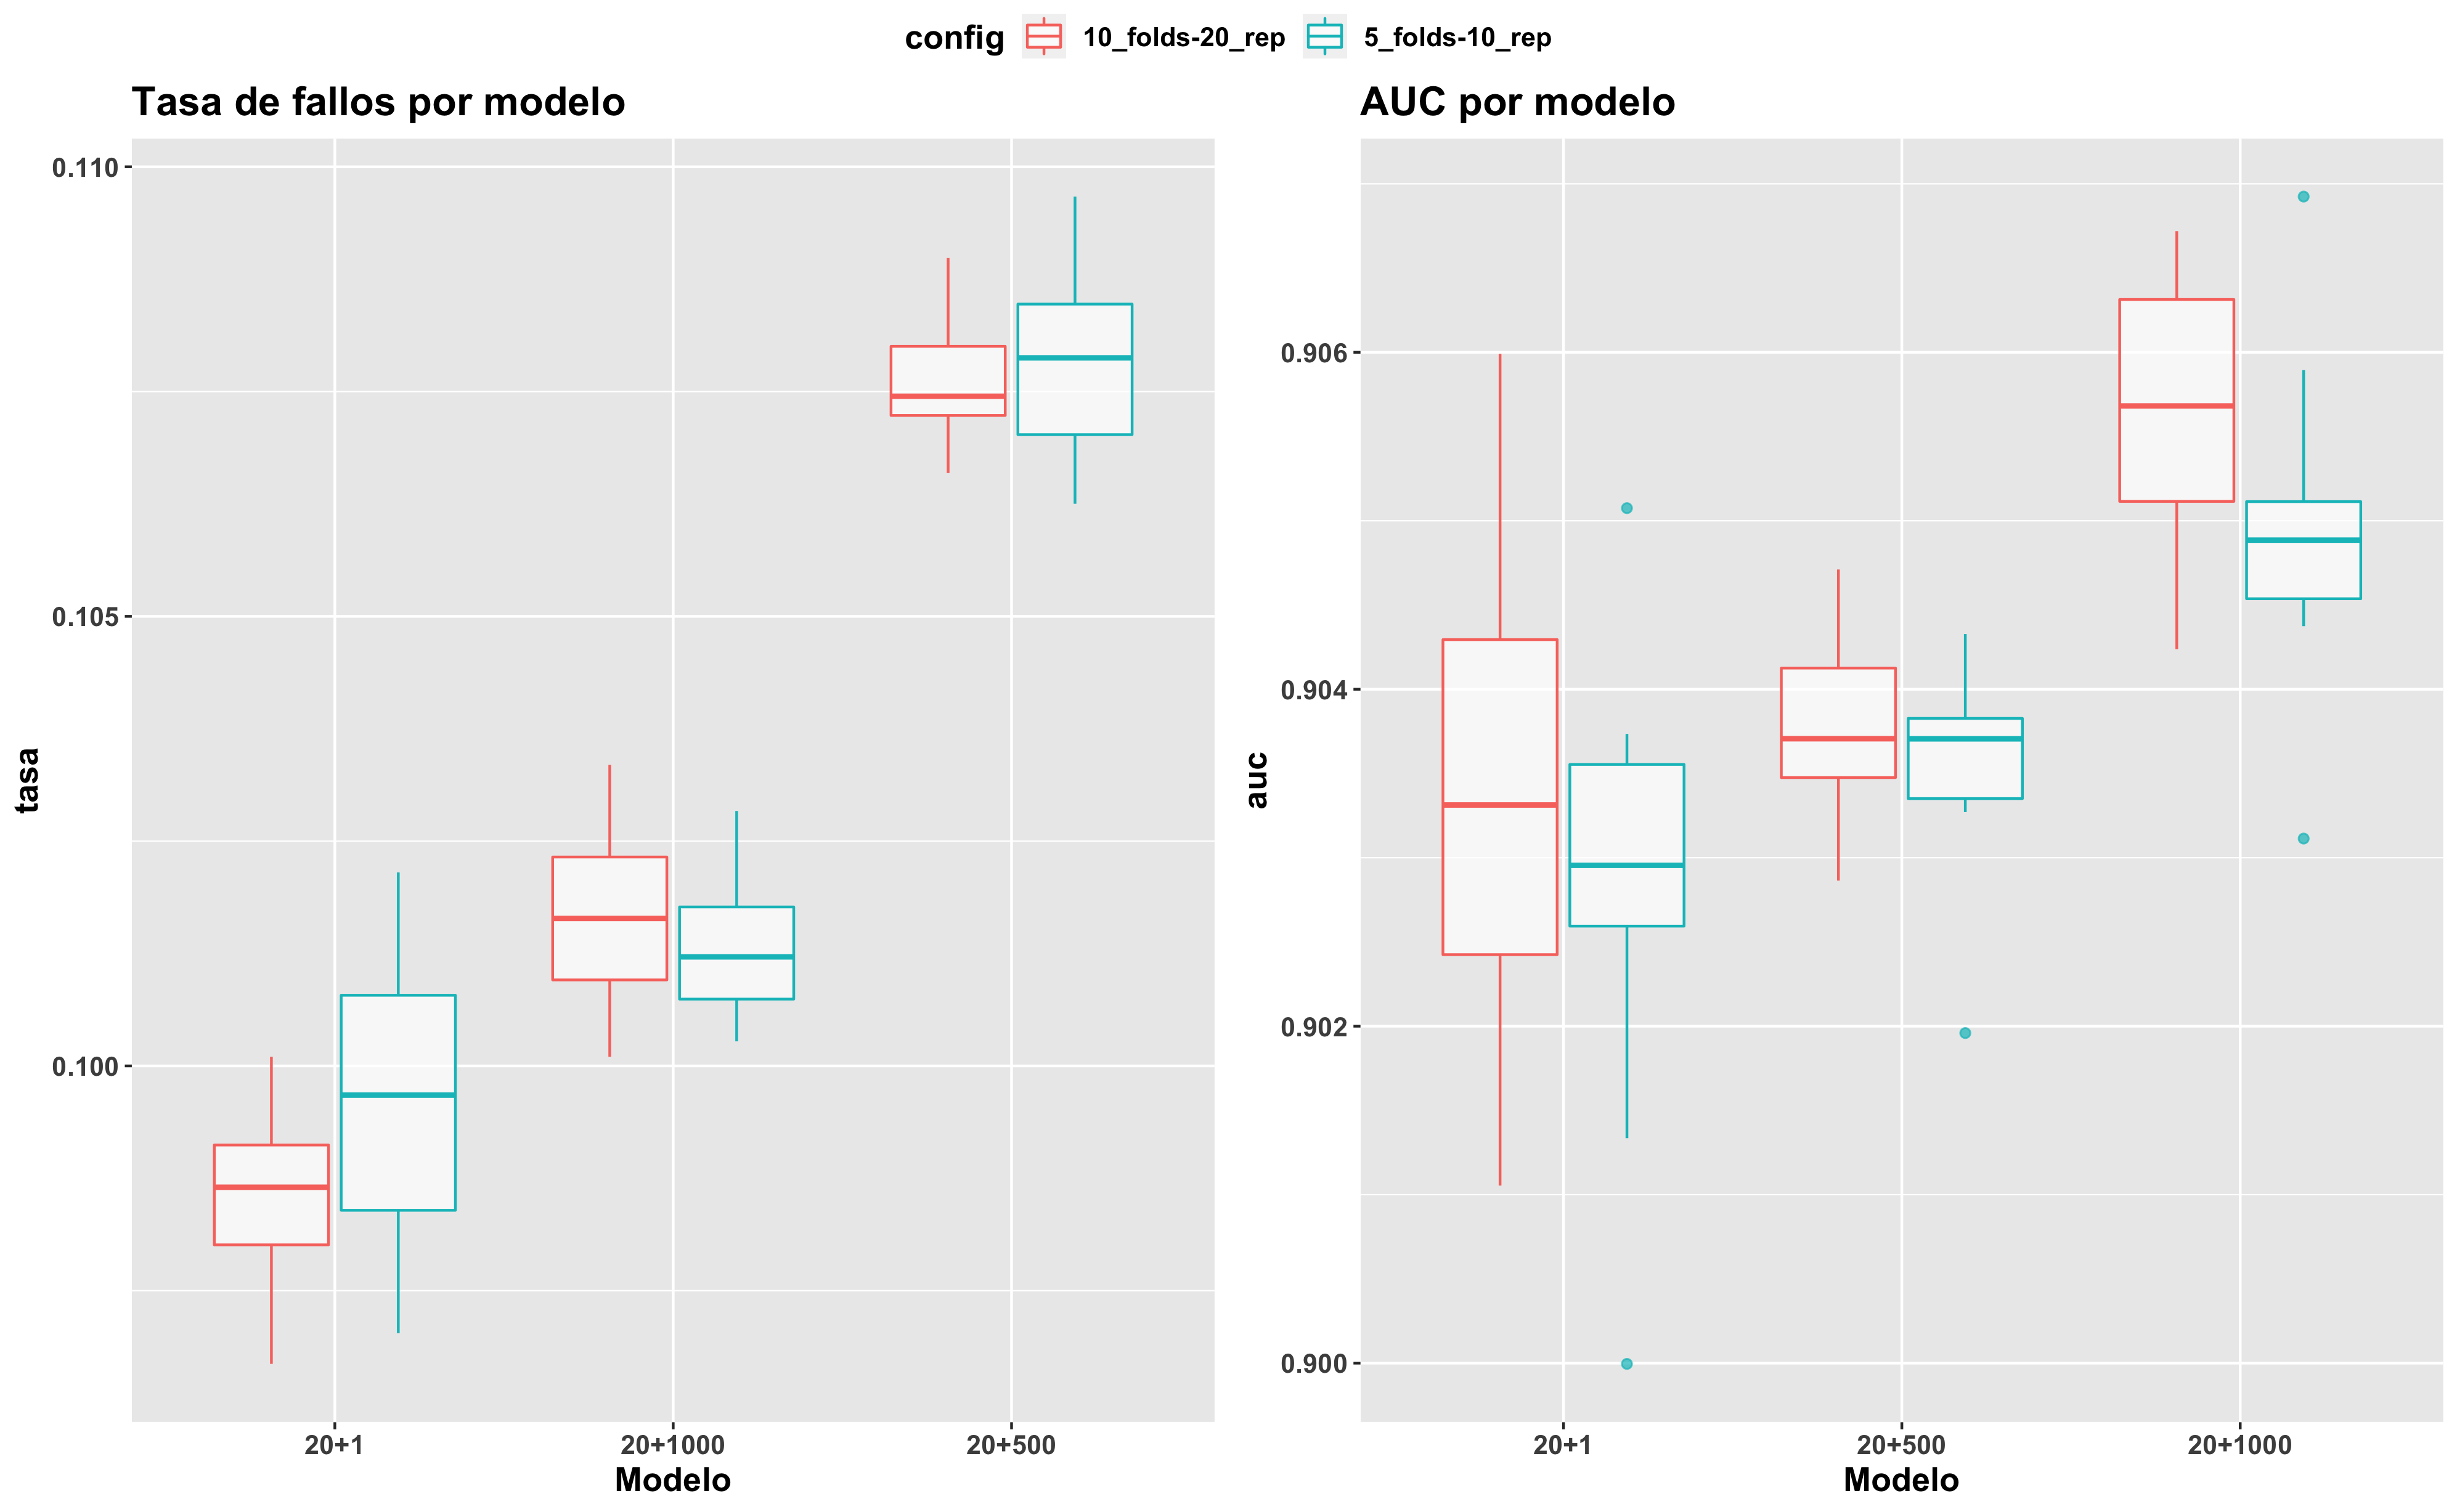
\includegraphics[width=0.99\linewidth,height=0.99\textheight,]{./charts/bagging/bis_03_comparacion_final_modelo2_5_10_folds} 

}

\caption{Distribucion de la tasa de fallos y AUC (Modelo 2) aumentando grupos y repeticiones}\label{fig:unnamed-chunk-79}
\end{figure}

Incluso aumentando el número de grupos, el orden de los modelos se
mantiene prácticamente igual. En conclusión, \textbf{nos decantamos por
la misma configuración que con el primer \emph{set} de variables}:
\emph{nodesize} 20 y \emph{sampsize} 1000.

\textbf{RESUMEN \emph{bagging}}:

\begin{enumerate}
\def\labelenumi{\arabic{enumi}.}
\tightlist
\item
  modelo 1: \emph{nodesize} = 20 y \emph{sampsize} = 1000.
\item
  modelo 2: \emph{nodesize} = 20 y \emph{sampsize} = 1000.
\end{enumerate}

\hypertarget{modelo-sin-reemplazamiento}{%
\subsection{7.4 Modelo sin
reemplazamiento}\label{modelo-sin-reemplazamiento}}

Una vez tuneados ambos \emph{sets} de variables, veamos la diferencia
entre un modelo con \emph{sampsize} con reemplazamiento y sin
reemplazamiento:

\begin{Shaded}
\begin{Highlighting}[]
\CommentTok{\#{-}{-} ¿Y si lo probamos sin reemplazamiento? Probamos con el mejor modelo en terminos de AUC (modelo 1)}
\NormalTok{bagging\_modelo\_sin\_reemp <{-}}\StringTok{ }\KeywordTok{tuneo\_bagging}\NormalTok{(surgical\_dataset, }\DataTypeTok{target =}\NormalTok{ target,}
                                   \DataTypeTok{lista.continua =}\NormalTok{ var\_modelo1, }\DataTypeTok{nodesizes =} \DecValTok{20}\NormalTok{, }
                                   \DataTypeTok{sampsizes =} \DecValTok{1000}\NormalTok{, }\DataTypeTok{mtry =}\NormalTok{ mtry}\FloatTok{.1}\NormalTok{, }\DataTypeTok{ntree =}\NormalTok{ n.trees}\FloatTok{.1}\NormalTok{, }
                                   \DataTypeTok{grupos =} \DecValTok{5}\NormalTok{, }\DataTypeTok{repe =} \DecValTok{10}\NormalTok{, }\DataTypeTok{replace =} \OtherTok{FALSE}\NormalTok{)}
\end{Highlighting}
\end{Shaded}

\begin{figure}[h!]

{\centering 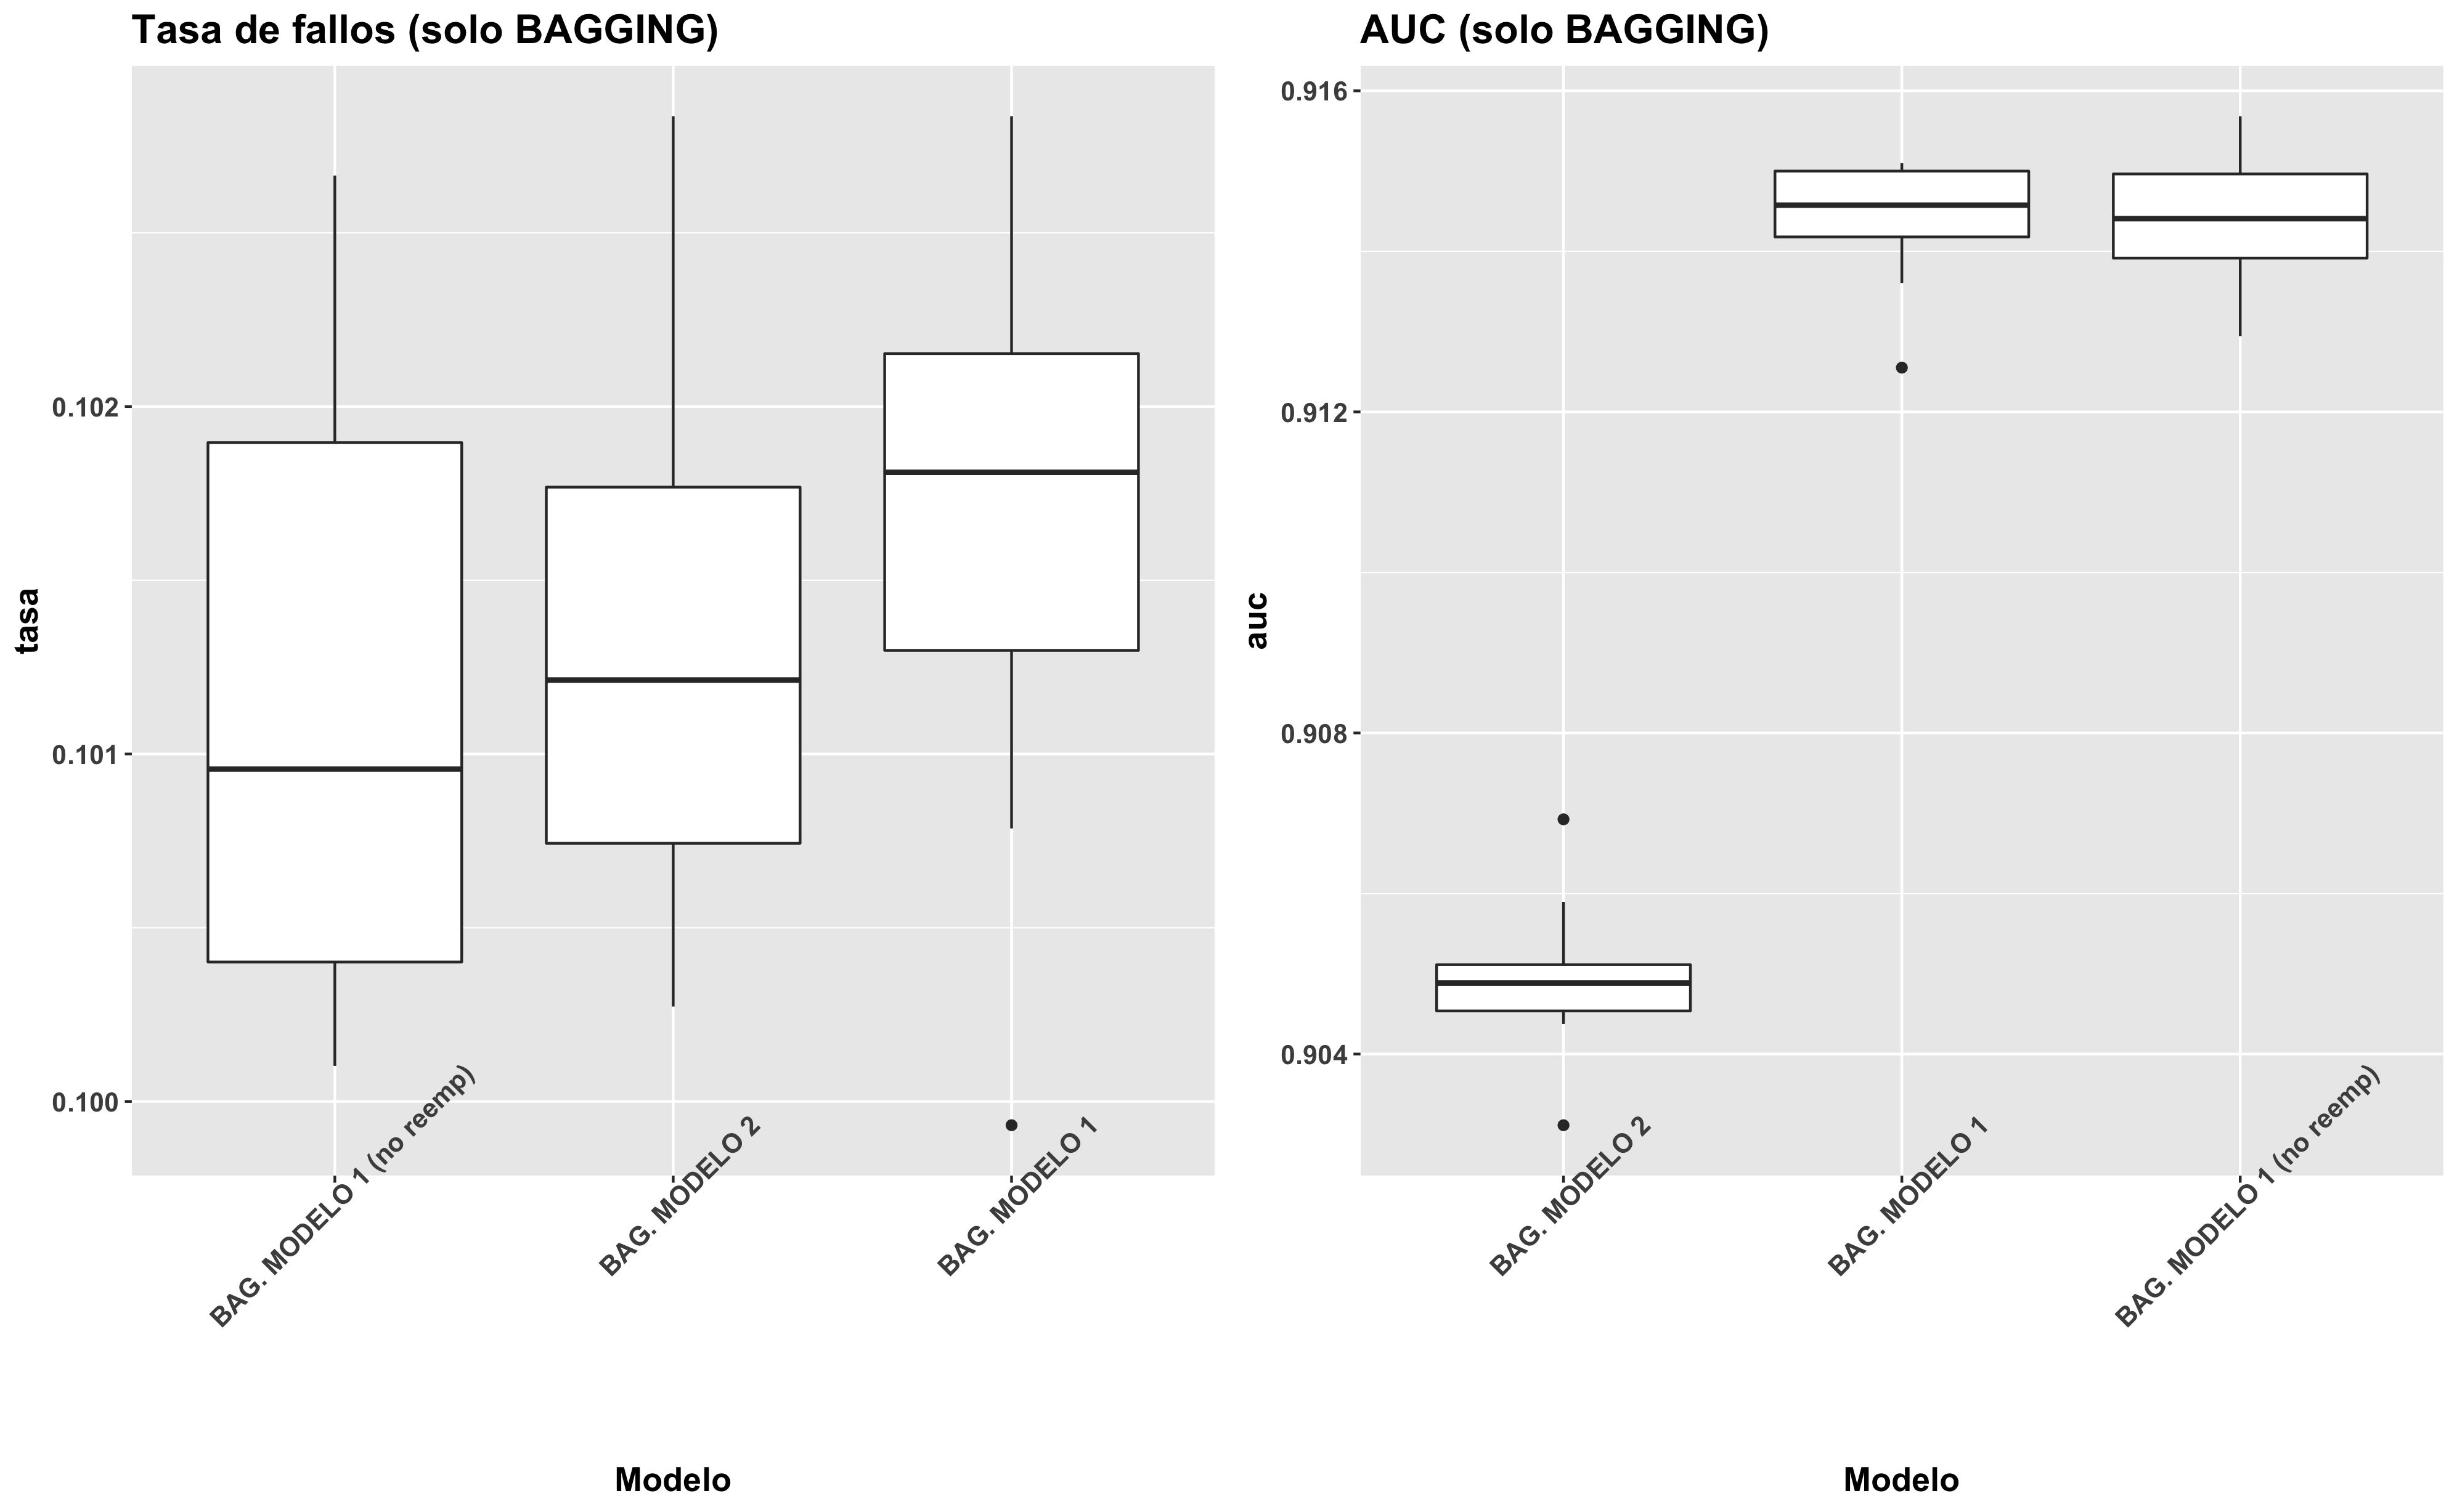
\includegraphics[width=0.99\linewidth,height=0.99\textheight,]{./charts/bagging/03_comparacion_final_bagging} 

}

\caption{Distribucion de la tasa de fallos y AUC con y sin reemplazamiento}\label{fig:unnamed-chunk-81}
\end{figure}

A simple vista, no existe diferencia entre modelos con o sin
reemplazamiento en \emph{sampsize}. Por otro lado, y del mismo modo que
sucedía con el modelo de red, no existe apenas diferencia entre el
primer \emph{set} con 5 variables y el segundo \emph{set} con 4, tan
solo de 0.01 en el caso del AUC.

\hypertarget{comparaciuxf3n-final-1}{%
\subsection{7.5 Comparación final}\label{comparaciuxf3n-final-1}}

Finalmente, realizamos la comparación final de ambos modelos
\emph{bagging} con los datos \emph{test}:

\begin{verbatim}
##                 modelo precision sensibilidad especificidad valor_pred_pos
## 1 Modelo 1 (BIC TOP 5)    0.9010       0.9214        0.8966         0.6589
## 2     Modelo 2 (top 4)    0.9019       0.9468        0.8928         0.6424
##   valor_pred_neg
## 1         0.9813
## 2         0.9880
\end{verbatim}

Por lo general, la estadísticas de las predicciones mejoran ligeramente,
aunque se mantienen en la misma línea del modelo de red neuronal: altos
porcentajes de sensibilidad, especificidad y valor predictivo negativo,
aunque el valor predictivo positivo se sitúa en torno al 64-65 \%,
aproximadamente, lo cual es un indicativo de la presencia de un alto
número de falsos positivos en las predicciones. Además, la diferencia
entre el primer modelo \emph{bagging} (con 5 variables \emph{input}) y
el segundo (con tan solo 4), no es muy relevante en base a las
estadísticas anteriores.

Además, si observamos la distribución de la tasa de fallos y AUC en los
modelos:

\begin{figure}[h!]

{\centering 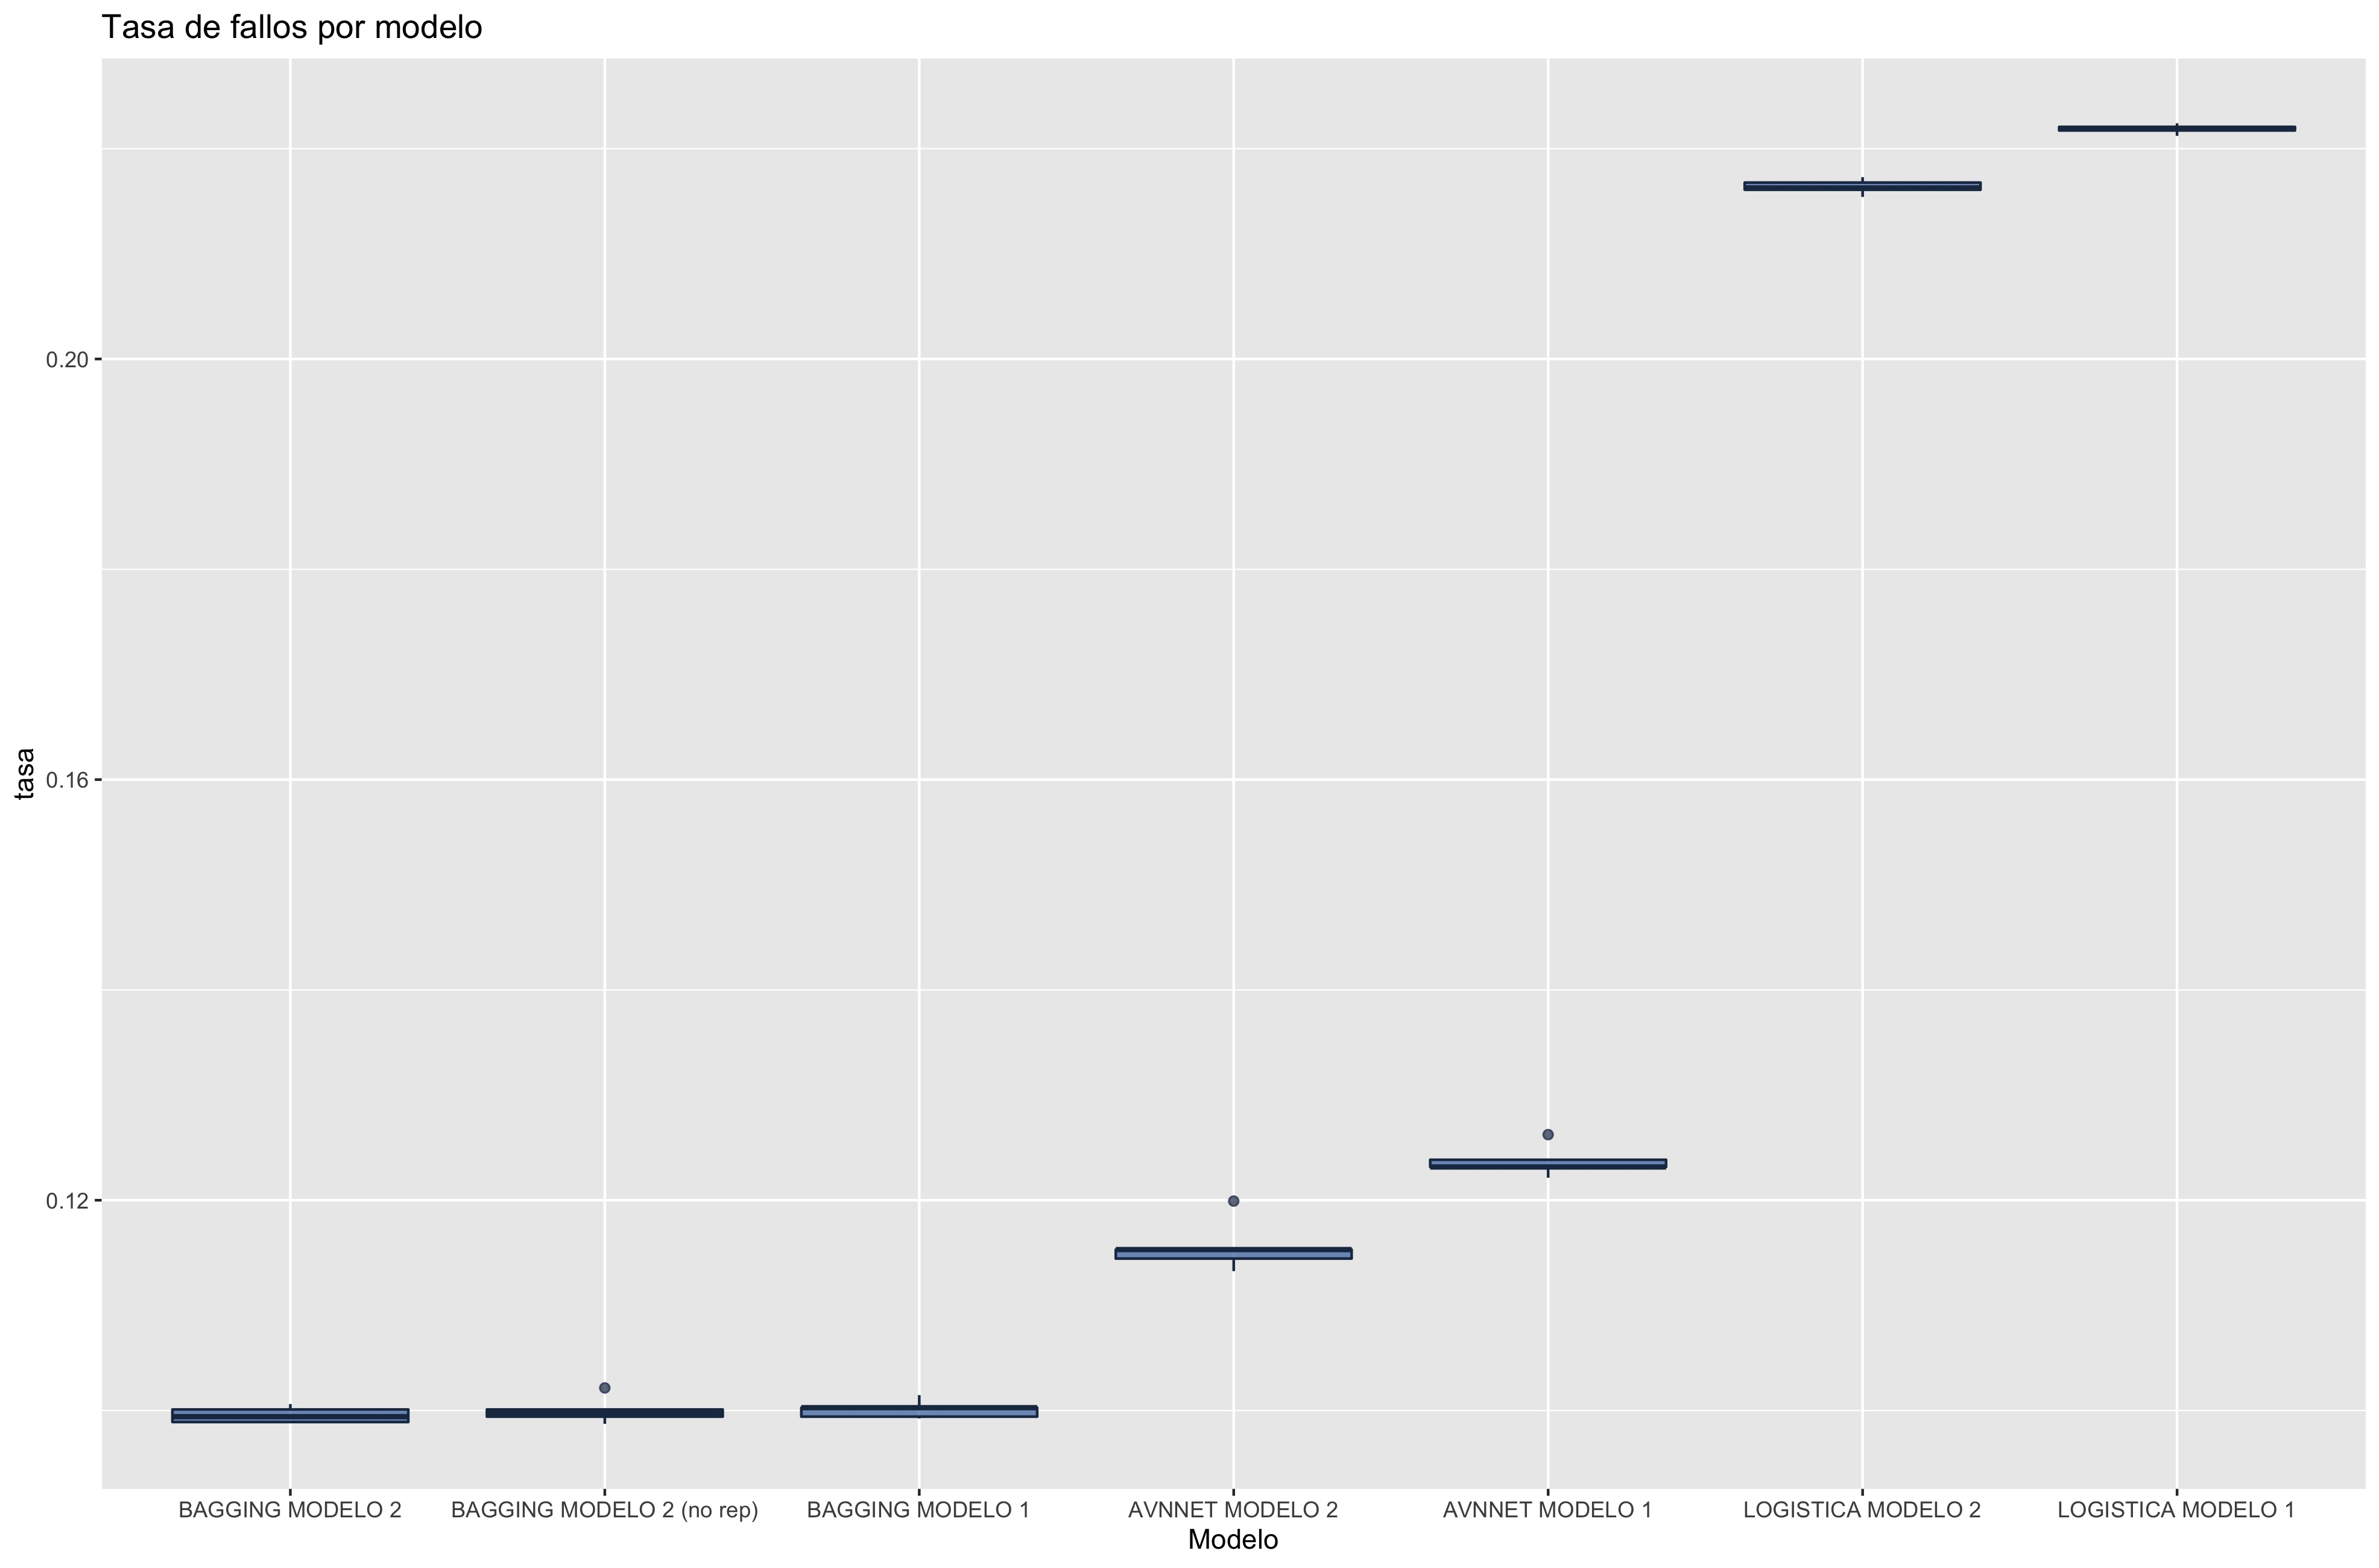
\includegraphics[width=0.99\linewidth,height=0.99\textheight,]{./charts/comparativas/03_log_avnnet_bagging_tasa} 

}

\caption{Comparacion tasa fallos log-avnnet-bagging}\label{fig:unnamed-chunk-83}
\end{figure}
\begin{figure}[h!]

{\centering 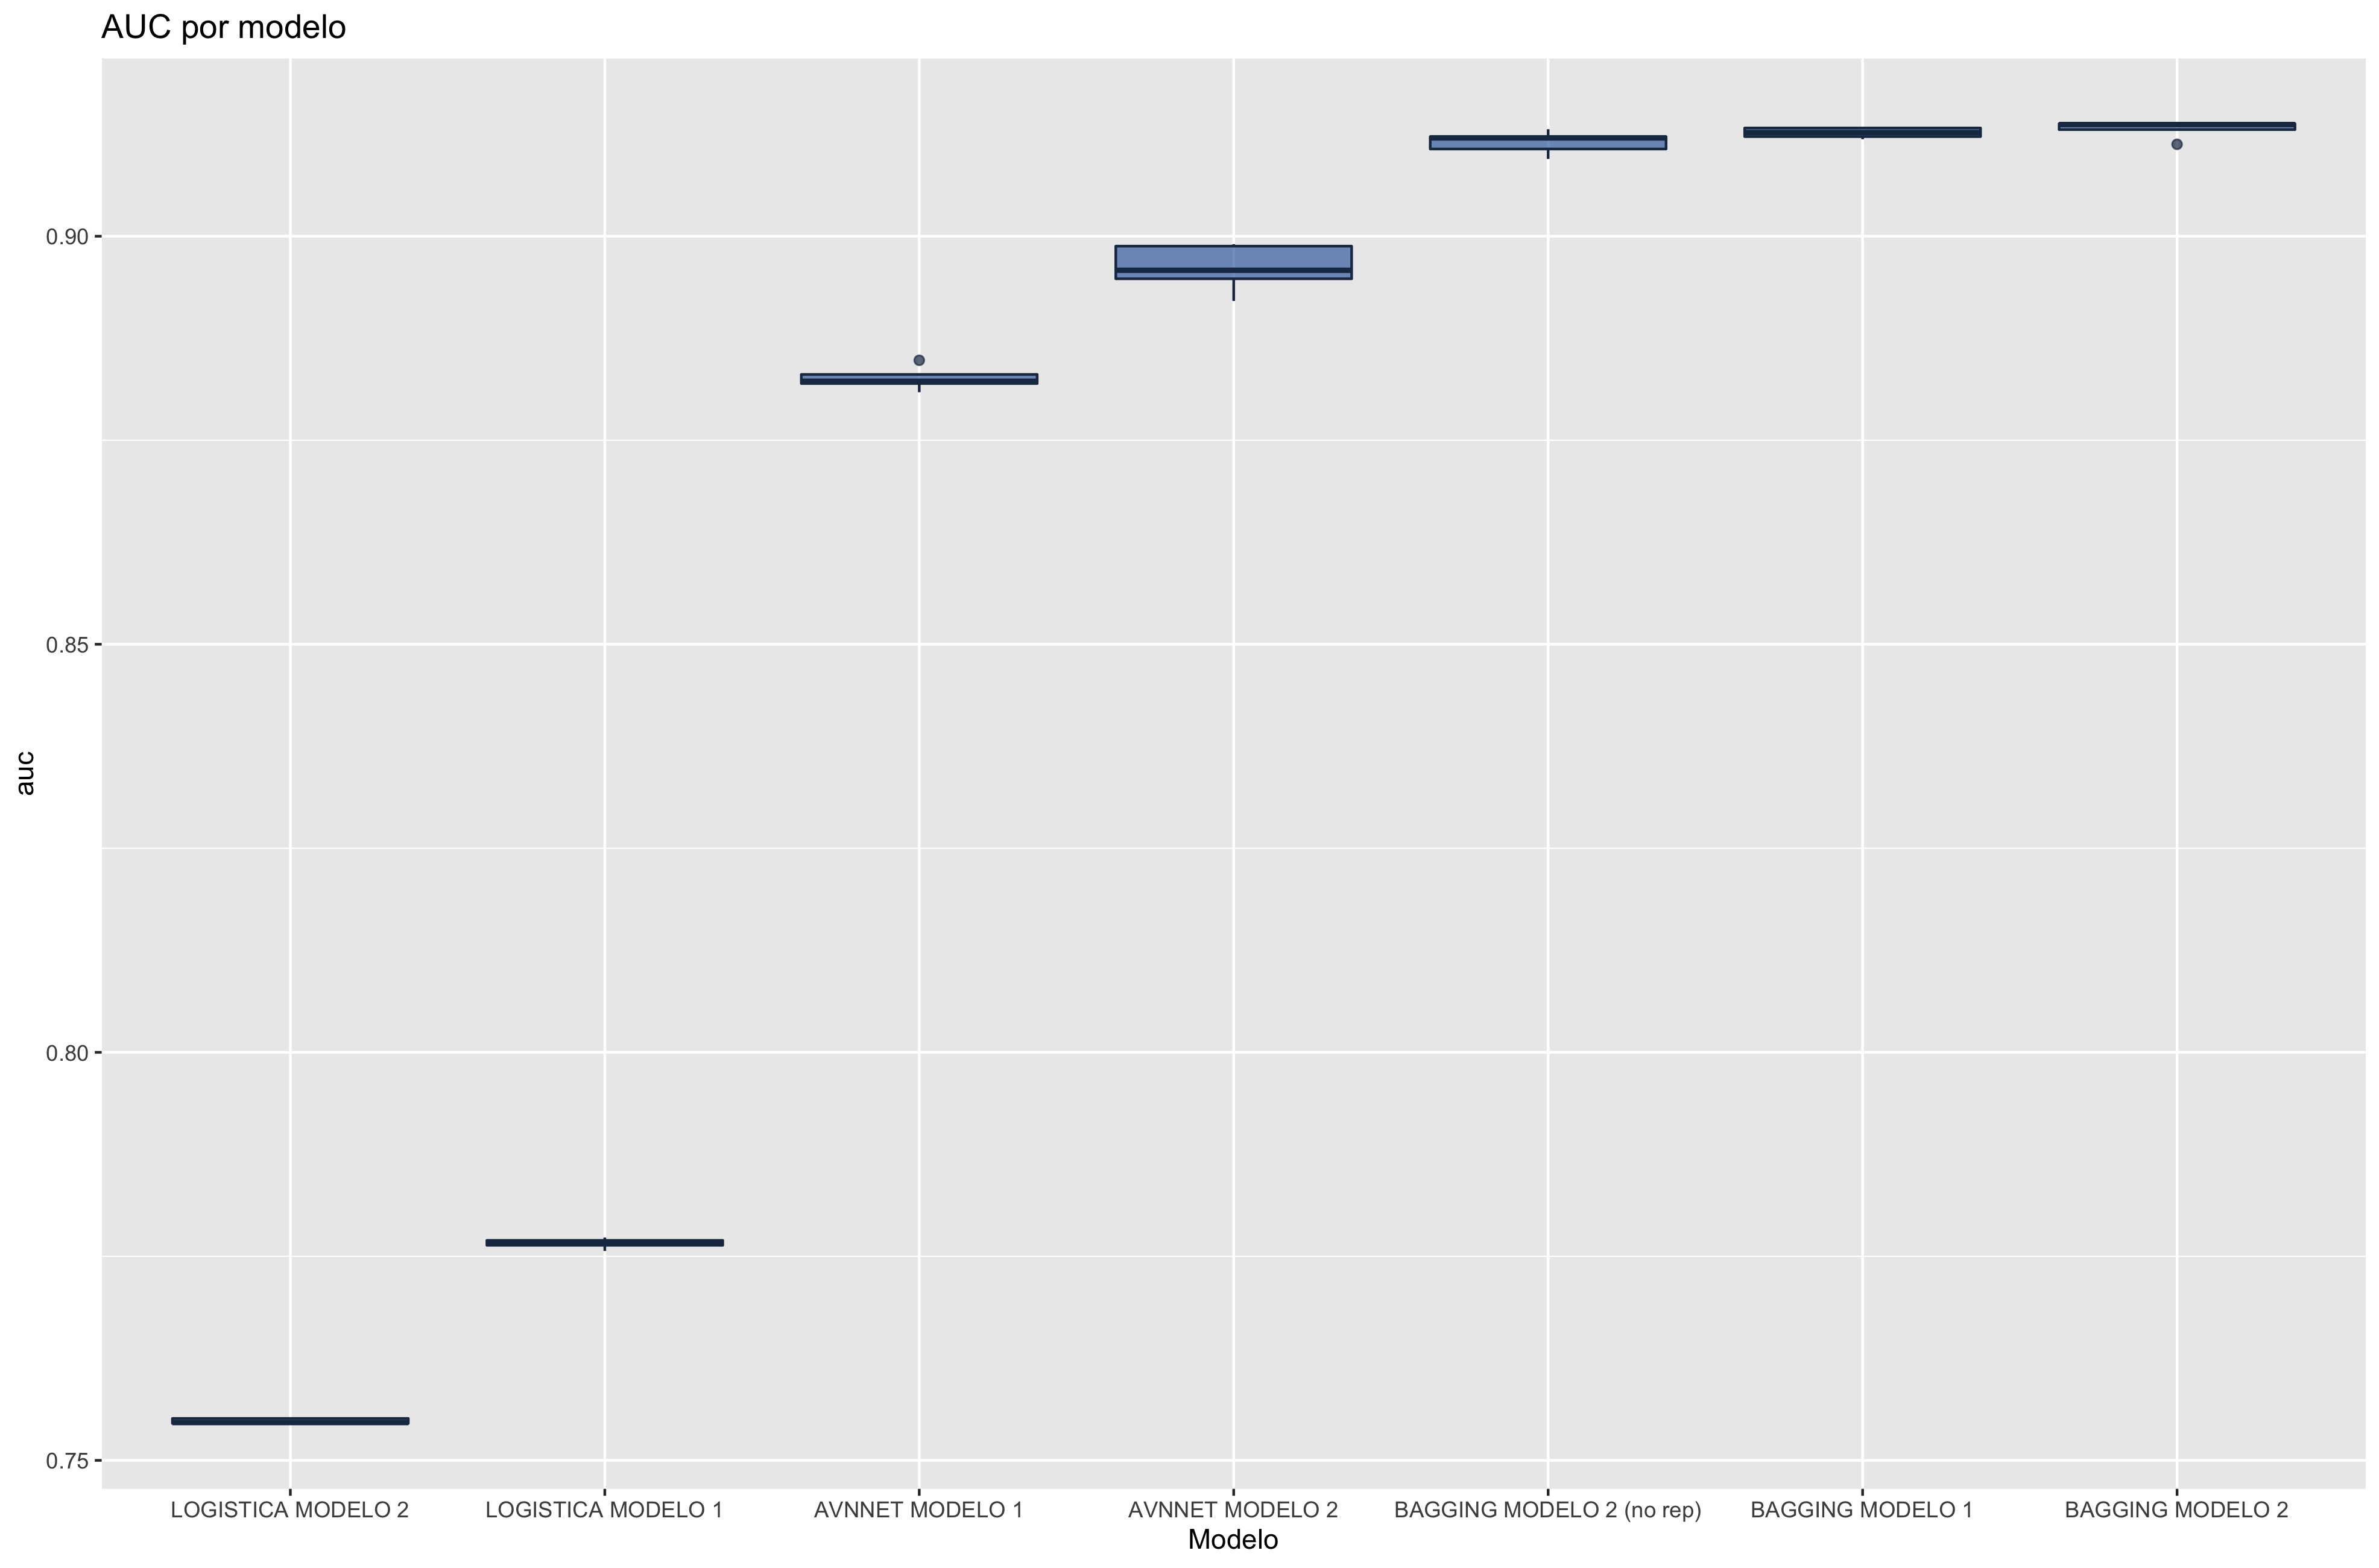
\includegraphics[width=0.99\linewidth,height=0.99\textheight,]{./charts/comparativas/03_log_avnnet_bagging_auc} 

}

\caption{Comparacion AUC log-avnnet-bagging}\label{fig:unnamed-chunk-84}
\end{figure}

De nuevo, la relación no lineal entre las variables \emph{input} se ve
reflejado en los resultados obtenidos tanto en modelos de red como
\emph{bagging}, siendo este último caso el que obtiene mejores
resultados tanto en tasa de fallos como en AUC, aunque la diferencia
(dada la escala de los ejes) no sea muy relevante.

\hypertarget{random-forest}{%
\section{8. Random Forest}\label{random-forest}}

\hypertarget{selecciuxf3n-del-nuxfamero-de-uxe1rboles-y-mtry}{%
\subsection{8.1 Selección del número de árboles y
mtry}\label{selecciuxf3n-del-nuxfamero-de-uxe1rboles-y-mtry}}

Una vez elaborados los modelos \emph{bagging}, y dado que \emph{Random
Forest} si realiza el sorteo de variables por cada división del árbol
¿Con 900 árboles es suficiente? Para comprobarlo, analicemos en ambos
\emph{sets} la evolución del \emph{ratio} de error al variar el
parámetro \emph{mtry}:

\hypertarget{modelo-1-1}{%
\subsubsection{8.1.1 Modelo 1}\label{modelo-1-1}}

\begin{figure}[h!]

{\centering 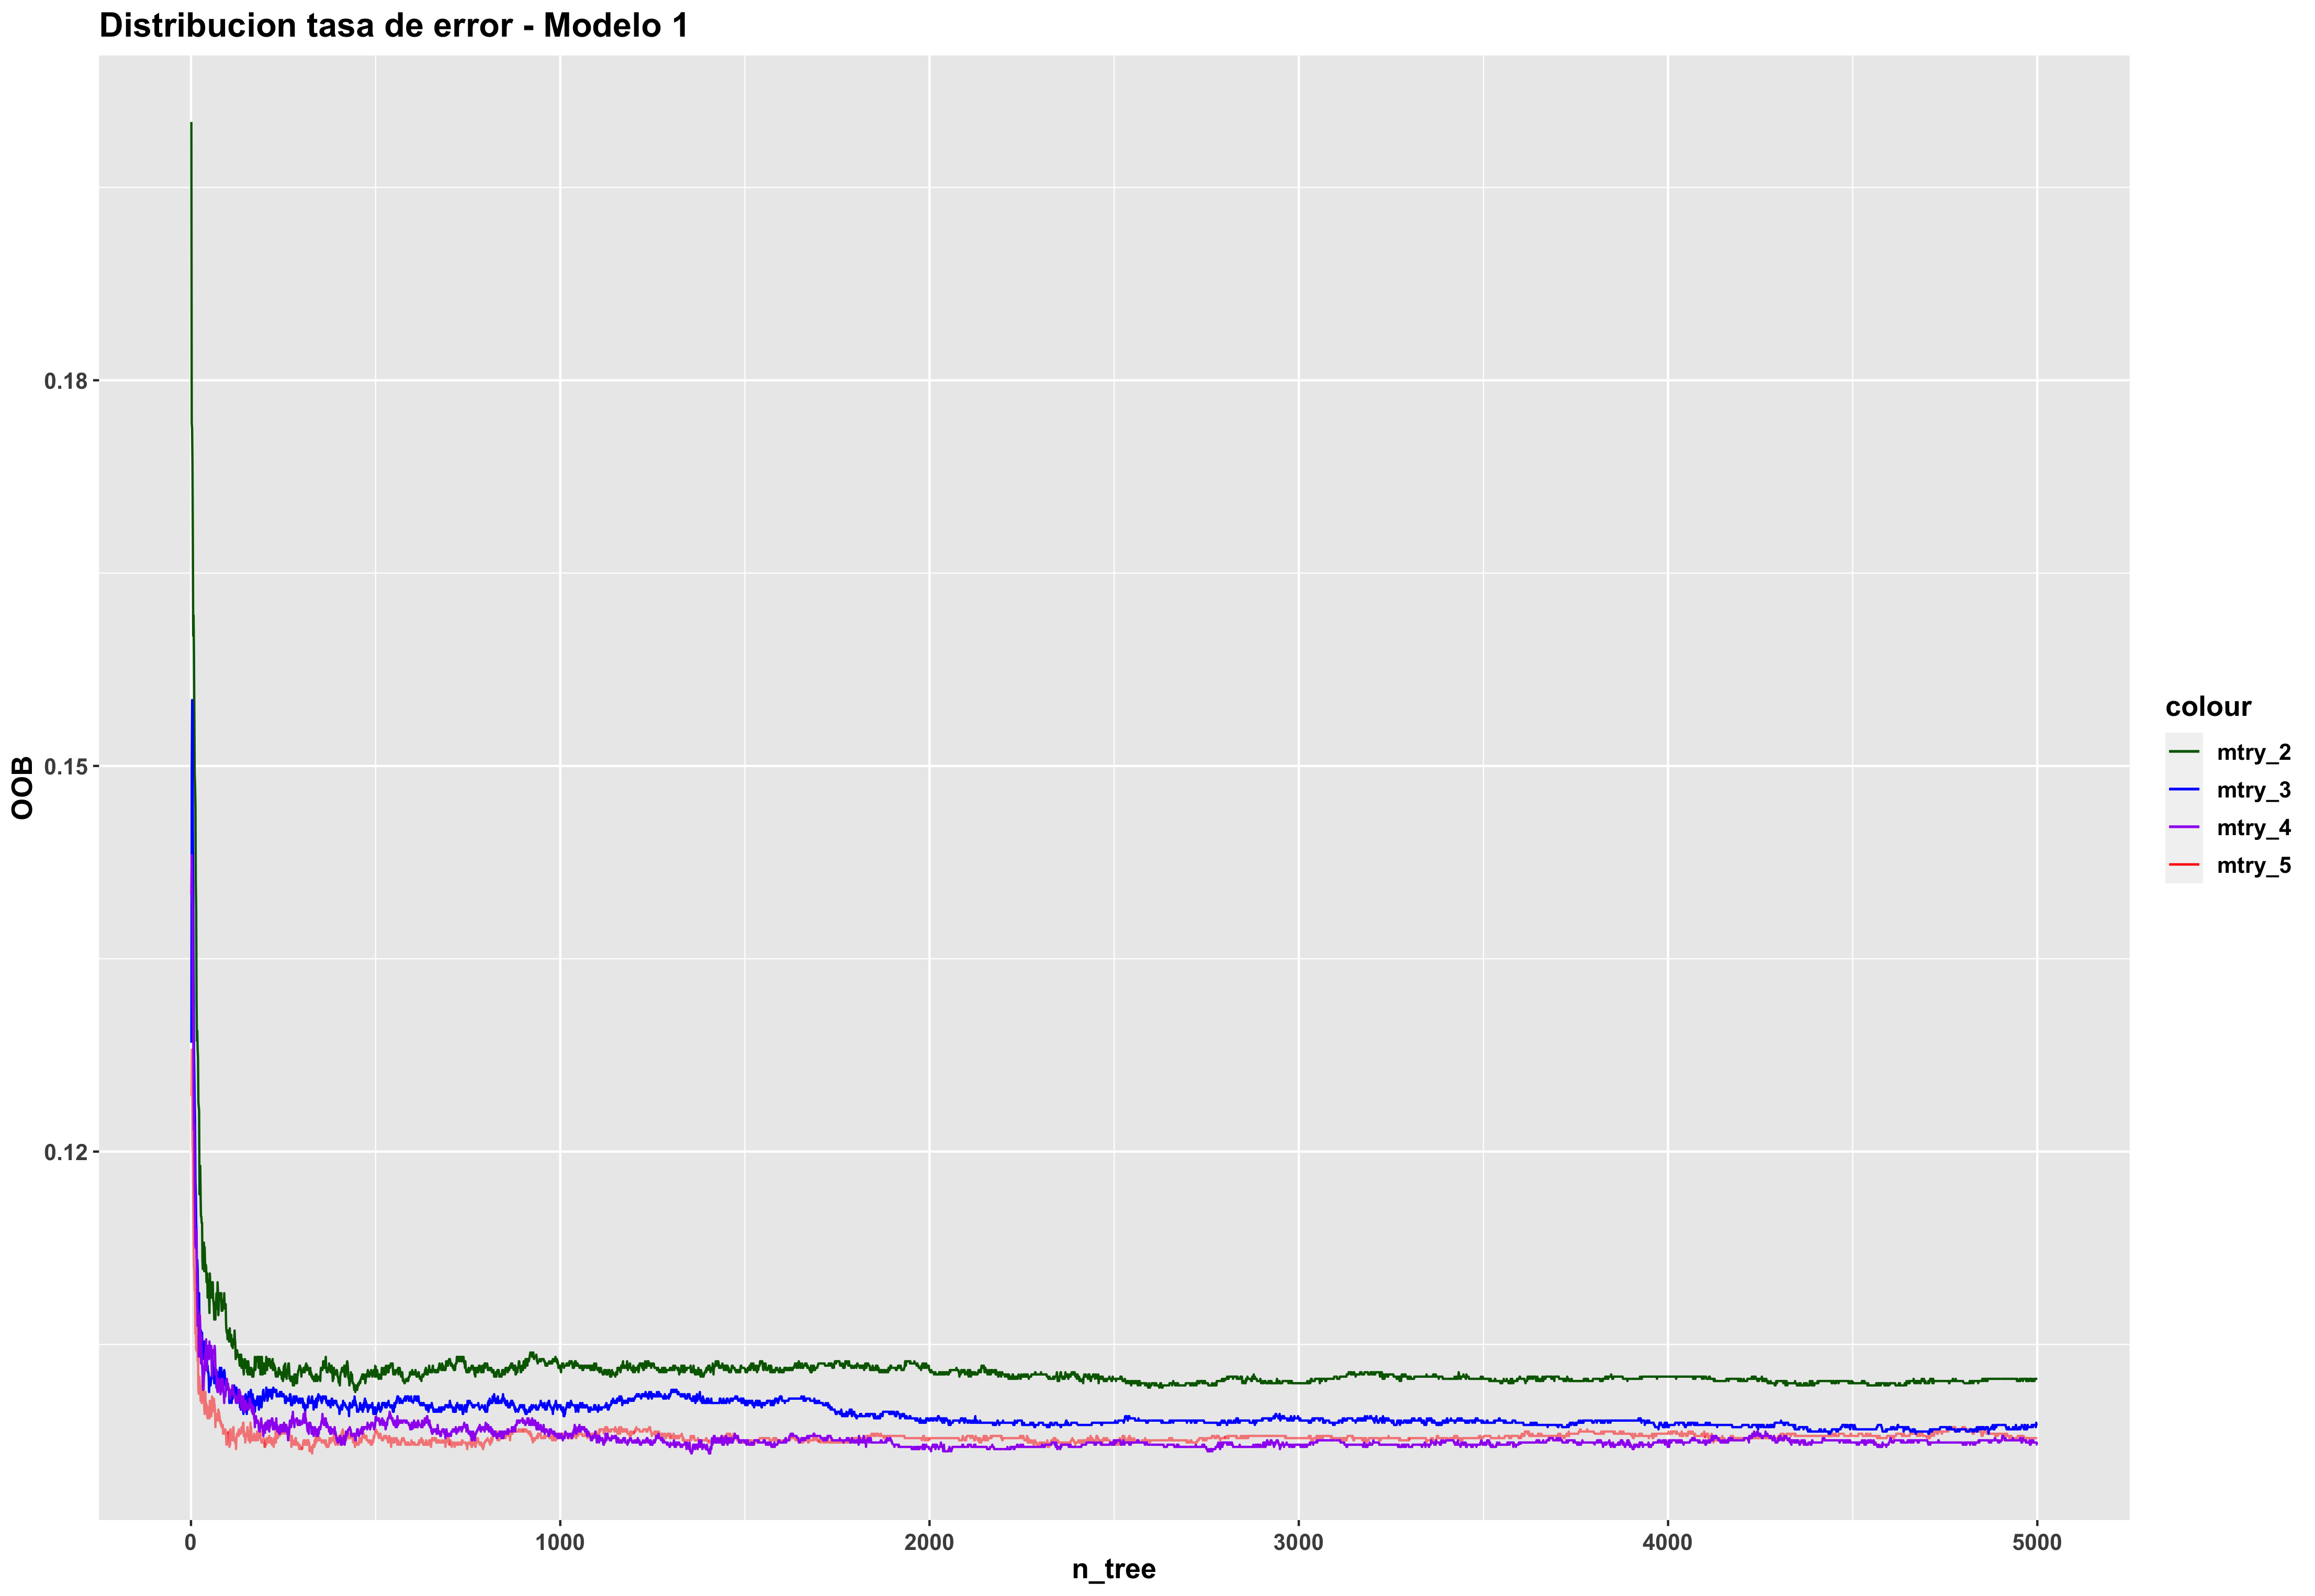
\includegraphics[width=0.99\linewidth,height=0.99\textheight,]{./charts/random_forest/error_rates/error_rate_1} 

}

\caption{Error rate (Modelo 1) en función de mtry}\label{fig:unnamed-chunk-85}
\end{figure}

En primera instancia, observamos que el error (para cualquier
\emph{mtry}) se estabiliza prácticamente a partir de 2000 árboles,
momento en el que el error \emph{Out of bag} es estable con \emph{mtry}
= 2. Sin embargo, con otros valores \emph{mtry}, es decir,
\textbf{sorteando un mayor número de variables}, el error se estabiliza
con antelación:

\begin{enumerate}
\def\labelenumi{\arabic{enumi}.}
\tightlist
\item
  \emph{mtry} = 3: también a partir de 2000 árboles, aproximadamente.
\item
  \emph{mtry} = 4: a partir de 1500 árboles, aproximadamente.
\item
  \emph{mtry} = 5: a partir de 900 árboles (caso del modelo
  \emph{bagging}).
\end{enumerate}

Tras una primera impresión, y utilizando 2000 árboles, \textbf{lanzamos
los primeros modelos \emph{random forest}}, utilizando los diferentes
valores \emph{mtry}. En relación con el resto de parámetros como
\emph{nodesize} o \emph{sampsize}, \textbf{utilizamos los empleados en
el modelo \emph{bagging}}: 20 + 1000.

\begin{Shaded}
\begin{Highlighting}[]
\CommentTok{\#{-}{-} 2500: numero de arboles a partir del cual se estabiliza con mtry = 2}
\CommentTok{\#   Inicialmente, probamos con 5 repeticiones}
\NormalTok{mtry}\FloatTok{.1}\NormalTok{ <{-}}\StringTok{ }\KeywordTok{c}\NormalTok{(}\DecValTok{2}\NormalTok{,}\DecValTok{3}\NormalTok{,}\DecValTok{4}\NormalTok{,}\DecValTok{5}\NormalTok{) }\CommentTok{\# mtry = 5 {-}> modelo bagging}
\NormalTok{primera.imp <{-}}\StringTok{ }\KeywordTok{tuneo\_rf}\NormalTok{(surgical\_dataset, }\DataTypeTok{target=}\NormalTok{target,}\DataTypeTok{lista.continua=}\NormalTok{var\_modelo1,}
                        \DataTypeTok{grupos=}\DecValTok{5}\NormalTok{,}\DataTypeTok{repe=}\DecValTok{5}\NormalTok{,}\DataTypeTok{nodesizes=}\DecValTok{20}\NormalTok{,}\DataTypeTok{mtry=}\NormalTok{mtry}\FloatTok{.1}\NormalTok{,}\DataTypeTok{ntree=}\DecValTok{2000}\NormalTok{,}\DataTypeTok{replace=}\OtherTok{TRUE}\NormalTok{, }
                        \DataTypeTok{sampsizes=}\DecValTok{1000}\NormalTok{)}
\end{Highlighting}
\end{Shaded}

\begin{figure}[h!]

{\centering 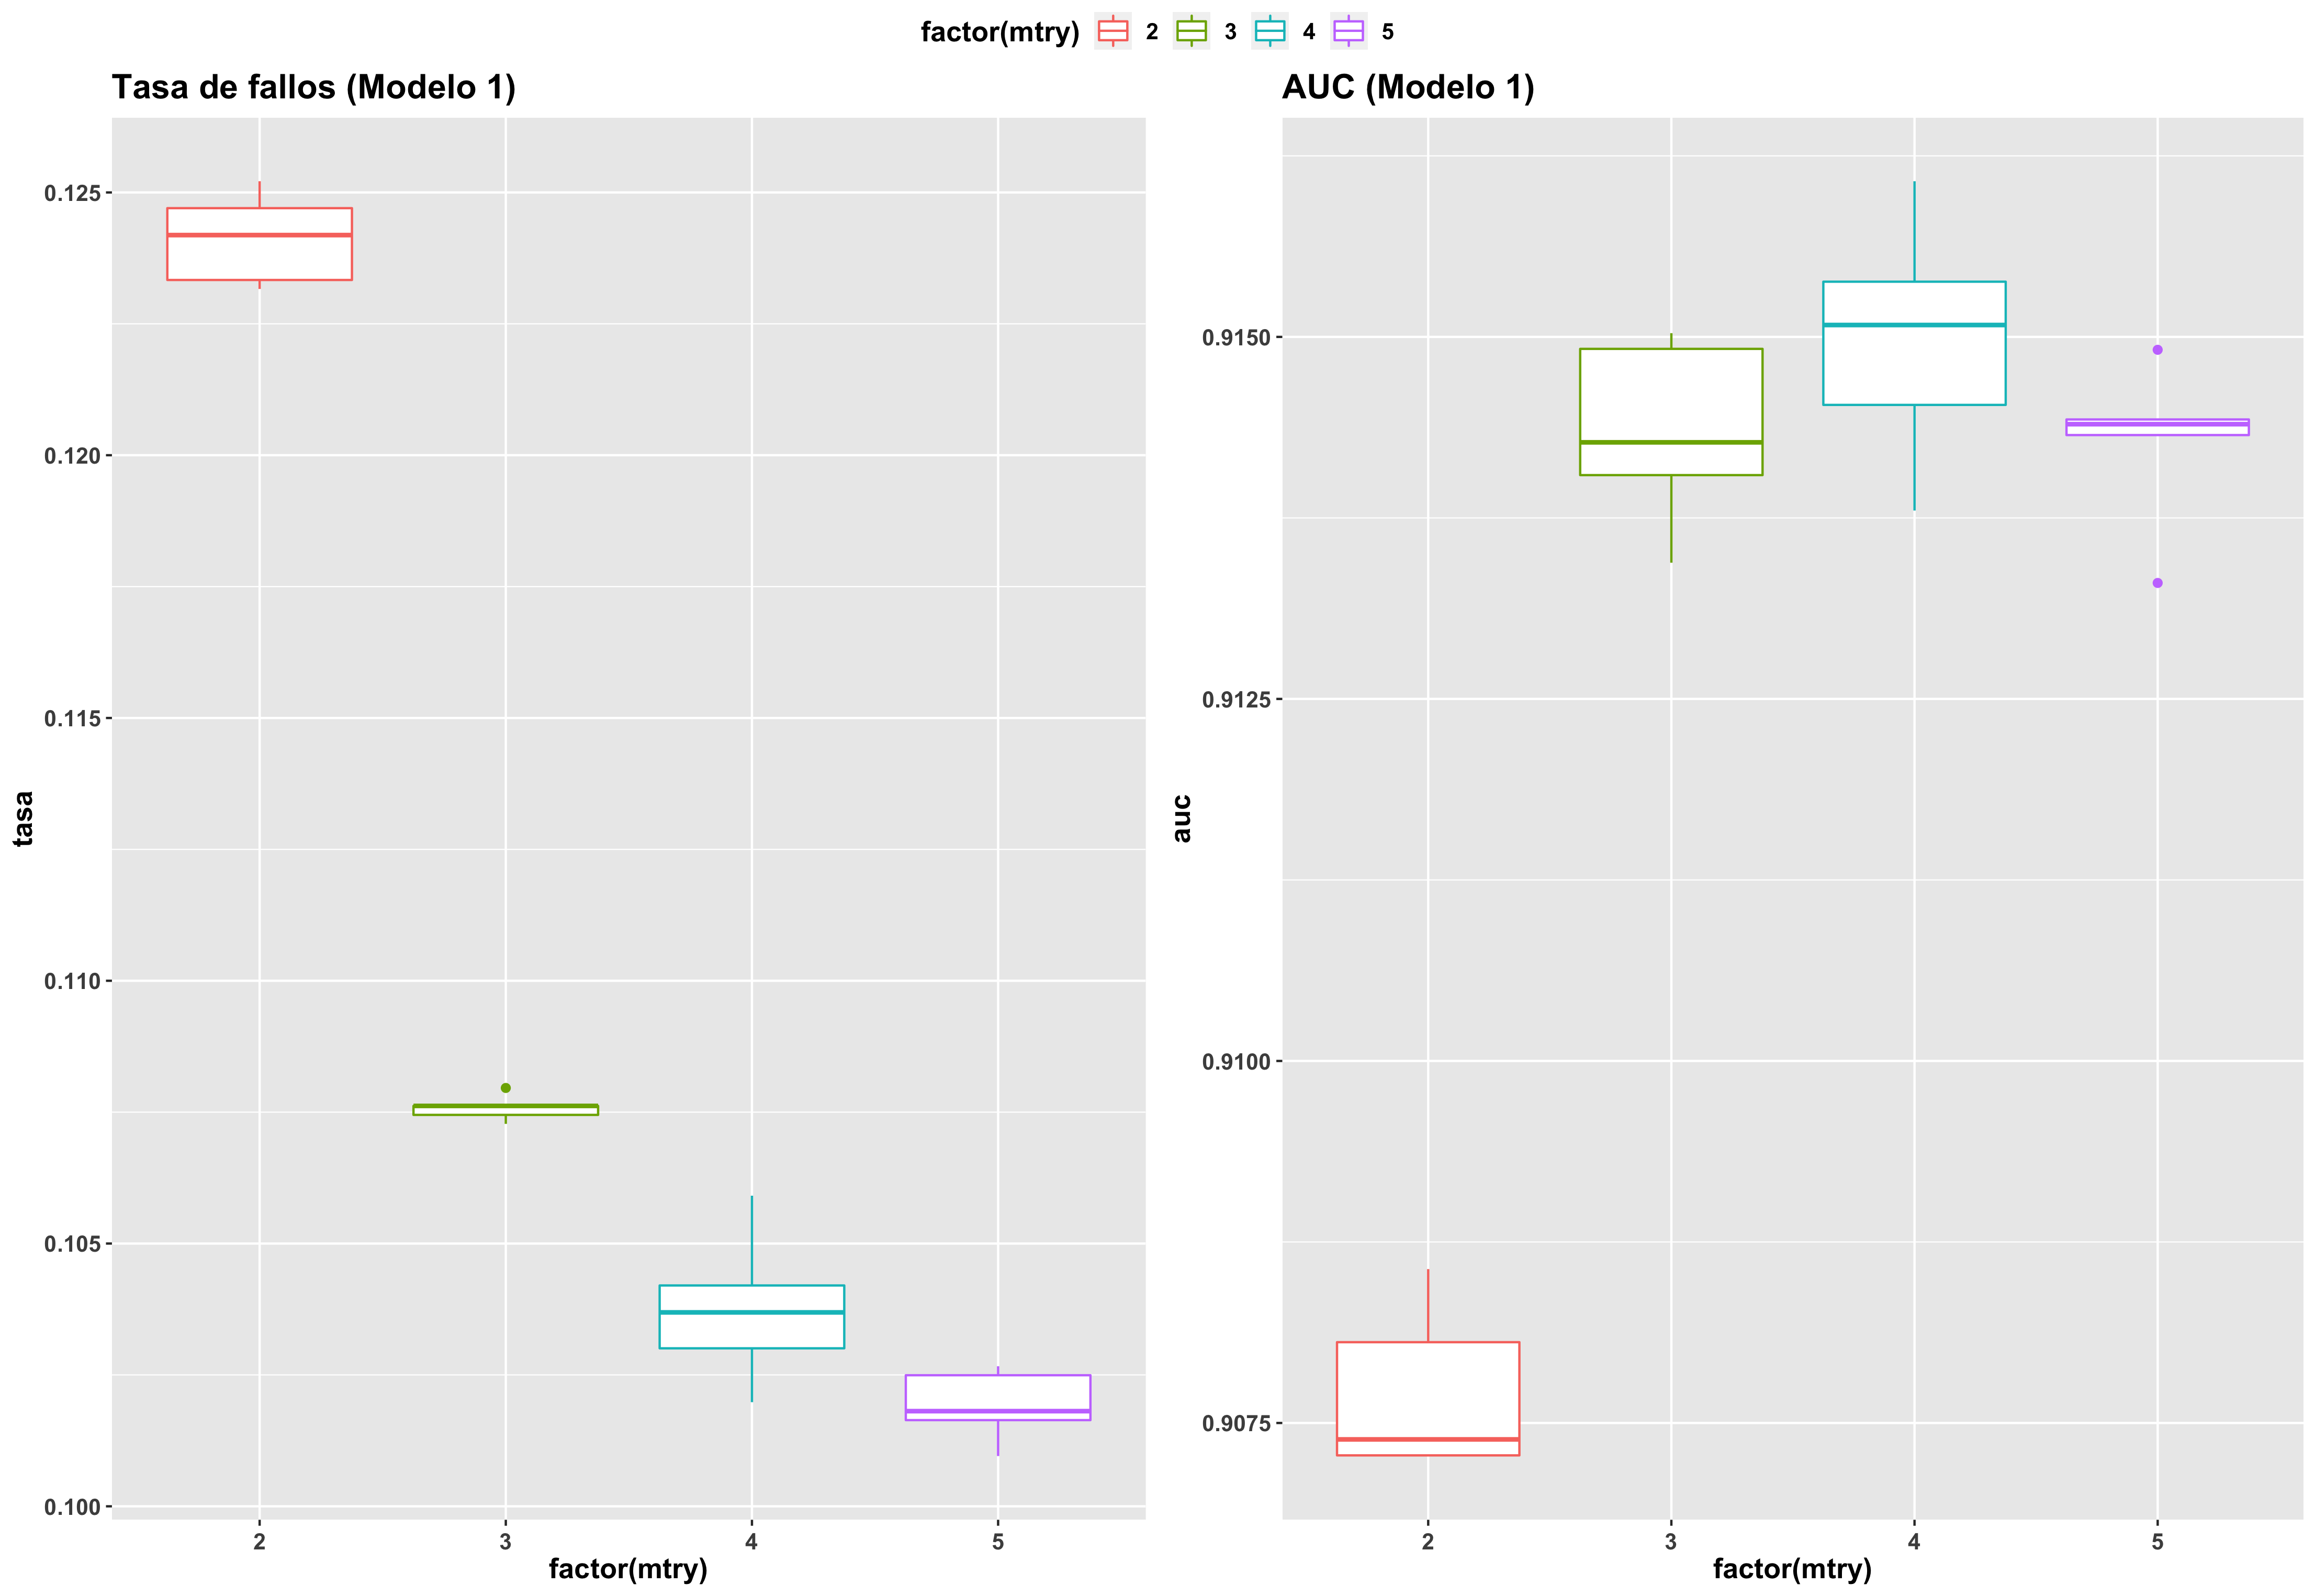
\includegraphics[width=0.99\linewidth,height=0.99\textheight,]{./charts/random_forest/04_comp_inicial_mtry_modelo1} 

}

\caption{Tasa de fallos y AUC en funcion de mtry - Modelo 1}\label{fig:unnamed-chunk-87}
\end{figure}

A simple vista, \textbf{podemos comprobar que no es realmente necesario
sortear todas las variables en cada nivel del árbol, sino que con un
tamaño menor, moderado, en torno a 3, se obtienen los mismos resultados,
aunque con una ganancia en la tasa de fallos muy pequeña} (0.107-0.108
frente a 0.102 del modelo \emph{bagging}). Bien es cierto que con un
\emph{mtry} = 2, la tasa de fallos aumenta (aunque no demasiado) hasta
0.12. Por tanto, y como primera impresión, \textbf{nos decantamos por un
valor \emph{mtry} moderado (3), pero sin llegar a utilizar todas las
variables}.

\hypertarget{modelo-2-1}{%
\subsubsection{8.1.2 Modelo 2}\label{modelo-2-1}}

Del mismo modo, realizamos los mismos pasos para el segundo \emph{set}
candidato, comenzando con el número de árboles:

\begin{figure}[h!]

{\centering 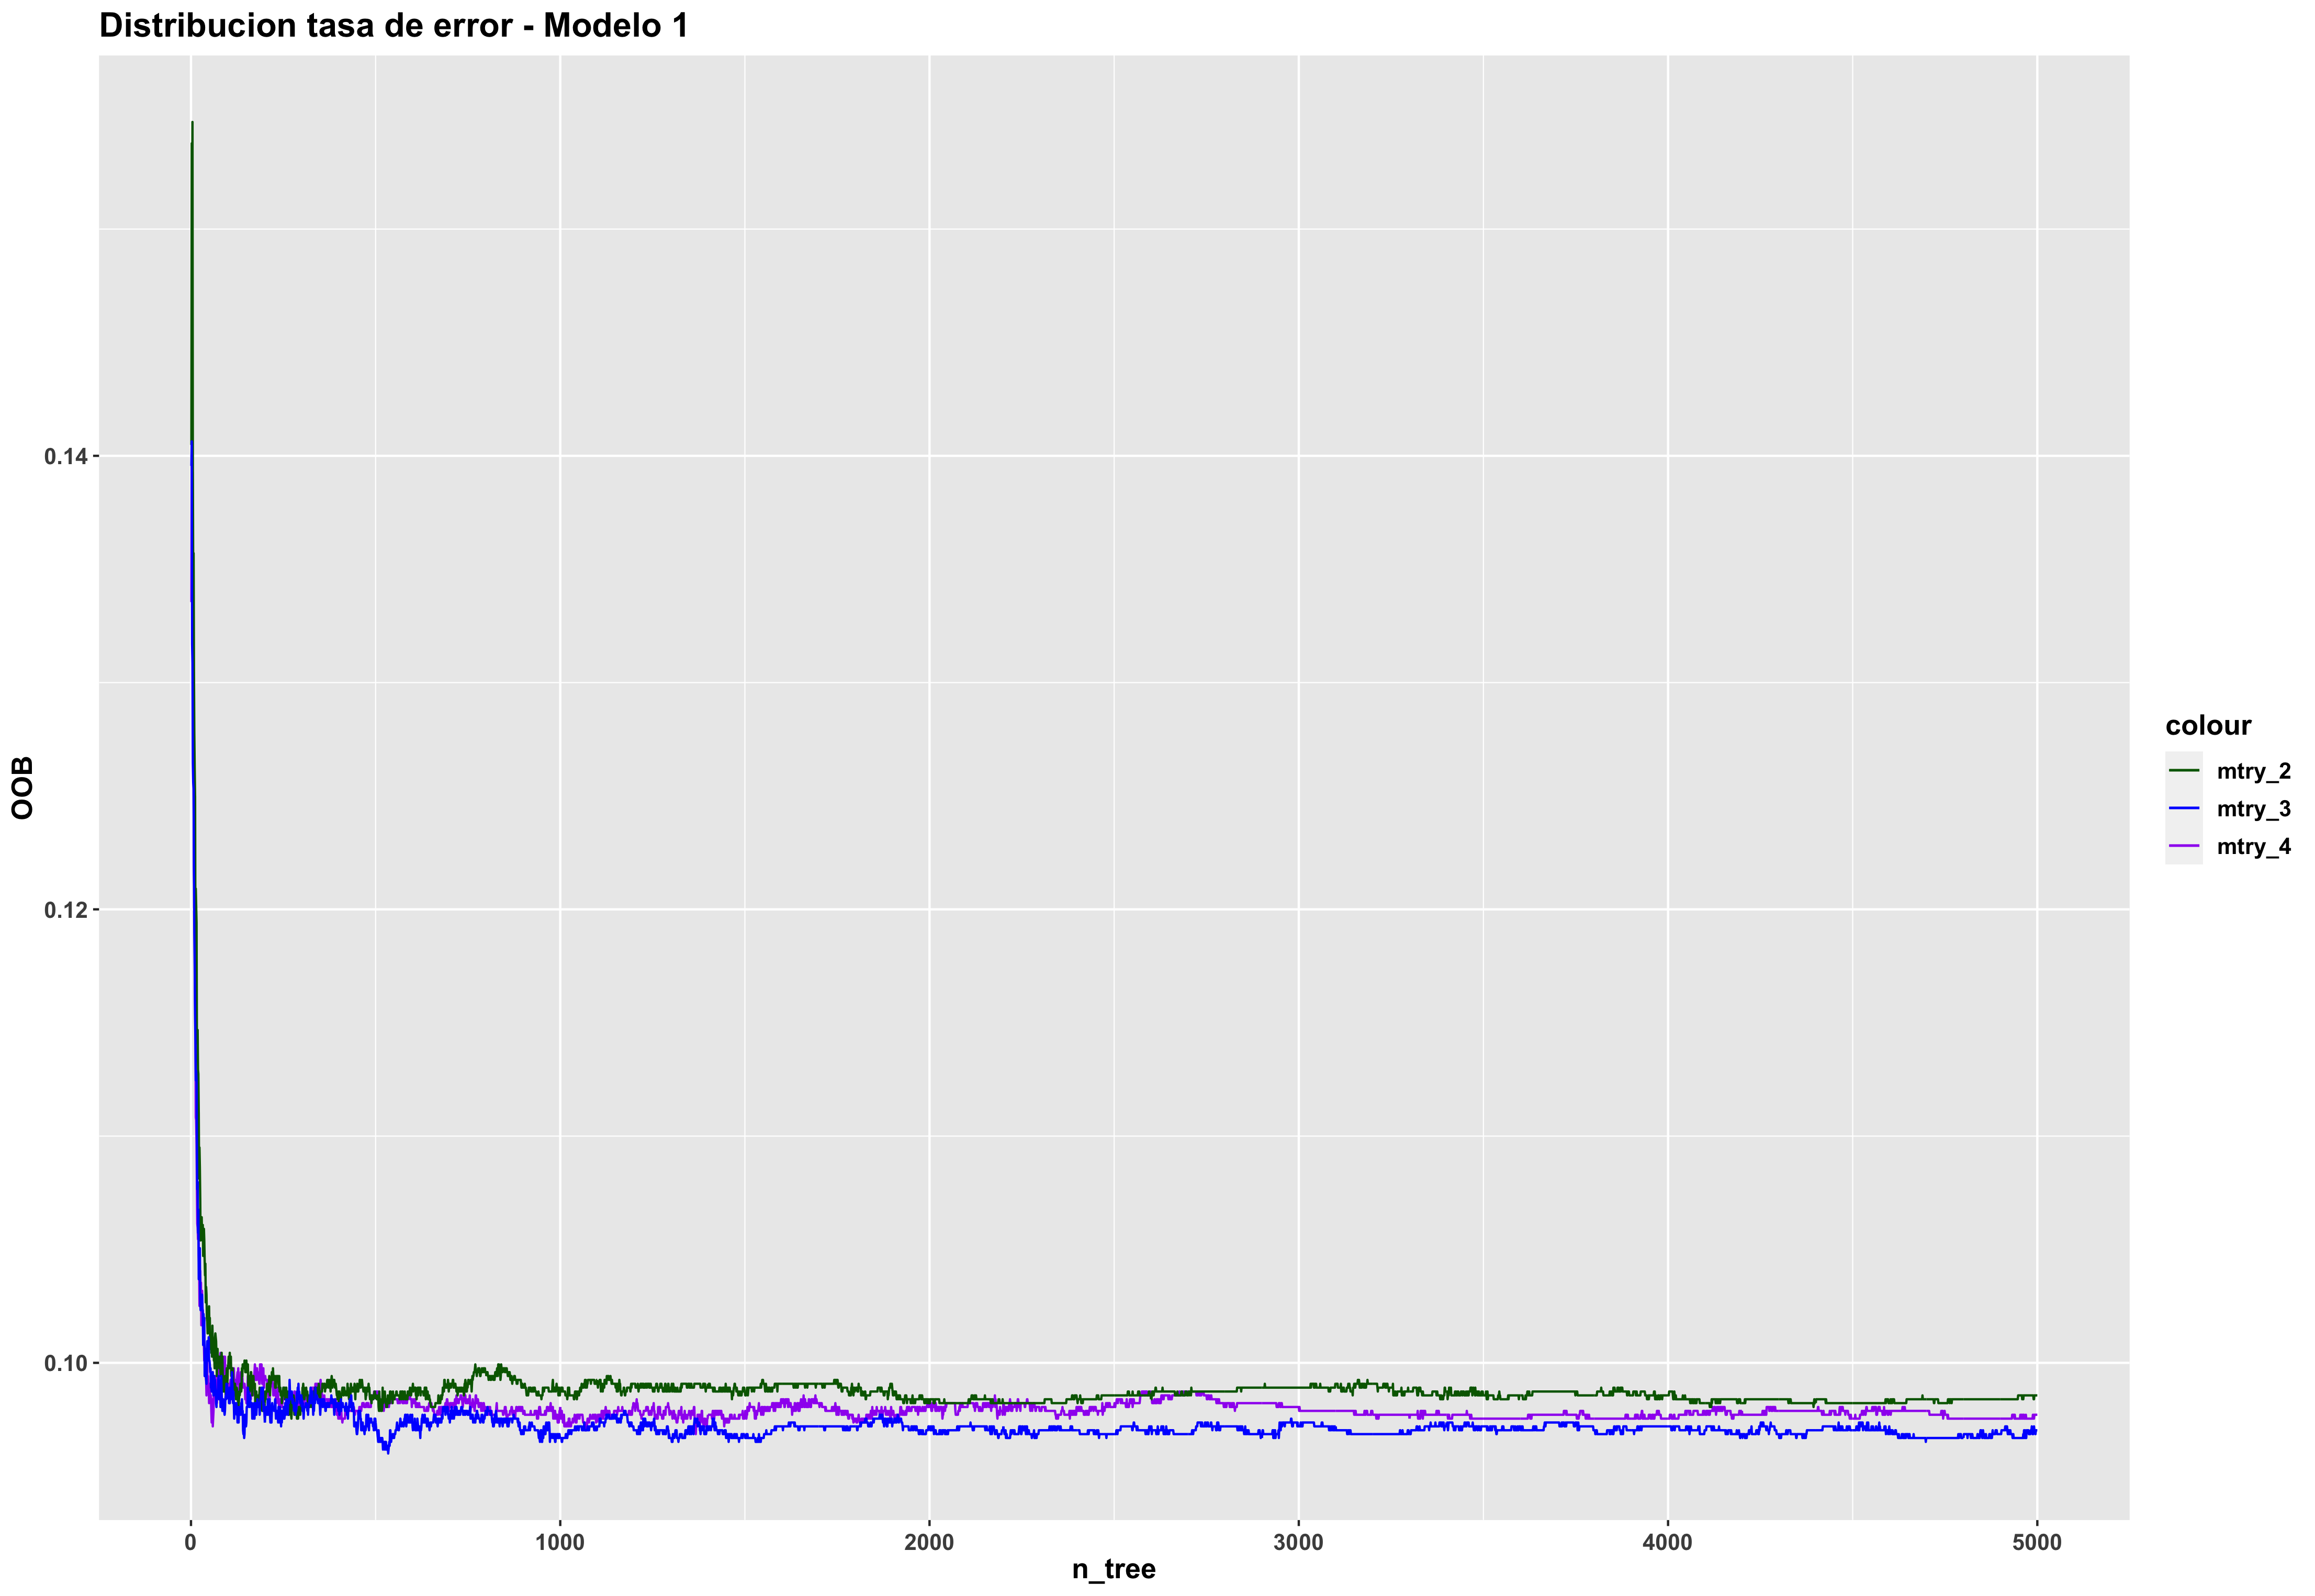
\includegraphics[width=0.99\linewidth,height=0.99\textheight,]{./charts/random_forest/error_rates/error_rate_2} 

}

\caption{Error rate (Modelo 2) en función de mtry}\label{fig:unnamed-chunk-88}
\end{figure}

Al igual que en el primer modelo, a excepción de \emph{mtry} = 4
(correspondiente con un modelo \emph{bagging}), para estabilizar el
error \textbf{se requieren un mayor número de árboles}, en torno a 2000
aproximadamente tanto para \emph{mtry} = 2 como \emph{mtry} = 3. A
continuación, echemos un primer vistazo al comportamiento de los
modelos, tanto en sesgo como en varianza, utilizando los diferentes
valores \emph{mtry}, así como 2000 árboles y el mejor valor \emph{mtry}
y \emph{nodesize} obtenidos en \emph{bagging} para el segundo \emph{set}
de variables (20 + 1000):

\begin{figure}[h!]

{\centering 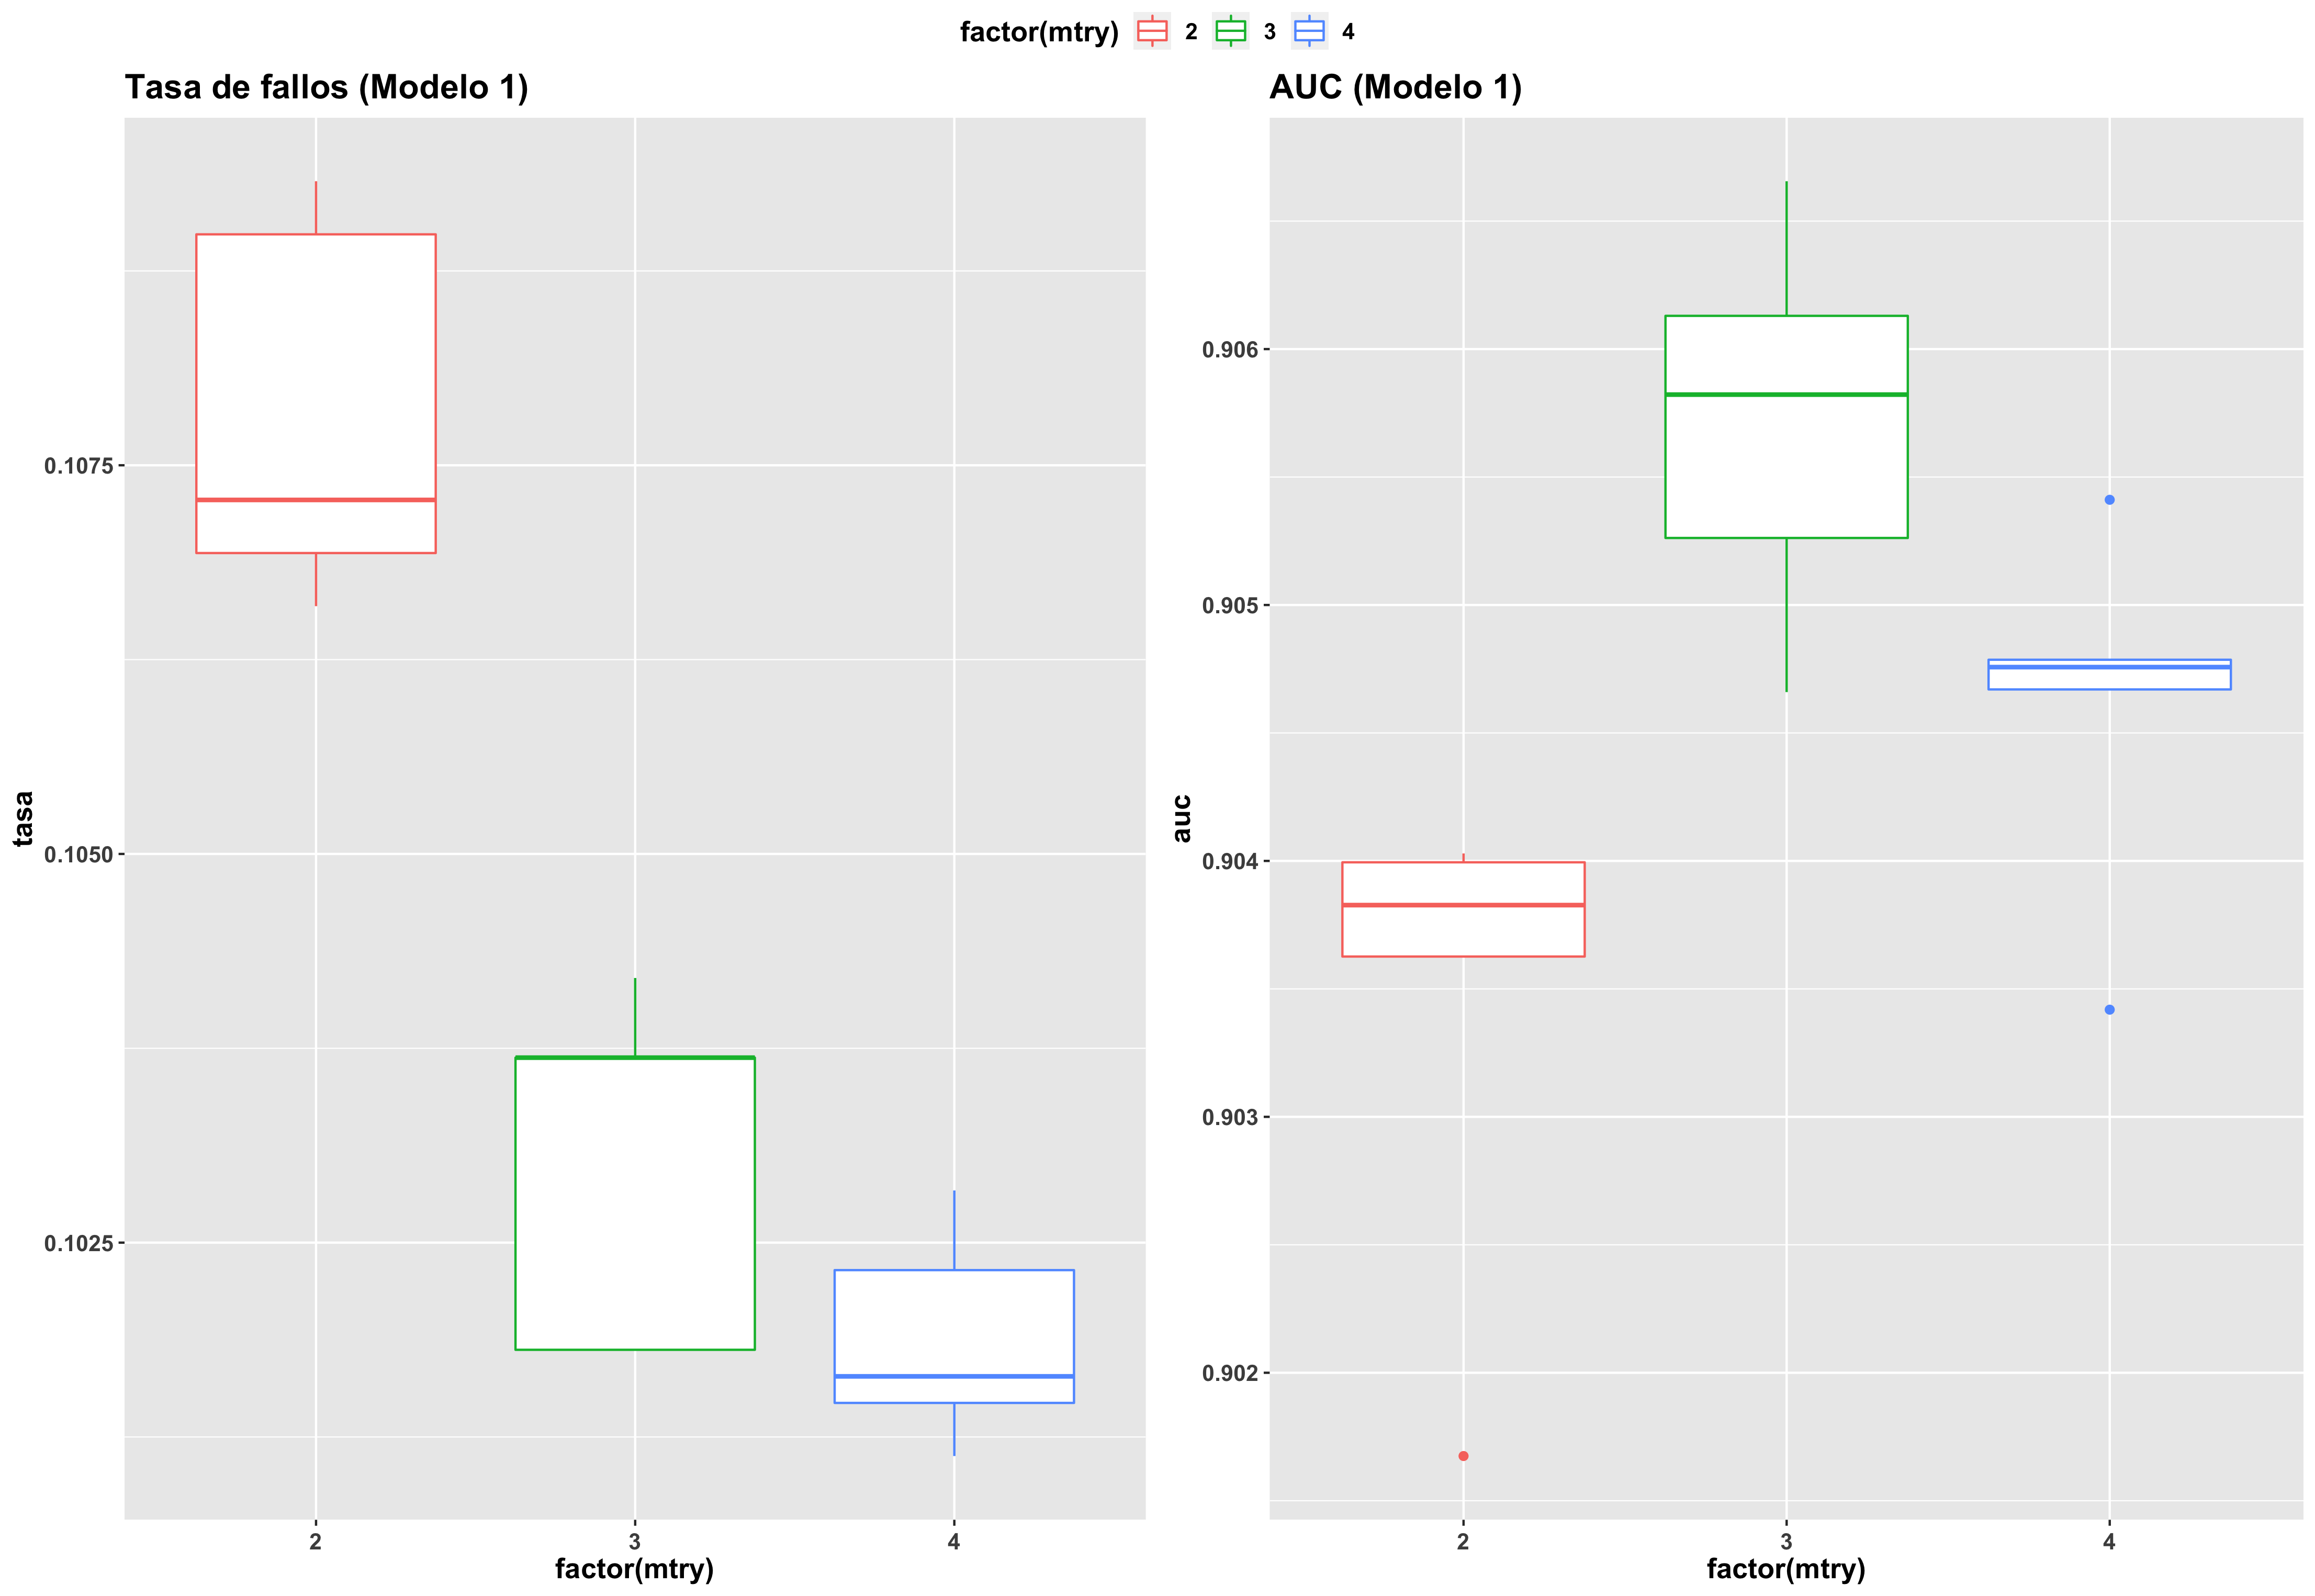
\includegraphics[width=0.99\linewidth,height=0.99\textheight,]{./charts/random_forest/04_comp_inicial_mtry_modelo2} 

}

\caption{Tasa de fallos y AUC en funcion de mtry - Modelo 2}\label{fig:unnamed-chunk-89}
\end{figure}

En primera instancia, una posibilidad sería decantarse por un modelo con
\emph{mtry} = 3, sin llegar a utilizar todas las variables. Sin embargo,
y en base a la escala del eje Y, \textbf{el error y varianza que
presenta el modelo con \emph{mtry} = 2 no es tan pronunciado}:

\begin{enumerate}
\def\labelenumi{\arabic{enumi}.}
\item
  En el caso de la tasa de fallos, la diferencia es 0.005 (de 0.1025 en
  el caso de \emph{mtry} = 4 a 0.1075 en el caso de \emph{mtry} = 2).
  Además, la varianza que presenta en torno al modelo, teniendo en
  cuenta la escala del eje, es del orden de milésimas.
\item
  En el caso del área bajo la curva ROC, la diferencia también se sitúa
  en torno a las milésimas (de 0.906 en el caso de \emph{mtry} = 4 a
  0.904 en el caso de \emph{mtry} = 2).
\end{enumerate}

Dicha diferencia puede ser debida a numerosos factores: estructura de
remuestreo, selección de observaciones con \emph{sampsize}, valor de la
semilla etc. Por tanto, dado que la diferencia no es apenas relevante,
con el segundo \emph{set} de variables \textbf{nos decantamos por un
valor \emph{mtry} = 2}.

\hypertarget{modelo-1-2}{%
\subsection{8.2 Modelo 1}\label{modelo-1-2}}

En un primer comienzo, con un valor \emph{mtry} = 3 y el mismo
\emph{nodesize} y \emph{sampsize} que en el modelo \emph{bagging},
obtenemos muy buenos resultados. No obstante, hemos considera un valor
de \emph{nodesize} y \emph{sampsize} por defecto, esto es, los mejores
parámetros obtenidos en \emph{bagging}. Por tanto, ¿Puede llegar a ser
influyente el hecho de aumentar o reducir el valor \emph{nodesize}, o
más importante aún, el tamaño de la submuestra en \emph{sampsize}? Del
mismo modo que en \emph{bagging}, analicemos la importancia de ambos
parámetros, tuneando el modelo con diferentes valores (comenzando con
tan solo 5 repeticiones):

\begin{Shaded}
\begin{Highlighting}[]
\NormalTok{sampsizes}\FloatTok{.1}\NormalTok{ <{-}}\StringTok{ }\KeywordTok{list}\NormalTok{(}\DecValTok{1}\NormalTok{, }\DecValTok{100}\NormalTok{, }\DecValTok{500}\NormalTok{, }\DecValTok{1000}\NormalTok{, }\DecValTok{2000}\NormalTok{, }\DecValTok{3000}\NormalTok{, }\DecValTok{4600}\NormalTok{)}
\NormalTok{nodesizes}\FloatTok{.1}\NormalTok{ <{-}}\StringTok{ }\KeywordTok{list}\NormalTok{(}\DecValTok{5}\NormalTok{, }\DecValTok{10}\NormalTok{, }\DecValTok{20}\NormalTok{, }\DecValTok{30}\NormalTok{, }\DecValTok{40}\NormalTok{, }\DecValTok{50}\NormalTok{, }\DecValTok{100}\NormalTok{)}

\CommentTok{\# Tuneamos nuevamente tanto nodesizes como sampsizes}
\CommentTok{\# sampsize maximo: (4/5) * 5854 \textasciitilde{} 4600 observaciones}
\NormalTok{bagging\_modelo1\_mtry3 <{-}}\StringTok{  }\KeywordTok{tuneo\_rf}\NormalTok{(surgical\_dataset, }\DataTypeTok{target =}\NormalTok{ target,}
                                   \DataTypeTok{lista.continua =}\NormalTok{ var\_modelo1,}
                                   \DataTypeTok{nodesizes =}\NormalTok{ nodesizes}\FloatTok{.1}\NormalTok{,}
                                   \DataTypeTok{sampsizes =}\NormalTok{ sampsizes}\FloatTok{.1}\NormalTok{, }\DataTypeTok{mtry =} \DecValTok{3}\NormalTok{,}
                                   \DataTypeTok{ntree =} \DecValTok{2000}\NormalTok{, }\DataTypeTok{grupos =} \DecValTok{5}\NormalTok{, }\DataTypeTok{repe =} \DecValTok{5}\NormalTok{)}
\end{Highlighting}
\end{Shaded}

\begin{figure}[h!]

{\centering 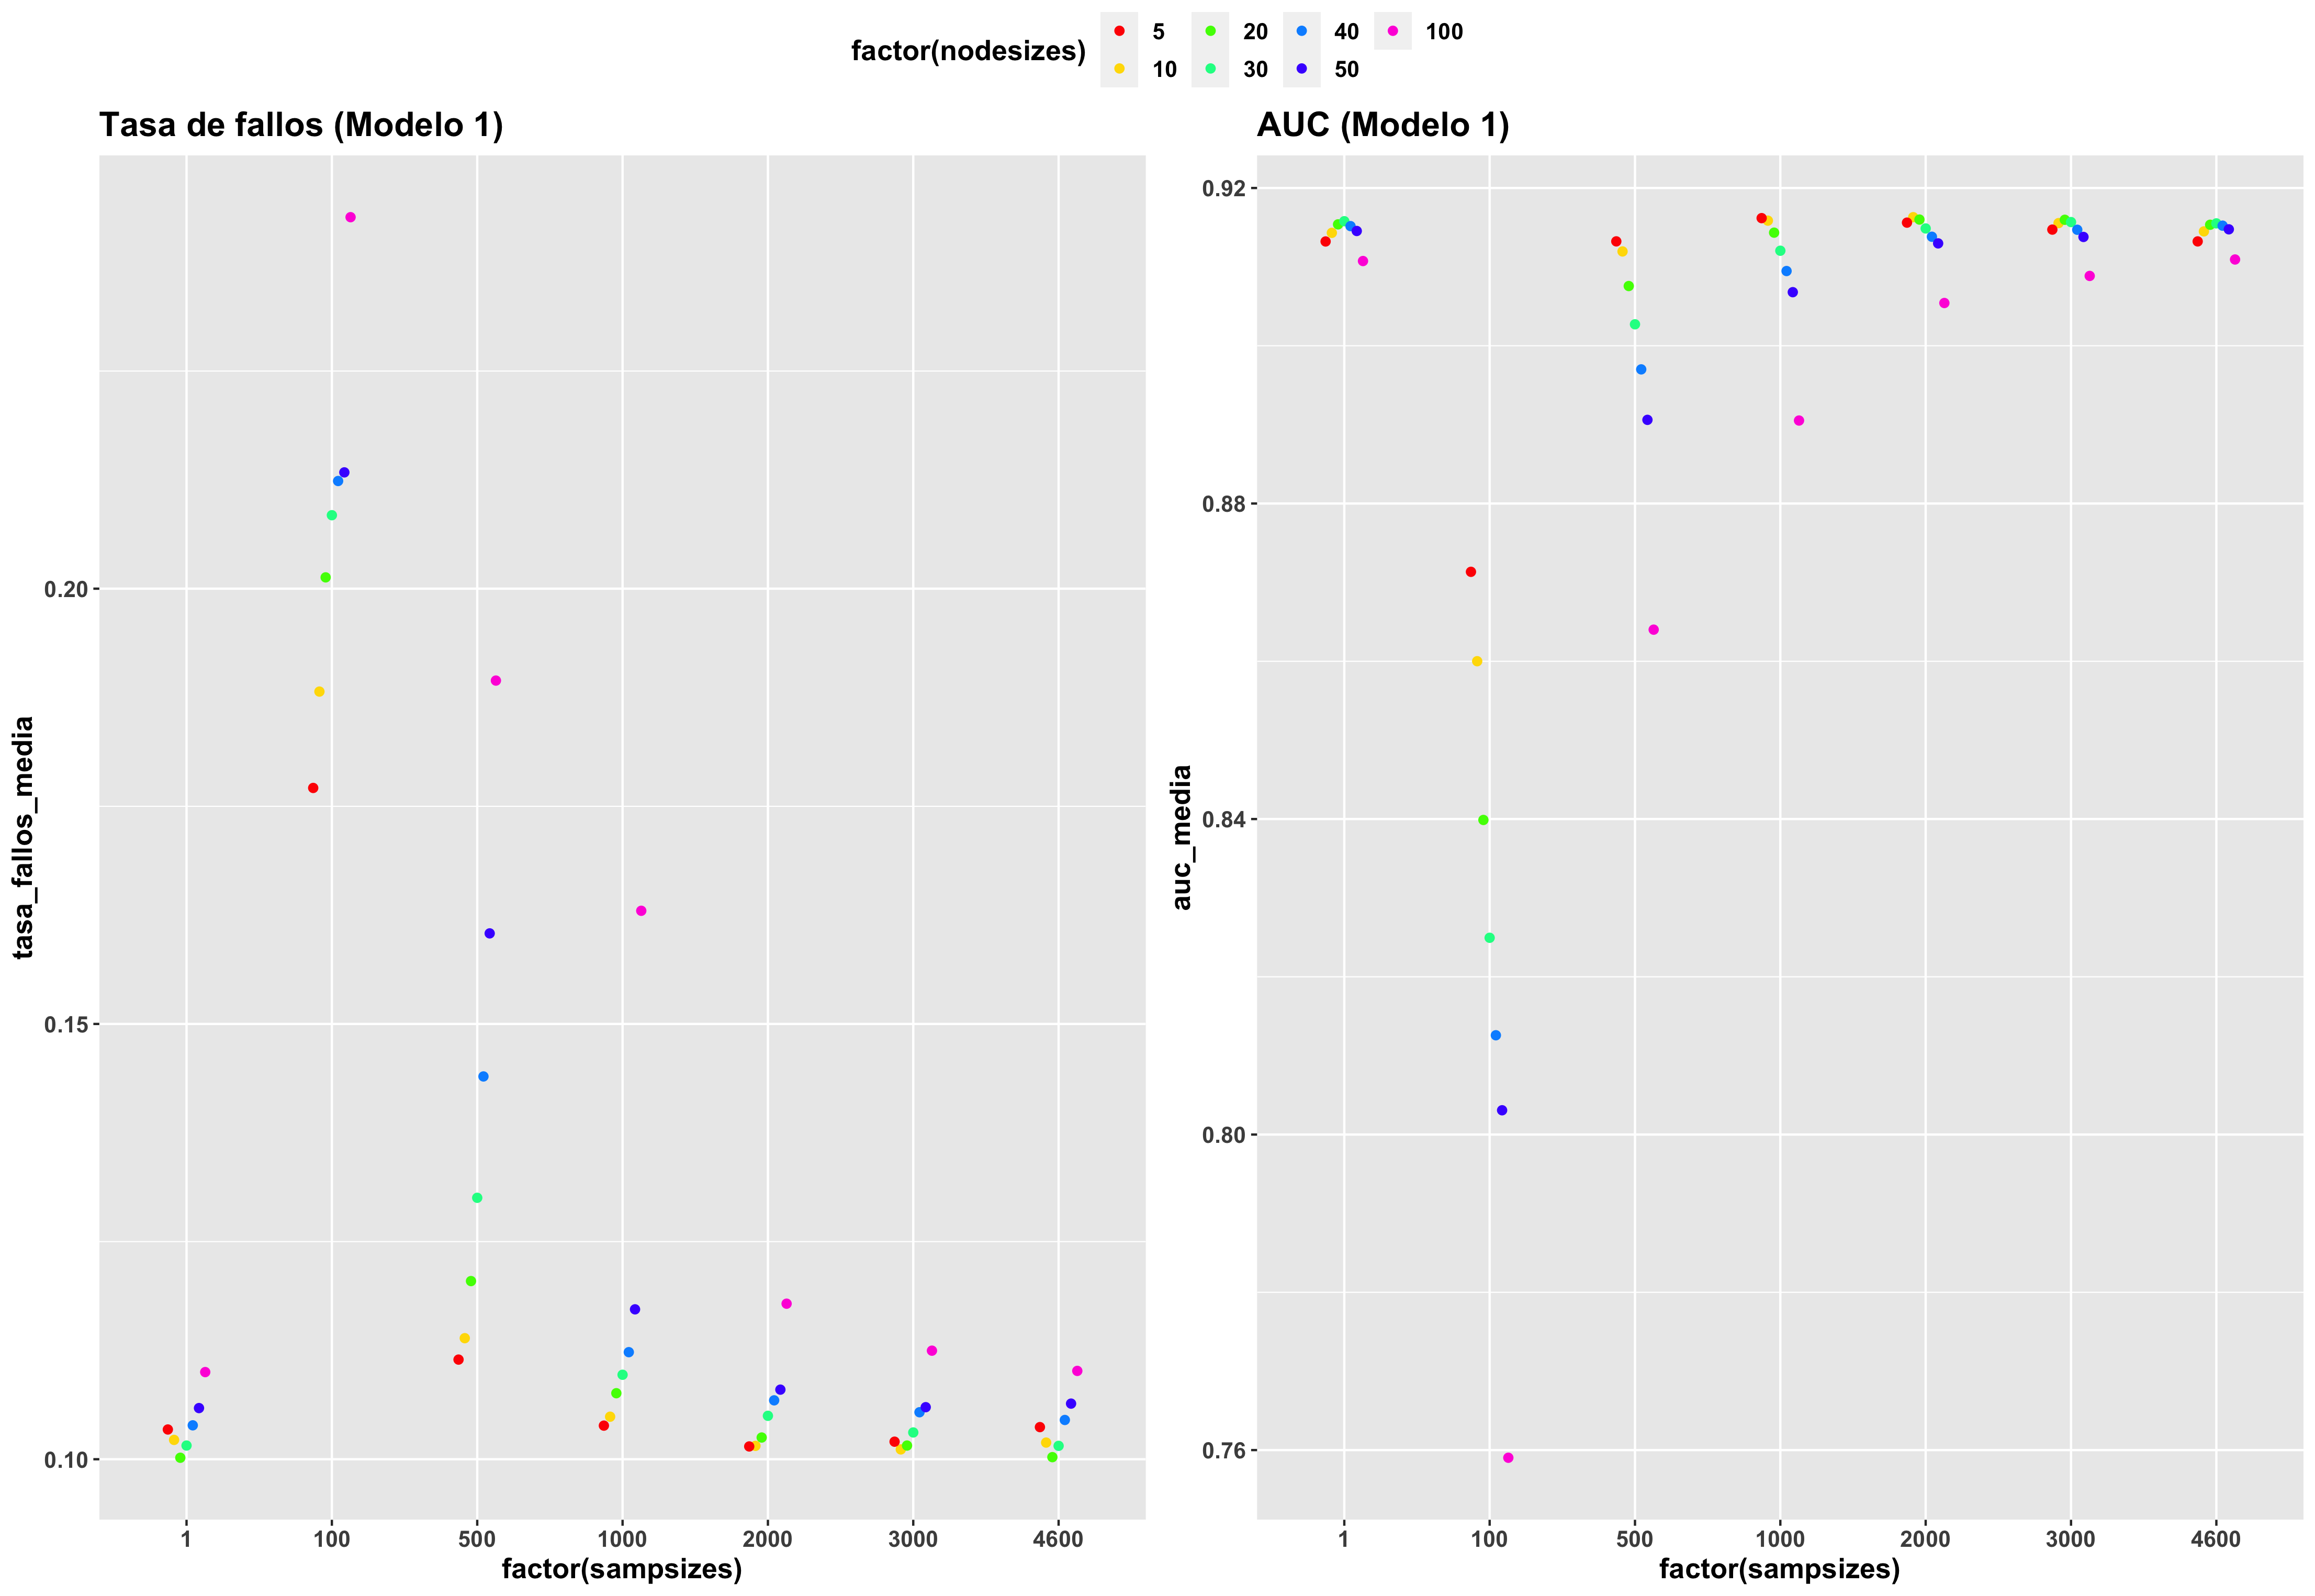
\includegraphics[width=0.99\linewidth,height=0.99\textheight,]{./charts/random_forest/04_comp_tasa_auc_modelo1} 

}

\caption{Tasa de fallos y AUC en funcion de nodesize y sampsize - Modelo 1}\label{fig:unnamed-chunk-91}
\end{figure}

Analizando el promedio de cada modelo, detectamos prácitcamente las
mismas características que en el modelo \emph{bagging}:

\begin{enumerate}
\def\labelenumi{\arabic{enumi}.}
\item
  \textbf{Aumentar la complejidad del árbol, con un \emph{nodesize}
  menor, la ganancia que supone tanto en tasa de fallos como en AUC no
  es muy relevante}, por lo que podemos mantener 20 como tamaño mínimo
  de cada nodo.
\item
  Además, a simple vista \textbf{un valor \emph{sampsize} en torno a
  500-1000 vuelve a ser una buena opción, obteniendo los mismos
  resultados que con el conjunto total de las observaciones}, lo que
  permite la construcción de árboles mucho más diferentes entre si
  gracias al sorteo de menos muestras. No obstante, analicemos más en
  detalle tanto el sesgo como la varianza al variar el tamaño de la
  muestra (manteniendo el valor \emph{nodesize} a 20 y aumentando a el
  número de repeticiones a 10):
\end{enumerate}

\begin{Shaded}
\begin{Highlighting}[]
\NormalTok{nodesizes}\FloatTok{.1}\NormalTok{ <{-}}\StringTok{ }\KeywordTok{list}\NormalTok{(}\DecValTok{20}\NormalTok{)}
\CommentTok{\# Probamos con un tamaño sampsize entre 500 y 3000 (1 = todas las observaciones)}
\NormalTok{sampsizes}\FloatTok{.1}\NormalTok{ <{-}}\StringTok{ }\KeywordTok{list}\NormalTok{(}\DecValTok{1}\NormalTok{, }\DecValTok{500}\NormalTok{, }\DecValTok{1000}\NormalTok{, }\DecValTok{2000}\NormalTok{, }\DecValTok{3000}\NormalTok{)}

\NormalTok{bagging\_modelo1\_mtry3 <{-}}\StringTok{  }\KeywordTok{tuneo\_rf}\NormalTok{(surgical\_dataset, }\DataTypeTok{target =}\NormalTok{ target,}
                                   \DataTypeTok{lista.continua =}\NormalTok{ var\_modelo1,}
                                   \DataTypeTok{nodesizes =}\NormalTok{ nodesizes}\FloatTok{.1}\NormalTok{,}
                                   \DataTypeTok{sampsizes =}\NormalTok{ sampsizes}\FloatTok{.1}\NormalTok{, }\DataTypeTok{mtry =} \DecValTok{3}\NormalTok{,}
                                   \DataTypeTok{ntree =} \DecValTok{2000}\NormalTok{, }\DataTypeTok{grupos =} \DecValTok{5}\NormalTok{, }\DataTypeTok{repe =} \DecValTok{10}\NormalTok{)}
\end{Highlighting}
\end{Shaded}

\begin{figure}[h!]

{\centering 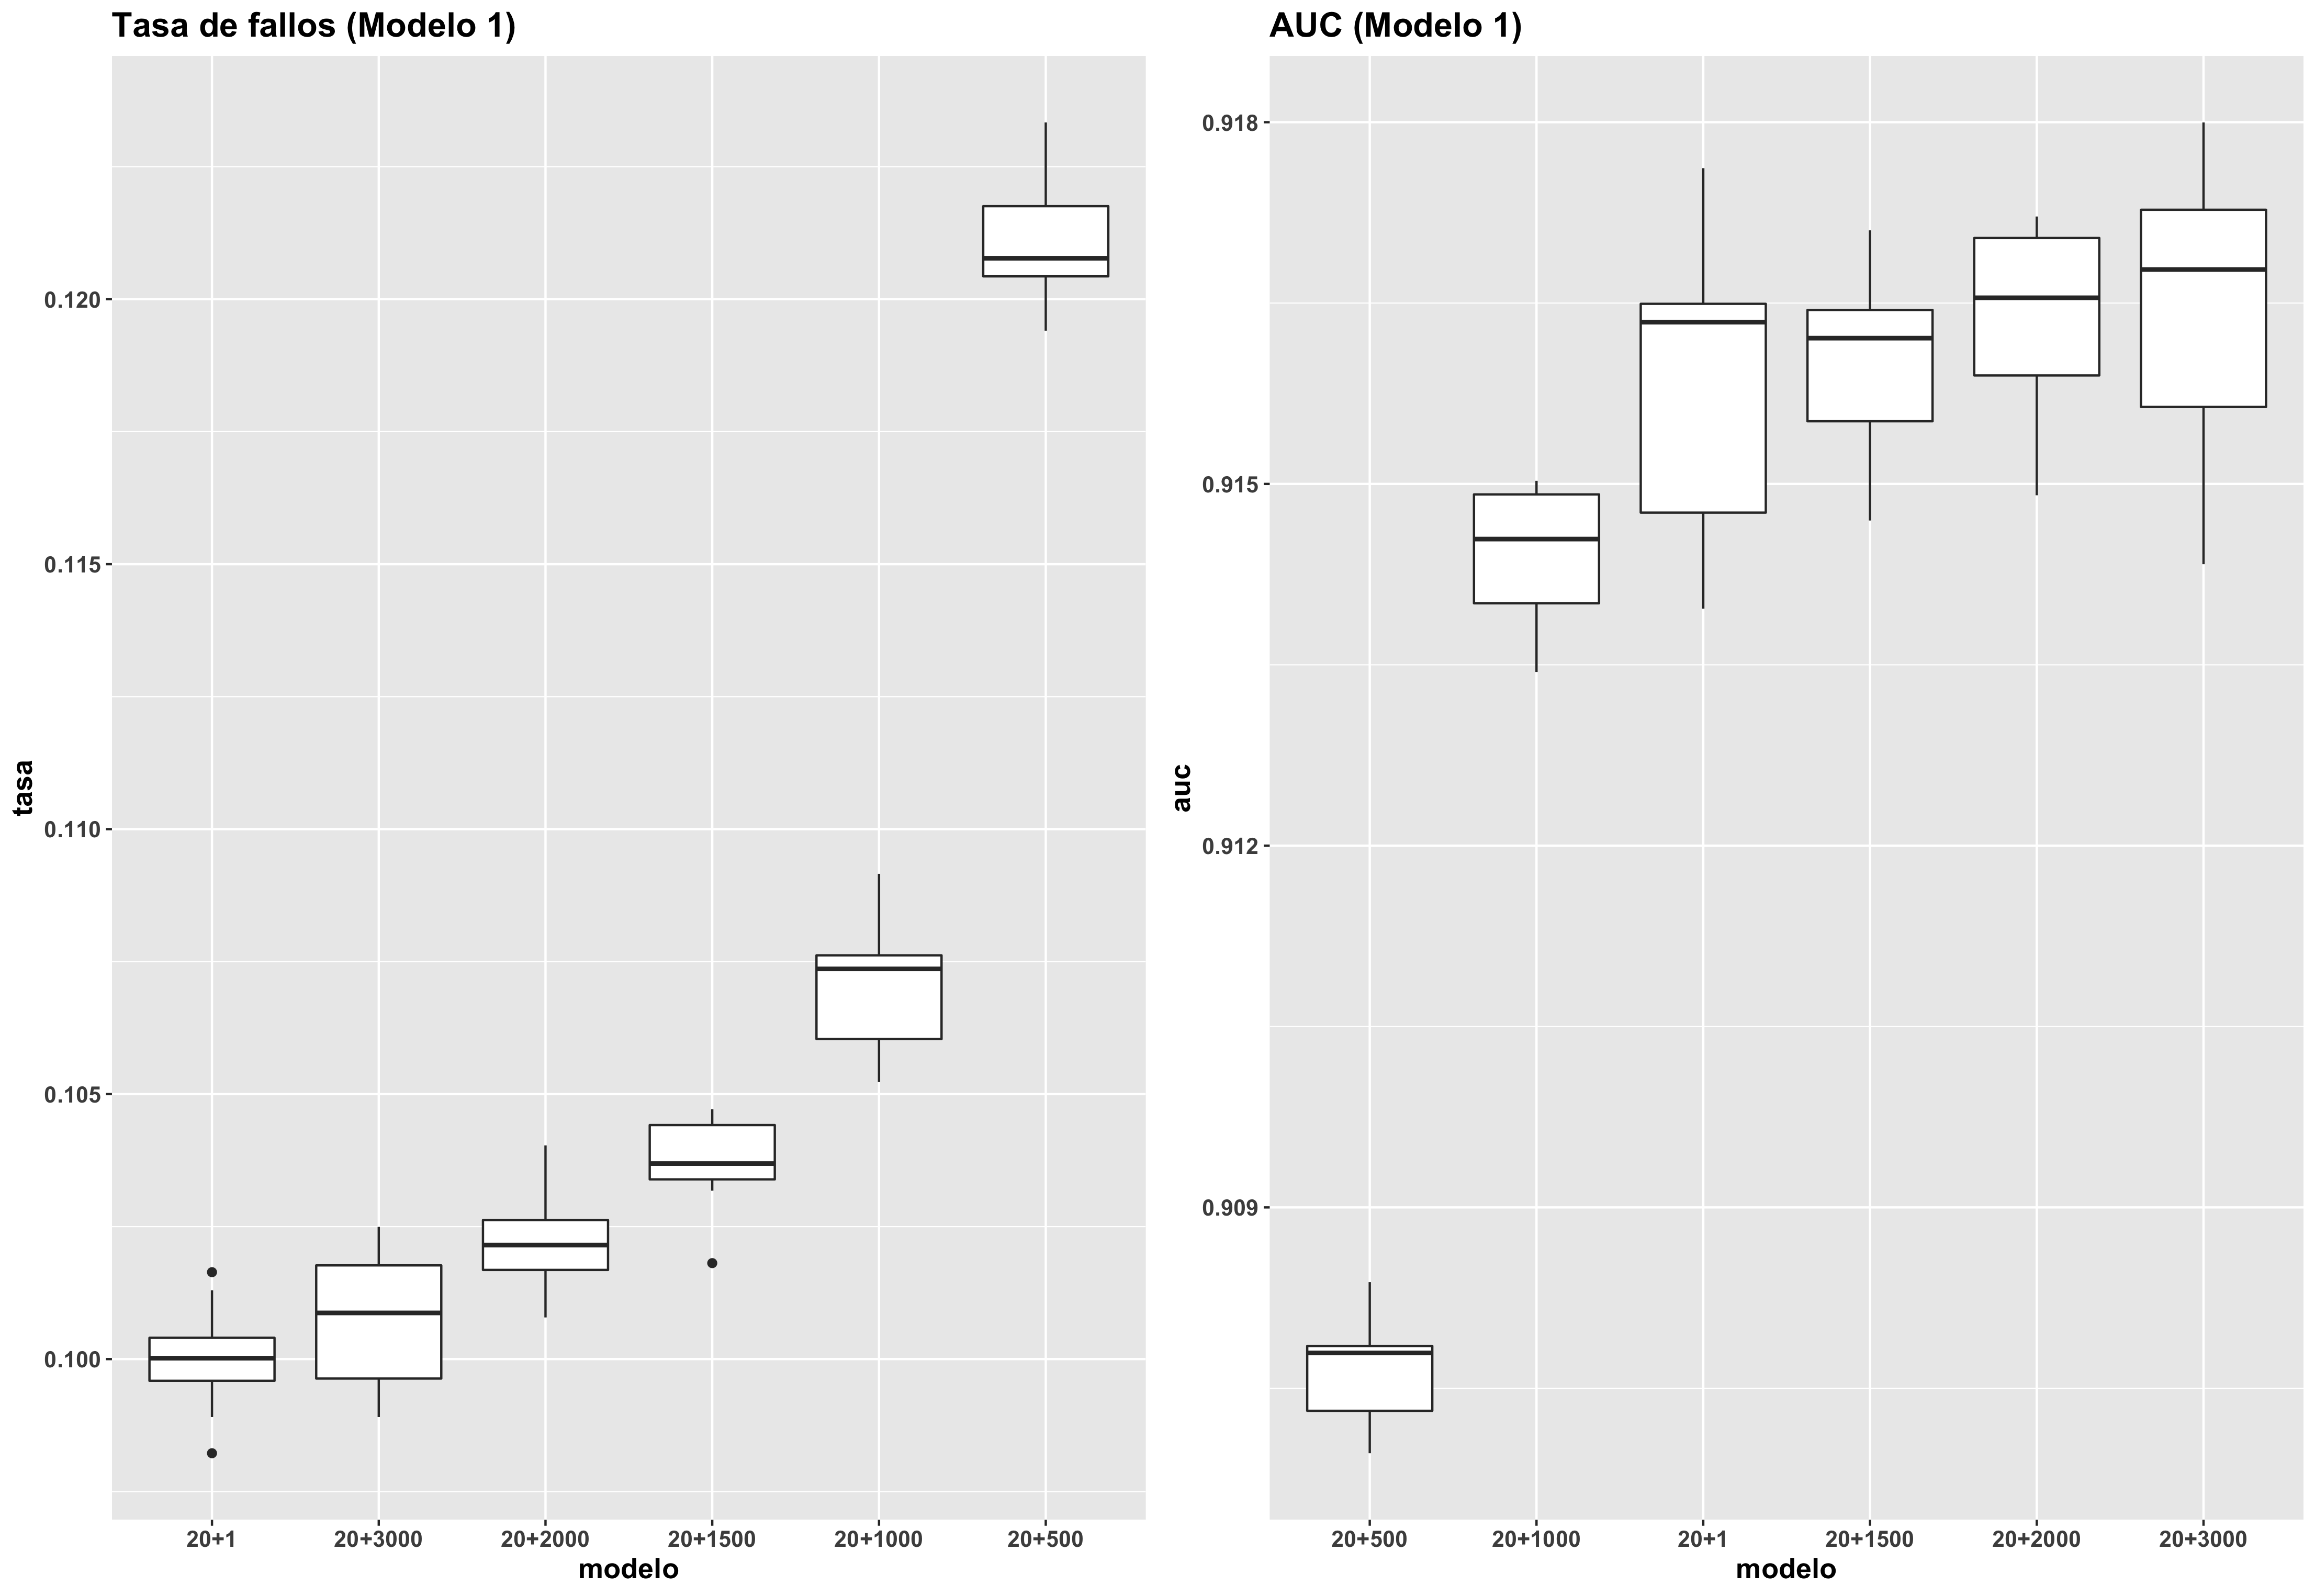
\includegraphics[width=0.99\linewidth,height=0.99\textheight,]{./charts/random_forest/04_comp_tasa_auc_modelo1_sampsizes} 

}

\caption{Tasa de fallos y AUC en funcion de  sampsize - Modelo 1}\label{fig:unnamed-chunk-93}
\end{figure}

Incluso sorteando variables, los resultados obtenido \textbf{no difieren
demasiado de un modelo \emph{bagging}}: mientras que con 500
observaciones la tasa de fallos aumenta hasta 0.12 y el AUC se reduce a
0.90, a partir de un tamaño de 1000 muestras (lo que supone alrededor
del 17 \% del total), \textbf{no solo iguala en AUC al resto de modelos
con \emph{sampsizes} mayores (en torno a 0.91), sino que además la
ganancia de error es de tan solo unas milésimas}: entre un
\emph{sampsize} = 1000 y 2000-3000 observaciones, la diferencia es de
0.107 - 0.102 = 0.005. Por tanto, \textbf{aumentar demasiado el tamaño
de las submuestras no aporta una mejoría significativa al modelo}, por
lo que nos decantamos por un valor de 1000.

Por último, para observar en mejor medida el efecto del parámetro
\emph{sampsize}, aumentamos a 10 grupos y 20 repeticiones:

\begin{figure}[h!]

{\centering 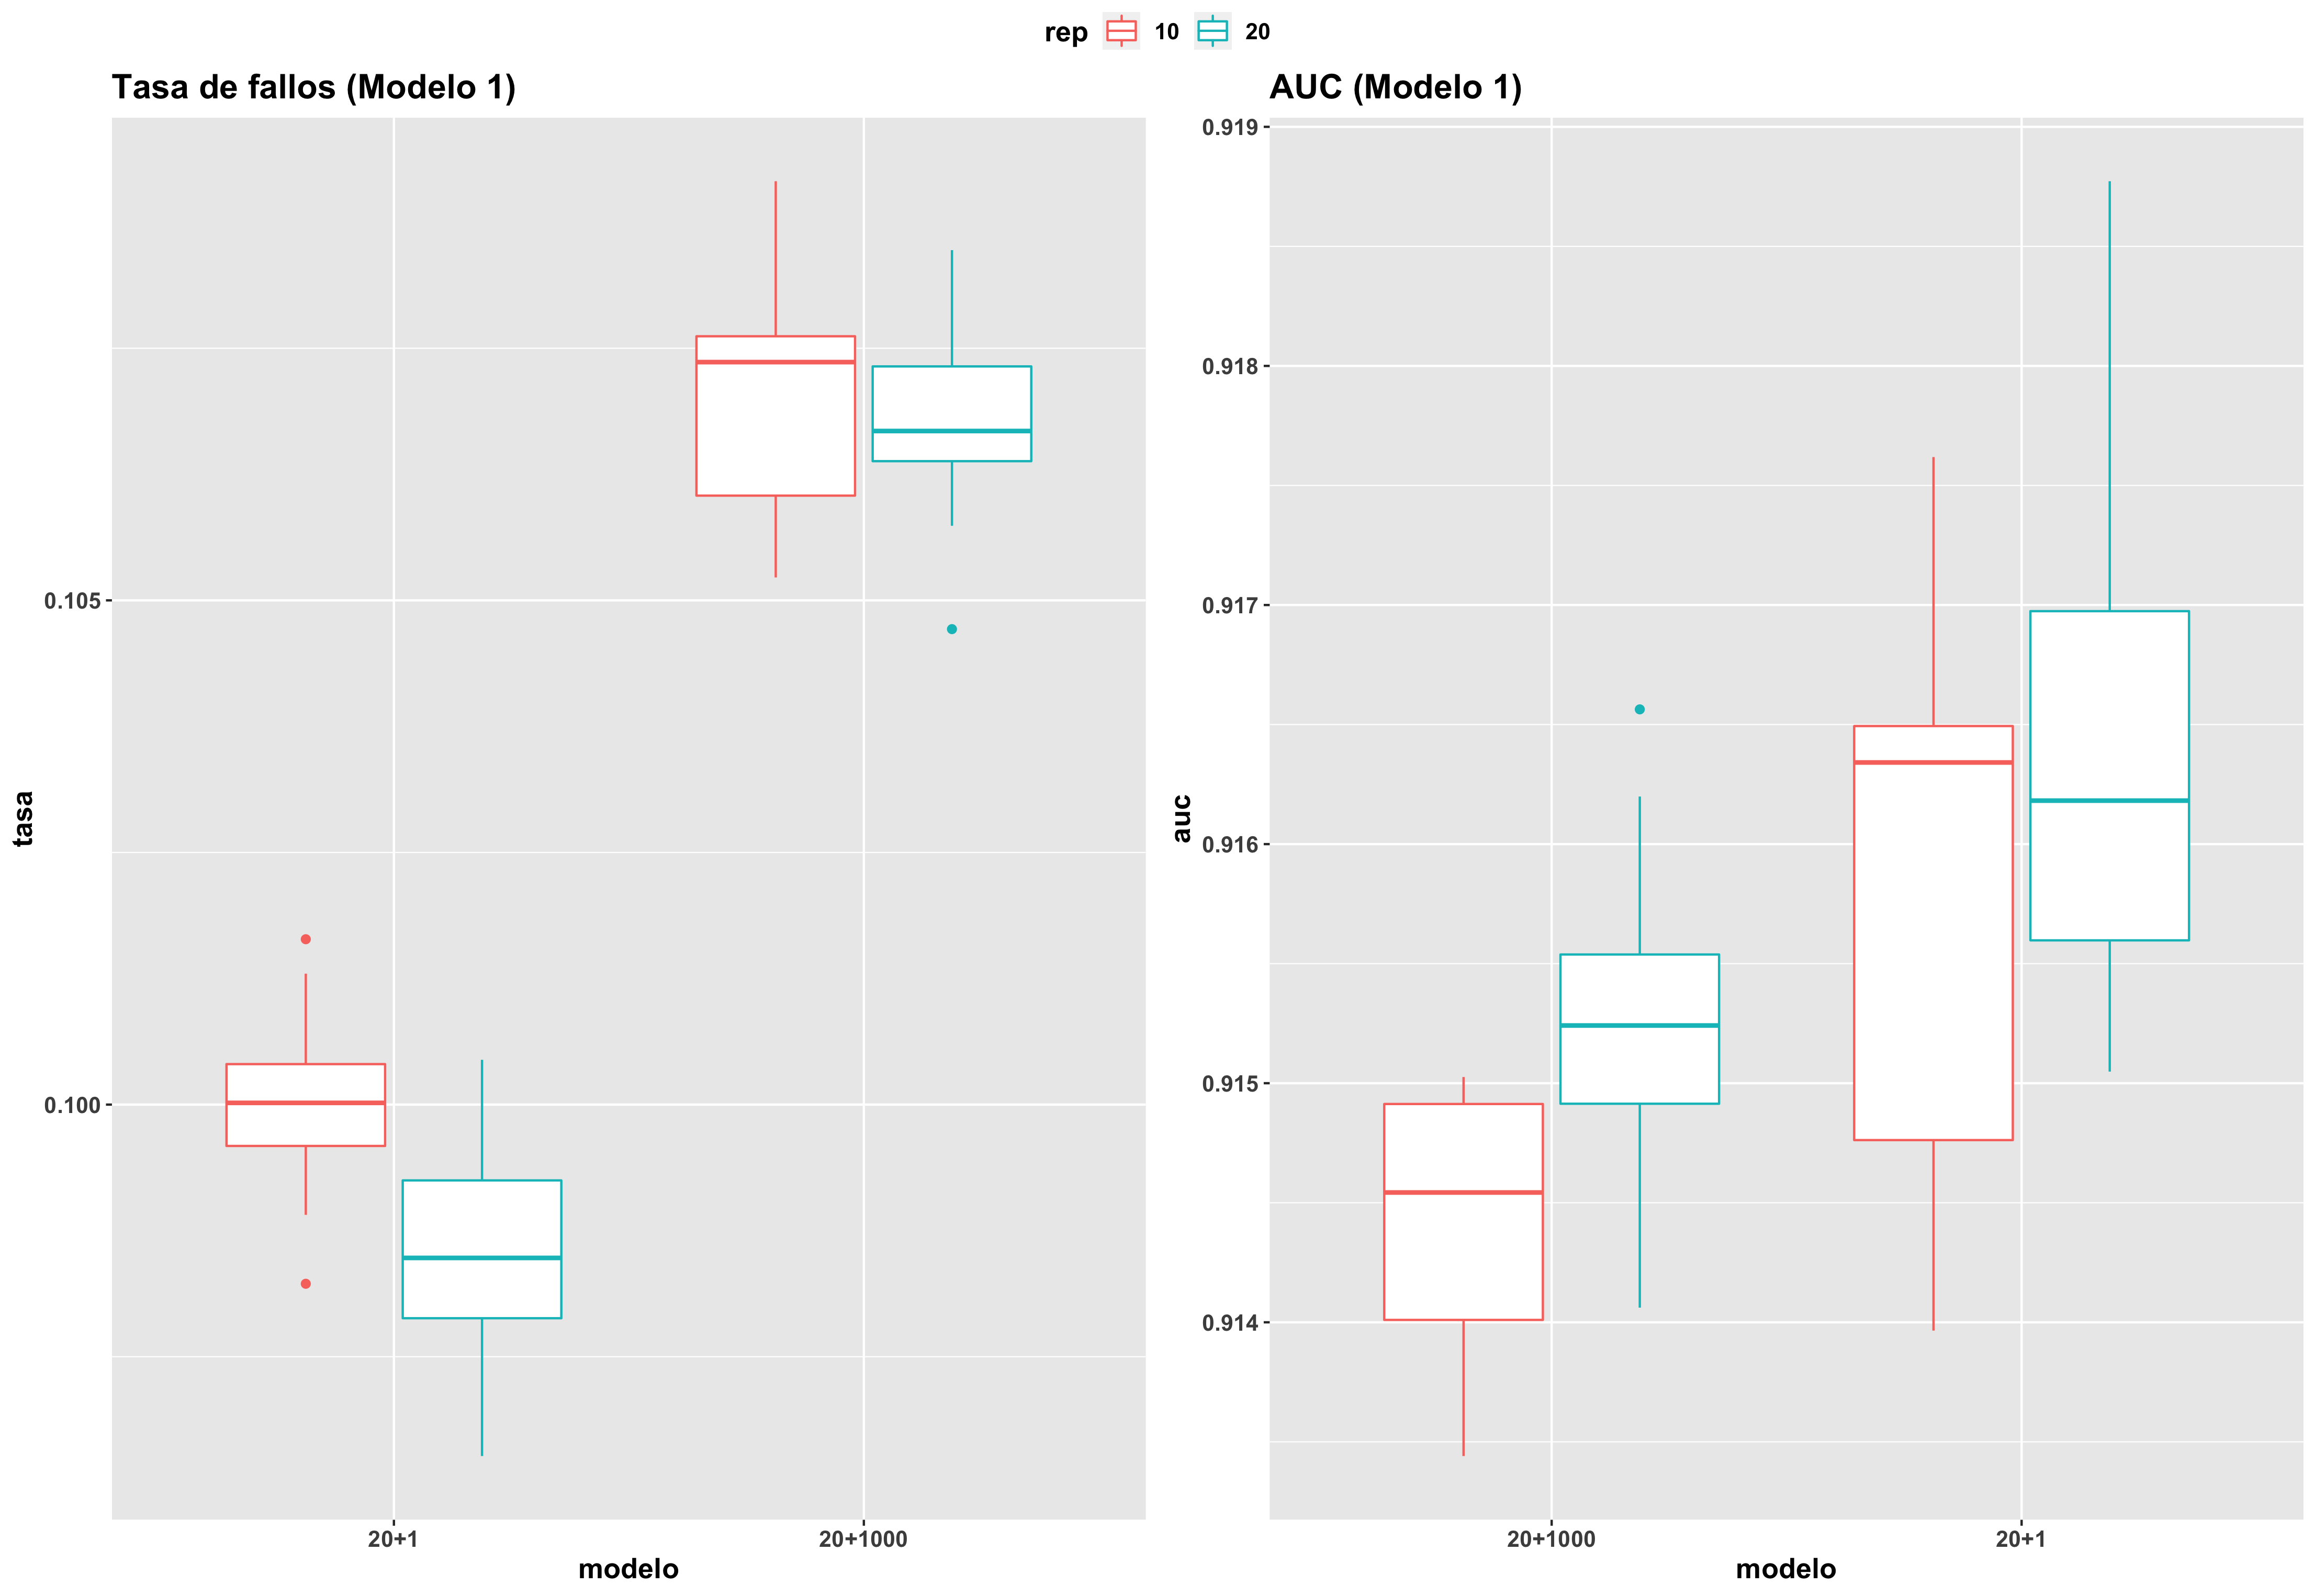
\includegraphics[width=0.99\linewidth,height=0.99\textheight,]{./charts/random_forest/04_comp_tasa_auc_modelo1_10_folds} 

}

\caption{Tasa de fallos y AUC aumentando a 10 grupos y 20 repeticiones - Modelo 1}\label{fig:unnamed-chunk-94}
\end{figure}

Incluso aumentando a 10 grupos y 20 repeticiones, tanto el sesgo como la
varianza se mantienen prácticamente idénticos.

\hypertarget{modelo-2-2}{%
\subsection{8.2 Modelo 2}\label{modelo-2-2}}

A continuación, realizamos los mismos pasos con el segundo \emph{set} de
variables, parametrizando en primer lugar tanto \emph{nodesize} como
\emph{sampsize}:

\begin{Shaded}
\begin{Highlighting}[]
\NormalTok{sampsizes}\FloatTok{.2}\NormalTok{ <{-}}\StringTok{ }\KeywordTok{list}\NormalTok{(}\DecValTok{1}\NormalTok{, }\DecValTok{100}\NormalTok{, }\DecValTok{500}\NormalTok{, }\DecValTok{1000}\NormalTok{, }\DecValTok{2000}\NormalTok{, }\DecValTok{3000}\NormalTok{, }\DecValTok{4600}\NormalTok{)}
\NormalTok{nodesizes}\FloatTok{.2}\NormalTok{ <{-}}\StringTok{ }\KeywordTok{list}\NormalTok{(}\DecValTok{5}\NormalTok{, }\DecValTok{10}\NormalTok{, }\DecValTok{20}\NormalTok{, }\DecValTok{30}\NormalTok{, }\DecValTok{40}\NormalTok{, }\DecValTok{50}\NormalTok{, }\DecValTok{100}\NormalTok{)}

\CommentTok{\# Tuneamos nuevamente tanto sampsizes como nodesizes}
\NormalTok{bagging\_modelo2\_mtry2 <{-}}\StringTok{  }\KeywordTok{tuneo\_rf}\NormalTok{(surgical\_dataset, }\DataTypeTok{target =}\NormalTok{ target,}
                                   \DataTypeTok{lista.continua =}\NormalTok{ var\_modelo2,}
                                   \DataTypeTok{nodesizes =}\NormalTok{ nodesizes}\FloatTok{.2}\NormalTok{,}
                                   \DataTypeTok{sampsizes =}\NormalTok{ sampsizes}\FloatTok{.2}\NormalTok{, }\DataTypeTok{mtry =} \DecValTok{2}\NormalTok{,}
                                   \DataTypeTok{ntree =} \DecValTok{2000}\NormalTok{, }\DataTypeTok{grupos =} \DecValTok{5}\NormalTok{, }\DataTypeTok{repe =} \DecValTok{5}\NormalTok{)}
\end{Highlighting}
\end{Shaded}

\begin{figure}[h!]

{\centering 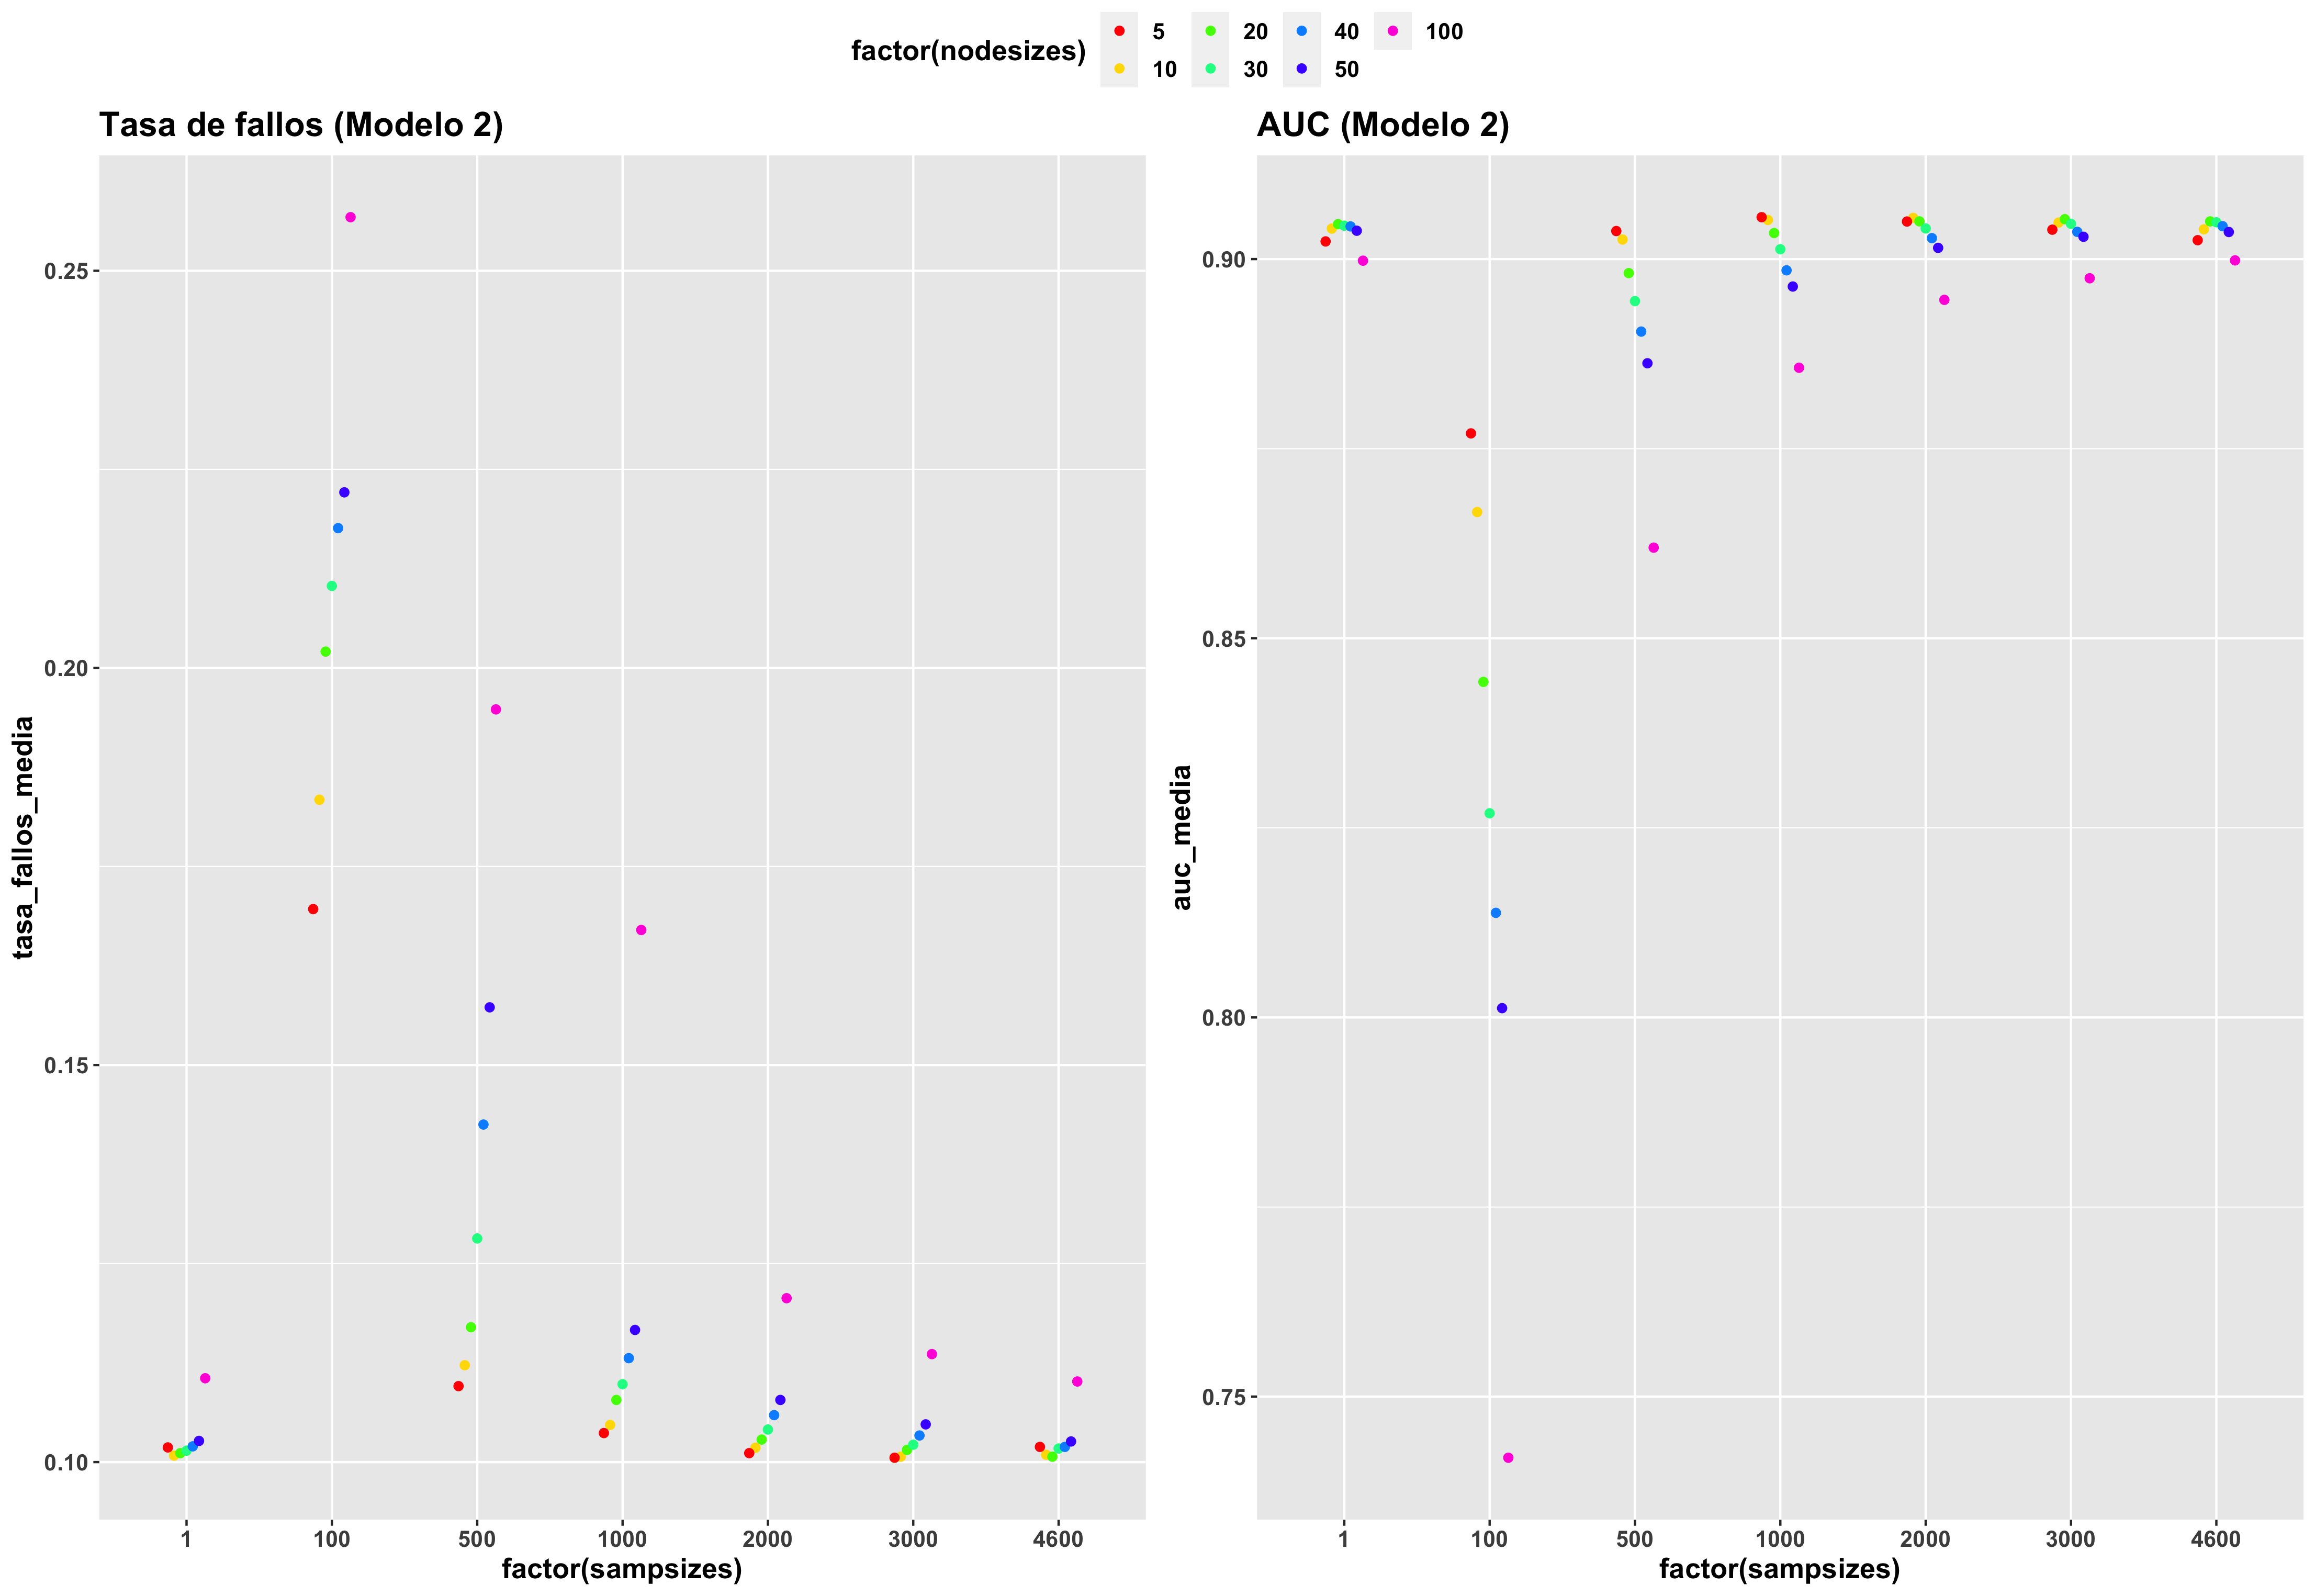
\includegraphics[width=0.99\linewidth,height=0.99\textheight,]{./charts/random_forest/04_comp_tasa_auc_modelo2} 

}

\caption{Tasa de fallos y AUC en funcion de nodesize y sampsize - Modelo 2}\label{fig:unnamed-chunk-96}
\end{figure}

Del mismo modo que sucede con el primer \emph{set} de variables, tanto
con un \emph{nodesize} en torno a 20 como un valor \emph{sampsize} entre
500 y 1000, parece una buena opción. Además, si analizamos tanto el
sesgo como la varianza al variar este último parámetro, aumentando a 10
el número de repeticiones:

\begin{figure}[h!]

{\centering 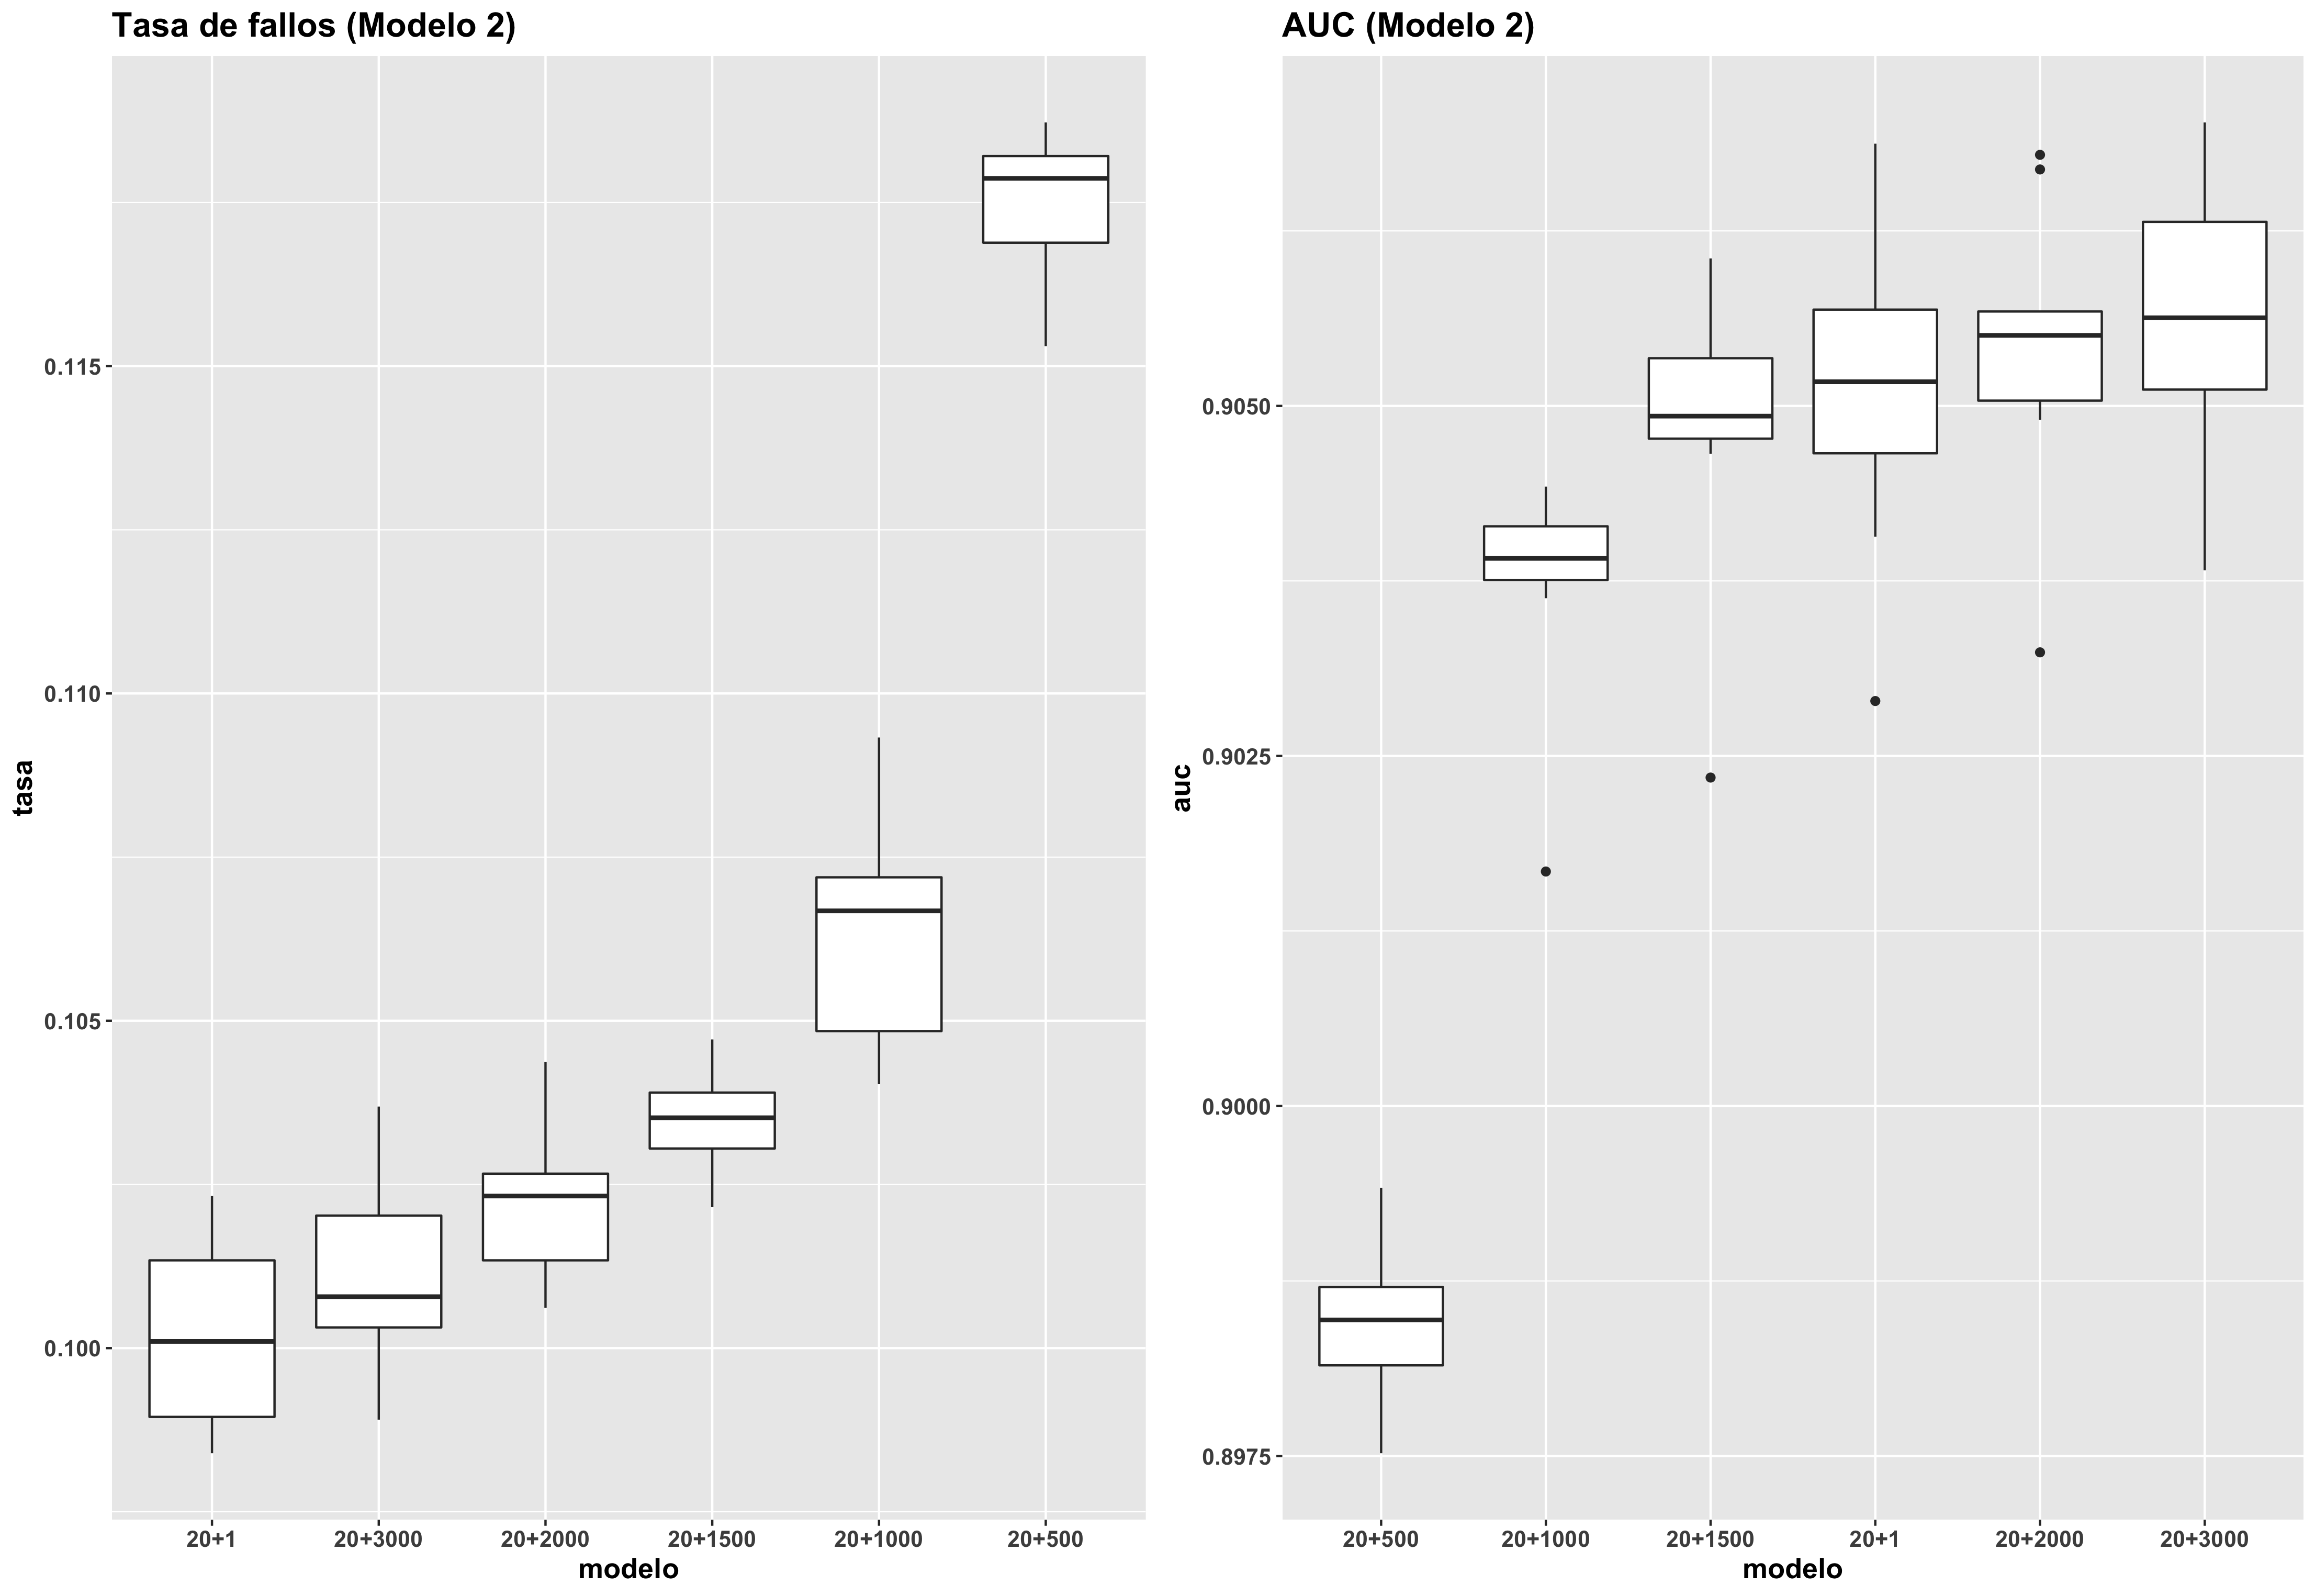
\includegraphics[width=0.99\linewidth,height=0.99\textheight,]{./charts/random_forest/04_comp_tasa_auc_modelo2_sampsizes} 

}

\caption{Tasa de fallos y AUC en funcion de  sampsize - Modelo 2}\label{fig:unnamed-chunk-97}
\end{figure}

Tenemos el mismo comportamiento que el primer \emph{set} de variables:
\textbf{a partir de un tamaño en torno a 1000 observaciones, la
diferencia tanto en la tasa de fallos como en \emph{AUC} es muy
pequeña}, por lo que no merece la pena aumentar aun más el tamaño de la
muestra. Incluso si aumentamos el número de grupos y repeticiones a 10 y
20, respectivamente:

\begin{figure}[h!]

{\centering 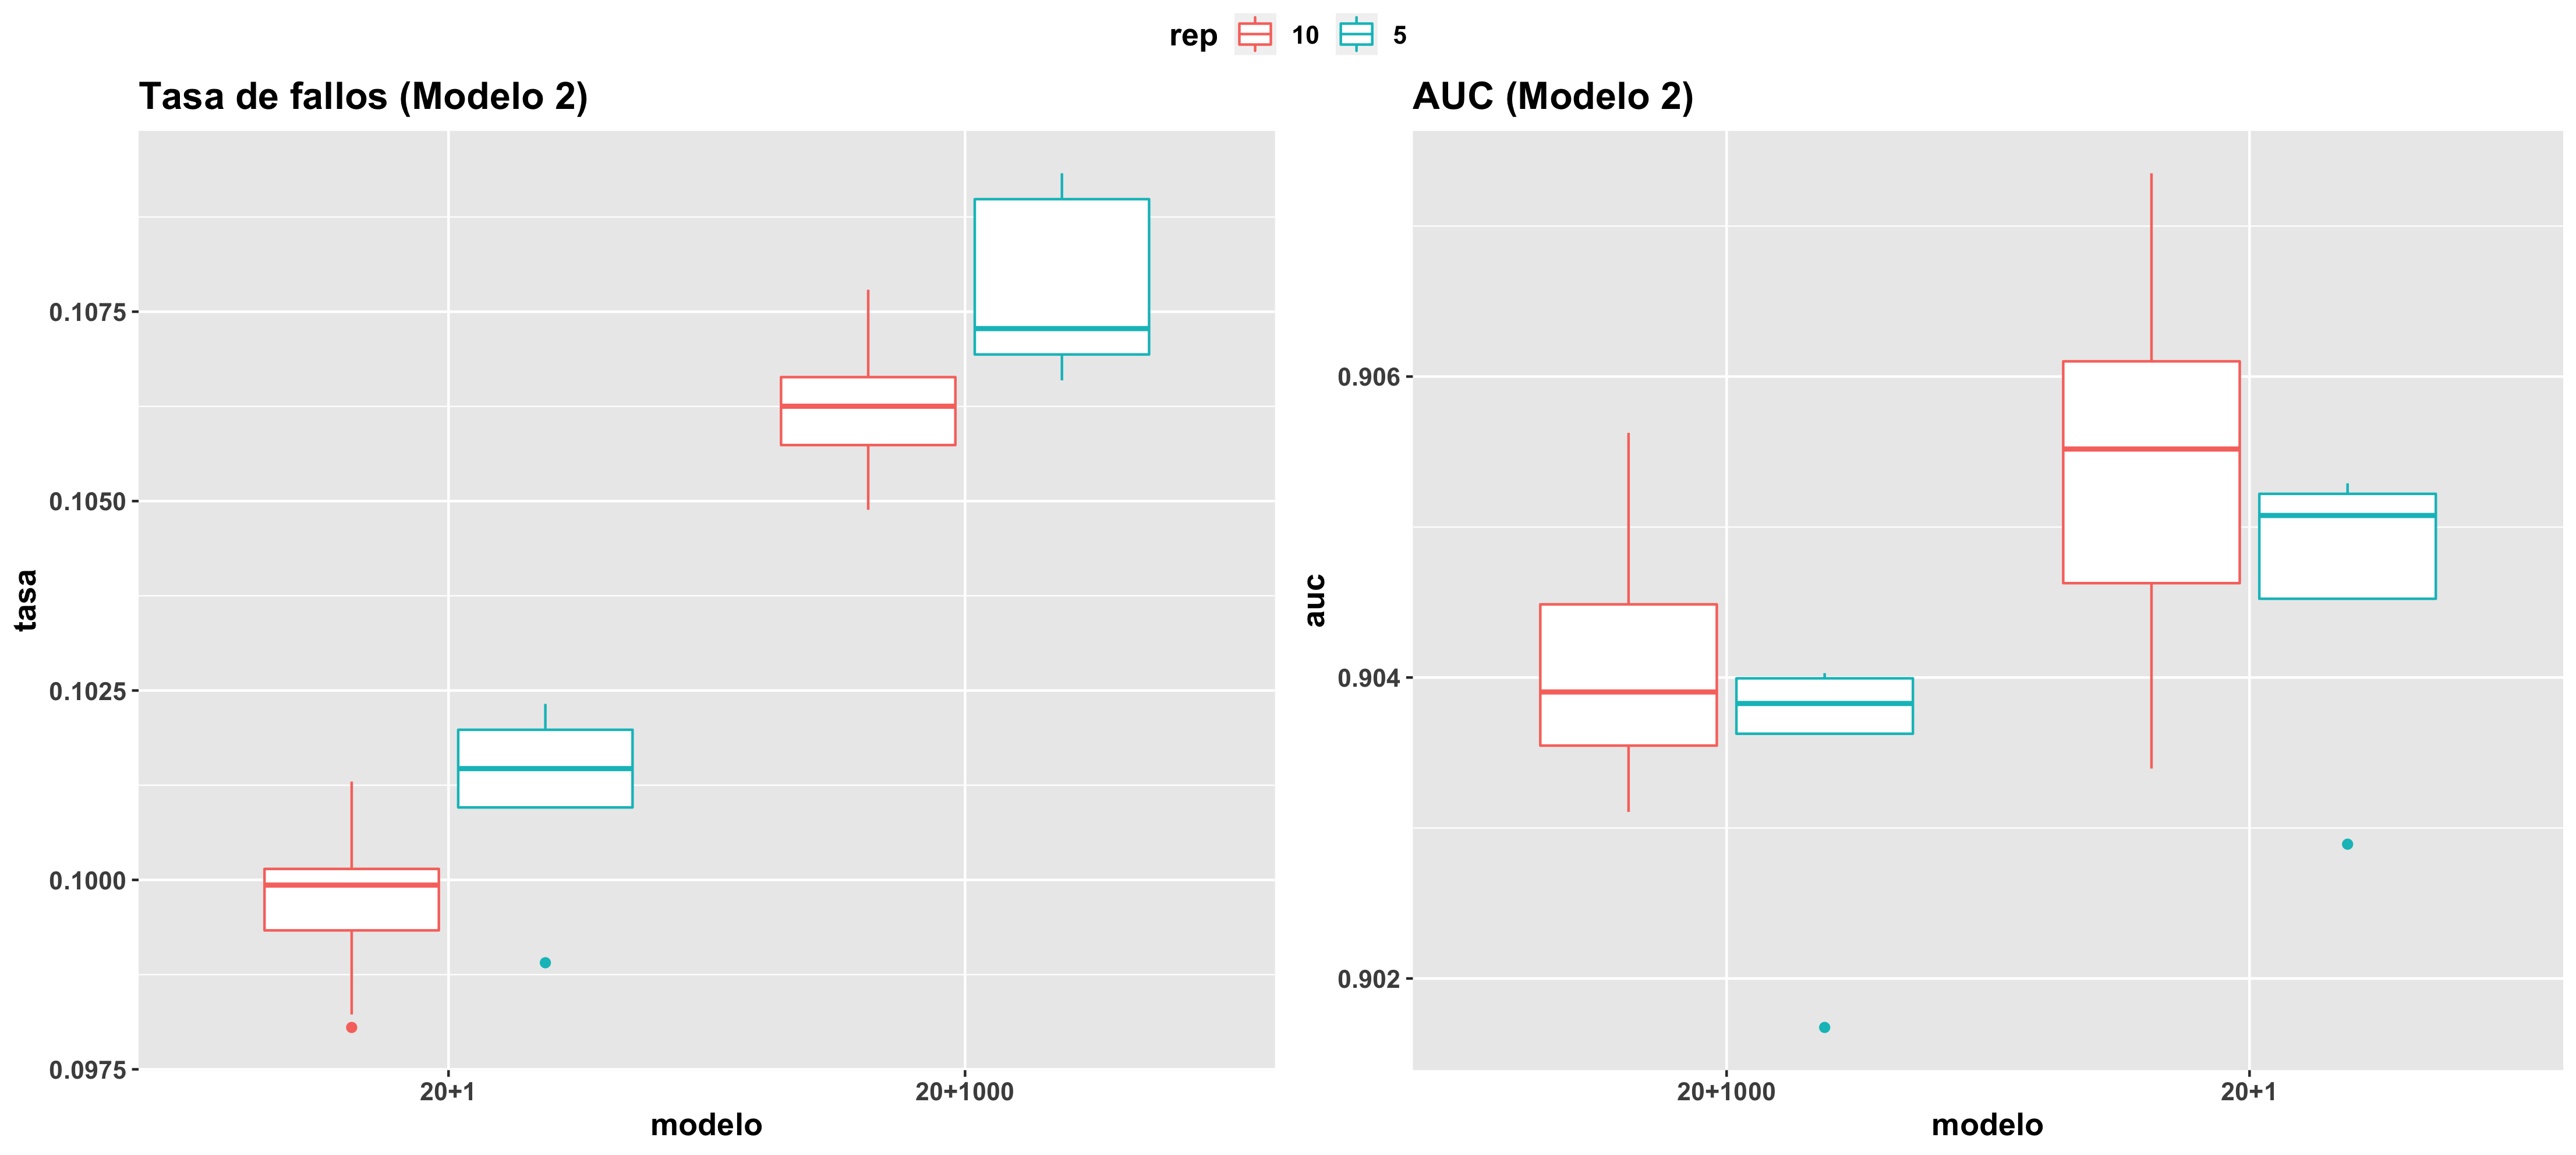
\includegraphics[width=0.99\linewidth,height=0.99\textheight,]{./charts/random_forest/04_comp_tasa_auc_modelo2_sampsizes2_10_folds} 

}

\caption{Tasa de fallos y AUC aumentando a 10 grupos y 20 repeticiones - Modelo 2}\label{fig:unnamed-chunk-98}
\end{figure}

El orden de los modelos se mantiene idéntico. Por tanto, dado que el
valor AUC es prácticamente el mismo, además de que la ganancia de la
tasa de fallos es muy pequeña (dada la escala del eje), nos decantamos
nuevamente por un modelo con \emph{sampsize} = 1000.

\textbf{RESUMEN \emph{random forest}}:

\begin{enumerate}
\def\labelenumi{\arabic{enumi}.}
\tightlist
\item
  modelo 1: \emph{mtry} = 3, \emph{nodesize} = 20 y \emph{sampsize} =
  1000.
\item
  modelo 2: \emph{mtry} = 2, \emph{nodesize} = 20 y \emph{sampsize} =
  1000.
\end{enumerate}

\hypertarget{modelo-sin-reemplazamiento-1}{%
\subsection{8.3 Modelo sin
reemplazamiento}\label{modelo-sin-reemplazamiento-1}}

Una vez tuneados ambos \emph{sets} de variables, veamos la diferencia
entre un modelo con \emph{sampsize} con reemplazamiento y sin
reemplazamiento:

\begin{Shaded}
\begin{Highlighting}[]
\CommentTok{\#{-}{-} ¿Y si lo probamos sin reemplazamiento? Probamos con el mejor modelo en terminos de AUC (modelo 1)}
\NormalTok{bagging\_modelo\_sin\_reemp <{-}}\StringTok{ }\KeywordTok{tuneo\_rf}\NormalTok{(surgical\_dataset, }\DataTypeTok{target =}\NormalTok{ target,}
                                     \DataTypeTok{lista.continua =}\NormalTok{ var\_modelo1, }\DataTypeTok{nodesizes =} \DecValTok{20}\NormalTok{, }
                                     \DataTypeTok{sampsizes =} \DecValTok{1000}\NormalTok{, }\DataTypeTok{mtry =} \DecValTok{3}\NormalTok{, }\DataTypeTok{ntree =} \DecValTok{2000}\NormalTok{, }
                                     \DataTypeTok{grupos =} \DecValTok{5}\NormalTok{, }\DataTypeTok{repe =} \DecValTok{10}\NormalTok{, }\DataTypeTok{replace =} \OtherTok{FALSE}\NormalTok{)}
\end{Highlighting}
\end{Shaded}

\begin{figure}[h!]

{\centering 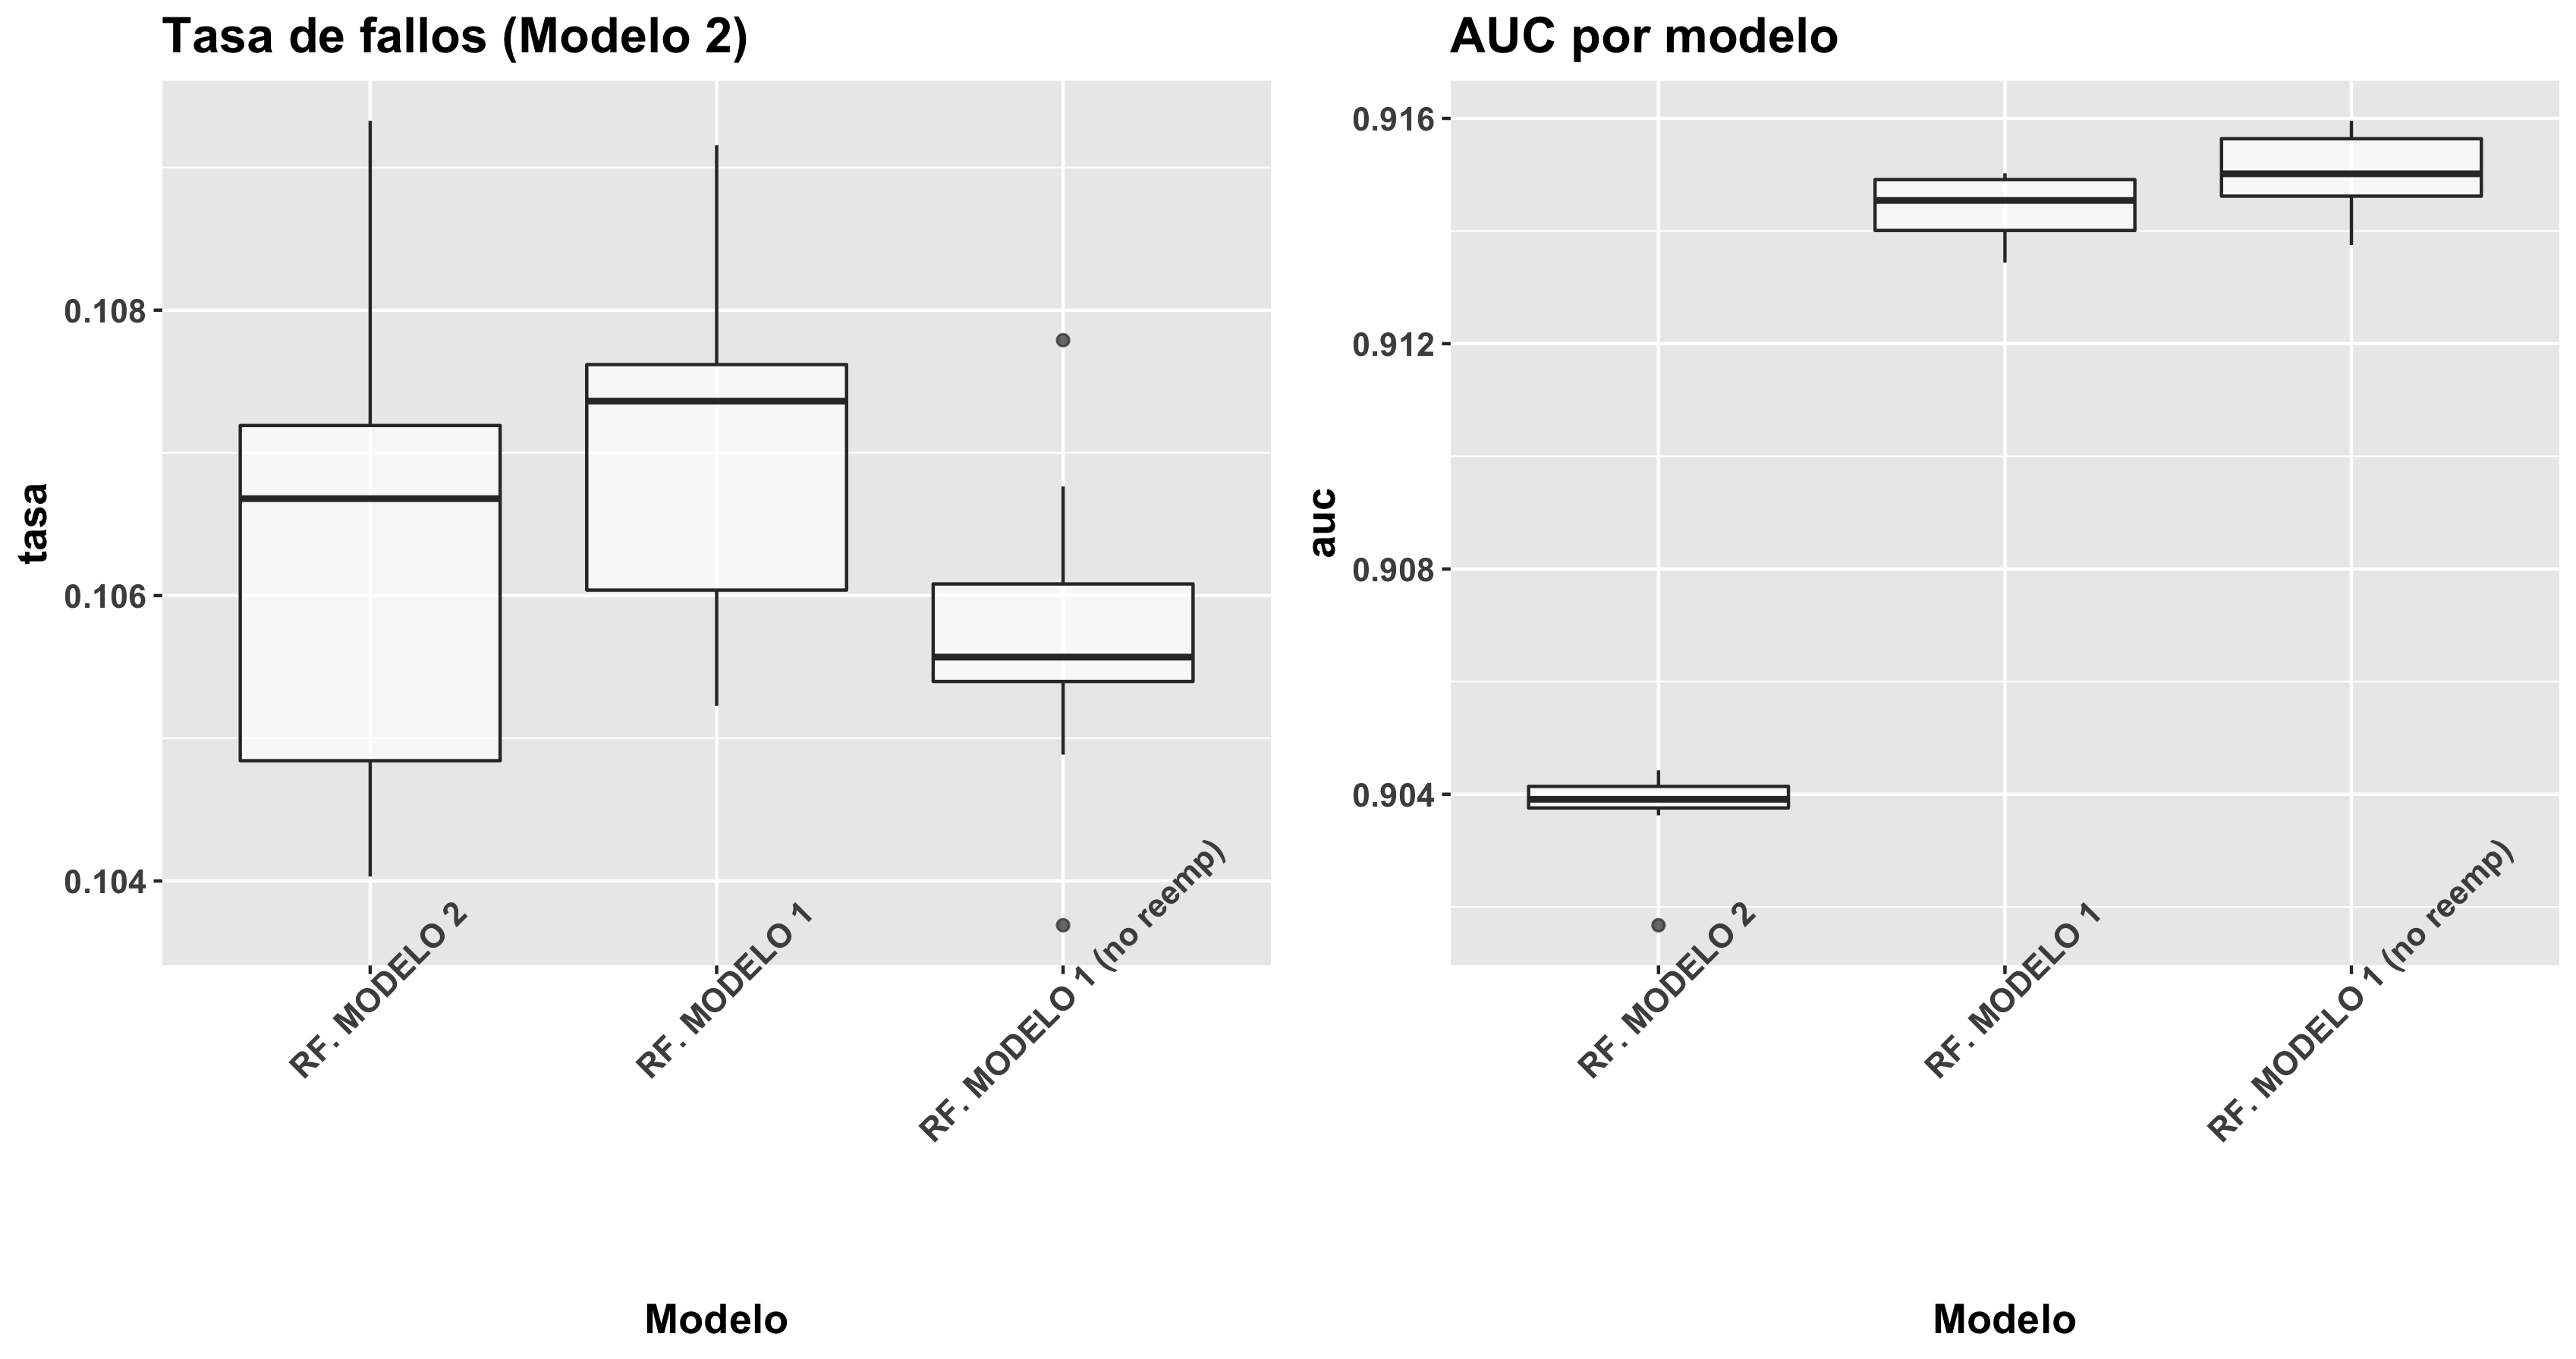
\includegraphics[width=0.99\linewidth,height=0.99\textheight,]{./charts/comparativas/03_rf_con_sin_reemp} 

}

\caption{Comparación Random Forest con o sin reemplazamiento}\label{fig:unnamed-chunk-100}
\end{figure}

Como podemos comprobar, el hecho de seleccionar muestras con o sin
reemplazamiento \textbf{no aporta mejoría alguna al modelo}.

\hypertarget{comparaciuxf3n-final-2}{%
\subsection{8.4 Comparación final}\label{comparaciuxf3n-final-2}}

Por último, realizamos la comparación final de ambos modelos
\emph{random forest} con los datos \emph{test}:

\begin{verbatim}
##                 modelo precision sensibilidad especificidad valor_pred_pos
## 1 Modelo 1 (BIC TOP 5)    0.8990       0.9052        0.8976         0.6639
## 2     Modelo 2 (top 4)    0.8964       0.9117        0.8931         0.6465
##   valor_pred_neg
## 1         0.9769
## 2         0.9792
\end{verbatim}

En base a los resultados obtenidos, no se diferencia demasiado de un
modelo \emph{bagging}:

\begin{verbatim}
##                 modelo precision sensibilidad especificidad valor_pred_pos
## 1 Modelo 1 (BIC TOP 5)    0.9010       0.9214        0.8966         0.6589
## 2     Modelo 2 (top 4)    0.9019       0.9468        0.8928         0.6424
##   valor_pred_neg
## 1         0.9813
## 2         0.9880
\end{verbatim}

\begin{enumerate}
\def\labelenumi{\arabic{enumi}.}
\tightlist
\item
  \textbf{Precisión}: de 0.901 y 0.9019 a 0.899 y 0.8964 en ambos
  \emph{sets} de variables, respectivamente.
\item
  \textbf{Sensibilidad}: de 0.9214 y 0.9468 a 0.9052 y 0.9117,
  respectivamente (empeora ligeramente).
\item
  \textbf{Especificidad}: tanto en \emph{bagging} como en \emph{random
  forest} se sitúa en torno a 0.89.
\item
  \textbf{Valor predictivo positivo}: continúa situándose en torno a
  0.64-0.65-0.66.
\item
  \textbf{Valor predictivo negativo}: continúa situándose en torno a
  0.97-0.98.
\end{enumerate}

Es decir, \textbf{añadiendo el sorteo de variables al modelo (mtry), la
variación que experimenta en el conjunto \emph{test} es muy pequeña}. De
hecho, si observamos la distribución de la tasa de fallos y AUC:

\begin{figure}[h!]

{\centering 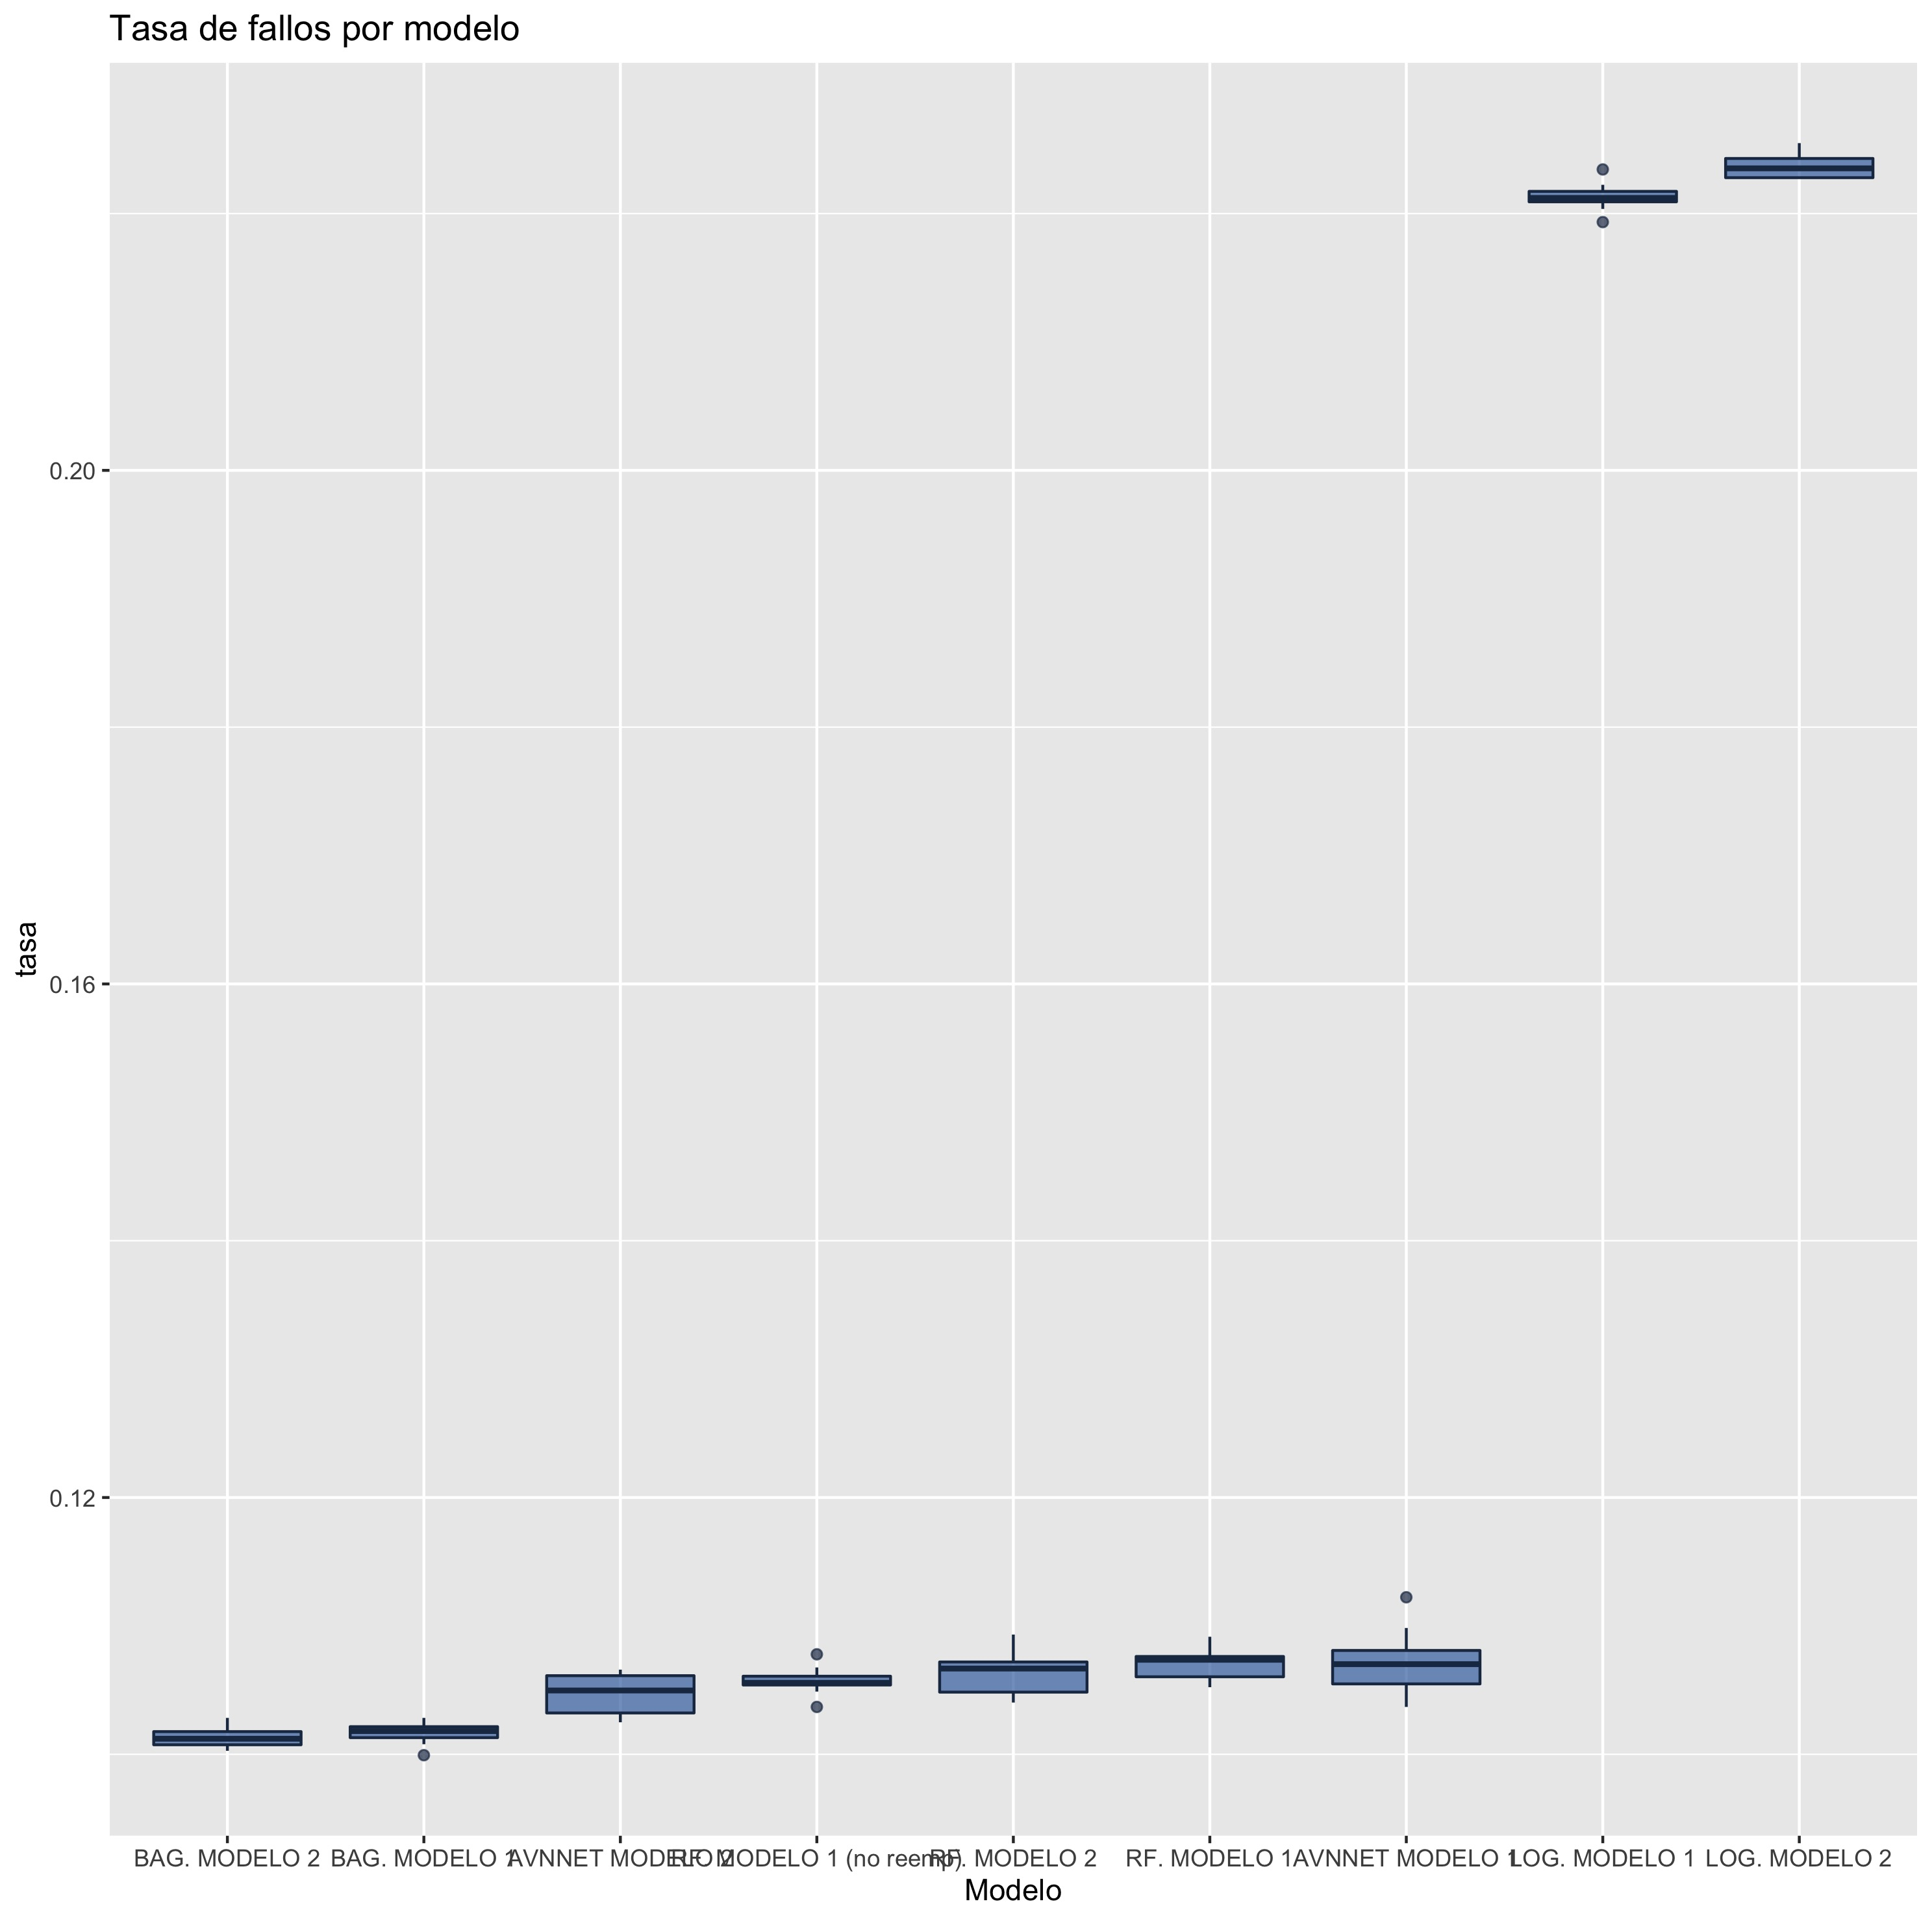
\includegraphics[width=0.99\linewidth,height=0.99\textheight,]{./charts/comparativas/03_log_avnnet_bagging_rf_tasa} 

}

\caption{Comparacion tasa fallos log-avnnet-bagging-rf}\label{fig:unnamed-chunk-103}
\end{figure}
\begin{figure}[h!]

{\centering 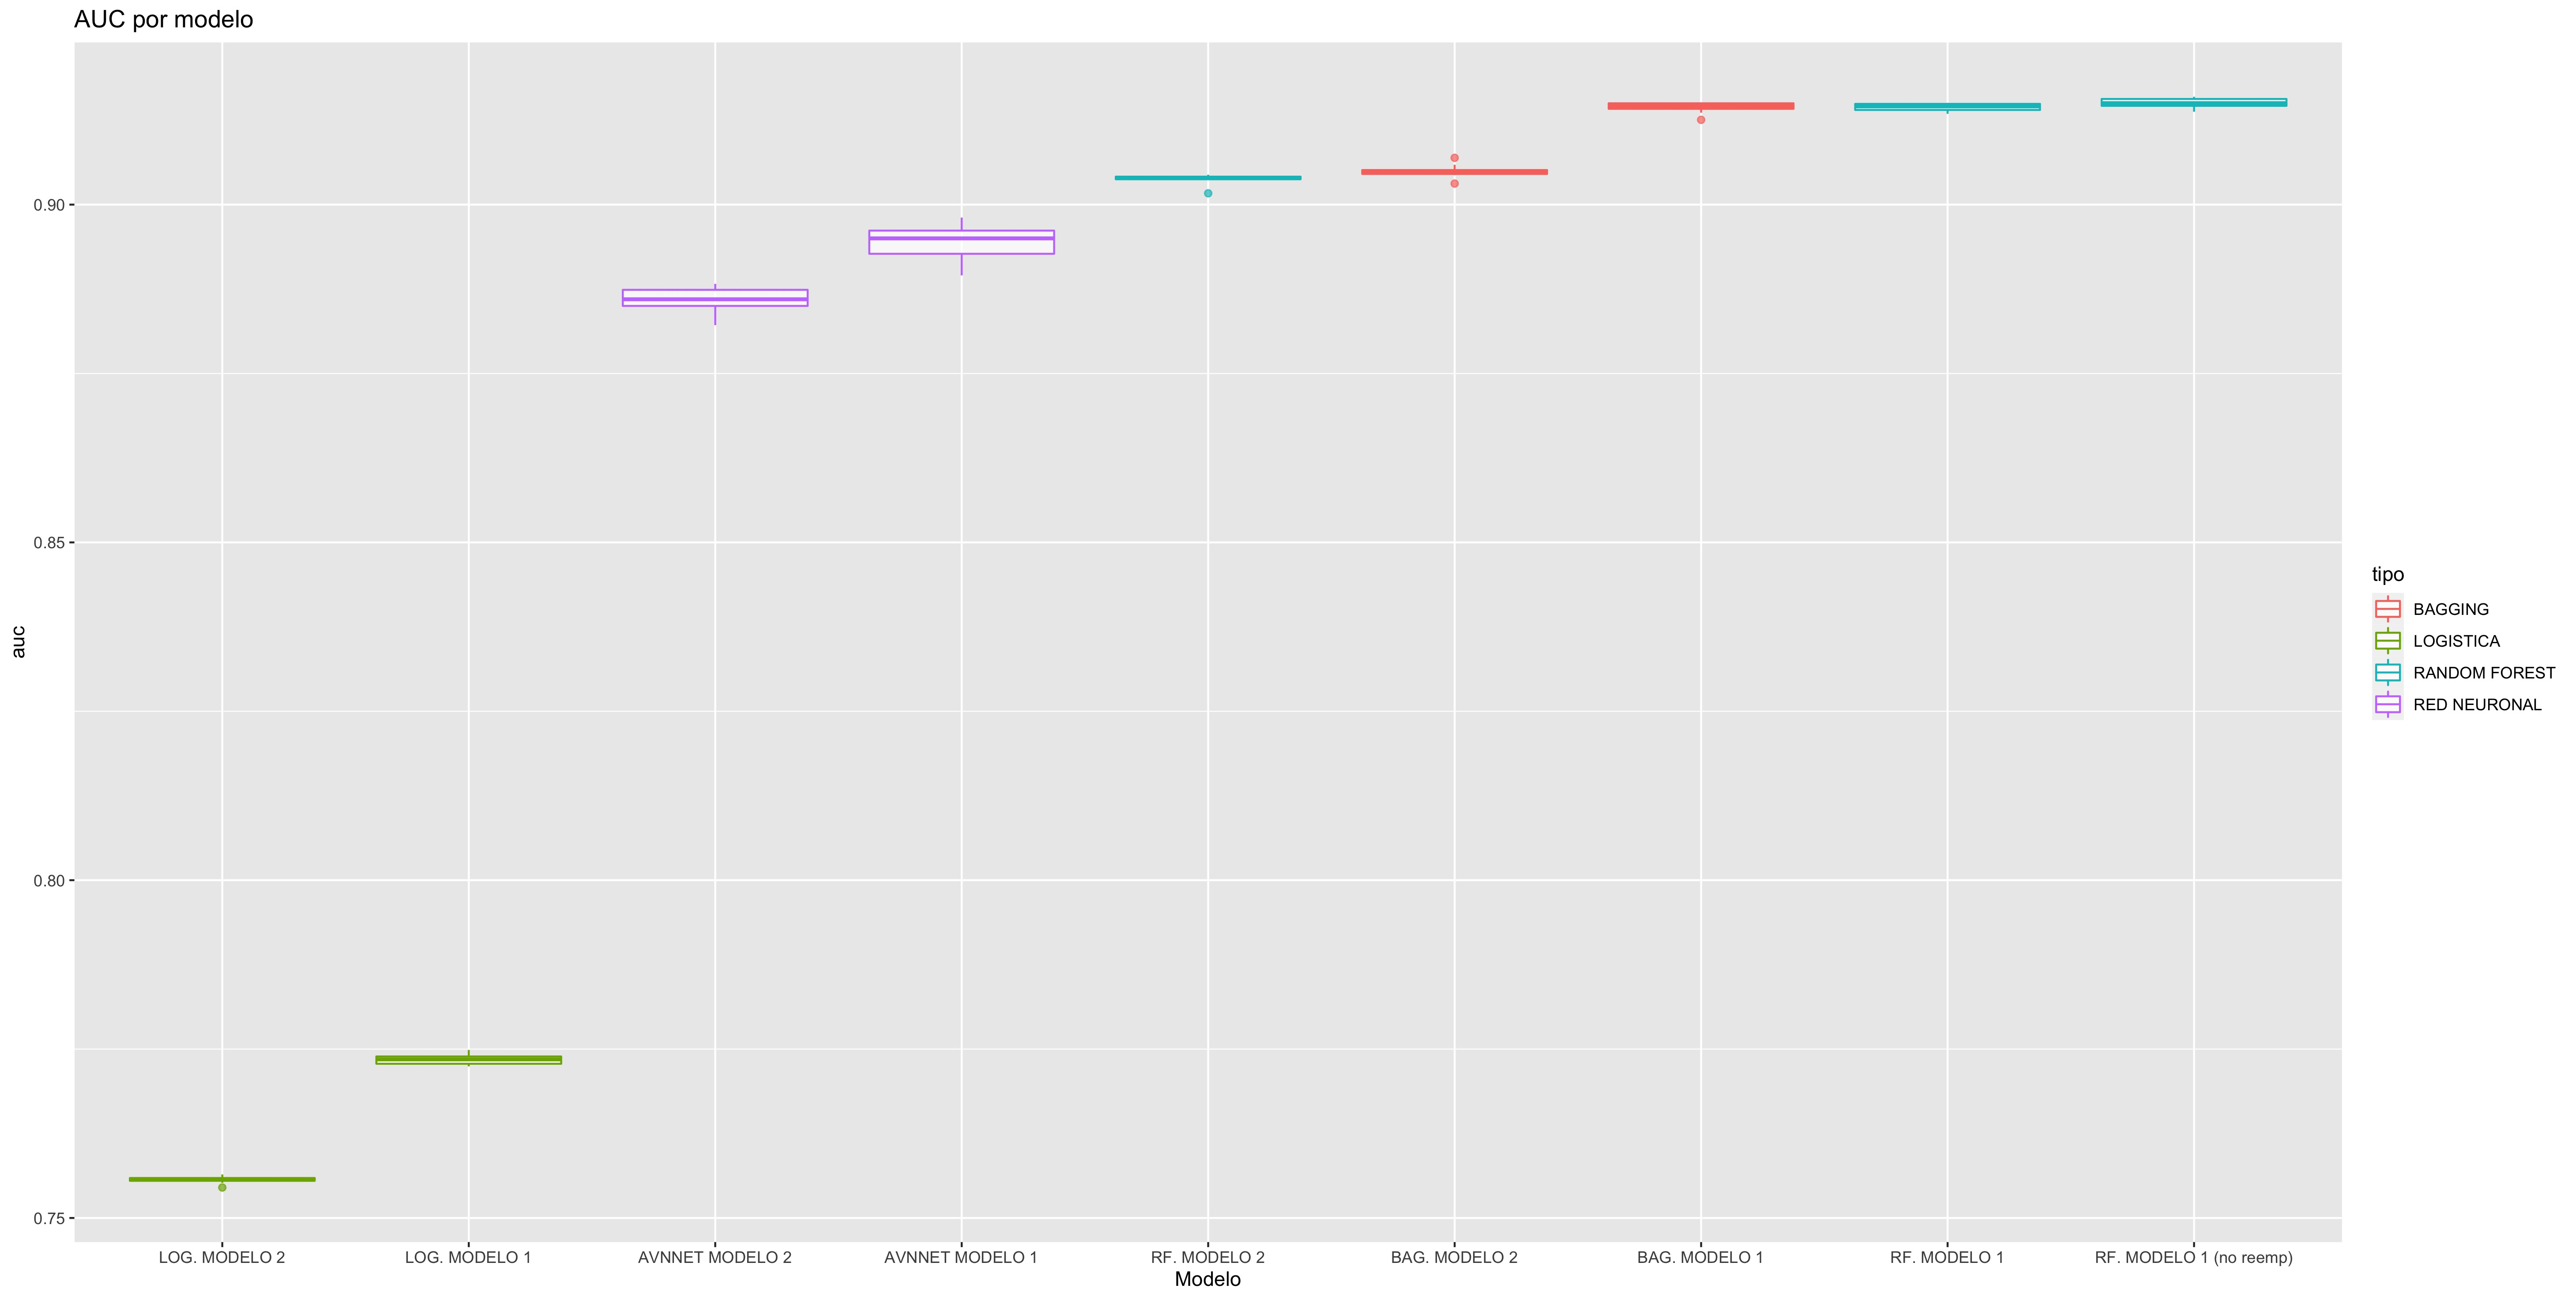
\includegraphics[width=0.99\linewidth,height=0.99\textheight,]{./charts/comparativas/03_log_avnnet_bagging_rf_auc} 

}

\caption{Comparacion AUC log-avnnet-bagging-rf}\label{fig:unnamed-chunk-104}
\end{figure}

En relación al resto de modelos, \emph{random forest} se situa a la
misma altura que modelos como \emph{bagging} o \emph{avnnet}. De hecho,
si hacemos ``zoom'' sobre los modelos de árbol:

\begin{figure}[h!]

{\centering 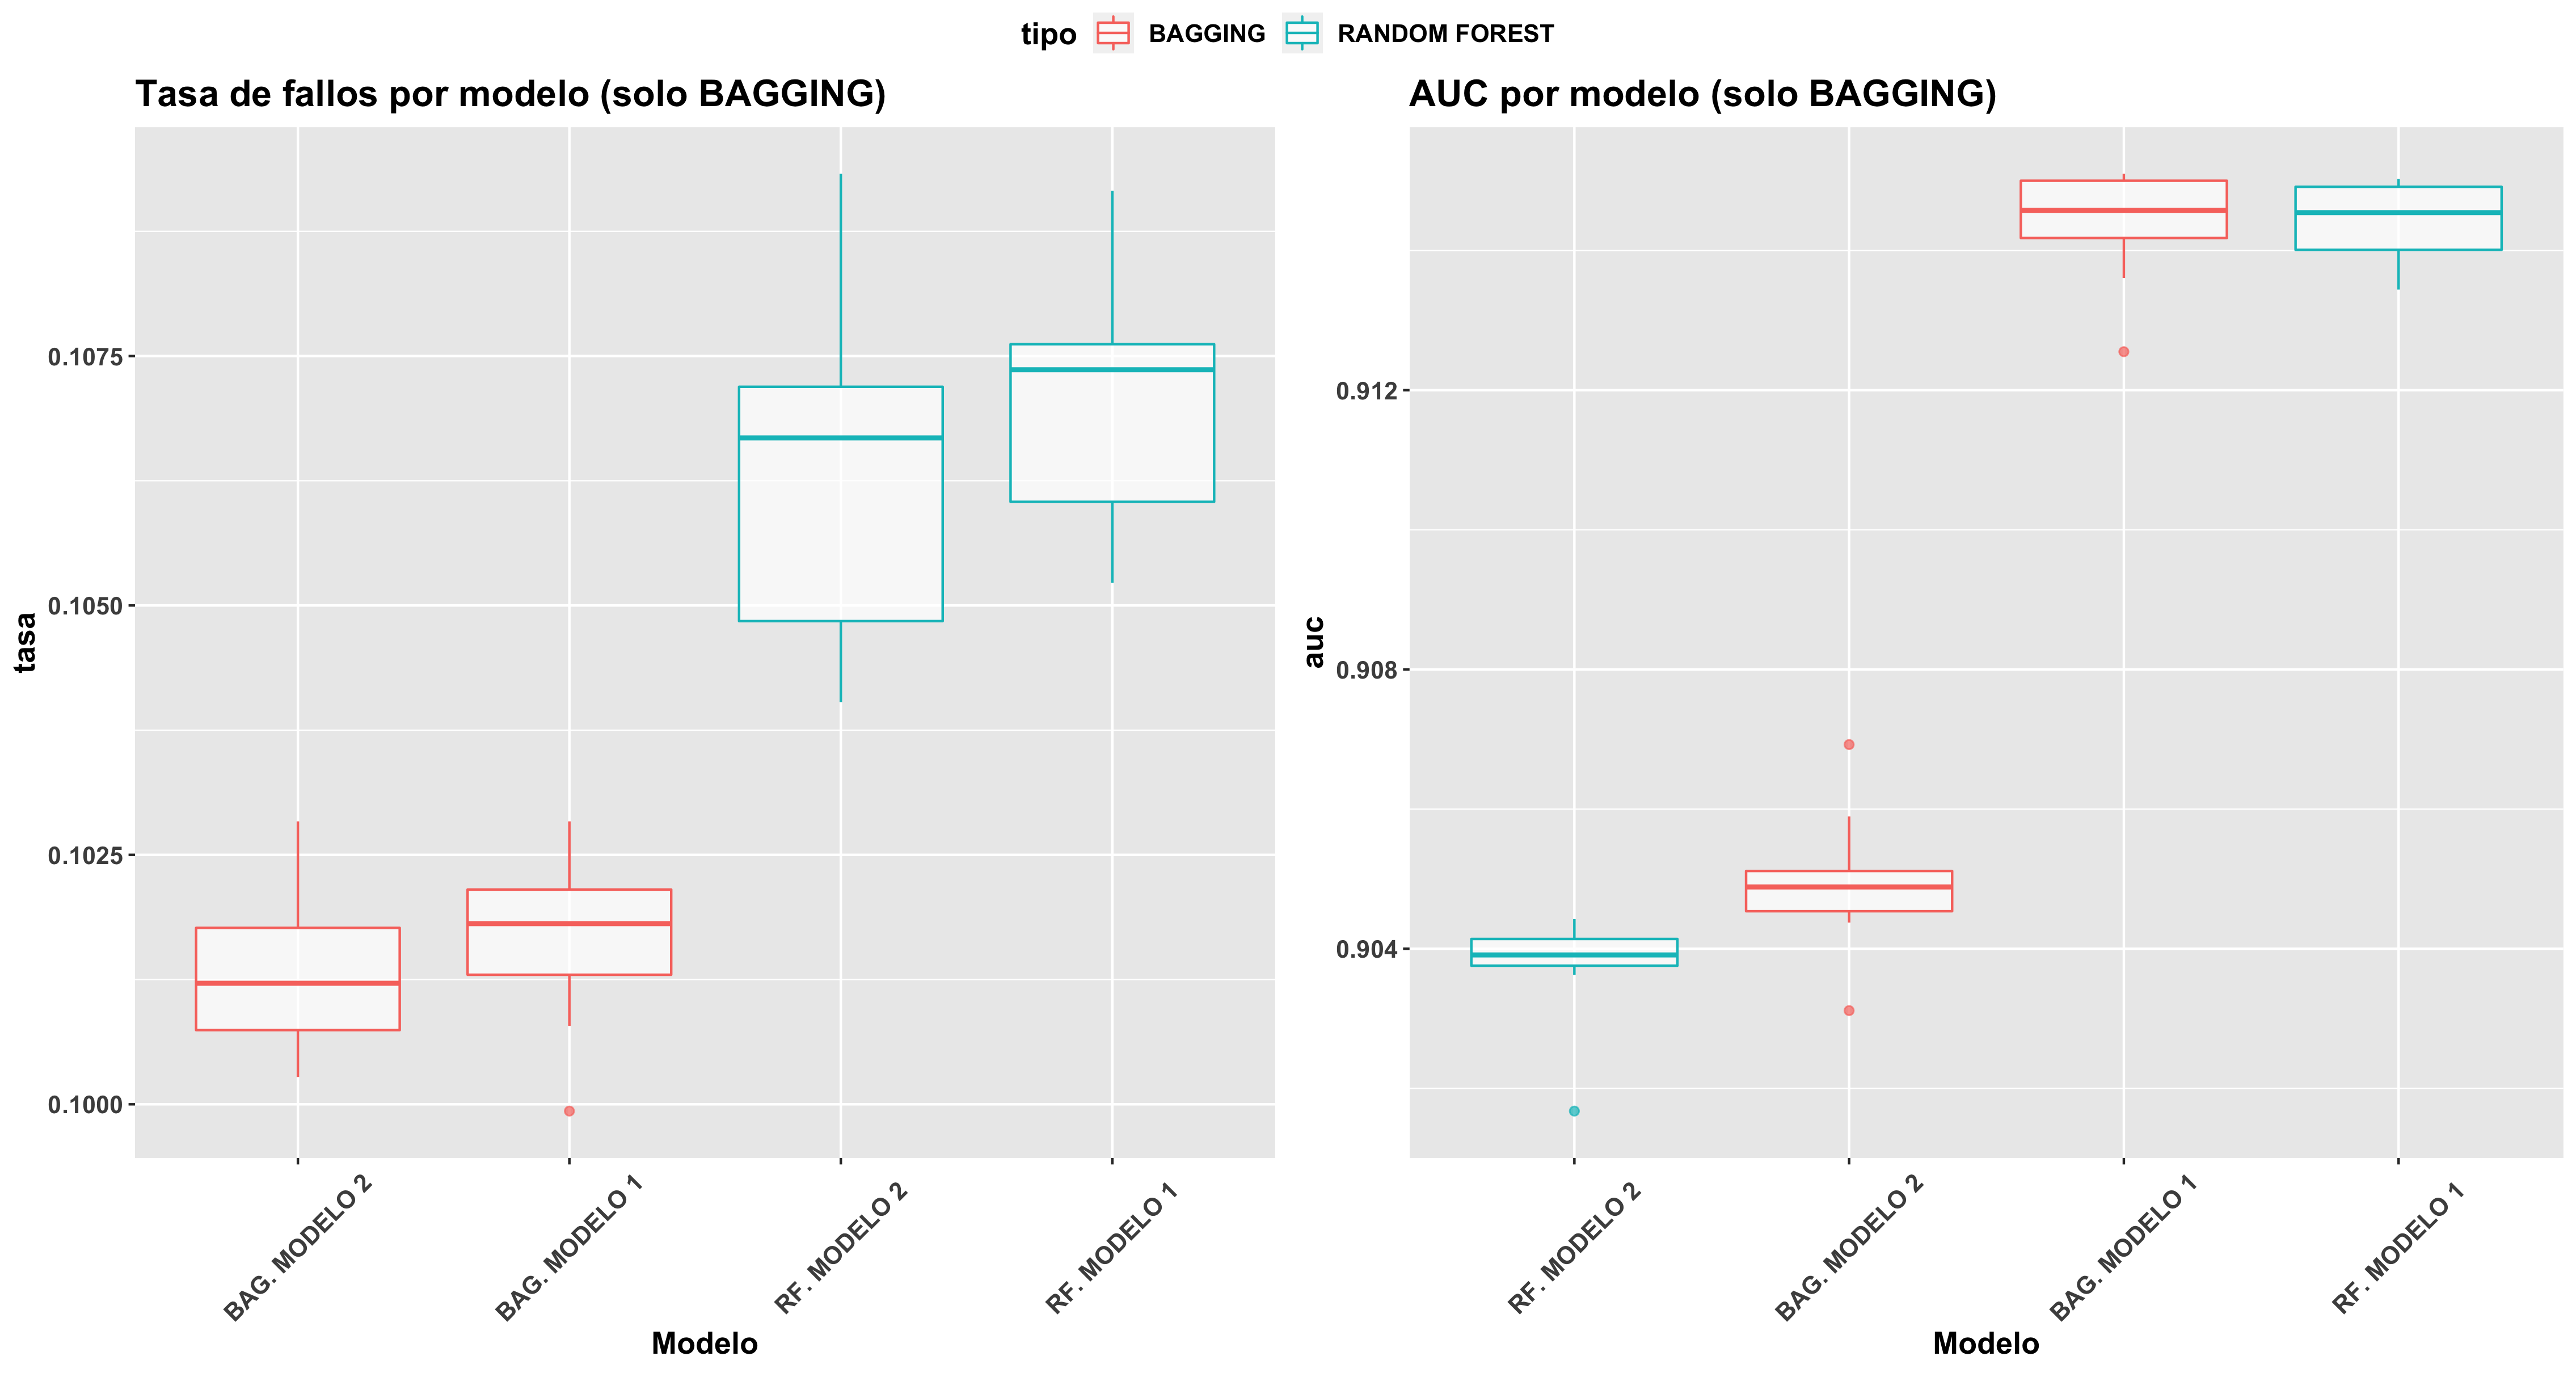
\includegraphics[width=0.99\linewidth,height=0.99\textheight,]{./charts/random_forest/comparacion_bagging_rf} 

}

\caption{Comparacion modelos bagging y rf}\label{fig:unnamed-chunk-105}
\end{figure}

Comprobamos que la diferencia entre ambos no es muy significativa, como
es el caso de la tasa de fallos, donde la escala del eje puede llevar a
engaño, ya que la diferencia entre ambos modelos es de apenas unas
milésimas (de 0.1000 - 0.1025 en el caso de \emph{bagging} a
0.1050-0.1075 en \emph{random forest}). Además, aunque la varianza en
este último parezca aumentar, dada la escala del eje no es tan
pronunciada.

De nuevo, no existe demasiada diferencia entre ambos \emph{sets} de
variables, tanto en tasa de fallos como en AUC, pese a la diferencia de
una variable \emph{input}.

\hypertarget{gradient-boosting}{%
\section{\texorpdfstring{9. \emph{Gradient
Boosting}}{9. Gradient Boosting}}\label{gradient-boosting}}

Hasta el momento, hemos comprobado como la variación en el
\emph{accuracy}, tasa de error o AUC con los ambos \emph{sets}
candidatos no resulta ser relevante, incluso en numerosas ocasiones los
parámetros finales acaban siendo los mismos para ambos candidatos. Por
tanto, de cara al resto de modelos como \emph{grandient boosting},
\emph{xgboost} o \emph{svm}, veamos si es posible poner en común un
mismo tuneo de hipérparametros para ambos \emph{sets}, en lugar de
``tunear'' por separado cada uno de ellos.

\hypertarget{tuneo-de-hipuxe9rparuxe1metros}{%
\subsection{9.1 Tuneo de
hipérparámetros}\label{tuneo-de-hipuxe9rparuxe1metros}}

En primer lugar, comenzando con el tuneo de los diferentes
hiperparámetrosm en ambos modelos, con tan solo cinco repeticiones:

\begin{enumerate}
\def\labelenumi{\arabic{enumi}.}
\tightlist
\item
  \emph{shrinkage}: parámetro de regularización.
\item
  \emph{n.minobsinnode}: tamaño máximo de nodos finales (parámetro
  encargado de medir la complejidad).
\item
  \emph{n.trees}: número de iteraciones (árboles).
\item
  \emph{bag.fraction}: fracción de observaciones del conjunto de
  entrenamiento seleccionadas aleatoriamente para la construcción del
  siguiente árbol.
\end{enumerate}

\begin{Shaded}
\begin{Highlighting}[]
\CommentTok{\#{-}{-} Ejemplo de tuneo con el primer set de variables}
\KeywordTok{set.seed}\NormalTok{(}\DecValTok{1234}\NormalTok{)}
\CommentTok{\#{-}{-} El valor maximo de shrinkage suele estar en torno a 0.2 (probamos con 0.3 y 0.4 tambien)}
\NormalTok{gbmgrid<{-}}\KeywordTok{expand.grid}\NormalTok{(}\DataTypeTok{shrinkage=}\KeywordTok{c}\NormalTok{(}\FloatTok{0.4}\NormalTok{,}\FloatTok{0.3}\NormalTok{,}\FloatTok{0.2}\NormalTok{,}\FloatTok{0.1}\NormalTok{,}\FloatTok{0.05}\NormalTok{,}\FloatTok{0.03}\NormalTok{,}\FloatTok{0.01}\NormalTok{,}\FloatTok{0.001}\NormalTok{),}
                     \DataTypeTok{n.minobsinnode=}\KeywordTok{c}\NormalTok{(}\DecValTok{5}\NormalTok{,}\DecValTok{10}\NormalTok{,}\DecValTok{20}\NormalTok{),}
                     \DataTypeTok{n.trees=}\KeywordTok{c}\NormalTok{(}\DecValTok{100}\NormalTok{,}\DecValTok{500}\NormalTok{,}\DecValTok{1000}\NormalTok{,}\DecValTok{5000}\NormalTok{),}
                     \DataTypeTok{interaction.depth=}\KeywordTok{c}\NormalTok{(}\DecValTok{2}\NormalTok{))}

\CommentTok{\#{-}{-} De momento, mantenemos bag.fraction a 1 (todas las observaciones)}
\NormalTok{control<{-}}\KeywordTok{trainControl}\NormalTok{(}\DataTypeTok{method=}\StringTok{"repeatedcv"}\NormalTok{,}\DataTypeTok{number=}\DecValTok{5}\NormalTok{,}\DataTypeTok{savePredictions =} \StringTok{"all"}\NormalTok{, }
                      \DataTypeTok{repeats=}\DecValTok{5}\NormalTok{,}\DataTypeTok{classProbs=}\OtherTok{TRUE}\NormalTok{)}
\NormalTok{gbm\_modelo1 <{-}}\StringTok{ }\KeywordTok{train}\NormalTok{(formula\_modelo\_}\DecValTok{1}\NormalTok{,}\DataTypeTok{data=}\NormalTok{surgical\_dataset,}
                     \DataTypeTok{method=}\StringTok{"gbm"}\NormalTok{,}\DataTypeTok{trControl=}\NormalTok{control,}\DataTypeTok{tuneGrid=}\NormalTok{gbmgrid,}
                     \DataTypeTok{distribution=}\StringTok{"bernoulli"}\NormalTok{, }\DataTypeTok{bag.fraction=}\DecValTok{1}\NormalTok{,}\DataTypeTok{verbose=}\OtherTok{FALSE}\NormalTok{)}
\end{Highlighting}
\end{Shaded}

\begin{figure}[h!]

{\centering \includegraphics[width=0.99\linewidth,height=0.99\textheight,]{./charts/gradient_boosting/05_gbm_hyperparameters_modelo1} 

}

\caption{Comparacion hiperparámetros gbm modelo 1}\label{fig:unnamed-chunk-107}
\end{figure}
\begin{figure}[h!]

{\centering \includegraphics[width=0.99\linewidth,height=0.99\textheight,]{./charts/gradient_boosting/05_gbm_hyperparameters_modelo2} 

}

\caption{Comparación hiperparámetros gbm modelo 2}\label{fig:unnamed-chunk-108}
\end{figure}

¿Qué sucede en ambos \emph{sets} de variables? En primer lugar,
analicemos las recomendaciones de \emph{caret} para ambos \emph{sets}:

\begin{verbatim}
Modelo 1: n.trees = 500,  shrinkage = 0.1,  n.minobsinnode = 20. Accuracy: 0.9055354
Modelo 2: n.trees = 5000, shrinkage = 0.01, n.minobsinnode = 20. Accuracy: 0.9039292
\end{verbatim}

En función de lo recomendado por el propio paquete, existe un contraste
entre ambos modelos: por un lado, con cinco variables \emph{input}
recomienda 500 iteraciones, un valor de regularización alto y
\emph{n.minobsinnode} alto (20), es decir, modelos más simples. Por el
contrario, con una variable \emph{input} menos, recomienda muchos más
árboles (5000) y un valor de regularización más bajo.

Desde un punto de vista numérico, con estos parámetros se han obtenido
el \emph{accuracy} máximo (incluso también por la estructura de
remuestreo, valor de la semilla, etc.). Sin embargo, ¿Es una
configuración óptima? O aún más importante ¿Podrían obtenerse resultados
similares con modelos más sencillos? Para responder a ambas preguntas,
\textbf{debemos analizar los posibles patrones que presenta el modelo en
ambos \emph{sets}}, de forma que podamos decantarnos por una opción
mucho más sencilla.

Concretamente, destacamos tres grandes patrones de comportamiento:

\begin{enumerate}
\def\labelenumi{\arabic{enumi}.}
\item
  Por un lado, \textbf{un bajo número de iteraciones (en torno a 100),
  junto con un valor de regularización alto ( \emph{shrinkage} superior
  o igual a 0.2-0.3, aproximadamente)}.
\item
  Por el contrario, también es posible obtener un máximo \emph{accuracy}
  \textbf{con un valor \emph{shrinkage} bajo (inferior a 0.1), pero con
  un elevado número de iteraciones, en torno a 500, 1000 o 5000}.
\item
  Además, el comportamiento de \emph{n.minobsinnode} en ambos
  \emph{sets} es el mismo tanto para un valor de 5, como de 10 o 20,
  \textbf{por lo que un valor alto (20) es una buena opción a
  decantarse: a un mayor valor \emph{n.minosinnode}, obtenemos modelos
  más simples y con menos posibilidad de sobreajuste}.
\end{enumerate}

En conclusión, \textbf{no es necesario tunear exageradamente el modelo
en ambos casos}, sino que aparentemente con un número de árboles bajo
(100), un valor de regularización alto (en torno a 0.2-0.3) y
\emph{n.minobsinnode} = 20 se obtienen de por sí buenos resultados, sin
necesidad de complicar aún más el modelo.

\hypertarget{estudio-del-early-stopping}{%
\subsubsection{\texorpdfstring{9.1.1 Estudio del \emph{Early
Stopping}}{9.1.1 Estudio del Early Stopping}}\label{estudio-del-early-stopping}}

Continuando con la línea anterior, para ambos \emph{set} de variables
\textbf{probamos a fijar \emph{n.minobsinnode} = 20 y \emph{shrinkage} =
0.2 y 0.3}, observando no solo qué número de iteraciones/árboles sería
adecuado utilizar, sino además si con un valor de regularización de 0.2
es suficiente o si aumentando su valor obtenemos mejores resultados, ya
que en el gráfico anterior se detectó un ligero ascenso en el valor de
\emph{accuracy} en 0.3 (normalmente el valor máximo suele ser 0.2):

\begin{figure}[h!]

{\centering \includegraphics[width=0.99\linewidth,height=0.99\textheight,]{./charts/gradient_boosting/05_early_stopping} 

}

\caption{Estudio Early Stopping Modelos 1 y 2}\label{fig:unnamed-chunk-109}
\end{figure}

En ambos \emph{sets}, \textbf{observamos que con 100 árboles se obtiene
un buen \emph{accuracy}}, mientras que a partir de 400-500 iteraciones,
el modelo comienza a sobreajustarse y, como consecuencia, disminuye su
precisión. Por otro lado, en relación con el parámetro \emph{shrinkage}
no existe apenas diferencia entre un valor 0.2 y 0.3, por lo que
\textbf{nos decantamos por 0.2}.

\hypertarget{estudio-de-bag.fraction}{%
\subsubsection{\texorpdfstring{9.1.2 Estudio de
\emph{bag.fraction}}{9.1.2 Estudio de bag.fraction}}\label{estudio-de-bag.fraction}}

Hasta el momento, hemos tuneado los modelos \emph{gbm} \textbf{con el
conjunto total de las observaciones, esto es, con \emph{bag.fraction} =
1}. Sin embargo, \emph{caret} por defecto \textbf{no sortea todas las
observaciones, sino que por defecto escoge el 50 \% aleatoriamente
(0.5)} \footnote{\emph{caret} emplea internamente el paquete \emph{gbm},
  cuyo valor \emph{bag.fraction} por defecto es 0.5.
  \url{https://cran.r-project.org/web/packages/gbm/gbm.pdf}}

Como consecuencia, sobre ambos \emph{sets} \textbf{estudiamos la
variabilidad del modelo con respecto a dicho parámetro}, aumentando a 10
el número de repeticiones para observar mejor su efecto. Dado que la
función \emph{cruzadagbmbin} nos dispone de dicho parámetro, se ha
incluido internamente en la función \emph{train} de \emph{caret}:

\begin{Shaded}
\begin{Highlighting}[]
\CommentTok{\#{-}{-} bag.fraction no se permite tunear desde expand.grid...}
\NormalTok{gbmgrid <{-}}\StringTok{ }\KeywordTok{expand.grid}\NormalTok{(}\DataTypeTok{n.minobsinnode=}\NormalTok{n.minobsinnode, }\DataTypeTok{shrinkage=}\NormalTok{shrinkage,}
                      \DataTypeTok{n.trees=}\NormalTok{n.trees, }\DataTypeTok{interaction.depth=}\NormalTok{interaction.depth)}
\CommentTok{\#{-}{-} Por lo que lo incluimos dentro de train  }
\NormalTok{gbm    <{-}}\StringTok{ }\KeywordTok{train}\NormalTok{(formu,}\DataTypeTok{data=}\NormalTok{databis, }\DataTypeTok{method=}\StringTok{"gbm"}\NormalTok{,}\DataTypeTok{trControl=}\NormalTok{control,}
                \DataTypeTok{bag.fraction=}\NormalTok{bag.fraction, }\DataTypeTok{tuneGrid=}\NormalTok{gbmgrid,}\DataTypeTok{distribution=}\StringTok{"bernoulli"}\NormalTok{,}
                \DataTypeTok{verbose=}\OtherTok{FALSE}\NormalTok{)}
\end{Highlighting}
\end{Shaded}

\begin{figure}[h!]

{\centering \includegraphics[width=0.99\linewidth,height=0.99\textheight,]{./charts/gradient_boosting/05_gbm_bag_fraction} 

}

\caption{Estudio bag.fraction modelos 1 y 2}\label{fig:unnamed-chunk-111}
\end{figure}

En un primer análisis, la diferencia entre \emph{bag.fraction} = 0.5 y
\emph{bag.fraction} = 1 es pequeña, ya que tanto en sesgo como en
varianza presentan resultados similares, salvo en la tasa de fallos
donde aumenta ligeramente, pero no demasiado dada la escala de los ejes
(por ejemplo, en el modelo 1 la varianza se sitúa entre 0.099 y 0.104,
considerando los \emph{outliers}). Por tanto, \textbf{no existe apenas
diferencia entre utilizar el 100 \% de las observaciones y tan solo el
50 \%}, por lo que podemos mantener dicho parámetro por defecto en
\emph{bag.fraction}.

\textbf{RESUMEN \emph{gradient boosting}}:

\begin{enumerate}
\def\labelenumi{\arabic{enumi}.}
\tightlist
\item
  modelos 1 y 2: \emph{n.trees} = 100, \emph{shrinkage} = 0.2,
  \emph{n.minobsinnode} = 20 y \emph{bag.fraction} = 0.5.
\end{enumerate}

\hypertarget{comparaciuxf3n-final-3}{%
\subsection{9.2 Comparación final}\label{comparaciuxf3n-final-3}}

A continuación, con los modelos obtenidos realizamos la predicción sobre
el conjunto \emph{test}:

\begin{verbatim}
##                 modelo precision sensibilidad especificidad valor_pred_pos
## 1 Modelo 1 (BIC TOP 5)    0.9030       0.9149        0.9003         0.6731
## 2     Modelo 2 (top 4)    0.9052       0.9264        0.9006         0.6731
##   valor_pred_neg
## 1         0.9792
## 2         0.9823
\end{verbatim}

Como podemos comprobar, \emph{gradient boosting} se sitúa prácticamente
en la misma línea que el resto de modelos basados en árbol: \textbf{alta
precisión, sensibilidad, especificidad y valor predictivo negativo, pero
con un valor predictivo positivo menor, en torno al 67 \%}:

\begin{figure}[h!]

{\centering \includegraphics[width=0.99\linewidth,height=0.99\textheight,]{./charts/comparativas/05_log_avnnet_bagging_rf_gbm_tasa} 

}

\caption{Comparacion tasa fallos log-avnnet-bagging-rf-gbm}\label{fig:unnamed-chunk-113}
\end{figure}
\begin{figure}[h!]

{\centering \includegraphics[width=0.99\linewidth,height=0.99\textheight,]{./charts/comparativas/05_log_avnnet_bagging_rf_gbm_auc} 

}

\caption{Comparacion AUC log-avnnet-bagging-rf-gbm}\label{fig:unnamed-chunk-114}
\end{figure}

De hecho, aunque la tasa de fallos en \emph{gradient boosting} sea
ligeramente menor, \textbf{modelos como \emph{random forest} o
\emph{bagging} continuan siendo una mejor alternativa}.

\hypertarget{support-vector-machines}{%
\section{\texorpdfstring{10. \emph{Support Vector
Machines}}{10. Support Vector Machines}}\label{support-vector-machines}}

\hypertarget{svm-lineal}{%
\subsection{10.1 SVM Lineal}\label{svm-lineal}}

A continuación, continuamos con los modelos \emph{svm}, comenzando por
el \emph{kernel} más sencillo: el lineal, del cual solo necesitamos
tunear el parámetro de regularización \textbf{C} (por el momento,
empleamos 5 repeticiones):

\begin{Shaded}
\begin{Highlighting}[]
\CommentTok{\#{-}{-} Probamos desde C = 0.01 hasta C = 10}
\NormalTok{C\_binaria <{-}}\StringTok{ }\KeywordTok{expand.grid}\NormalTok{(}\DataTypeTok{C=}\KeywordTok{c}\NormalTok{(}\FloatTok{0.01}\NormalTok{,}\FloatTok{0.05}\NormalTok{,}\FloatTok{0.1}\NormalTok{,}\FloatTok{0.2}\NormalTok{,}\FloatTok{0.5}\NormalTok{,}\DecValTok{1}\NormalTok{,}\DecValTok{2}\NormalTok{,}\DecValTok{5}\NormalTok{,}\DecValTok{10}\NormalTok{))}

\CommentTok{\#{-}{-} Ejemplo con el primer set de variables (5 variables input)}
\KeywordTok{cruzadaSVMbin}\NormalTok{(}\DataTypeTok{data=}\NormalTok{surgical\_dataset, }\DataTypeTok{vardep=}\NormalTok{target,}
                           \DataTypeTok{listconti =}\NormalTok{ var\_modelo1, }\DataTypeTok{listclass=}\KeywordTok{c}\NormalTok{(}\StringTok{""}\NormalTok{),}
                           \DataTypeTok{grupos=}\DecValTok{5}\NormalTok{,}\DataTypeTok{sinicio=}\DecValTok{1234}\NormalTok{,}\DataTypeTok{repe=}\DecValTok{5}\NormalTok{,}\DataTypeTok{C=}\NormalTok{C\_binaria)}
\end{Highlighting}
\end{Shaded}

\begin{figure}[h!]

{\centering \includegraphics[width=0.99\linewidth,height=0.99\textheight,]{./charts/SVM/06_svm_lineal_modelo1_2} 

}

\caption{Distribución SVM Lineal Modelos 1 y 2}\label{fig:unnamed-chunk-116}
\end{figure}

\begin{verbatim}
Recomendado por caret
Modelo 1: C = 0.01. Accuracy: 0.7746143
Modelo 2: C = 0.01. Accuracy: 0.7466688
\end{verbatim}

A diferencia del resto de modelos no lineales, con el primer \emph{set}
de variables (5 variables \emph{input} incluyendo \emph{ccsMort30Rate}),
obtenemos un \emph{accuracy} en torno al 77 \%, mientras que con tan
solo 4 variables desciende al 74 \%, de nuevo un indicativo de la
relación lineal de dicha variable con la variable objetivo. Pese a ello,
\textbf{los modelos basados en árbol o \emph{boosting} continuan siendo
mejor en términos de \emph{accuracy} (89-90 \%)}.

En relación con la constante C, dada la escala de los ejes \textbf{no se
aprecia una diferencia relevante entre los diferentes valores}, ya que
apenas varían en unas milésimas. Sin embargo, si se tuviera que indica
un posible patrón, diríamos que a medida que se reduce la constance C,
aumenta ligeramente el \emph{accuracy}. Podríamos incluso probar a
reducir aún más el parámetro de regularización:

\begin{Shaded}
\begin{Highlighting}[]
\CommentTok{\#{-}{-} Probamos a reducir C entre 0.1 y 0.001}
\NormalTok{C\_binaria <{-}}\StringTok{ }\KeywordTok{expand.grid}\NormalTok{(}\DataTypeTok{C=}\KeywordTok{c}\NormalTok{(}\FloatTok{0.001}\NormalTok{,}\FloatTok{0.005}\NormalTok{,}\FloatTok{0.01}\NormalTok{))}
\end{Highlighting}
\end{Shaded}

Pero tan solo aumenta en 0.0001 en ambos \emph{sets}:

\begin{verbatim}
Modelo 1: C: 0.01 -> 0.7746143 ; C: 0.001 -> 0.7749898
Modelo 2: C: 0.01 -> 0.7466688 ; C: 0.001 -> 0.7749898
\end{verbatim}

Por tanto, y dado que la diferencia no es muy significativa, \textbf{nos
decantamos por el máximo \emph{accuracy}, correspondiente con C = 0.01},
recomendado por \emph{caret}, un valor no demasiado alto, lo que se
traduce en un menor riesgo por sobreajuste (márgenes de separación mucho
mayores).

\hypertarget{svm-polinomial}{%
\subsection{10.2 SVM Polinomial}\label{svm-polinomial}}

A continuación, proseguimos con el \emph{kernel} polinomial,
\textbf{tuneando tanto la constante C de regularización como la escala}
(nuevamente, con cinco repeticiones):

\textbf{NOTA: dado que los polinomios de grado 3 tardaban demasiado
tiempo en procesar (incluso con una sola repetición +
\emph{doParallel}), se ha utilizado únicamente grado 2}.

\begin{Shaded}
\begin{Highlighting}[]
\CommentTok{\#{-}{-} Probamos con C desde 0.01 hasta 10}
\NormalTok{C\_poly      <{-}}\StringTok{ }\KeywordTok{c}\NormalTok{(}\FloatTok{0.01}\NormalTok{, }\FloatTok{0.05}\NormalTok{, }\FloatTok{0.1}\NormalTok{, }\FloatTok{0.2}\NormalTok{, }\FloatTok{0.5}\NormalTok{, }\DecValTok{1}\NormalTok{, }\DecValTok{2}\NormalTok{, }\DecValTok{5}\NormalTok{, }\DecValTok{10}\NormalTok{)}
\NormalTok{degree\_poly <{-}}\StringTok{ }\KeywordTok{c}\NormalTok{(}\DecValTok{2}\NormalTok{)}
\CommentTok{\#{-}{-} Probamos desde una escala pequeña (0.1) hasta 5}
\NormalTok{scale\_poly  <{-}}\StringTok{ }\KeywordTok{c}\NormalTok{(}\FloatTok{0.1}\NormalTok{, }\FloatTok{0.5}\NormalTok{, }\DecValTok{1}\NormalTok{, }\DecValTok{2}\NormalTok{, }\DecValTok{5}\NormalTok{)}

\CommentTok{\#{-}{-} Ejemplo con el primer set de variables (5 variables input)}
\NormalTok{svm\_pol\_}\DecValTok{1}\NormalTok{ <{-}}\StringTok{ }\KeywordTok{cruzadaSVMbinPoly}\NormalTok{(}\DataTypeTok{data=}\NormalTok{surgical\_dataset, }\DataTypeTok{vardep=}\NormalTok{target,}
                               \DataTypeTok{listconti =}\NormalTok{ var\_modelo1, }\DataTypeTok{listclass=}\KeywordTok{c}\NormalTok{(}\StringTok{""}\NormalTok{),}
                               \DataTypeTok{grupos=}\DecValTok{5}\NormalTok{,}\DataTypeTok{sinicio=}\DecValTok{1234}\NormalTok{,}\DataTypeTok{repe=}\DecValTok{5}\NormalTok{,}\DataTypeTok{C =}\NormalTok{ C\_poly,}
                               \DataTypeTok{degree =}\NormalTok{ degree\_poly, }\DataTypeTok{scale =}\NormalTok{ scale\_poly)}
\end{Highlighting}
\end{Shaded}

\begin{figure}[h!]

{\centering \includegraphics[width=0.99\linewidth,height=0.99\textheight,]{./charts/SVM/06_svm_poly_modelo1_2} 

}

\caption{Distribución SVM Polinomial Modelos 1 y 2 (I)}\label{fig:unnamed-chunk-119}
\end{figure}

\begin{verbatim}
Recomendado por caret
Modelo 1: C = 5   ; degree = 2; scale = 0.1. Accuracy: 0.7766301
Modelo 2: C = 0.01; degree = 2; scale = 0.1. Accuracy: 0.7766992
\end{verbatim}

En base a la respuesta del paquete \emph{caret}, con el primer
\emph{set} recomienda una escala en torno a 0.1 y una constance C alta
(5), mientras que en el caso del segundo \emph{set} de variables, la
constante C recomendada es más baja, en torno a 0.01. No obstante, y
dado que \textbf{no podemos dejarnos llevar por valores puntuales (pues
puede conducir al sobreajuste), analicemos los patrones existentes}:

\begin{enumerate}
\def\labelenumi{\arabic{enumi}.}
\item
  En el caso del primer \emph{set} de variables, nos encontramos con dos
  posibles extremos: \textbf{o bien una constante C alta (entre 5 y 10)
  y una escala moderada/pequeña (en torno a 0.1-0.5-1) o una constante C
  pequeña y una escala mayor (1, 2 o 5)}.
\item
  En el segundo \emph{set}, por otro lado, \textbf{llama la atención
  modelos con una constante C pequeña (menor a 0.01) y una escala baja
  (0.1-0.5, principalmente)}.
\end{enumerate}

Por tanto, analicemos si mejoran los resultados en caso de, en el primer
\emph{set}, aumentar la constante C a 15 y 20, así como disminuirlo a
0.005 y 0.001. Por otro lado, probamos también a reducir C a 0.005 y
0.001 en el segundo \emph{set} de variables:

\begin{figure}[h!]

{\centering \includegraphics[width=0.99\linewidth,height=0.99\textheight,]{./charts/SVM/polinomica/svm_polinomial_parte2} 

}

\caption{Distribución SVM Polinomial Modelos 1 y 2 (II)}\label{fig:unnamed-chunk-120}
\end{figure}

\begin{enumerate}
\def\labelenumi{\arabic{enumi}.}
\tightlist
\item
  En el caso del primer \emph{set}, pese a reducir o aumentar la
  constante C, el valor de \emph{accuracy} se mantiene en torno a 0.77.
  Por tanto, y dado que la diferencia no es muy significativa entre un
  valor C alto y pequeño, \textbf{podemos decantarnos por un valor en
  torno a 0.5 (moderado-bajo), así como una escala de 1}, aunque
  \emph{caret} nos recomiende un valor C = 5, de forma que los márgenes
  de separación entre ambas clases es mayor, obteniendo un modelo más
  ``general''.
\end{enumerate}

De nuevo, \textbf{la decision esta basada por patrones y no en valores
puntuales}, por lo que empleando otra semilla y con otros valores
training los parametros serán ``aproximadamente'' similares, aunque no
iguales. Por tanto, dado que la diferencia entre un modelo SVM más
ajustado (C = 5) y un modelo más general (C = 0.5) es ínfima.

\begin{enumerate}
\def\labelenumi{\arabic{enumi}.}
\setcounter{enumi}{1}
\tightlist
\item
  Por otro lado, en relación con el segundo \emph{set}, habiendo
  disminuido el valor C hasta 0.001-0.005, no ha hecho aumentar en gran
  medida el resultado. Por tanto, dado que con un valor C pequeño no
  solo obtenemos un mayor margen de separación (maniobrabilidad), sino
  además el mismo \emph{accuracy} que el de un modelo más ``estricto''
  en la separación, \textbf{nos decantamos por la opción de
  \emph{caret}}: C pequeño (0.01) y escala pequeña (0.1).
\end{enumerate}

\hypertarget{svm-rbf}{%
\subsection{10.3 SVM RBF}\label{svm-rbf}}

Finalizando con el \emph{kernel} radial, comenzando tuneando los dos
parámetros principales: C y \(\sigma\):

\begin{Shaded}
\begin{Highlighting}[]
\CommentTok{\#{-}{-} Probamos con C entre 0.01 y 10}
\NormalTok{C\_rbf      <{-}}\StringTok{ }\KeywordTok{c}\NormalTok{(}\FloatTok{0.01}\NormalTok{,}\FloatTok{0.05}\NormalTok{,}\FloatTok{0.1}\NormalTok{,}\FloatTok{0.2}\NormalTok{,}\FloatTok{0.5}\NormalTok{,}\DecValTok{1}\NormalTok{,}\DecValTok{2}\NormalTok{,}\DecValTok{5}\NormalTok{,}\DecValTok{10}\NormalTok{)}
\NormalTok{sigma\_rbf  <{-}}\StringTok{ }\KeywordTok{c}\NormalTok{(}\FloatTok{0.1}\NormalTok{, }\FloatTok{0.5}\NormalTok{, }\DecValTok{1}\NormalTok{, }\DecValTok{2}\NormalTok{, }\DecValTok{5}\NormalTok{, }\DecValTok{10}\NormalTok{)}

\CommentTok{\#{-}{-} Ejemplo con el primer set variables}
\NormalTok{svm\_rbf\_}\DecValTok{1}\NormalTok{ <{-}}\StringTok{ }\KeywordTok{cruzadaSVMbinRBF}\NormalTok{(}\DataTypeTok{data=}\NormalTok{surgical\_dataset, }\DataTypeTok{vardep=}\NormalTok{target,}
                              \DataTypeTok{listconti =}\NormalTok{ var\_modelo1, }\DataTypeTok{listclass=}\KeywordTok{c}\NormalTok{(}\StringTok{""}\NormalTok{),}
                              \DataTypeTok{grupos=}\DecValTok{5}\NormalTok{,}\DataTypeTok{sinicio=}\DecValTok{1234}\NormalTok{,}\DataTypeTok{repe=}\DecValTok{5}\NormalTok{,}\DataTypeTok{C =}\NormalTok{ C\_rbf,}
                              \DataTypeTok{sigma =}\NormalTok{ sigma\_rbf, }\DataTypeTok{label =} \StringTok{"Modelo 1"}\NormalTok{)}
\end{Highlighting}
\end{Shaded}

\begin{figure}[h!]

{\centering \includegraphics[width=0.99\linewidth,height=0.99\textheight,]{./charts/SVM/svm_rbf_modelos1_2} 

}

\caption{Distribución SVM RBF Modelos 1 y 2 (I)}\label{fig:unnamed-chunk-122}
\end{figure}

\begin{verbatim}
Recomendado por caret
Modelo 1: C = 1   ; sigma = 5 ; Accuracy: 0.8422943
Modelo 2: C = 1   ; sigma = 5 ; Accuracy: 0.8726666
\end{verbatim}

En base a los resultados devueltos por \emph{caret}, para ambos
\emph{sets} de variables recomienda una constante C pequeña/moderada
(1), así como un valor \(\sigma = 5\). No obstante, y dado que se tratan
de valores puntuales, analicemos los patrones existentes:

\begin{enumerate}
\def\labelenumi{\arabic{enumi}.}
\item
  En el caso del primer \emph{set}, \textbf{los modelos con mayor
  \emph{accuracy} presentan un valor sigma alto (en torno a 5-10 aumenta
  hasta 0.83)}. En relación al valor C, prácticamente con cualquier
  valor el \emph{accuracy} se sitúa en torno a 0.86-0.87, alcanzando su
  punto máximo en C = 1. Es decir, \textbf{no es necesario un valor C
  alto (márgenes de separación más pequeños), ya que a partir de C = 2,
  5, el \emph{accuracy} comienza a disminuir}. Por otro lado, otro
  posible patrón de comportamiento sería con un valor \emph{sigma} menor
  (2) y C alto (a partir de 5-10), donde comienza a aumentar el
  \emph{accuracy}.
\item
  En el caso del segundo modelo, el comportamiento es bastante similar:
  \textbf{o bien escogemos valores \emph{sigma} altos (5-10) y C no
  demasiado alto (menor a 1), o bien un valor \emph{sigma} menor (2) y
  una constante C alta (en torno a 5, 10)}.
\end{enumerate}

En ambos \emph{sets}, podemos comprobar cómo evoluciona el modelo si
aumentamos el valor de C con \emph{sigma} = 2, dado que a simple vista
comienza a aumentar conforme incrementamos C (de 0.775 a 0.875):

\begin{figure}[h!]

{\centering \includegraphics[width=0.99\linewidth,height=0.99\textheight,]{./charts/SVM/svm_rbf_modelos1_2_aumentando_C} 

}

\caption{Distribución SVM RBF Modelos 1 y 2 (II)}\label{fig:unnamed-chunk-123}
\end{figure}

Incluso aumentando \emph{C}, se obtienen prácticamente los mismos
resultados que con un \emph{sigma} y C menor.

En conclusión, para ambos \emph{sets} de variables \textbf{nos
decantamos por un valor \emph{sigma} alto (escogemos 5), y una constante
C no demasiado alta, entre 0.5 y 1}:

\begin{verbatim}
Recomendado por caret
Modelo 1: C = 1   ; sigma = 5 ; Accuracy: 0.8422943
          C = 0.5 ; sigma = 5 ; Accuracy: 0.8415420

Modelo 2: C = 1   ; sigma = 5 ; Accuracy: 0.8726666
          C = 0.5 ; sigma = 5 ; Accuracy: 0.8711983
\end{verbatim}

Dado que la diferencia entre \emph{C} = 1 y \emph{C} = 0.5 no es muy
relevante (aunque \emph{caret} recomiende 1), resulta indiferente
escoger uno de ellos (por ejemplo, escogemos 0.5).

\textbf{RESUMEN \emph{SVM Lineal}}:

\begin{enumerate}
\def\labelenumi{\arabic{enumi}.}
\tightlist
\item
  modelos 1 y 2: \emph{C} = 0.01.
\end{enumerate}

\textbf{RESUMEN \emph{SVM Polinomial}}:

\begin{enumerate}
\def\labelenumi{\arabic{enumi}.}
\tightlist
\item
  modelo 1: \emph{C} = 0.01 ; \emph{scale} = 0.1.
\item
  modelo 2: \emph{C} = 0.5 ; \emph{scale} = 1.
\end{enumerate}

\textbf{RESUMEN \emph{SVM RBF}}:

\begin{enumerate}
\def\labelenumi{\arabic{enumi}.}
\tightlist
\item
  modelo 1: \emph{C} = 0.5 ; \emph{sigma} = 5.
\item
  modelo 2: \emph{C} = 0.5 ; \emph{sigma} = 5.
\end{enumerate}

\hypertarget{comparaciuxf3n-modelos-svm}{%
\subsection{10.4 Comparación modelos
SVM}\label{comparaciuxf3n-modelos-svm}}

Una vez elaborados los modelos, \textbf{empleando validación cruzada
repetida de 5 grupos y 10 repeticiones, analizamos tanto la tasa de
fallos como el AUC (en ambos \emph{sets} de variables)}:

\begin{figure}[h!]

{\centering \includegraphics[width=0.99\linewidth,height=0.99\textheight,]{./charts/SVM/comparacion_svm} 

}

\caption{Comparación tasa de fallos y AUC modelos SVM}\label{fig:unnamed-chunk-124}
\end{figure}

Sin duda alguna, \textbf{la mejor alternativa tanto en tasa de fallos
como en AUC es el modelo SVM con \emph{kernel} radial (RBF)}. De hecho,
quisiera remarcar dos detalles fundamentales, relacionados con los
\emph{sets} de variables:

\begin{enumerate}
\def\labelenumi{\arabic{enumi}.}
\item
  Por un lado, en relación con el \emph{kernel} lineal,
  \textbf{observamos una considerable diferencia entre el primer
  \emph{set} con cinco variables (junto con \emph{ccsMort30Rate}) y el
  segundo \emph{set}, tanto en AUC, sesgo y varianza}: incluyendo dicha
  variable (relación lineal), el modelo mejora hasta 0.74-0.75 de AUC,
  aproximadamente, además de reducir la tasa de error hasta 0.22 (a
  diferencia del primer \emph{set}, que alcanza 0.26).
\item
  Por el contrario, con el \emph{kernel} radial, añadir dicha variable
  perjudica al modelo en cuanto a la tasa de fallos (de 0.16 con cinco
  variables a 0.12-0.13 con tan solo cuatro), aunque en AUC se mantienen
  prácticamente idénticos.
\end{enumerate}

Por otro lado, \textbf{analicemos las predicciones obtenidas con el
conjunto \emph{test}}:

\textbf{SVM Lineal}:

\begin{verbatim}
##                 modelo precision sensibilidad especificidad valor_pred_pos
## 1 Modelo 1 (BIC TOP 5)     0.789      0.65844       0.80678        0.31733
## 2     Modelo 2 (top 4)     0.549      0.49980       0.76550        0.17310
##   valor_pred_neg
## 1         0.9454
## 2         0.7823
\end{verbatim}

\textbf{SVM Polinomial}:

\begin{verbatim}
##                 modelo precision sensibilidad especificidad valor_pred_pos
## 1 Modelo 1 (BIC TOP 5)    0.7940      0.71977       0.80205        0.28304
## 2     Modelo 2 (top 4)    0.7826      0.63188       0.80316        0.30453
##   valor_pred_neg
## 1        0.96345
## 2        0.94116
\end{verbatim}

\textbf{SVM RBF}:

\begin{verbatim}
##                 modelo precision sensibilidad especificidad valor_pred_pos
## 1 Modelo 1 (BIC TOP 5)    0.8517       0.8000        0.8622         0.5396
## 2     Modelo 2 (top 4)    0.8804       0.8897        0.8786         0.5935
##   valor_pred_neg
## 1         0.9553
## 2         0.9756
\end{verbatim}

Al igual que en la comparación, con el conjunto \emph{test} \textbf{los
modelos SVM RBF resultan ser claramente los ganadores}, aunque con unos
porcentajes inferiores con respecto a los modelos basados en árbol o
\emph{gradient boosting}:

\begin{figure}[h!]

{\centering \includegraphics[width=0.99\linewidth,height=0.99\textheight,]{./charts/comparativas/06_log_avnnet_bagging_rf_gbm_svm_tasa} 

}

\caption{Comparacion tasa fallos log-avnnet-bagging-rf-gbm-svm}\label{fig:unnamed-chunk-128}
\end{figure}
\begin{figure}[h!]

{\centering \includegraphics[width=0.99\linewidth,height=0.99\textheight,]{./charts/comparativas/06_log_avnnet_bagging_rf_gbm_svm_auc} 

}

\caption{Comparacion AUC log-avnnet-bagging-rf-gbm-svm}\label{fig:unnamed-chunk-129}
\end{figure}

Antes de continuar con \emph{XGboost} y Ensamblado, debemos detenernos a
analizar si realmente es necesario continuar con ambos \emph{sets} de
variables o no. A lo largo de la práctica (logística, redes, modelos
basados en árbol, \emph{boosting}, svm) se ha podido comprobar que la
diferencia entre ambos candidatos, por tan solo una variable
\emph{input}, no ha sido especialmente relevante, pese a lo observado en
la regresión logística donde si existía cierta diferencia entre ambos.

Por tanto, de cara a \emph{XGboost} pero especialmente a los modelos de
Ensamblado \textbf{continuaremos con únicamente con el segundo
\emph{set} de variables \emph{input} (4 variables), a excepción del
modelo \emph{svm} lineal, donde utilizaremos el modelo obtenido con el
primer \emph{set}}.

\hypertarget{xgboost}{%
\section{11. XGboost}\label{xgboost}}

\hypertarget{tuneo-de-hiperparuxe1metros}{%
\subsection{11.1 Tuneo de
hiperparámetros}\label{tuneo-de-hiperparuxe1metros}}

En primer lugar, debemos recordar los parámetros a tunear en un modelo
\emph{XGboost}:

\begin{enumerate}
\def\labelenumi{\arabic{enumi}.}
\item
  \emph{min\_child\_weight}: número de observaciones mínimas en el nodo
  final. Similar a \emph{n.minobsinnnode} de \emph{gbm}.
\item
  \emph{eta}: parámetro de regularización.
\item
  \emph{rounds}: número de iteraciones.
\item
  \emph{max\_depth}: profundidad máxima de los árboles.
\item
  \emph{gamma}: constante de regularización (lo mantenemos a 0).
\item
  \emph{colsample\_bytree}: porcentaje de sorteo de variables en cada
  árbol (lo mantenemos a 1).
\item
  \emph{subsample}: sorteo de observaciones antes de cada árbol (lo
  mantenemos a 1).
\end{enumerate}

\begin{Shaded}
\begin{Highlighting}[]
\NormalTok{xgbmgrid <{-}}\StringTok{ }\KeywordTok{expand.grid}\NormalTok{(}\DataTypeTok{min\_child\_weight=}\KeywordTok{c}\NormalTok{(}\DecValTok{5}\NormalTok{,}\DecValTok{10}\NormalTok{,}\DecValTok{20}\NormalTok{),}
                        \DataTypeTok{eta=}\KeywordTok{c}\NormalTok{(}\FloatTok{0.1}\NormalTok{,}\FloatTok{0.05}\NormalTok{,}\FloatTok{0.03}\NormalTok{,}\FloatTok{0.01}\NormalTok{,}\FloatTok{0.001}\NormalTok{), }
                        \DataTypeTok{nrounds=}\KeywordTok{c}\NormalTok{(}\DecValTok{100}\NormalTok{,}\DecValTok{500}\NormalTok{,}\DecValTok{1000}\NormalTok{,}\DecValTok{5000}\NormalTok{),}
                        \DataTypeTok{max\_depth=}\DecValTok{6}\NormalTok{,}\DataTypeTok{gamma=}\DecValTok{0}\NormalTok{,}
                        \DataTypeTok{colsample\_bytree=}\DecValTok{1}\NormalTok{,}\DataTypeTok{subsample=}\DecValTok{1}\NormalTok{)}

\CommentTok{\#{-}{-} Probamos al comienzo con 5 repeticiones}
\KeywordTok{set.seed}\NormalTok{(}\DecValTok{1234}\NormalTok{)}
\NormalTok{control<{-}}\KeywordTok{trainControl}\NormalTok{(}\DataTypeTok{method =} \StringTok{"repeatedcv"}\NormalTok{,}\DataTypeTok{number=}\DecValTok{5}\NormalTok{,}\DataTypeTok{repeats =} \DecValTok{5}\NormalTok{,}
                      \DataTypeTok{savePredictions =} \StringTok{"all"}\NormalTok{,}\DataTypeTok{classProbs=}\OtherTok{TRUE}\NormalTok{)}

\NormalTok{xgbm\_ <{-}}\StringTok{ }\KeywordTok{train}\NormalTok{(formula\_modelo2,}\DataTypeTok{data=}\NormalTok{surgical\_dataset,}
               \DataTypeTok{method=}\StringTok{"xgbTree"}\NormalTok{,}\DataTypeTok{trControl=}\NormalTok{control,}
               \DataTypeTok{tuneGrid=}\NormalTok{xgbmgrid,}\DataTypeTok{verbose=}\OtherTok{FALSE}\NormalTok{)}
\end{Highlighting}
\end{Shaded}

\begin{figure}[h!]

{\centering \includegraphics[width=0.99\linewidth,height=0.99\textheight,]{./charts/xgboost/tuneo_xgboost_modelo2} 

}

\caption{Tuneo hiperparámetros XGboost}\label{fig:unnamed-chunk-131}
\end{figure}

De los gráficos anteriores, \textbf{se deduce que se debe tomar un valor
\emph{eta} alto (en torno a 0.1) y pocas iteraciones, alrededor de 100}.
Además, si nos fijamos en la escala de los ejes, \textbf{no existe
demasiada diference entre un valor \emph{min\_child\_weight} bajo (5) y
alto (20)}, tan solo de apenas unas décimas (0.90 y 0.89,
respectivamente). Por tanto, escogemos un valor de 20 al ser las
diferencias tan pequeñas, permitiendo con ello modelos más simples y con
menos sobreajuste.

\hypertarget{estudio-early-stopping}{%
\subsection{\texorpdfstring{11.2 Estudio \emph{Early
Stopping}}{11.2 Estudio Early Stopping}}\label{estudio-early-stopping}}

A continuación, probamos a fijar algunos parámetros para analizar cómo
evoluciona el modelo en función del número de iteraciones:

\begin{figure}[h!]

{\centering \includegraphics[width=0.99\linewidth,height=0.99\textheight,]{./charts/xgboost/early_stopping} 

}

\caption{Evolucion Early Stopping XGboost}\label{fig:unnamed-chunk-132}
\end{figure}

Como podemos comprobar en el gráfico anterior, 100 iteraciones es un
valor óptimo, en términos generales.

\hypertarget{tuneo-max_depth}{%
\subsection{\texorpdfstring{11.3 Tuneo
\emph{max\_depth}}{11.3 Tuneo max\_depth}}\label{tuneo-max_depth}}

Hasta el momento, se ha considerado una profundidad máxima de 6 en cada
árbol del modelo. No obstante, \textbf{analicemos la evolución del
modelo, tanto en sesgo como en varianza, al variar dicho parámetro}:

\begin{Shaded}
\begin{Highlighting}[]
\CommentTok{\#{-}{-} Tuneamos max\_depth (minimo 1, maximo 20)}
\NormalTok{xgbm\_mo <{-}}\StringTok{ }\KeywordTok{cruzadaxgbmbin}\NormalTok{(}\DataTypeTok{data=}\NormalTok{surgical\_dataset, }\DataTypeTok{vardep=}\NormalTok{target,}
                            \DataTypeTok{listconti=}\NormalTok{var\_modelo2, }\DataTypeTok{listclass=}\KeywordTok{c}\NormalTok{(}\StringTok{""}\NormalTok{), }
                            \DataTypeTok{grupos=}\DecValTok{5}\NormalTok{,}\DataTypeTok{sinicio=}\DecValTok{1234}\NormalTok{,}\DataTypeTok{repe=}\DecValTok{5}\NormalTok{,}
                            \DataTypeTok{nrounds=}\DecValTok{100}\NormalTok{,}\DataTypeTok{eta=}\FloatTok{0.01}\NormalTok{,}\DataTypeTok{min\_child\_weight=}\DecValTok{20}\NormalTok{,}
                            \DataTypeTok{gamma=}\DecValTok{0}\NormalTok{,}\DataTypeTok{colsample\_bytree=}\DecValTok{1}\NormalTok{,}\DataTypeTok{subsample=}\DecValTok{1}\NormalTok{,}
                            \DataTypeTok{max\_depth=}\KeywordTok{c}\NormalTok{(}\DecValTok{1}\NormalTok{,}\DecValTok{3}\NormalTok{,}\DecValTok{6}\NormalTok{,}\DecValTok{10}\NormalTok{,}\DecValTok{15}\NormalTok{,}\DecValTok{20}\NormalTok{)}
\NormalTok{                        )}
\end{Highlighting}
\end{Shaded}

\begin{figure}[h!]

{\centering \includegraphics[width=0.99\linewidth,height=0.99\textheight,]{./charts/xgboost/max_depth} 

}

\caption{Tasa de fallos y AUC en función de max depth}\label{fig:unnamed-chunk-134}
\end{figure}

Analizando los resultados, \textbf{una profundidad máxima de 6 parece
ser una buena opción, ya que a partir de dicho valor tanto el sesgo como
el AUC se estabilizan}.

\hypertarget{tuneo-subsample}{%
\subsection{\texorpdfstring{11.4 Tuneo
\emph{subsample}}{11.4 Tuneo subsample}}\label{tuneo-subsample}}

Como último parámetro a tunear, probamos con el parámetro
\emph{subsample} con el que sortear el número de observaciones,
especialmente para comprobar cómo afecta a la varianza, más que al
sesog. Concretamente, y del mismo modo que lo realizado con
\emph{gradient boosting}, \textbf{probaremos sorteando el 50 \% de las
observaciones}:

\textbf{Nota}: para observar mejor el efecto del sorteo de
observaciones, probamos tanto con 5 como 10 repeticiones.

\begin{figure}[h!]

{\centering \includegraphics[width=0.99\linewidth,height=0.99\textheight,]{./charts/xgboost/subsample} 

}

\caption{Tasa de fallos y AUC en función de subsample}\label{fig:unnamed-chunk-135}
\end{figure}

En términos de varianza, al ser datos tan secillos no se observa mejora
alguna. No obstante, \textbf{no hay demasiada diferencia entre sortear
el 100 \% de las observaciones y tan solo la mitad}. Por tanto,
mantenemos el parámetro \emph{subsample} a 1 (valor por defecto en
muchos paquetes \emph{XGboost}).

\textbf{RESUMEN \emph{XGboost}}:

\begin{enumerate}
\def\labelenumi{\arabic{enumi}.}
\tightlist
\item
  \emph{nrounds} = 100
\item
  \emph{eta} = 0.1
\item
  \emph{min\_child\_weight} = 20
\item
  \emph{colsample\_bytree} = 1,
\item
  \emph{subsample} = 1
\item
  \emph{max\_depth} = 6
\end{enumerate}

\hypertarget{comparaciuxf3n-final-4}{%
\subsection{11.5 Comparación final}\label{comparaciuxf3n-final-4}}

Una vez elaborado el modelo, realizamos una primera predicción con los
datos \emph{test}:

\begin{verbatim}
##             modelo precision sensibilidad especificidad valor_pred_pos
## 1 Modelo 2 (top 4)    0.9091       0.9333        0.9037          0.684
##   valor_pred_neg
## 1         0.9838
\end{verbatim}

Del mismo modo, \textbf{se mantiene en la ``linea'' de lo obtenido de
otros modelos no lineales como \emph{random forest}, \emph{bagging} o
\emph{gradient boosting}} (aunque si mejora los resultados con respecto
a la \emph{svm} radial).

\begin{figure}[h!]

{\centering \includegraphics[width=0.99\linewidth,height=0.99\textheight,]{./charts/comparativas/07_log_avnnet_bagging_rf_gbm_svm_xgboost_tasa} 

}

\caption{Comparacion tasa fallos log-avnnet-bagging-rf-gbm-svm-xgboost}\label{fig:unnamed-chunk-137}
\end{figure}
\begin{figure}[h!]

{\centering \includegraphics[width=0.99\linewidth,height=0.99\textheight,]{./charts/comparativas/07_log_avnnet_bagging_rf_gbm_svm_xgboost_auc} 

}

\caption{Comparacion AUC log-avnnet-bagging-rf-gbm-svm-xgboost}\label{fig:unnamed-chunk-138}
\end{figure}

\hypertarget{ensamblado}{%
\section{12. Ensamblado}\label{ensamblado}}

\hypertarget{correlaciuxf3n-entre-los-modelos}{%
\subsection{12.1 Correlación entre los
modelos}\label{correlaciuxf3n-entre-los-modelos}}

Inicialmente, de forma previa al ensamblado \textbf{analicemos la
correlación entre cada uno de los modelos}, entrenados mediante
validación cruzada repetida del mismo modo que lo hecho hasta el momento
(5 grupos y 10 repeticiones):

\begin{Shaded}
\begin{Highlighting}[]
\CommentTok{\#{-}{-} Correlacion entre los diferentes modelos}
\NormalTok{mat <{-}}\StringTok{ }\NormalTok{unigraf[,modelos] }
\NormalTok{matrizcorr <{-}}\StringTok{ }\KeywordTok{cor}\NormalTok{(mat)}
\KeywordTok{corrplot}\NormalTok{(matrizcorr, }\DataTypeTok{method=}\StringTok{"color"}\NormalTok{,}
         \DataTypeTok{type=}\StringTok{"upper"}\NormalTok{, }\DataTypeTok{order=}\StringTok{"hclust"}\NormalTok{, }
         \DataTypeTok{addCoef.col =} \StringTok{"black"}\NormalTok{,}
         \DataTypeTok{tl.col=}\StringTok{"black"}\NormalTok{, }\DataTypeTok{tl.srt=}\DecValTok{45}\NormalTok{,}
         \DataTypeTok{p.mat =}\NormalTok{ matrizcorr, }\DataTypeTok{sig.level =} \FloatTok{0.99}\NormalTok{,}
         \DataTypeTok{diag=}\OtherTok{FALSE}
\NormalTok{)}
\end{Highlighting}
\end{Shaded}

\begin{figure}[h!]

{\centering \includegraphics[width=1\linewidth,height=1\textheight,]{./charts/ensamb_corr} 

}

\caption{Correlación entre modelos}\label{fig:unnamed-chunk-140}
\end{figure}

Podemos comprobar cómo las diferentes familias tienen alta correlación
entre sí, detectando dos grandes grupos de alta correlación:

\begin{enumerate}
\def\labelenumi{\arabic{enumi}.}
\item
  \textbf{Modelos no lineales basados en árbol, como \emph{bagging} o
  \emph{random forest}, junto con los modelos basados en \emph{boosting}
  como \emph{gbm} y \emph{xgboost}, así como la red y el \emph{svm} con
  \emph{kernel} radial}. En ninguno de los casos la correlación
  disminuye de 0.8.
\item
  \textbf{El modelo logístico y las \emph{svm} con \emph{kernel} lineal
  y polinomial}. En cualquiera de los casos, la correlación no disminye
  de 0.6.
\end{enumerate}

Como era de esperar, se encuentra generalmente una alta correlación
entre modelos no lineales y lineales por separado. Por tanto, ¿Cómo
influye de cara al ensamblado? Por lo general, cuanto menor sea la
correlación entre los clasificadores, más se reducirá el sesgo en los
nuevos ensamblados, o en el peor de los casos se mantendrá o no subirá
demasiado.

\hypertarget{ensamblado-con-dos-clasificadores}{%
\subsection{12.2 Ensamblado con dos
clasificadores}\label{ensamblado-con-dos-clasificadores}}

Por tanto, el objetivo será unir clasificadores que presenten un sesgo
lo suficientemente bajo y similar, con poca correlación entre ellos. De
hecho, en base al gráfico anterior, existen varias alternativas, uniendo
principalmente modelos lineales y no lineales entre sí:

\begin{enumerate}
\def\labelenumi{\arabic{enumi}.}
\tightlist
\item
  \emph{svm} lineal, polinomial o logística con \emph{Random forest},
  \emph{bagging}, \emph{gradient boosting}, \emph{Xgboost},
  \emph{avnnet} e incluso \emph{svm} con \emph{kernel} radial,
  \textbf{modelos cuya correlación es moderada, en torno a 0.5-0.6,
  aproximadamente}.
\end{enumerate}

Sin embargo, que el sesgo mejore o no es algo que \textbf{no se puede
conocer \emph{a priori}, por lo que es necesario realizar pruebas
empíricas}. Como consecuencia, \textbf{realizamos una primera
aproximación, comezando con un ensamblado entre dos modelos, realizando
todas las posibles combinaciones entre sí (mediante el promedio de
resultados)}:

\begin{Shaded}
\begin{Highlighting}[]
\NormalTok{nipredi[, }\KeywordTok{paste0}\NormalTok{(}\StringTok{"en{-}"}\NormalTok{, i)] <{-}}\StringTok{ }\NormalTok{(unipredi[, modelo] }\OperatorTok{+}\StringTok{ }\NormalTok{unipredi[, modelo\_aux]) }\OperatorTok{/}\StringTok{ }\DecValTok{2}
\end{Highlighting}
\end{Shaded}

Además, dado que la regresión logística no obtuvo buenos resultados,
remarcamos con un color diferente cualquier ensamblado en el que
intervenga dicho modelo, observando con ello si mejora o no:

\begin{figure}[h!]

{\centering \includegraphics[width=0.99\linewidth,height=0.99\textheight,]{./charts/ensamblado_tasa_fallos_1} 

}

\caption{Comparacion tasa fallos modelos + ensamblado}\label{fig:unnamed-chunk-142}
\end{figure}
\begin{figure}[h!]

{\centering \includegraphics[width=0.99\linewidth,height=0.99\textheight,]{./charts/ensamblado_auc_1} 

}

\caption{Comparacion AUC modelos + ensamblado}\label{fig:unnamed-chunk-143}
\end{figure}

En primer lugar, cabe destacar que en conjunto con otros modelos,
\textbf{la regresión logística mejora tanto en tasa de fallos como en
AUC}:

\begin{enumerate}
\def\labelenumi{\arabic{enumi}.}
\item
  \emph{en-8}: logística + \emph{svm} polinomial
\item
  \emph{en-1}: logística + \emph{avnnet}
\item
  \emph{en-4}: logística + \emph{gbm}
\item
  \emph{en-3}: logística + \emph{Random Forest}
\item
  \emph{en-2}: logística + \emph{bagging}
\item
  \emph{en-5}: logística + \emph{Xgboost}
\end{enumerate}

Con ellos, la tasa de fallos se reduce por debajo de 0.20 y el AUC
aumenta hasta 0.85. Sin embargo, pese a su mejoría contínua siendo
preferible modelos originales como \emph{random forest}, \emph{bagging}
o \emph{gbm}, dado al juntarlo con un modelo con peores resultados (como
es el caso de la logística), provocan que el resultado mejore aunque
sigue siendo preferible los modelos originales.

Por otro lado, debemos destacar los mejores modelos de ensamblado, tanto
en tasa de fallos como en AUC:

\begin{enumerate}
\def\labelenumi{\arabic{enumi}.}
\tightlist
\item
  Con menor tasa de fallos:
\end{enumerate}

\begin{itemize}
\tightlist
\item
  \emph{en-11}: \emph{avnnet} + \emph{gbm}
\item
  \emph{en-12}: \emph{avnnet} + \emph{Xgboost}
\item
  \emph{en-27}: \emph{gbm} + \emph{Xgboost}
\end{itemize}

\begin{enumerate}
\def\labelenumi{\arabic{enumi}.}
\setcounter{enumi}{1}
\tightlist
\item
  Con mayor AUC:
\end{enumerate}

\begin{itemize}
\tightlist
\item
  \emph{en-23}: \emph{Random Forest} + \emph{Xgboost}
\item
  \emph{en-18}: \emph{bagging} + \emph{Xgboost}
\item
  \emph{en-16}: \emph{bagging} + \emph{Random Forest}
\end{itemize}

\begin{figure}[h!]

{\centering \includegraphics[width=0.99\linewidth,height=0.99\textheight,]{./charts/mejores_ensamblados_2modelos} 

}

\caption{Comparacion tasa fallos  y AUC modelos + ensamblado (II)}\label{fig:unnamed-chunk-144}
\end{figure}

\textbf{Llama la atención como, tanto en tasa de fallos como en AUC, los
mejores ensamblados corresponden con modelos similares
(estadísticamente), pero con alta correlación entre si, consiguiendo
mejorar sus correspondientes tasas de fallos y AUC, aunque muy
ligeramente}, dada la escala de los ejes. Por ejemplo, uniendo
\emph{avnnet} y \emph{gbm} (en-11) solo conseguimos mejorar la tasas de
fallos en 0.005 (lo cual incluso puede ser debido a la estructura de
remuestreo). Por otro lado, modelos como \emph{bagging} + \emph{XGboost}
apenas mejoran el AUC (en torno a milésimas).

De hecho, ¿Qué sucede con el resto de ensamblados con poca correlación?
Si filtramos del gráfico anterior, descartando ensamblados con modelos
de alta correlación (\textgreater{} 0.8):

\begin{figure}[h!]

{\centering \includegraphics[width=0.99\linewidth,height=0.99\textheight,]{./charts/ensamblado_tasa_fallos_1_corr08} 

}

\caption{Comparacion tasa fallos modelos + ensamblado (III)}\label{fig:unnamed-chunk-145}
\end{figure}
\begin{figure}[h!]

{\centering \includegraphics[width=0.99\linewidth,height=0.99\textheight,]{./charts/ensamblado_auc_1_corr08} 

}

\caption{Comparacion AUC modelos + ensamblado (III)}\label{fig:unnamed-chunk-146}
\end{figure}

En cualquiera de los casos obtenidos, sigue siendo preferible los
modelos originales. Esto es debido a que el \emph{dataset} obtiene
mejores resultados con la misma familia de modelos, es decir, mientras
que con modelos lineales como logística o \emph{svm} lineal apenas
alcanzan el 77-78 \% de \emph{Accuracy}, con modelos no lineales como
redes pero en especial árboles y \emph{boosting}, la precisión llega a
aumentar hasta rozar el 90 \% de precisión. Por ello, \textbf{los únicos
modelos con un sesgo especialmente bajo son justamente aquellos con alta
correlación entre sí}, por lo que si juntamos un modelo lineal con otro
no lineal (por ejemplo, \emph{avnnet} con logística), hará que el modelo
mejore con respecto a la logística, pero seguirá siendo preferible un
modelo no lineal.

A simple vista, \textbf{uniendo dos clasificadores no se consigue
mejorar significativamente los resultados del modelo}, en especial
cuando los mejores modelos presentan una alta correlación entre sí, por
lo que la mejoría es poco o nada apreciable.

\hypertarget{ensamblado-con-tres-clasificadores}{%
\subsubsection{12.3 Ensamblado con tres
clasificadores}\label{ensamblado-con-tres-clasificadores}}

No obstante, podríamos probar a los mejores clasificadores en
ensamblados de tres modelos, concretamente aquellos con alta
correlación, es decir, \emph{random forest}, \emph{svm rbf},
\emph{avnnet}, \emph{gbm} y \emph{xgboost} ( \emph{bagging} lo
descartamos ya que con \emph{random forest} se obtienen prácticamente
los mismo resultados ):

\begin{figure}[h!]

{\centering \includegraphics[width=0.99\linewidth,height=0.99\textheight,]{./charts/ensamblado_modelos3} 

}

\caption{Comparacion tasa fallos modelos + ensamblado (IV)}\label{fig:unnamed-chunk-147}
\end{figure}
\begin{figure}[h!]

{\centering \includegraphics[width=0.99\linewidth,height=0.99\textheight,]{./charts/ensamblado_modelos3_auc} 

}

\caption{Comparacion AUC modelos + ensamblado (IV)}\label{fig:unnamed-chunk-148}
\end{figure}

Pese a añadir tres clasificadores, \textbf{la mejora continua siendo
insignificante}.

\hypertarget{concluciones-ensamblado}{%
\subsubsection{12.4 Concluciones
ensamblado}\label{concluciones-ensamblado}}

A la vista de los resultados obtenidos, ¿Merece la pena aplicar
ensamblado? La respuesta es no, principalmente por dos motivos:

\begin{enumerate}
\def\labelenumi{\arabic{enumi}.}
\item
  \textbf{Los modelos originales que obtienen mejores resultados
  corresponden con aquellos con alta correlación, esto es, modelos de
  árbol, red y \emph{boosting}}.
\item
  \textbf{Incluso ensamblando dichos modelos, la mejoría es poco o nada
  relevante}.
\end{enumerate}

Por tanto, \textbf{está claro que los modelos no lineales con alta
correlación son los algoritmos dominante para este conjunto de datos,
por lo que no merece la pena el ensamblado}.

\hypertarget{comparaciuxf3n-con-h2o}{%
\section{\texorpdfstring{13. Comparación con
\emph{h2o}}{13. Comparación con h2o}}\label{comparaciuxf3n-con-h2o}}

Una vez elaborados todos los modelos, Es momento de preguntarnos ¿Se
cumplen las espectativas obtenidas con \emph{h2o}? Es decir, con
\emph{autoML} obtuvimos inicialmente (como mejor modelo) \emph{gradient
boosting} con los siguientes valores AUC:

\begin{verbatim}
##                        modelo       auc
## 1 GBM_5_AutoML_set1_variables 0.9211350
## 2 GBM_5_AutoML_set2_variables 0.9096419
\end{verbatim}

Si los comparamos con el AUC de los mejores modelos obtenidos:

\begin{verbatim}
##                modelo auc_medio
## 1       bagging set 1    0.9144
## 2       bagging set 2    0.9049
## 3 Random Forest set 1    0.9144
## 4 Random Forest set 2    0.9038
## 5           gbm set 1    0.9043
## 6           gbm set 2    0.8954
\end{verbatim}

En relación a \emph{gradient boosting}, las diferencias son pequeñas
entre ambos paquetes (de 0.92 a 0.90 con el primer \emph{set} y de 0.90
a 0.89 en el segundo), lo cual puede ser debido a la estructura del
remuestreo o la optmización de los algoritmos en los diferentes
paquetes. Por tanto, lo obtenido por \emph{h2o} \textbf{se aproxima a
los resultados de \emph{caret}}. No obstante, también se han obtenido
buenos resultados con diferentes modelos como es el caso de \emph{random
forest} o \emph{bagging}, cuyos valores AUC son prácticamente iguales.

\hypertarget{probando-con-el-dataset-completo}{%
\section{\texorpdfstring{14. Probando con el \emph{dataset}
completo}{14. Probando con el dataset completo}}\label{probando-con-el-dataset-completo}}

A continuación, y utilizando únicamente el segundo \emph{set} de
variables (salvo con el model \emph{svm} lineal, con el que empleamos el
primer \emph{set}), \textbf{probamos los mismos algoritmos ``tuneados''
con el conjunto de datos original, con el objetivo de comprobar si el
orden entre algoritmos se conserva}:

\begin{figure}[h!]

{\centering \includegraphics[width=0.99\linewidth,height=0.99\textheight,]{./charts/comparacion_datasets_tasa_fallos} 

}

\caption{Comparacion tasa fallos dataset original y subconjunto}\label{fig:unnamed-chunk-151}
\end{figure}
\begin{figure}[h!]

{\centering \includegraphics[width=0.99\linewidth,height=0.99\textheight,]{./charts/comparacion_datasets_auc} 

}

\caption{Comparacion AUC dataset original y subconjunto}\label{fig:unnamed-chunk-152}
\end{figure}

De forma general, \textbf{el orden de los modelos, tanto con el
\emph{dataset} original como con el subconjunto utilizado durante la
práctica, se conserva}, a excepción de la tasa de fallos, siendo
\emph{Xgboost} el mejor modelo con el \emph{dataset} original, mientras
que con el subconjunto la menor tasa se obtiene con \emph{gbm}; aunque
la diferencia no sea muy relevante entre ambos.

\hypertarget{aumento-del-nuxfamero-de-grupos-y-repeticiones}{%
\section{15. Aumento del número de grupos y
repeticiones}\label{aumento-del-nuxfamero-de-grupos-y-repeticiones}}

Tras comprobar que el orden de los modelos se conserva con el conjunto
original, nos queda una última prueba: con los mejores modelos (
\emph{bagging}, \emph{gbm}, \emph{random forest} y \emph{XGboost} ),
\textbf{realizar una última comparación bajo un número alto y diferente
de semillas y un número mayor de grupos de CV}. De este modo, lo que se
pretende buscar es que el orden entre las ``cajas'' y la varianza de los
modelos se mantenga similar a lo obtenido originalmente.

Dado que durante la práctica se ha trabajo con 5 grupos y un máximo de
10 repeticiones, \textbf{aumentamos a 10 grupos y 20 repeticiones},
además de aumentar la semilla inicial a 123456:

\begin{figure}[h!]

{\centering \includegraphics[width=0.99\linewidth,height=0.99\textheight,]{./charts/comparacion_5_10_folds} 

}

\caption{Comparacion AUC y tasa de fallos con 5 y 10 grupos}\label{fig:unnamed-chunk-153}
\end{figure}

A la vista de los resultados, \textbf{tanto el orden como la varianza se
mantiene más o menos similar al aumentar el número de grupos}, aunque en
algunas ``cajas'' observemos una mayor varianza con 10 grupos, como es
el caso de \emph{Random Forest} o \emph{Bagging} en AUC. No obstante, y
dada la escala de los ejes, la diferencia de la varianza es muy pequeña,
por lo que consideramos que se mantienen práctiamente idénticos.

\hypertarget{variaciuxf3n-del-punto-de-corte}{%
\section{16. Variación del punto de
corte}\label{variaciuxf3n-del-punto-de-corte}}

Como última sección, con los mejores modelos obtenidos
\textbf{analizaremos los valores especificidad-sensibilidad con el punto
de corte actual (0.5), además de comprobar como varían dichos algoritmos
bajo diferentes puntos}.

En primer lugar, de todos los mejores modelos obtenidos, ¿Por cual o
cuales nos decantamos? Echemos un vistazo al AUC y tasa de fallos de los
cuatro más importantes: \emph{gradient\_boosting}, \emph{bagging},
\emph{Random Forest} y \emph{Xgboost}.

\begin{figure}[h!]

{\centering \includegraphics[width=0.99\linewidth,height=0.99\textheight,]{./charts/modelos_finales} 

}

\caption{Comparación modelos finales}\label{fig:unnamed-chunk-154}
\end{figure}

De todos los modelos presentes, y dejándonos guiar por los gráficos,
diríamos que el mejor en cuanto a AUC y tasa de fallos serían modelos
basados en \emph{boosting} como \emph{gbm} y \emph{XGboost}, pues no
solo presentan bajas tasas de error, sino que además (y en especial con
\emph{XGboost}, un alto valor en el área bajo la curva).

De nuevo, la escala del gráfico puede llevar a engaño, y es que la
diferencia entre los modelos basados en árboles y \emph{boosting} es
ínfima. A modo de ejemplo, entre la tasa de fallos de \emph{gbm} y un
modelo \emph{Random Forest} es de tan solo 0.007. En relación a la
variancia, sucede lo mismo: aunque \emph{Random Forest} aperente tener
la mayor variabilidad en cuanto a tasa de fallos, lo cierto es que la
escala del eje puede conducir a engaño, puesto que la amplitud es de
apenas

\end{document}
